%%%%%%%%%%%%%%%%%%%%%%%%%%%%%%%%%%%%%%%%%%%%%
%
% Author: Syed Raza
% Begin date: 25th march 2019
% email: raza220489@gmail.com
%
%%%%%%%%%%%%%%%%%%%%%%%%%%%%%%%%%%%%%%%%%%%%%
\documentclass[12pt,letterpaper]{report}


\usepackage{amsmath,amssymb,amsfonts,stmaryrd,wasysym,graphicx,multirow,color,textcomp,subfigure,xcolor,fancyhdr,setspace}
\usepackage{url}\usepackage{diagrams}
\usepackage[colorlinks=true,citecolor=blue,urlcolor=blue]{hyperref}
\usepackage[normalem]{ulem}
%\definecolor{teal}{cmyk}{0.5,1,0,0}
%\definecolor{lightgreen}{cmyk}{0.25,0.25,0.4,0}

\newcommand{\CFT}{\hyperlink{CFT}{CFT} }
\newcommand{\TR}{\hyperlink{TR}{TR} }
\newcommand{\AFTR}{\hyperlink{AFTR}{AFTR} }
\newcommand{\BZ}{\hyperlink{BZ}{BZ} }
\newcommand{\TRIM}{\hyperlink{TRIM}{TRIM} }
\newcommand{\WTI}{\hyperlink{WTI}{WTI} }
\newcommand{\AFTI}{\hyperlink{AFTI}{AFTI} }
\newcommand{\GEV}{\hyperlink{GEV}{GEV} }
\newcommand{\FQH}{\hyperlink{FQH}{FQH} }
\newcommand{\QP}{\hyperlink{QP}{QP} }
\newcommand{\PHS}{\hyperlink{PHS}{PHS} }
\newcommand{\ETCR}{\hyperlink{ETCR}{ETCR} }
\newcommand{\ABJ}{\hyperlink{ABJ}{ABJ} }
\newcommand{\SG}{\hyperlink{SG}{SG} }
\newcommand{\ARPES}{\hyperlink{ARPES}{ARPES} }
%\newcommand{\SPT}{\hyperlink{SPT}{SPT} }


%%%%%%%%%%%%%%%%%%%%%%%%%%%%
\graphicspath{{/Users/syedraza/Dropbox/ThesisSyedRaza/Figures/}}



%
%%%%%%%%%%%%%%%%%%%%%%%%%%%%
% Margins
%
\usepackage[top=1in,bottom=1in,left=1.5in,right=1in]{geometry}
\usepackage{romannum}
%
%%%%%%%%%%%%%%%%%%%%%%%%%%%%
%\usepackage{pdflscape}
%\usepackage{wrapfig}
%
% avoids incorrect hyphenation, added Nov/08 by SSR
\hyphenation{ALPGEN}
\hyphenation{EVTGEN}
\hyphenation{PYTHIA}
%
%
%%%%%%%%%%%%%%%%%%%%%%%%%%%%
\usepackage{array}
\newcolumntype{L}[1]{>{\raggedright\let\newline\\\arraybackslash\hspace{0pt}}p{#1}}
\newcolumntype{C}[1]{>{\centering\let\newline\\\arraybackslash\hspace{0pt}}p{#1}}
\newcolumntype{R}[1]{>{\raggedleft\let\newline\\\arraybackslash\hspace{0pt}}p{#1}}
%%%%%%%%%%%%%%%%%%%%%%%%%%%%
%
%
% User defined commands
\linespread{1.6}
\def\ds{\displaystyle}
\def\gs{\gtrsim}
\def\ls{\lesssim}


\setcounter{secnumdepth}{3}

\fancypagestyle{phdthesis}{%
\fancyhf{} %clear all headers and footers fields
\renewcommand{\headrulewidth}{0pt}
\fancyhead[R]{\thepage} %prints the page number on the right side of the header
}
%
\fancypagestyle{plain}{%redefining plain pagestyle
\fancyhf{} %clear all headers and footers fields
\renewcommand{\headrulewidth}{0pt}	
\fancyhead[R]{\thepage} %prints the page number on the right side of the header
}

\pagestyle{phdthesis}
\doublespacing
%
\begin{document}
%
%
\pagenumbering{gobble}
% Abstract
%
% This is an example first chapter.  You should put chapter/appendix that you
% write into a separate file, and add a line \include{yourfilename} to
% main.tex, where `yourfilename.tex' is the name of the chapter/appendix file.
% You can process specific files by typing their names in at the 
% \files=
% prompt when you run the file main.tex through LaTeX.
%
\begin{titlepage}
\null\vfill
\begin{center}
{\bf{\Huge  Interplay of Symmetry and Interactions in Topological Phases of Matter}}\\[2em]
{\huge Syed Raza}\\

\large Lahore, Pakistan\\[1em]
%\par\vskip0.5cm\large Mumbai, Maharashtra, India
\large BS Physics, \\ Lahore University of Management and Sciences,\\ Lahore, Pakistan, 2012\\

\par\vskip2cm

%   \begin{center}
   \large
A Dissertation presented to \par
the Graduate Faculty
of the University of Virginia\par in Candidacy for the Degree of\par
Doctor of Philosophy\par  \vskip1cm
   Department of Physics\\
   University of Virginia\\
April, 2019
   \end{center}\vfill



\end{titlepage}
%
%\include{dedicate}
%
\pagenumbering{roman}
%
\begin{center}\textbf{Acknowledgements}
\end{center}

First and foremost, I would like to thank my advisor Jeffrey Teo for his mentorship, support, and kindness. Jeffrey gave me the freedom to pursue problems and projects of my choice. He exposed me to numerous intellectually stimulating projects and has been extremely patient and generous with his time in teaching me. His breadth of mathematics and physics knowledge and the ability to teach advanced topics in a clear and thorough manner has benefitted me tremendously. 

I am thankful for his constant mentorship in writing papers and preparing talks, which has improved my communication and writing skills drastically. I would also like to thank Jeffrey for giving me numerous opportunities to travel to many conferences, summer schools, and workshops, which helped me immensely in my physics career and were great learning experiences. I could not have asked for a better advisor and will always remain in awe of his genius and kindness. 

I would like to thank Gia-Wei Chern for the valuable discussions and for his help and support when I was applying for jobs. He is one of the easiest persons to talk to and has always been generous with his time and research ideas. I would like to thank Israel Klich whose courses helped me prepare for physics research and who has also been part of my research committee for the last four years. His questions and feedback during my research talks have been really helpful. I would also like to thank Prof. Craig Dukes for being the chair of my research committee, and for his advice and encouragement during my research committee talks. I am grateful to Thomas Mark for being a part of my thesis committee.

I enjoyed collaborating and discussing physics with a number of graduate students in the physics department, I would especially like to thank Alex Sirota, Meng Hua, Sharmistha Sahoo and Jing Luo for various collaborations. I am thankful to Peter Arnold, Diana Vaman and Michael Fowler for being wonderful and inspiring teachers. I am also grateful to Maksim Bychkov, whom I worked for over many semesters teaching physics labs. 

I would like to thank my parents, Saiqa and Dr. Humayun for their constant love and support, and for enabling me to pursue my dreams from a very young age. Lastly, I would like to thank my wife, Saman Hussain who has been a source of constant strength and inspiration and has been extremely supportive throughout my Ph.D.


	

%
\begin{center}\textbf{Abstract}
\end{center}
The interplay of symmetry and many-body interactions in electronic states can lead to the emergence of fractional point-like and loop-like excitations. These excitations have fractional charge and spin degrees of freedom and are known as topological order. In this work, we present a study of realizing three-dimensional topological order in condensed matter systems. We study symmetries and many-body interactions in three models, (1) Dirac (semi)metal, (2) Dirac nodal superconductor and (3) anomalous interacting Weyl (semi)metal, which is otherwise forbidden in the single-body setting. 

Weyl and Dirac (semi)metals in three dimensions have robust gapless electronic band structures. Their massless single-body energy spectra are protected by symmetries such as lattice translation, (screw) rotation, and time reversal. In this thesis, I will discuss many-body interactions in these systems. I will focus on strong interactions that preserve symmetries and are outside the single-body mean-field regime. By mapping a Dirac (semi)metal to a model based on a three-dimensional array of coupled Dirac wires, I will show that the Dirac (semi)metal can acquire a many-body excitation energy gap without breaking the relevant symmetries, and interaction can enable an anomalous Weyl (semi)metallic phase that is otherwise forbidden by symmetries in the single-body setting. 

I will then extend this model to the superconducting analog of Dirac (semi)metals. These topological nodal superconductors possess gapless low energy excitations that are characterized by a point or line nodal Fermi surfaces. Using a coupled wire construction, I will study topological nodal superconductors that have protected Dirac nodal points. Within this model, we demonstrate many-body interactions that preserve the underlying symmetries and introduce a finite excitation energy gap. These gapping interactions support fractionalization and generically lead to nontrivial topological order. All of these topological states support fractional gapped (gapless) bulk (respectively, boundary) quasiparticle excitations.
%
{
	\hypersetup{linkcolor=black}
	\tableofcontents
}
%
{
	\hypersetup{linkcolor=black}
	\listoffigures
}

%
%\listoftables
%
\pagenumbering{arabic}
%
\chapter{Introduction}\label{chap:Introduction}
Emergent behavior is a common theme in nature. For example, flocks of birds and swarms of fish display complex behavior in their collective movement. The collective system behaves as if it is more than the sum of its parts due to interactions between the parts. Similarly in 2D materials, emergent phenomena can arise when electrons interact with each other. Unlike the case where birds interact only with their nearest neighbors, electrons interact with all the other electrons in the system and are quantum mechanically entangled with each other. This leads to even more exotic emergent phenomena and complexity. 

This collective behavior of interacting electrons can effectively split them into fractional particles known as quasiparticles, which have a fraction of the charge of an electron and other exotic properties. These quasiparticles are useful for applications such as quantum computing. Some 2D examples are fractional-charge quasiparticles in fractional quantum Hall effect and Majorana quasiparticles in superconductors. Unlike the 2D case, there are no materials at all that exhibit such behavior in 3D. Our work proposes how these emergent quasiparticles can be realized in 3D materials such as Dirac semimetals (3D analogs of graphene with massless electronic states), Dirac nodal superconductors (superconducting analogs of Dirac semimetals), and anomalous interaction-enabled Weyl semimetals.

In our framework, interactions among electrons are introduced to make these electronic states massive without breaking any symmetries of the system. This leads to the emergence of quasiparticles in the 3D bulk, which are different from those found in 2D materials. 3D materials can also have loop-like quasiparticles beyond the point-like quasiparticles found in 2D materials. Studying electron interactions can be a daunting task in 3D, but in this work we develop a new framework that models the 3D system as an array of 1D interacting wires, which are much better understood, allowing us to study the interactions problem exactly. Interacting 1D wires can be understood using relations from Conformal field theory, making them a very useful building block to model higher dimensional interacting topological phases.

We also propose a new many-body interaction-enabled state that is otherwise forbidden in the single-body setting. In the single-body setting, time-reversal symmetric Weyl semimetals have atleast four Weyl nodes. In this work, we show that in the presence of many-body interactions a new time-reversal symmetric state can arise with only two Weyl nodes. 

The theoretical framework developed in this work will be useful for studying interactions and realizing quasiparticle excitations in a number of 3D materials. We will now give some brief background that may be useful for the reader. A summary of results and outline of the dissertation is given in chapter~\ref{chap:Summary}. The broad impact of this work is discussed in th conclusion chapter~\ref{chap:Conclusion}. 



\section{Background}

\subsection{Topological band theory}
In topology, two objects are considered equivalent if they can be continuously transformed into each other, a famous example is that of a coffee mug and a donut. In condensed matter systems, we can ask a similar question if the Hamiltonians of two quantum systems are topologically equivalent. Two gapped quantum systems are topologically equivalent if they can be continuously deformed into each other without closing the energy gap. Topologically distinct Hamiltonians have a different topological invariant. The closing of the energy gap is known as a topological phase transition and it changes the topological invariant. 

A simple 1D example that displays topological behavior is the Su-Schrieffer-Heeger (SSH) model. It consists of a finite 1D chain with staggered hoppings. This model has sub-lattice labels A and B. A unit cell consists of two atoms A and B, the intra-cell hopping is denoted by \textit{v} and inter-cell hopping by \textit{w}. The Hamiltonian can be written as 

\begin{align}
H_{SSH} = \sum^N_{i=1} v c^{\dagger}_{A,i} c_{B,i} + w  c^{\dagger}_{B,i} c_{A,i+1} + h.c \,.
\end{align}
The Bloch Hamiltonian, after a Fourier transform is given by 
\begin{align}
h(k) &= \sigma_x (v+w \cos(k)) + \sigma_y (w \sin(k)) \\
&= \sigma_x d_x + \sigma_y d_y \,.
\end{align}

By diagonalizing the Bloch Hamiltonian, the energy spectrum of the model can be obtained $E_{\pm}(k) = \pm \sqrt{v^2 + w^2 +2 v w \cos(k)} $. For \textit{v}=\textit{w}, the bang gap vanishes at $k=\pm \pi$. The spectrum is gapped for $\textit{v}<\textit{w}$ and $\textit{v}>\textit{w}$, corresponding to two distinct topological states which can be distinguished by a topological invariant. In this case, the topological invariant is the bulk winding number $\nu$. $d(k)$ represents the internal structure of the eigenstates and as k goes from 0 to $2 \pi$, it traces a circular path in the $d_x-d_y$ plane. The winding number $\nu$ is defined as the number of times this path goes around the origin. The invariant $\nu = 0$ for $\textit{v}>\textit{w}$ and $\nu = 1$ for $\textit{v}<\textit{w}$. Similarly, for other topological states various topological invariants can be defined to distinguish between topological states. Elaborate tables have been built for classifying topological band theories with various combinations of symmetries and dimensionality.

\subsection{2D Topological Order}
In two-dimensions, interactions and quantum entanglement can effectively split the particles such as electrons to fractional excitations. These fractional excitations or anyons are of interest because of their potential applications for topological quantum computation. Anyons can be used to make quantum memories that are protected from decoherence and quantum gates can be constructed out of the braiding operations of these anyons. Certain non-Abelian anyons can also be braided to perform universal quantum computation. These fractional excitations are known as topological order and we would discuss one of the simplest examples known as the Kitaev model \cite{Kitaev06}. 

On a square lattice, localized spin-1/2 electrons can be placed on the bonds connecting the lattice sites. The Hamiltonian can be written as

\begin{align}
H = - J_e \sum_{vertices} A_s - J_m \sum_{plaquettes} B_p \,,
\label{Kitaev}
\end{align}
where $$A_s = \prod_{star(s)} \sigma_j^x,~~ B_p = \prod_{boundary(p)} \sigma_j^z \,.$$ 

The boundary p refers to the spins on the bonds that surround a plaquette, the star s refers to bonds that surround a vertex. All the terns commute with each other, including the plaquette and vertex terms as they share an even number of spins. 

This model has four excitations which are robust to small perturbations and belong to distinct superselection sectors. A superselection sector is defined as a class of states that can be transformed from one state to the other by local operators. This model has a vacuum 1, charge \textit{e}, vortex \textit{m} and charge-vortex \textit{$\epsilon$} sectors/states. Particle types \textit{e} and \textit{m} are bosons, whereas \textit{$\epsilon$} is a fermion. The particles describe a $Z_2$ gauge theory and this model represents one class of topological order. Wilson line/path operators can also be defined as

\begin{align}
W_e = \prod_{l_e} \sigma_z,~~ W_m = \prod_{l_m} \sigma_x \,.
\label{Wilsonline}
\end{align}

The operator $W_e$ is a product of the vertex terms inside the loop $l_e$ and measures the parity of \textit{e} excitations. Similarly, $W_m$ counts parity of the number of \textit{m} excitations. These Wilson loops can characterize the degenerate ground states of the toric code on a torus. The Wilson line operators can have \textit{e} and \textit{m} excitations at the ends of the loops, they can also be used for moving excitations from point a to point b. The exchange and braiding statistics can also be determined by using Wilson line operators to move excitations around and getting a fractional braiding phase. These braiding operations of point-like excitations in two-dimensions can be used for topological quantum computing. 

We will now discuss one of the oldest known examples of interacting topological phases with fractional excitations, the fractional quantum Hall effect. For integer Quantum Hall effect, the conductance is given by $G = \nu e^2/h$, where $\nu$ is an integer. However, for strongly interacting cases, this $\nu$ can take fractional values implying local excitations which have fractional electron charge. These fractional particles are local particles like electrons and pick up a fractional exchange phase when the excitations are interchanged. During the exchange, the many-body wave function of the system returns to itself but it picks up a Berry phase. For fermions the phase is $\pi$, for bosons it is zero, and for fractional excitations in the fractional quantum hall effect it is $\phi_{exchange} = \pi \nu$. This exchange phase can be easily understood by a composite fermions type argument. The fractional excitations can be thought of as a fractional charge with a flux quantum tied to it. A more formal description of composite fermions can be understood in terms of topological field theories and will be discussed later. If we forget about the attached flux and just consider the Aharanov-Bohm phase when a charged particle goes around a flux $\nu$, it picks up a phase of $2 \pi \nu$. In the composite-fermion picture, both excitations have a flux attached to them and pick up a phase when one of them moves around the other, which is equal to a double exchange. Hence the exchange phase of these anyons would be half of the double exchange and picks up an exchange phase of $ \pi \nu$. 

Similarly to the Wilson operators in the Kitaev model, we can also define Wilson loops for the fractional quantum Hall effect with periodic boundary conditions on a torus. We can define two Wilson operators $W_{1,2}$ for each cycle of the torus. These Wilson operators move vortex around the non-trivial cycles of the Torus and represent braiding between the two vortices. The braiding phase is given by $W_1 W_2 = e^{i 2 \pi \nu} W_2 W_1$. A lattice model is not essential for defining braiding operations and Wilson loops, they can also be constructed in a coupled-wire description. A nice exposition of Wilson algebra for a coupled-wire description of various fractional Hall effect states can be found in \cite{TeoKaneCouplewires}. 

The low-energy effective theories of fractional quantum Hall effect and other topological phases can be described using a Topological Quantum Field Theory (TQFT), like Chern-Simons theory for 2D cases. The Chern-Simons TQFT is topological in the sense that it does not depend on the metric and does not know about clocks and rulers of the system. The integral is evaluated on a closed manifold and depends only on the topology of the manifold and not on the metric that is put on the manifold. A clear and pedagogical explanation of Chern-Simons theory description of fractional quantum Hall effects can be found in notes by Gerald Dunne \cite{Dunne99}. The complete topological order, braiding and exchange statistics of these topological phases can be described using these TQFTs. 

\subsection{3D Topological order}
Previously we have discussed point-like fractional excitations in two-dimensions, which can give non-trivial braiding statistics. These anyon or quasiparticle braiding statistics is a powerful way to characterize the topological properties of two-dimensional gapped quantum many-body systems. In this section, we will discuss the analogous quantities in three dimensions. Braiding between point-like excitations is not possible in three-dimensions as the world-line of the quasiparticle does not form a non-contractible loop around the other quasiparticle like in two-dimensions. 

In 3D, a much richer structure is obtained with braiding between point-like and loop-like excitations and between loop-like excitations. However, these braidings do not fully capture the topological structure of 3D many-body systems and more complete information can be captured by the three-loop braiding process \cite{WangLevin14}. The loop braiding statistics and the low-energy effective theory can be described by topological quantum field theories like the BF theory which are the 3D analogs of Chern-Simons theory. Although, there are numerous field-theoretic descriptions of 3D topological order there are no microscopic models. In 2D, topological order has been realized in interacting topological phases like the fractional quantum Hall effect but there have been no material realization for 3D topological order. In this work, we build the first microscopic models for 3D topological order in interacting topological phases, this may also lead to their material realization in the future.   

\subsection{Symmetry Protected Topological (SPT) phases}
Symmetry Protected Topological (SPT) phases are the generalizations of band insulators to interacting many-particle systems. Similar to topological band insulators, SPT states have gapped bulk and no exotic bulk excitations but have non-trivial surface states that are protected by symmetry. Similar to topological band theory, distinct SPT states cannot be smoothly deformed into each other without a phase transition if the symmetry is preserved. If the symmetry is broken, then the SPT state can be smoothly deformed to a trivial product state. In SPT phases, the degrees of freedom in one part of the sample is only entangled quantum mechanically with neighboring regions, this is known as Short Range Entanglement (SRE). One example of SPT states are Haldane spin chain in 1D \cite{Haldanespinchain,AKLT}, where the bulk is gapped and has no exotic excitations, there are dangling edge states which are protected by a symmetry like time reversal. Another example is the topological insulator which is protected by $U(1)$ and time-reversal symmetry. 

Unlike SPT states, topologically ordered states are Long Range Entangled (LRE) and can have exotic excitations in the bulk. Both LRE states with topological order and SPT states can have protected gapless boundary states. The difference is that for the topologically ordered state, the gapless boundary state can be robust against any local perturbation but for SPT, the boundary state is only robust against perturbations that preserve the symmetry. The boundary states of topologically ordered states are topologically protected, while for SPT states they are symmetry protected. 


\subsection{Symmetry Enriched Topological (SET) phases}
Gapped phases with Long Range Entanglement (LRE) can be fully characterized by topological order if there is no symmetry imposed on the state. Two Hamiltonians in parameter space correspond to the same phase if they can be continuously deformed into one another without closing the gap. However, when symmetry is imposed, there is a finer scale of classification and these subset of states can be characterized by SET order. Now, the Hamiltonians in parameter space realize the same SET phase if they can be continuously deformed in to one another, while preserving the symmetry, without closing the gap.

In this work, we have shown how symmetry-preserving gapping of a SPT state with many body interactions can lead to an SET state. This is one of the first examples of establishing a duality between SPT states and SET states in three-dimensions.







%
\chapter{Summary of Results}\label{chap:Summary}

This dissertation is based on research conducted at the University of Virginia during the period from 2014 to 2019. The bulk of the ideas have already appeared in the following two journal articles,

\begin{enumerate}
	\item `From Dirac semimetals to topological phases in three dimensions: A coupled-wire construction', Syed Raza, Alexander Sirota, and Jeffrey C. Y. Teo - Phys. Rev. X 9, 011039. \cite{RazaSirotaTeo2019}
	\item `Coupled wire models of interacting Dirac nodal superconductors' - Moon Jip Park, Syed Raza, Matthew J. Gilbert, and Jeffrey C. Y. Teo - Phys. Rev. B 98, 184514. \cite{ParkRazaGilbertTeo2018}
\end{enumerate}

Most of the passages that appear in this dissertation have been quoted verbatim from the above papers. Both of these papers were collaborative projects, my personal contributions include building the coupled-wire models for realizing Weyl and Dirac semimetals, writing symmetries that preserve the Hamiltonians, and coming up with interaction terms that satisfy the Haldane nullity conditions. For the second paper, I contributed to finding the symmetries of the coupled wire model, the symmetry-preserving relations of the Hamiltonian, and symmetry-relations for the bosonized variables and interaction terms. 

We now highlight and summarize the results presented in this dissertation. This section can also serve as a roadmap and outline for the dissertation. By mapping a Dirac (semi)metal to a model based on a three-dimensional array of wires, we show that the Dirac semimetal can acquire a many-body excitation energy gap without breaking any relevant  symmetries and leads to a three-dimensional topological order. We also construct a new interaction-enabled Dirac semimetallic state which only has a single pair of Weyl nodes and preserves time-reversal symmetry. Such a state is forbidden in a single-body setting. A general outline of the construction of both these states is given in Fig.~\ref{fig:Flowchart} and also summarized below. 

The starting point of our model is a minimal Dirac fermion model ~(\ref{DiracHam0} and Fig.~\ref{fig:Diracbands}) equipped with time-reversal and (screw) $\mathcal{C}_2$ rotation symmetries. The model is anomaly-free and so can be realized in a 3D lattice model. The first part of this article addresses a mapping between the isotropic massless Dirac fermion in the continuum limit and an anisotropic coupled wire model where the effective low-energy degrees of freedom are confined along a discrete array of 1D continuous wires. The mapping to a coupled wire model is achieved by first introducing vortices (adding mass terms) that break the symmetries microscopically (\ref{DiracHam}). These vortices are topological line defects that involve spatial winding of symmetry-breaking Dirac mass parameters. Consequently, these vortices host chiral Dirac electronic channels, each of which corresponds to a gapless quasi-1D system where electronic quasiparticles can only propagate in a single direction along the channel and are localized along the perpendiculars (\ref{lowenergy}).	

When assembled together onto a vortex lattice, the system recovers the screw $\mathcal{C}_2$ rotation symmetry as well as a set of emergent antiferromagnetic symmetries, which are combinations of the broken time-reversal and half-translations (Fig.~\ref{fig:vortexlattice}). Upon nearest-wire single-body electron backscatterings, the electronic band structure in low-energies disperses linearly and mirrors that of the continuous isotropic Dirac parent state. A symmetry-protected massless Dirac fermion (equivalently a pair of Weyl fermions with opposite chiralities) emerges and captures the low-energy long length scale electronic properties (Figs.~\ref{fig:WeylTB} and \ref{fig:Weylspectrum}). The coupled wire Dirac model and its massless energy spectrum are anomalous with respect to the \AFTR and $\mathcal{C}_2$ symmetry. The three possible resolutions of the anomaly are disussed in Sec.~\ref{sec:anomaly}. The model with an enlarged unit cell which leads to the two momentum-separated Weyl points to collapse to a single Dirac point is also discussed (Fig.~\ref{fig:DiracTB}). The corresponding Fermi arc surface states are discussed in Sec.~\ref{sec:fermiarc1} and shown in Figs.~\ref{fig:fermiarc1} and~\ref{fig:fermiarc2}.

\begin{figure}[htbp]
	\centering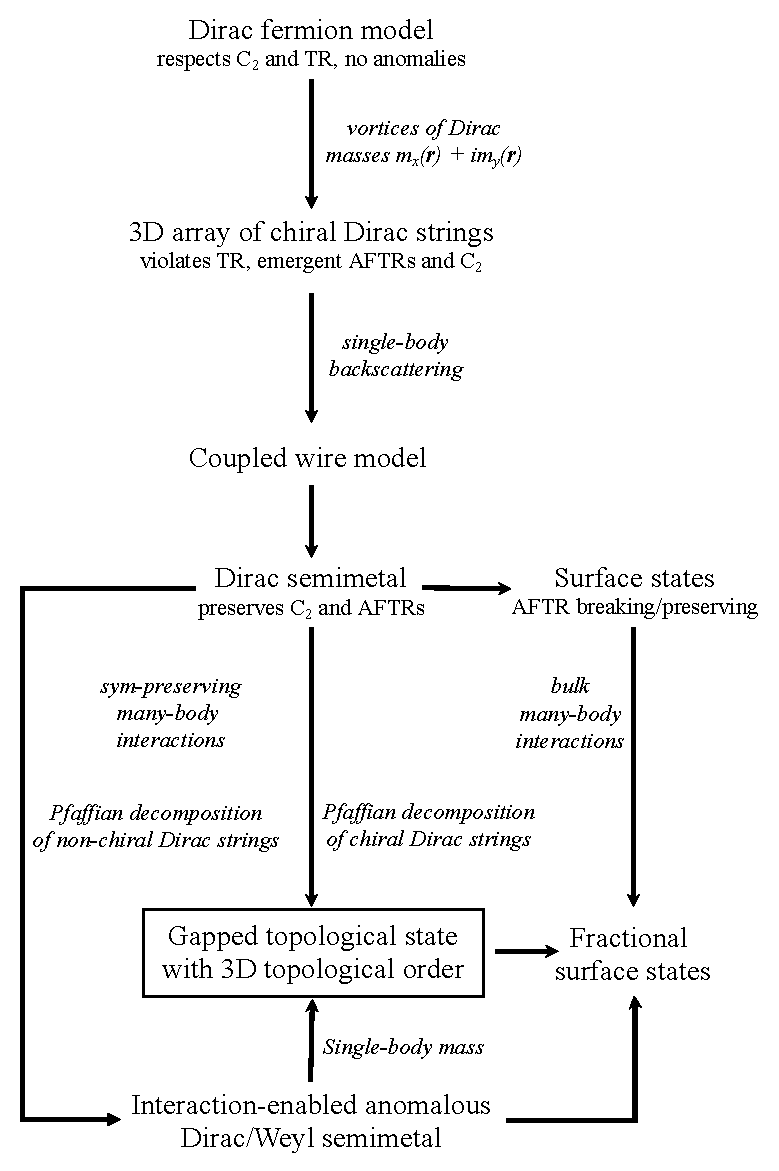
\includegraphics[width=0.8\textwidth]{Flowchart}
	\caption[Logical outline of Model 1 and Model 3.]{Logical outline of Model 1 and Model 3.  It shows the procedure of going from a Dirac fermion model to an interaction-enabled gapped state with three-dimensional topological order. Here, $\mathcal{C}_2$ is the two-fold (screw) rotation symmetry, TR is time-reversal symmetry and AFTR is the antiferromagnetic time-reversal symmetry}\label{fig:Flowchart}
\end{figure}

We then address non-trivial symmetry-preserving many-body interacting effects beyond the single-body mean-field paradigm. We begin with the anisotropic array of chiral Dirac wires that constitutes a Dirac (semi)metal protected by antiferromagnetic time-reversal (\hyperlink{AFTR}{AFTR}) and (screw) $\mathcal{C}_2$ rotation symmetries (Fig.~\ref{fig:WeylTB}). We consider an exactly-solvable model of symmetry-preserving inter-wire many-body backscattering interactions. This model is inspired by and can be regarded as a layered version of the symmetric massive interacting surface state of a topological insulator. It is based on a {\em fractionalization} scheme that divides a single chiral Dirac channel into a decoupled pair of identical chiral ``Pfaffian" channels (Fig.~\ref{fig:glueingsplitting}). Each of these fractional channels carries half of the degrees of freedom of the original Dirac wire. For instance, the fractionalization splits the electric and thermal currents exactly in half. %The bipartition is stabilized by many-body interactions and cannot be realized in any single-body mean-field description. 
It leads to the appearance of fractional quasiparticle excitations. For example, a chiral Pfaffian channel also runs along the 1D edge of the particle-hole symmetric Pfaffian fractional quantum Hall state~\cite{Son15,BarkeshliMulliganFisher15,WangSenthil16}, and supports charge $e/4$ Ising and $e/2$ semionic primary fields.

We consider an explicit combination of many-body interwire backscattering interactions that stabilize the fractionalization. Similar coupled wire constructions were applied in the literature to describe topological insulator's surface state~\cite{MrossEssinAlicea15} and $\nu=1/2$ fractional quantum Hall states~\cite{TeoKaneCouplewires,KaneSternHalperin17}. They are higher dimensional analogues of the Affleck-Kennedy-Lieb-Tasaki (AKLT) spin chain model~\cite{AKLT1,AKLT2}. The pair of chiral Pfaffian channels along each wire is backscattered in opposite directions to neighboring wires by the interaction (Fig.~\ref{fig:gappinginteraction}). As a result of this dimerization of fractional degrees of freedom, the model acquires a finite excitation energy gap and at the same time preserves the relevant symmetries.

We speculate that such a symmetry preserving-gapping by many-body interactions leads to a three-dimensional topological order supporting exotic point-like and line-like quasiparticle excitations with fractional charge and statistics. The complete characterization of the topological order will be part of a future work~\cite{SirotaRazaTeoappearsoon}. Although there have been numerous field-theoretic discussions on possible properties of topologically ordered phases in 3D, this is the first work with a microscopic model that could possibly lead to its material realization.

In the single-body regime, an (antiferromagnetic) time-reversal symmetric Weyl (semi)metal realizable on a three dimensional lattice has a minimum of four momentum-space-separated Weyl nodes. For a single pair of Weyl nodes with opposite chirality, time-reversal symmetry must be broken. However, a key result of this dissertation is the realization of a single pair of momentum-space-separated Weyl nodes in the presence of \AFTR symmetry as enabled by many-body interactions. The coupled wire construction suggests a new {\em interaction-enabled topological (semi)metal} in which these Weyl nodes can be realized (Fig.~\ref{fig:intenable}). 

The many-body interacting coupled-wire model can be turned into a gapless system, where 1) all low-energy degrees of freedom are electronic and freely described in the single-body non-interacting setting by two and only two separated Weyl nodes, 2) the high-energy gapped sector supports fractionalization. Although the model is antiferromagnetic, we conjecture that similar anomalous Weyl (semi)metal can be enabled by interaction while preserving local time-reversal.

The dissertation is organized as follows. In Sec.~\ref{sec:DiracSemimetal}, we construct a single-body coupled wire model of a Dirac/Weyl (semi)metal equipped with two emergent antiferromagnetic time-reversal (\AFTR) axes and a (screw) $\mathcal{C}_2$ rotation symmetry. In Sec.~\ref{sec:anomaly}, we establish the equivalence between the isotropic continuum limit and the anisotropic coupled wire limit by a coarse-graining mapping. We also discuss the anomalous aspects of the pair of Weyl fermions and different resolutions to the anomaly. In Sec.~\ref{sec:fermiarc1}, we describe the gapless surface states of the coupled wire model. \AFTR breaking and preserving surfaces are considered separately in Sec.~\ref{sec:fermiarcAFTRbreaking} and \ref{sec:fermiarcAFTRpreserving} respectively.

In Sec.~\ref{sec:intenable}, we move on to the effect of symmetry-preserving many-body interactions. The fractionalization of a chiral Dirac channel is explained in Sec.~\ref{sec:gluing}, where we establish the Pfaffian decomposition through bosonization techniques. The splitting of a Dirac channel is summarized in Fig.~\ref{fig:fractionalization}. In Sec.~\ref{sec:interactionmodels}, we explicitly construct an exactly-solvable interacting coupled wire model that introduces a finite excitation energy gap to the Dirac system while preserving relevant symmetries. The many-body interwire backscattering interactions are summarized in Fig.~\ref{fig:gappinginteraction}. In Sec.~\ref{sec:AFMstabilization}, we discuss a plausible stabilization mechanism of the desired interactions through an antiferromagnetic order. 

In Sec.~\ref{sec:intenable}, we discuss the other key result of the dissertation, a variation of the model that enables an anomalous topological (semi)metal. We show how a single pair of Weyl nodes in the presence of time-reversal symmetry can be realized through many-body interactions. Such a state is forbidden in the single-body setting. In Sec.~\ref{sec:fracsurface}, we elaborate on the gapless surface states of both new interacting phases discussed in sections~\ref{sec:interactionmodels} and~\ref{sec:intenable}.

We then apply similar techniques to the superconducting analogs of the Dirac semimetals known as the Dirac nodal superconductors in \ref{chap:Model3}. We repeat a similar procedure of building a wire-model and then introduce many-body interactions to gap out the system. 
We construct the many-body gapping potentials that generate a finite energy gap while preserving the underlying symmetries. In the presence of the many-body interactions, we find the emergence of the non-trivial topological orders.
We begin our discussion in Section \ref{sec:coupled} where we detail our construction the coupled wire model of a Dirac nodal superconductor in three spatial dimensions by assembling a vortex array in a microscopic superconductor within the continuum limit. In the continuum model, the massless Dirac fermions are protected by the combination of: local time-reversal symmetry, particle-hole symmetry and glide mirror symmetry. By introducing the array of superconducting pairing vortices, the low-energy electronic degrees of freedom manifest as $(1+1)$-D chiral Dirac fermions that are localized along vortex lines (also referred to as Dirac strings).  Each Dirac string is coupled via single-body tunneling with the adjacent strings, and the couplings reconstruct the Dirac nodal superconductor within the context of the coupled wire model. This anisotropic Dirac nodal superconducting model is protected by the same set of symmetries except time-reversal now becomes non-local and antiferromagnetic. This re-construction enables us to study many-body interactions in three dimensions using bosonization techniques.

With our introduction to the single body physics of the coupled wire methodology complete, in Section \ref{sec:manybody1} we introduce the many-body interactions that preserve all the underlying symmetries. The basic strategy that we follow in this work is based on the bi-partitioning the $SO(2N)$ Kac-Moody current consisting of $N$ chiral Dirac fermions along a vortex. For even $N$, the symmetric gapping interaction can be facilitated by a simple separation $SO(2N)_1\sim SO(N)_1\times SO(N)_1$ of Dirac channels. The model admits a single-body mean-field mass gap, which reflects its trivial topology under the $\mathbb{Z}_2$  classification. On the other hand, due to the presence of the aforementioned symmetries, the odd $N$ case requires a non-trivial string decomposition that involves the level-rank duality $SO(9)_1\sim SO(3)_3\times SO(3)_3$. Consequently, the gapping interactions in the case of odd $N$ lead to fractionalization and non-trivial topological order. In both situations, the gapping potentials are constructed by backscattering the divided Kac-Moody currents to opposite directions between adjacent strings. This results in a finite energy gap while preserving all the underlying symmetries of our model.

Interestingly, when $N=16$, we find a special form of the decomposition, $SO(32)\sim E_8 \times E_8$, that utilizes the $E_8$ unimodular lattice. We find that this decomposition results in the many-body interaction that has trivial topological order. 
%%
%

%
\chapter{Model 1: Dirac and Weyl Semimetals}\label{chap:Model1}

\section{Introduction}\label{sec:introduction}
Dirac and Weyl semimetals are nodal electronic phases of matter in three spatial dimensions. Their low-energy emergent quasiparticle excitations are electronic Dirac~\cite{Dirac28} and Weyl~\cite{Weyl29} fermions. (Contemporary reviews in condensed electronic matter can be found in Ref.~\cite{Ashvin_Weyl_review,TurnerVishwanath13,HasanXuBian15,RMP,Burkov16,JiaXuHasan16,ArmitageMeleVishwanath16,YanFelser17}.) They are three dimensional generalizations of the Dirac fermions that appear in two dimensional graphene~\cite{NetoGuineaPeresNovoselovGeim09} and the surface boundary of a topological insulator~\cite{HasanKane10,QiZhangreview11,HasanMoore11,RMP}. They follow massless quasi-relativistic linear dispersions near nodal points in the energy-momentum space close to the Fermi level. Contrary to accidental degeneracies which can be lifted by generic perturbations, these nodal points are protected by topologies or symmetries. 

A Weyl fermion is {\em chiral} and has a non-trivial winding of a pseudo-spin texture near the singular nodal point in energy-momentum space. This would associate to a non-conservative charge current under a parallel electric and magnetic field and is known as the Adler-Bell-Jackiw (\hypertarget{ABJ}{ABJ}) anomaly~\cite{Adler69,BellJackiw69}. Thus, in a true three dimensional lattice system, Weyl fermions must come in pairs~\cite{Nielsen_Ninomiya_1981,NielsenNinomiyaPLB1981,NielsenNinomiya83} so that the net chirality, and consequently the anomaly, cancels. Or otherwise, a three dimensional system of a single Weyl fermion must be holographically supported as the boundary of a topological insulator in four dimensions~\cite{ZhangHu01,BernevigChernHuToumbasZhang02,QiHughesZhang08}. On the other hand, a Dirac fermion in three dimensions consists of a pair of Weyl fermions with opposite chiralities. Without symmetries, it is not stable and can turn massive upon inter-Weyl-species coupling. With symmetries, a band crossing can be protected by the distinct symmetry quantum numbers the bands carry along a high symmetry axis. In this article, we focus on the fourfold degenerate Dirac nodal point protected by time-reversal (\hypertarget{TR}{TR}) and (screw) rotation symmetry.

In electronic systems, massless Dirac and Weyl fermions appear in gap-closing phase transitions between spin-orbit coupled topological insulators and normal insulators~\cite{Murakami2007}. When inversion or time-reversal symmetry is broken, nodal Weyl points can be separated in energy-momentum space. Such gapless electronic phases are contemporarily referred to as Weyl (semi)metals~\cite{WanVishwanathSavrasovPRB11,YangLuRan11,burkovBalenstPRL11,BurkovBalentsPRB11}. Their boundary surfaces support open Fermi arcs~\cite{WanVishwanathSavrasovPRB11} that connect surface-projected Weyl nodes. Weyl (semi)metals also exhibit exotic transport properties, such as negative magneto-resistance, non-local transport, chiral magnetic effect, and chiral vortical effect~\cite{Burkov_Weyl_electromagnetic_2012,Hosur_Weyl_develop,Lu_anomaly_Weyl_2013,SonSpivak13,Sid_anomaly_Weyl,Marcel_Weyl_response}. There have been numerous first principle calculations~\cite{WengXiZhong16} on proposed materials such as the non-centrosymmetric (La/Lu)Bi$_{1-x}$Sb$_x$Te$_3$~\cite{LiuVanderbilt14}, the TlBiSe$_2$ family~\cite{SinghSharmaLinHasanPrasadBansil12}, the TaAs family~\cite{WengBernevigDai2015,HuangXuZahidTaAs2015}, trigonal Se/Te~\cite{HirayamaOkugawaIshibashiMurakamiMiyake15} and the HgTe class~\cite{RuanXing16}, as well as the time-reversal breaking pyrochlore iridates \cite{WanVishwanathSavrasovPRB11,witczak_kim_weyl_2012,chen_hermele_weyl}, magnetically doped topological and trivial insulator multilayers \cite{burkovBalenstPRL11}, HgCr$_2$Se$_4$~\cite{XuWengWangDaiFang11} and Hg$_{1-x-y}$Cd$_x$Mn$_y$Te~\cite{BulmashLiuQi14}. At the same time, there have also been abundant experimental observations in bulk and surface energy spectra~\cite{HasanXuBelopolskiHuang17} as well as transport~\cite{WangLinWangYuLiao17}. Angle-resolved photoemission spectroscopy (\hypertarget{ARPES}{ARPES}) showed bulk Weyl spectra and surface Fermi arcs in TaAs~\cite{Xu_Weyl_2015_first,Weyl_discovery_TaAs,YangLiuChenTaAs2015,TaAs_Weyl_obeservationDing,BelopolskiZahid16} as well as similar materials such as NbAs, NbP and TaP~\cite{XuNbAs15,LiuChen16}. Other materials such as Ag$_3$BO$_3$, TlTe$_2$O$_6$ and Ag$_2$Se~\cite{ChangHasan16} were observed to host pinned Weyl nodes at high symmetry points. %theory pinned along screw axis {TsirkinSouzaVanderbilt17}
Negative magneto-resistance was reported in TaAs~\cite{Huang_Weyl_2015,Zhang_anomaly_Weyl_2015} as a suggestive signature of the \ABJ anomaly. Similar properties were also observed in TaP~\cite{HuMaoTaP17}, NbP and NbAs~\cite{CorinnaNiemannFelserNbP17,LiXuNbAsNbP17,GoothNielschNbP17}, although not without controversies~\cite{SudeshPatnaikNbP17}. 

Weyl points with opposite chiralities cannot be separated in energy-momentum space when both inversion and time reversal symmetries are present. Massless Dirac fermions appear between gap-closing phase transitions between topological and trivial (crystalline) insulators, such as Bi$_{1-x}$Sb$_x$~\cite{TeoFuKane08} and Pb$_{1-x}$Sn$_x$Te~\cite{Hsieh:2012fk}. Critical Dirac (semi)metals were investigated for example in the tunable TlBiSe$_{2-x}$S$_x$~\cite{SatoTakahashi11,SoumaAndo12,XuCavaHasan11}, Bi$_{2−x}$In$_x$Se$_3$~\cite{BrahlekSeongshik12,WuArmitage13} and Hg$_{1-x}$Cd$_x$Te~\cite{OrlitaPotemski14}, as well as the charge balanced BaAgBi~\cite{DuWanXYBi15}, PtBi$_2$, SrSn$_2$As$_2$~\cite{GibsonCava15} and ZrTe$_5$~\cite{LiVallaZrTe516} whose natural states are believed to be close to a topological critical transition. A Dirac (semi)metallic phase can be stabilized when the Dirac band crossing is secured along a high symmetry axis and the two crossing bands carry distinct irreducible representations. Theoretical studies include the diamond-structured $\beta$-crystobalite BiO$_2$ family~\cite{BiO3_Dirac_semimetal} (space group (\hypertarget{SG}{SG}) No.~227, Fd3m), the orthorhombic body-centered BiZnSiO$_4$ family~\cite{SteinbergYoungZaheerKaneMeleRappe14} (\SG No.~74, Imma), the tetragonal Cd$_3$As$_2$~\cite{wangCd3As2PRB13} (\SG No.~142, I4$_1$/acd), the hexagonal Na$_3$Bi family~\cite{Dai_predition_Na3Bi}, as well as the filling-enforced non-symmorphic Dirac semimetals~\cite{KonigMermin97,ParameswaranTurnerArovasVishwanath13,WatanabePoVishwanathZaletel15,ChenKimKee16,WatanabePoZaletelVishwanath16,BradlynBernevig17} such as the hexagonal TlMo$_3$Te$_3$ family~\cite{GibsonCava15} (\SG No.~176, P6$_3$/m), the monoclinic Ca$_2$Pt$_2$Ga (\SG No.~15, C2/c), AgF$_2$, Ca$_2$InOsO$_6$ (\SG No.~14, P2$_1$/n), and the orthorhombic CsHg$_2$ (\SG No.~74, Imma)~\cite{ChenPoNeatonVishwanath16}. At the same time, there are numerous experimental confirmations. They include \ARPES observations on Cd$_2$As$_3$~\cite{Cd3As2Chen2014,neupaneDiracHasan,borisenkoPRLCd3As2}, Na$_3$Bi~\cite{Liu21022014,Xu18122014} and ZrTe$_5$~\cite{LiVallaZrTe516}; scanning tunneling microscopy in Cd$_2$As$_3$~\cite{Yazdani_CdAs}; magneto-transport in Bi$_{1-x}$Sb$_x$~\cite{KimLiBiSb13}, Cd$_2$As$_3$~\cite{liangOngTransportCd3As2,HeLi14,XiangChen15,FengLuCd3As215,LiYuCd3As215,LiWangCd3As216,GuoLeeCd2As316,ZhangXiuCd3As217}, Na$_3$Bi~\cite{Xu18122014,XiongOng15}, ZrTe$_5$~\cite{ZhengMingliangZrTe514,LiVallaZrTe516,LiangOngHallZrTe516,YuanXiuZrTe516}, HfTe$_5$~\cite{WangWangHfTe516} and PtBi$_2$~\cite{GaoTianPtBi217}; magneto-optics~\cite{AkrapOrlitaCd2As316} and anomalous Nernst effect~\cite{LiangOngNernstCd3As217} in Cd$_2$As$_3$, and many more. However, there are also contradicting pieces of evidence, especially in ZrTe$_5$ and HfTe$_5$ that suggest a bulk band gap~\cite{WengDaiFangZrTe514,LiXingZrTe516,WuPanZrTe516,MoreschiniGrioniZrTe516,ManzoniCrepaldiZrTe516,ManzoniParmigianiZrTe517,FanZhouZrTe517}.
%Cd3As2
%SdH\cite{HeLi14,XiangChen15,GuoLeeCd2As316} negative magnetoresistance\cite{liangOngTransportCd3As2} anomalous Nernst effect\cite{LiangOngNernstCd3As217} magneto-optics\cite{AkrapOrlitaCd2As316}
%Na3Bi
%negative magnetoresistance\cite{Xu18122014,XiongOng15}
%ZrTe5
%negative magnetoresistance\cite{ZhengMingliangZrTe514,LiVallaZrTe516} anomalous Hall\cite{LiangOngHallZrTe516}
%HfTe5
%negative magnetoresistance\cite{WangWangHfTe516}
%PtBi2
%magnetoresistance\cite{GaoTianPtBi217}

\begin{figure}[htbp]
	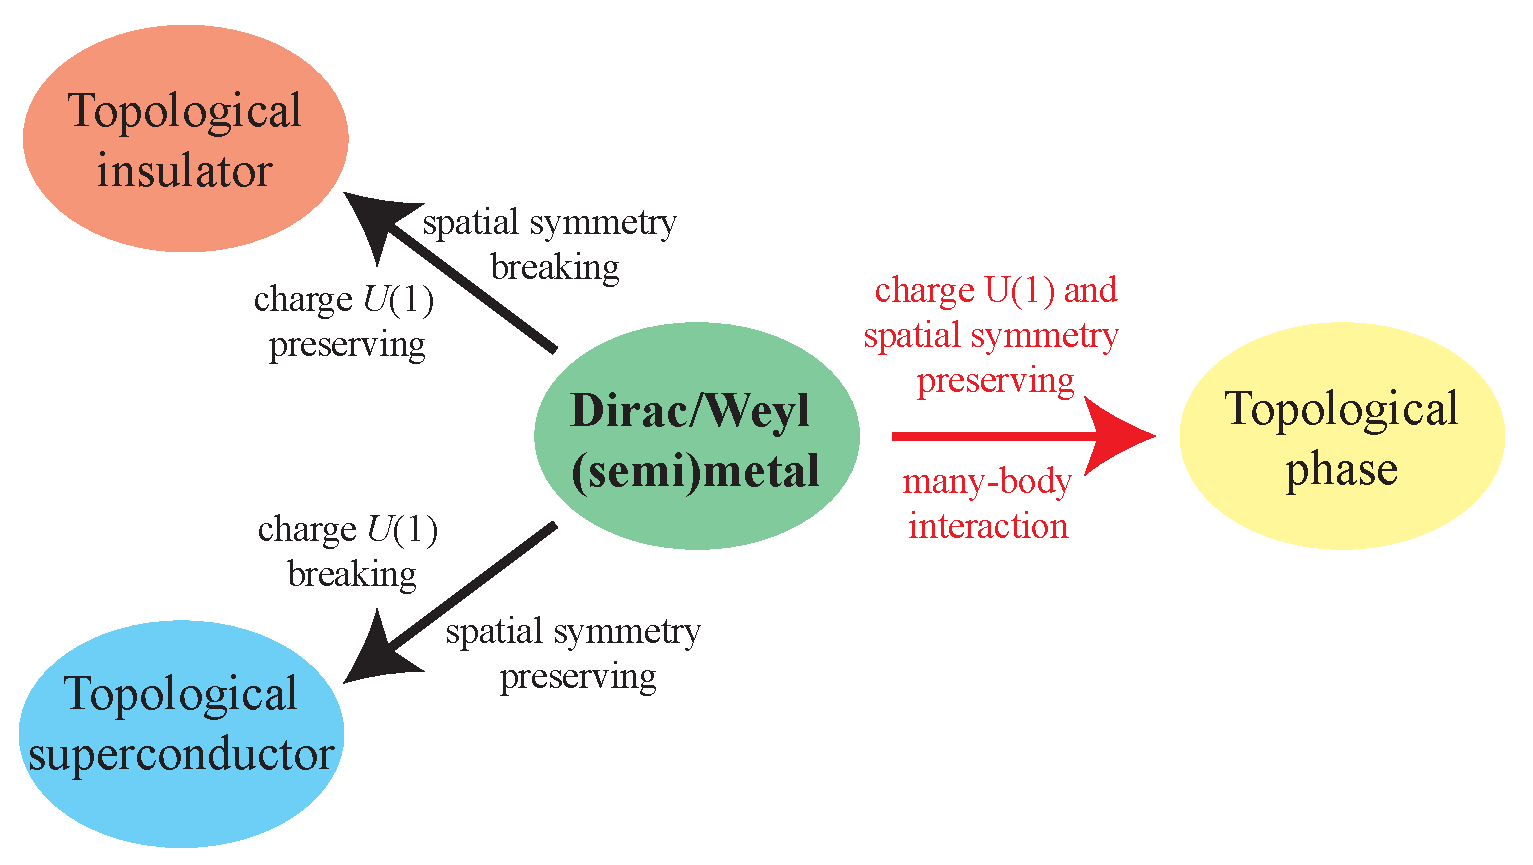
\includegraphics[width=0.9\textwidth]{intro}
	\caption{Symmetry breaking single-body gapping versus symmetry preserving many-body gapping of a Dirac/Weyl (semi)metal.}\label{fig:intro}
\end{figure}

Dirac/Weyl (semi)metals are the origins of a wide variety of topological phases in three dimensions (see Fig.~\ref{fig:intro}). By introducing a spatial or charge $U(1)$ symmetry-breaking single-body mass, they can be turned into a topological insulator or superconductor. The focus of this manuscript is on symmetry-preserving many-body gapping interactions. The resulting insulating topological phase can carry long-range entanglement and a non-trivial topological order. Similar phenomena were theoretically studied on the Dirac surface state of a topological insulator~\cite{WangPotterSenthilgapTI13,MetlitskiKaneFisher13b,ChenFidkowskiVishwanath14,BondersonNayakQi13} and the Majorana surface state of a topological superconductor~\cite{LukaszChenVishwanath,MetlitskiFidkowskiChenVishwanath14}, where symmetry-preserving many-body gapping interactions are possible and lead to non-trivial surface topological orders that support anyonic quasiparticle excitations.

Symmetry-preserving gapping interactions cannot be studied using a single-body mean-field theory. This is because the Dirac/Weyl (semi)metallic phase is protected by symmetries in the single-body setting and any mean-field model with an excitation energy gap must therefore break the symmetry either explicitly or spontaneously. The coupled wire construction can serve as a powerful tool in building an exactly-solvable interacting model and understanding many-body topological phases of this sort. The construction involves a highly anisotropic approximation where the electronic degrees of freedom are confined along an array of continuous one-dimensional wires. Inspired by sliding Luttinger liquids~\cite{OHernLubenskyToner99,EmeryFradkinKivelsonLubensky00,VishwanathCarpentier01,SondhiYang01,MukhopadhyayKaneLubensky01}, the coupled wire construction was pioneered by Kane, Mukhopadhyay and Lubensky~\cite{KaneMukhopadhyayLubensky02} in the study of Laughlin~\cite{Laughlin83} and Haldane-Halperin hierarchy~\cite{Haldane83,Halperin84} fractional quantum Hall states. Later, this theoretical technique was applied in more general fractional quantum Hall states~\cite{TeoKaneCouplewires,KlinovajaLoss14,MengStanoKlinovajaLoss14,SagiOregSternHalperin15,KaneSternHalperin17}, anyon models~\cite{OregSelaStern14,StoudenmireClarkeMongAlicea15}, spin liquids~\cite{MengNeupertGreiterThomale15,GorohovskyPereiraSela15}, (fractional) topological insulators~\cite{NeupertChamonMudryThomale14,KlinovajaTserkovnyak14,SagiOreg14,SagiOreg15,SantosHuangGefenGutman15} and superconductors~\cite{mongg2,SeroussiBergOreg14}, as well as the exploration of symmetries and dualities~\cite{MrossAliceaMotrunich16,MrossAliceaMotrunich17}. Moreover, coupled wire construction has already been used to investigate three dimensional fractional topological phases~\cite{Meng15,IadecolaNeupertChamonMudry16,IadecolaNeupertChamonMudry17} and Weyl (semi)metal~\cite{Vazifeh13} even in the strongly-correlated fractional setting~\cite{MengGrushinShtengelBardarson16}. 

The microscopic symmetry-preserving many-body interactions in the Dirac surface state on a topological insulator was discussed by Mross, Essin and Alicea in Ref.\cite{MrossEssinAlicea15}. They mimicked the surface Dirac modes using a coupled wire model and proposed explicit symmetric many-body interactions that lead to a variation of gapped and gapless surface states. Motivated by this and also using a coupled wire construction, the microscopic symmetry-preserving many-body gapping of the Majorana topological superconducting surface state was studied by one of us in Ref.\cite{SahooZhangTeo15}. 

In this article, we focus on (i) a coupled wire realization of a Dirac/Weyl (semi)metallic phase protected by antiferromagnetic time-reversal (\hypertarget{AFTR}{AFTR}) and screw twofold rotation symmetries, (ii) a set of exactly-solvable inter-wire many-body interactions that introduces a finite excitation energy gap while preserving the symmetries, and (iii) an interaction-enabled (semi)metallic electronic phase which is otherwise forbidden by symmetries in the single-body setting.

\section{Coupled Wire model of Dirac Semimetals}\label{sec:DiracSemimetal}
We begin with a Dirac semimetal in three dimensions. It consists of a pair of massless Weyl fermions with opposite chiralities. In this article we do not distinguish between a Dirac and a Weyl semimetal. This is because the fermion doubling theorem~\cite{Nielsen_Ninomiya_1981,NielsenNinomiyaPLB1981,NielsenNinomiya83} and the absence of the Adler-Bell-Jackiw anomaly~\cite{Adler69,BellJackiw69} require Weyl fermions to always come in pairs in a three dimensional lattice system. A Weyl semimetal therefore carries the same low energy degrees of freedom as a Dirac semimetal. We refer to the case when the pair of Weyl fermions are separated in momentum space as a translation symmetry protected Dirac semimetal. Here, we assume the simplest case where the two Weyl fermions overlap in energy-momentum space. Its low-energy band Hamiltonian takes the spin-orbit coupled form \begin{align}H^0_{\mathrm{Dirac}}({\bf k})=\hbar v{\bf k}\cdot\vec{s}\mu_z \,, \label{DiracHam0}\end{align} where $\vec{s}=(s_x,s_y,s_z)$ are the spin-$1/2$ Pauli matrices, and $\mu_z=\pm1$ indexes the two Weyl fermions.

\begin{figure}[htbp]
	\centering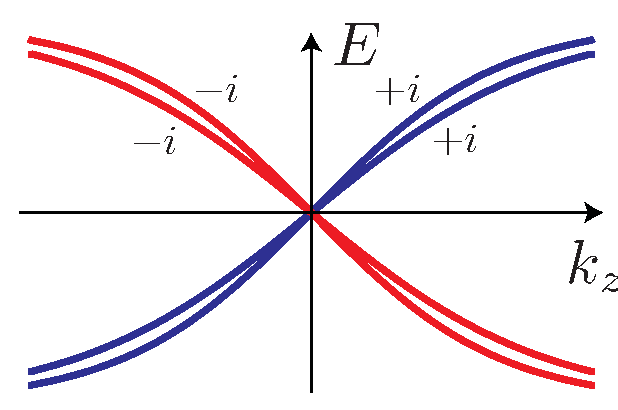
\includegraphics[width=0.5\textwidth]{Diracbands}
	\caption[The two pairs of counter-propagating Dirac bands.]{The two pairs of counter-propagating Dirac bands along the $k_z$-axis distinguished by eigenvalues of $C_2=\pm i$.}\label{fig:Diracbands}
\end{figure}

Normally the masslessness of the Dirac system is protected by a set of symmetries. Here, we assume the time reversal (TR) $\mathcal{T}$, which is represented in the single-body picture by the spinful operator $\hat{T}=is_y\mathcal{K}$ where $\mathcal{K}$ is the complex conjugation operator, and a twofold rotation $C_2$ about the $z$-axis. In the case when $\mu_z$ has a non-local origin such as sublattice or orbital, it can enter the rotation operator. We assume $\mathcal{C}_2$ is represented in the single-body picture by $\hat{C}_2=is_z\mu_z$. It squares to minus one in agreement with the fermionic statistics, and commutes with the local \TR operator. In momentum space, $\mathcal{T}$ flips ${\bf k}\to-{\bf k}$ while $C_2$ rotates $(k_x,k_y,k_z)\to(-k_x,-k_y,k_z)$. The band Hamiltonian \eqref{DiracHam0} shares simultaneous eigenstates with $C_2$ along the $k_z$-axis. The two forward moving bands have $C_2$ eigenvalues $+i$ while the two backward moving ones have $C_2$ eigenvalues $-i$ (see Fig.~\ref{fig:Diracbands}). Therefore the band crossing is $C_2$-protected while the fourfold degeneracy is pinned at ${\bf k}=0$ because of \TR symmetry. Noticing that each of the $C_2=\pm i$ sector along the $k_z$-axis is chiral (i.e.~consisting of a single propagating direction), it violates the fermion doubling theorem~\cite{Nielsen_Ninomiya_1981,NielsenNinomiyaPLB1981} and is anomalous. This can be resolved by assuming the $C_2$ symmetry is actually a non-symmorphic screw rotation in the microscopic lattice limit and squares to a primitive lattice translation in $z$. $k_z$ is now periodically defined (up to $2\pi/a$) and the two $C_2$ eigen-sectors wraps onto each other after each period. Focusing on the continuum limit where $k_z$ is small (when compared with $2\pi/a$), $C_2^2=-e^{ik_za}\approx-1$ and the $C_2$ symmetry behaves asymptotically as a proper rotation.

The primary focus of this article is to explore symmetry preserving/enabled interacting topological states that originate from the massless Dirac system. Contrary to its robustness in the single-body non-interacting picture, we show that the 3D Dirac fermion can acquire a many-body mass gap without violating the set of symmetries. To illustrate this, we first make use of the fact that the Dirac system can be turned massive by breaking symmetries. Symmetry breaking inter-valley scatterings introduce two coexisting mass terms \begin{align}H_{\mathrm{Dirac}}({\bf k},{\bf r})=H_{\mathrm{Dirac}}^0({\bf k})+m_x({\bf r})\mu_x+m_y({\bf r})\mu_y \,, \label{DiracHam}\end{align} where $m_x$ (or $m_y$) preserves (resp.~breaks) \TR, and both of them violate $C_2$. We allow slow spatial modulation of the mass parameters, which can be grouped into a single complex parameter $m({\bf r})=m_x({\bf r})+im_y({\bf r})$, and to be precise, momentum ${\bf k}$ should be taken as a differential operator $-i\nabla_{\bf r}$ when translation symmetry is broken. Non-trivial spatial windings of the symmetry breaking mass parameters give rise to topological line defects or vortices that host protected low-energy electronic degrees of freedom. Proliferation of interacting vortices then provides a theoretical path to multiple massive/massless topological phases while restoring and modifying the original symmetries as they emerge in the low-energy long-length scale effective theory.

\begin{figure}[htbp]
	\centering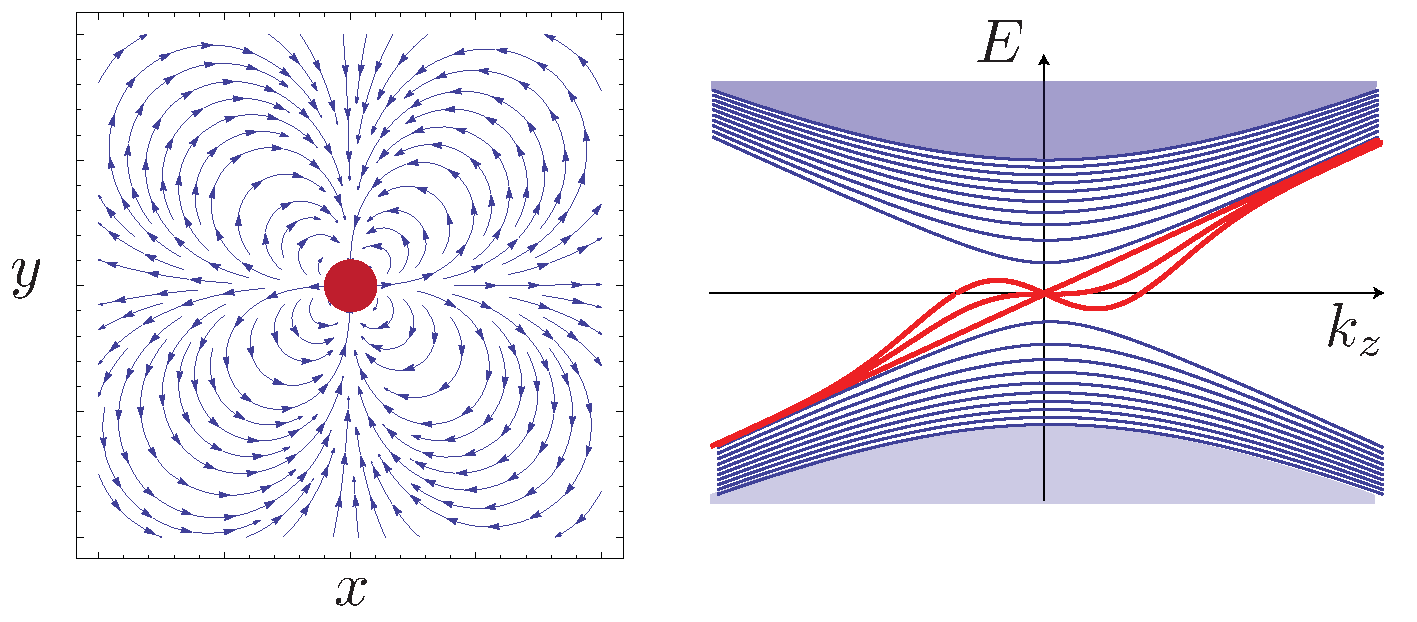
\includegraphics[width=0.8\textwidth]{Diracstring}
	\caption[Spatial winding of mass parameters around a Dirac string.]{Dirac string. (Left) Spatial winding of mass parameters around a Dirac string going out of the paper represented by the center red dot. Stream lines represent the vector field ${\bf m}({\bf r})=(m_x({\bf r}),m_y({\bf r}))$. (Right) Energy spectrum of chiral Dirac fermions. Blue bands represent bulk continuum. Red bands correspond to chiral Dirac fermions localized along the string.}\label{fig:Diracstring}
\end{figure}

A topological line defect is a vortex string of the mass parameter in three dimensions where the complex phase of $m({\bf r})=|m({\bf r})|e^{i\varphi({\bf r})}$ winds non-trivially around the string. The left diagram in Fig.~\ref{fig:Diracstring} shows the spatial modulation of $\varphi({\bf r})$ along the $xy$ cross-sectional plane normal to a topological line defect, which runs along the $z$ axis. In this example, the complex phase $\varphi({\bf r})$ winds by $6\pi$ around the line defect (represented by the red dot at the origin). The winding number of the complex phase in general can be evaluated by the line integral \begin{align}c=\frac{1}{2\pi}\oint_\mathcal{C}d\varphi({\bf r})=\frac{1}{2\pi i}\oint_\mathcal{C}\frac{\nabla_{\bf r}m({\bf r})}{m({\bf r})}\cdot d{\bf r} \,, \label{winding}\end{align} where $\mathcal{C}$ is a (righthanded) closed path that runs once around the (oriented) line defect. Eq.\eqref{winding} is always an integer given that the mass parameter $m({\bf r})$ is non-vanishing along $\mathcal{C}$.

Massless chiral Dirac fermions run along these topological line defects~\cite{TeoKane}. When focusing at $k_z=0$, the differential operator \eqref{DiracHam} with a vortex along the $z$-axis is identical to the 2D Jackiw-Rossi model~\cite{JackiwRossi81} with chiral symmetry $\gamma_5=s_z\mu_z$. Each zero energy mode corresponds to a massless chiral Dirac fermion with positive or negative group velocity in $z$ depending on the sign of its $\gamma_5$ eigenvalue. (For a concrete example, see appendix~\ref{sec:chiralmodesapp}) These quasi-one dimensional low-energy electronic modes are similar to those that run along the edge of 2D Landau levels and Chern insulators, except they are now embedded in three dimensions. Their wave functions extend along the defect string direction but are localized and exponentially decay away from the defect line. Moreover, such an electronic channel is chiral in the sense that there is only a single propagating direction. The energy spectrum of the topological line defect (for the example with winding number $c=3$) is shown in the right diagram of Fig.~\ref{fig:Diracstring}, in which, there are three chiral bands (red curves) inside the bulk energy gap representing the 3 chiral Dirac electrons. As a consequence of the chirality, the transport of charge and energy must also be uni-directional. The chiral electric and energy-thermal responses are respectively captured by the two conductances \begin{align}\sigma=\frac{\delta I_{\mathrm{electric}}}{\delta V}=\nu\frac{e^2}{h},\quad\kappa=\frac{\delta I_{\mathrm{energy}}}{\delta T}=c\frac{\pi^2k_B^2}{3h}T \,, \label{conductance}\end{align} where $\nu$ is the filling fraction if the chiral channel is supported by a 2D insulating bulk, and $c$ is called the chiral central charge. For the Dirac case, $c=\nu$ is the number of chiral Dirac channels. Here $c$ can be negative when the Dirac fermions oppose the preferred orientation of the topological line defect. In a more general situation, $c=c_R-c_L$ counts the difference between the number of forward propagating and backward propagating Dirac fermions. There is a mathematical index theorem~\cite{TeoKane,AtiyahSinger63,Nakaharabook} that identifies the topological winding number in \eqref{winding} and the analytic number of chiral Dirac fermions in \eqref{conductance}. Hence, there is no need to distinguish the two $c$'s. 

The massless chiral Dirac channels, described by the low-energy effective theory \begin{align}\mathcal{L}_{\mathrm{Dirac}}=i\sum_{a=1}^{c_R}\psi^\dagger_a(\partial_t+\tilde{v}\partial_x)\psi_a+i\sum_{b=c_R+1}^{c_R+c_L}\psi^\dagger_b(\partial_t-\tilde{v}\partial_x)\psi_b\label{lowenergy}\end{align} have an emergent conformal symmetry and the index $c=c_R-c_L$ is also the chiral central charge of the effective conformal field theory (\hypertarget{CFT}{CFT}). We refer to the primitive topological line defect with $c=\pm1$ that hosts one and only chiral Dirac fermion $\psi$ as a {\em Dirac string}. (It should not be confused with the Dirac magnetic flux string that connects monopoles.)

\begin{figure}[htbp]
	\centering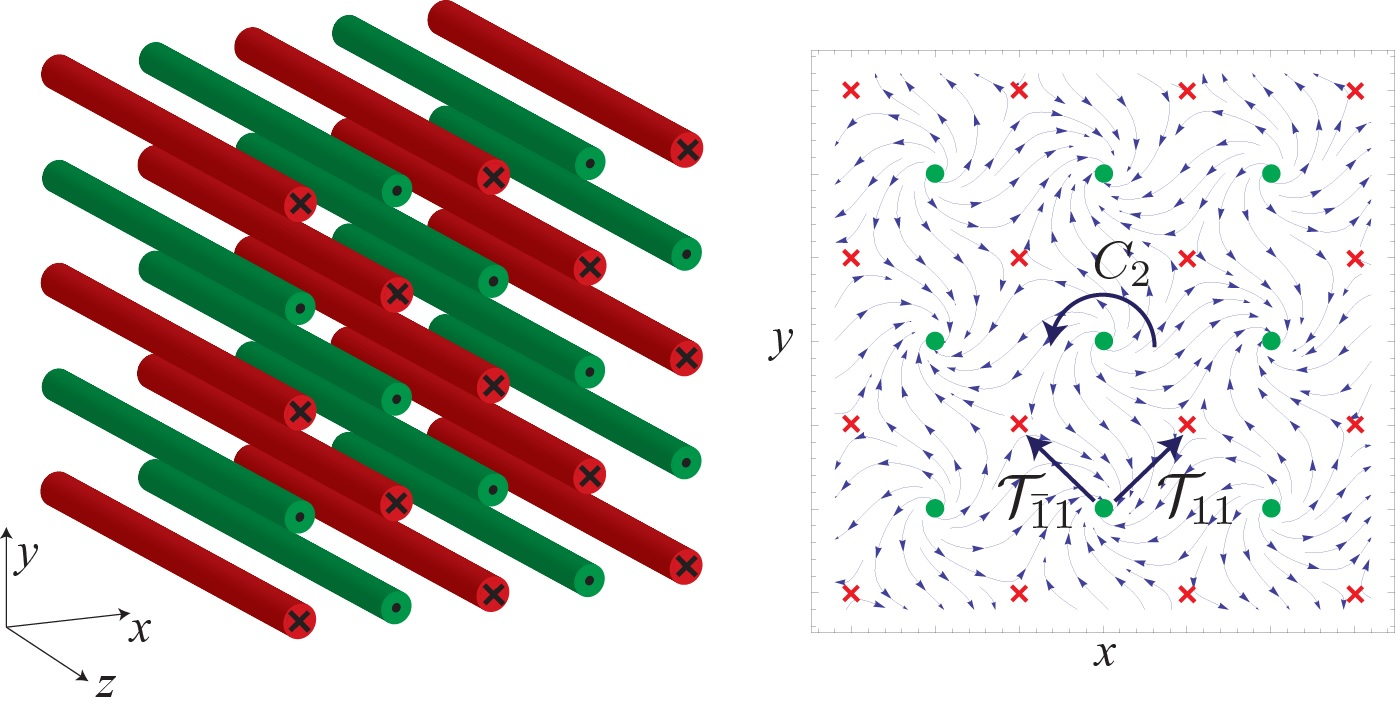
\includegraphics[width=0.9\textwidth]{vortexlattice.jpg}
	\caption[(Left) A 3D array of Dirac strings. (Right) Cross section of the array.]{(Left) A 3D array of Dirac strings. (Right) Cross section of the array. {\color{red}$\boldsymbol\times$} associates into-the-plane Dirac channel, {\color{green}$\bullet$} represents out-of-plane ones. Stream lines represent the configuration of the mass parameter vector field ${\bf m}({\bf r})=(m_x({\bf r}),m_y({\bf r}))$ of the vortex lattice.}\label{fig:vortexlattice}
	\centering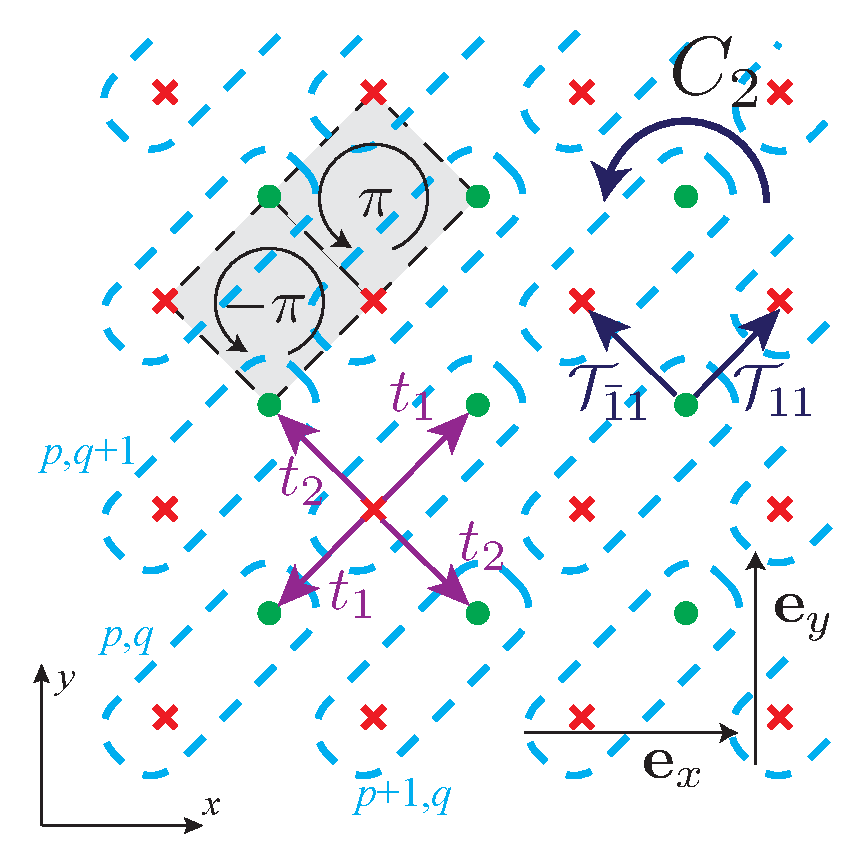
\includegraphics[width=0.5\textwidth]{WeylTB}
	\caption[Coupled Dirac wire model with tunneling amplitudes.]{Coupled Dirac wire model with tunneling amplitudes $t_1,t_2$. Each unit cell (dashed box) consists a pair of counter-propagating Dirac strings, {\color{red}$\boldsymbol\times$} and {\color{green}$\bullet$}. $\mathcal{T}_{11},\mathcal{T}_{\bar{1}1}$ are the two anti-ferromagnetic directions.}\label{fig:WeylTB}
\end{figure}

A three-dimensional array of Dirac strings (wires) can be realized as a vortex lattice of the mass parameter $m=m_x+im_y$ in a Dirac semimetal. For example, Fig.~\ref{fig:vortexlattice} shows a vortex lattice generated by the spatially-varying Dirac mass \begin{align}m({\bf r})=m_0\frac{\mathrm{sd}(x+iy)}{|\mathrm{sd}(x+iy)|},\label{Jacobielliptic}\end{align} where $\mathrm{sd}$ is the (rescaled) Jacobian elliptic function~\cite{ReinhardtWalker10} with simple zeros at $p+iq$ and poles at $(p+1/2)+i(q+1/2)$ for $p,q$ integers. It consists of vortices with alternating winding number $c=\pm1$ at the zeros and poles in a checkered board lattice configuration. On the cross section plot on the right side of Fig.~\ref{fig:vortexlattice}, there is a Dirac string with positive (or negative) winding at each {\color{green}$\bullet$} (resp. {\color{red}$\boldsymbol\times$}). Each vortex string has a chiral Dirac fermion running through it. Figure~\ref{fig:WeylTB} shows the same two-dimensional slice of the array, except suppressing the mass parameters which correspond to irrelevant microscopic high-energy degrees of freedom. We choose a unit cell labeled by $(p,q)$, its $x,y$ coordinates. Each has both a forward moving Dirac fermion $\psi_{p,q}^\odot$ (shown as {\color{green}$\bullet$}) and a backward moving one $\psi_{p,q}^\otimes$ (shown as {\color{red}$\boldsymbol\times$}). 

This array configuration breaks \TR as the symmetry would have reversed the chirality (i.e.~propagating direction) of each Dirac fermion. Instead, it has an emergent {\em anti-ferromagnetic time reversal} (AFTR) symmetry, which is generated by the operators $\mathcal{T}_{11}$ and $\mathcal{T}_{\bar{1}1}$ in the diagonal and off-diagonal directions. Each is composed of a time reversal operation and a half-translation by $({\bf e}_x+{\bf e}_y)/2$ or $(-{\bf e}_x+{\bf e}_y)/2$. \begin{gather}\mathcal{T}_{11}\psi_{p,q}^\otimes\mathcal{T}_{11}^{-1}=\psi_{p,q}^\odot,\quad\mathcal{T}_{11}\psi_{p,q}^\odot\mathcal{T}_{11}^{-1}=-\psi_{p+1,q+1}^\otimes\nonumber\\\mathcal{T}_{\bar{1}1}\psi_{p,q}^\otimes\mathcal{T}_{\bar{1}1}^{-1}=\psi_{p-1,q}^\odot,\quad\mathcal{T}_{\bar{1}1}\psi_{p,q}^\odot\mathcal{T}_{\bar{1}1}^{-1}=-\psi_{p,q+1}^\otimes \,. \label{AFTR}\end{gather} These \AFTR operators are non-local as they come with lattice translation parts. They are anti-unitary in the sense that $\mathcal{T}\alpha\psi\mathcal{T}^{-1}=\alpha^\ast\mathcal{T}\psi\mathcal{T}^{-1}$ and $\langle\mathcal{T}u|\mathcal{T}v\rangle=\langle u|v\rangle^\ast$ because the local time reversal symmetry is anti-unitary. %Normally the local \TR operation for a spinful fermion squares to minus one. However, the non-local nature of the \AFTR symmetry allows us to absorb the sign by a non-local gauge transformation (for example $\psi^{\otimes/\odot}_{p,q}\to(-1)^q\psi^{\otimes/\odot}_{p,q}$) so that no signs appear in \eqref{AFTR}. 
Similar to a spatial non-symmorphic symmetry, the \AFTR symmetries square to the primitive translation operators \begin{align}\mathcal{T}_{11}\mathcal{T}_{\bar{1}1}&=(-1)^F\mbox{translation}({\bf e}_y),\nonumber\\\mathcal{T}_{11}\mathcal{T}_{\bar{1}1}^{-1}&=\mbox{translation}({\bf e}_x),\label{AFTRalg}\end{align} where $(-1)^F$ is the fermion parity operator. Moreover they mutually commute $[\mathcal{T}_{11},\mathcal{T}_{\bar{1}1}]=0$. We notice in passing that the \AFTR symmetry is only an emergent symmetry in the low-energy effective theory. It is not preserved in the microscopic Dirac model \eqref{DiracHam} and is broken by the mass parameter, $m({\bf r})\neq m({\bf r}+({\bf e}_x\pm{\bf e}_y)/2)^\ast$. For instance, the Jacobian elliptic Dirac mass function \eqref{Jacobielliptic} actually has a periodic unit cell twice the size of that of the effective wire model in Fig.~\ref{fig:WeylTB}. On the other hand, the Dirac mass \eqref{Jacobielliptic} is odd under $C_2$, $m(C_2{\bf r})=-m({\bf r})$. This sign is canceled by the $C_2$ rotations of the Dirac matrices, $\hat{C}_2\mu_{x,y}\hat{C}_2^{-1}=-\mu_{x,y}$, that couple with the Dirac mass in the Hamiltonian \eqref{DiracHam}. Therefore the Dirac wire model in Fig.~\ref{fig:WeylTB} has a twofold axis along one of the Dirac string, say $\psi^\odot_{0,0}$. The Dirac channel fermions transform unitarily according to \begin{align}\mathcal{C}_2\psi^\odot_{p,q}\mathcal{C}_2^{-1}=i\psi^\odot_{-p,-q},\quad\mathcal{C}_2\psi^\otimes_{p,q}\mathcal{C}_2^{-1}=-i\psi^\otimes_{-p+1,-q+1},\label{C2}\end{align} where the factor of $i$ ensures the fermionic $-1$ twist phase for a $2\pi$ rotation, and the second eqaulity in \eqref{C2} is determined by the first one together with \eqref{AFTR} and the symmetry relations \begin{gather}\mathcal{C}_2\mathcal{T}_{11}=(-1)^F\mathcal{T}_{11}^{-1}\mathcal{C}_2,\quad\mathcal{C}_2\mathcal{T}_{\bar{1}1}=(-1)^F\mathcal{T}_{\bar{1}1}^{-1}\mathcal{C}_2.\label{C2Trelation}\end{gather} Again, in order for the rotation symmetric wire model to be free of anomalies, $C_2$ should really be a screw rotation with respect to some microscopic lattice that has become irrelevant in the low-energy continuum picture. \begin{align}\mathcal{C}_2^2=(-1)^F\mathrm{translation}(a{\bf e}_z)\approx(-1)^F.\label{C2square}\end{align}

When adjacent vortex strings are near each other, their Dirac fermion wave functions overlap and there are finite amplitudes of electron tunneling. We construct a coupled Dirac wire model of nearest-wire single-body backscattering processes with $\pm\pi$ fluxes across each diamond square (Fig.~\ref{fig:WeylTB}), where the tunneling amplitude $t_1$ (or $t_2$) in the $(11)$ (resp.$(\bar{1}1)$) direction is imaginary (resp.~real). \begin{align}\mathcal{H}=&\sum_{p,q}\hbar\tilde{v}\left({\psi_{p,q}^\odot}^\dagger k_z\psi_{p,q}^\odot-{\psi_{p,q}^\otimes}^\dagger k_z\psi_{p,q}^\otimes\right)\nonumber\\&+it_1\left({\psi_{p,q}^\odot}^\dagger\psi_{p,q}^\otimes-{\psi_{p-1,q-1}^\odot}^\dagger\psi_{p,q}^\otimes\right)+h.c.\label{WeylTBHam}\\&+t_2\left({\psi_{p-1,q}^\odot}^\dagger\psi_{p,q}^\otimes-{\psi_{p,q-1}^\odot}^\dagger\psi_{p,q}^\otimes\right)+h.c.\nonumber \,, \end{align} where the first line is the kinetic Hamiltonian of individual Dirac channels under the Fourier transformation $-i\partial_z\leftrightarrow k_z$ along the wire direction. This tight-binding Hamiltonian preserves the \AFTR symmetry \eqref{AFTR}, $\mathcal{T}\mathcal{H}\mathcal{T}^{-1}=\mathcal{H}$. Fourier transformation of the square lattice $\vec\psi_{p,q}=\int\frac{dk_xdk_y}{(2\pi)^2}e^{-i(k_xp+k_yq)}\vec\psi_{\bf k}$, $\vec\psi=(\psi^\odot,\psi^\otimes)$ turns \eqref{WeylTBHam} into $\mathcal{H}=\int\frac{dk_xdk_y}{(2\pi)^2}\vec\psi_{\bf k}^\dagger H(k)\vec\psi_{\bf k}$, where \begin{align}H({\bf k})=\left(\begin{array}{*{20}c}\hbar\tilde{v}k_z&g(k_x,k_y)\\g^\ast(k_x,k_y)&-\hbar\tilde{v}k_z\end{array}\right)\label{BlochHam}\end{align} is the Bloch band Hamiltonian, for $g(k_x,k_y)=it_1(1-e^{-i(k_y+k_x)})+t_2(e^{-ik_x}-e^{-ik_y})$. Here momentum ${\bf k}$ lives in the ``liquid crystal" Brillouin zone (\hypertarget{BZ}{BZ}) where $-\pi\leq k_x,k_y\leq\pi$ and $-\infty<k_z<\infty$ (in the continuum limit $a\to0$ and $\pi/a\to\infty$). 

\begin{figure}[htbp]
	\centering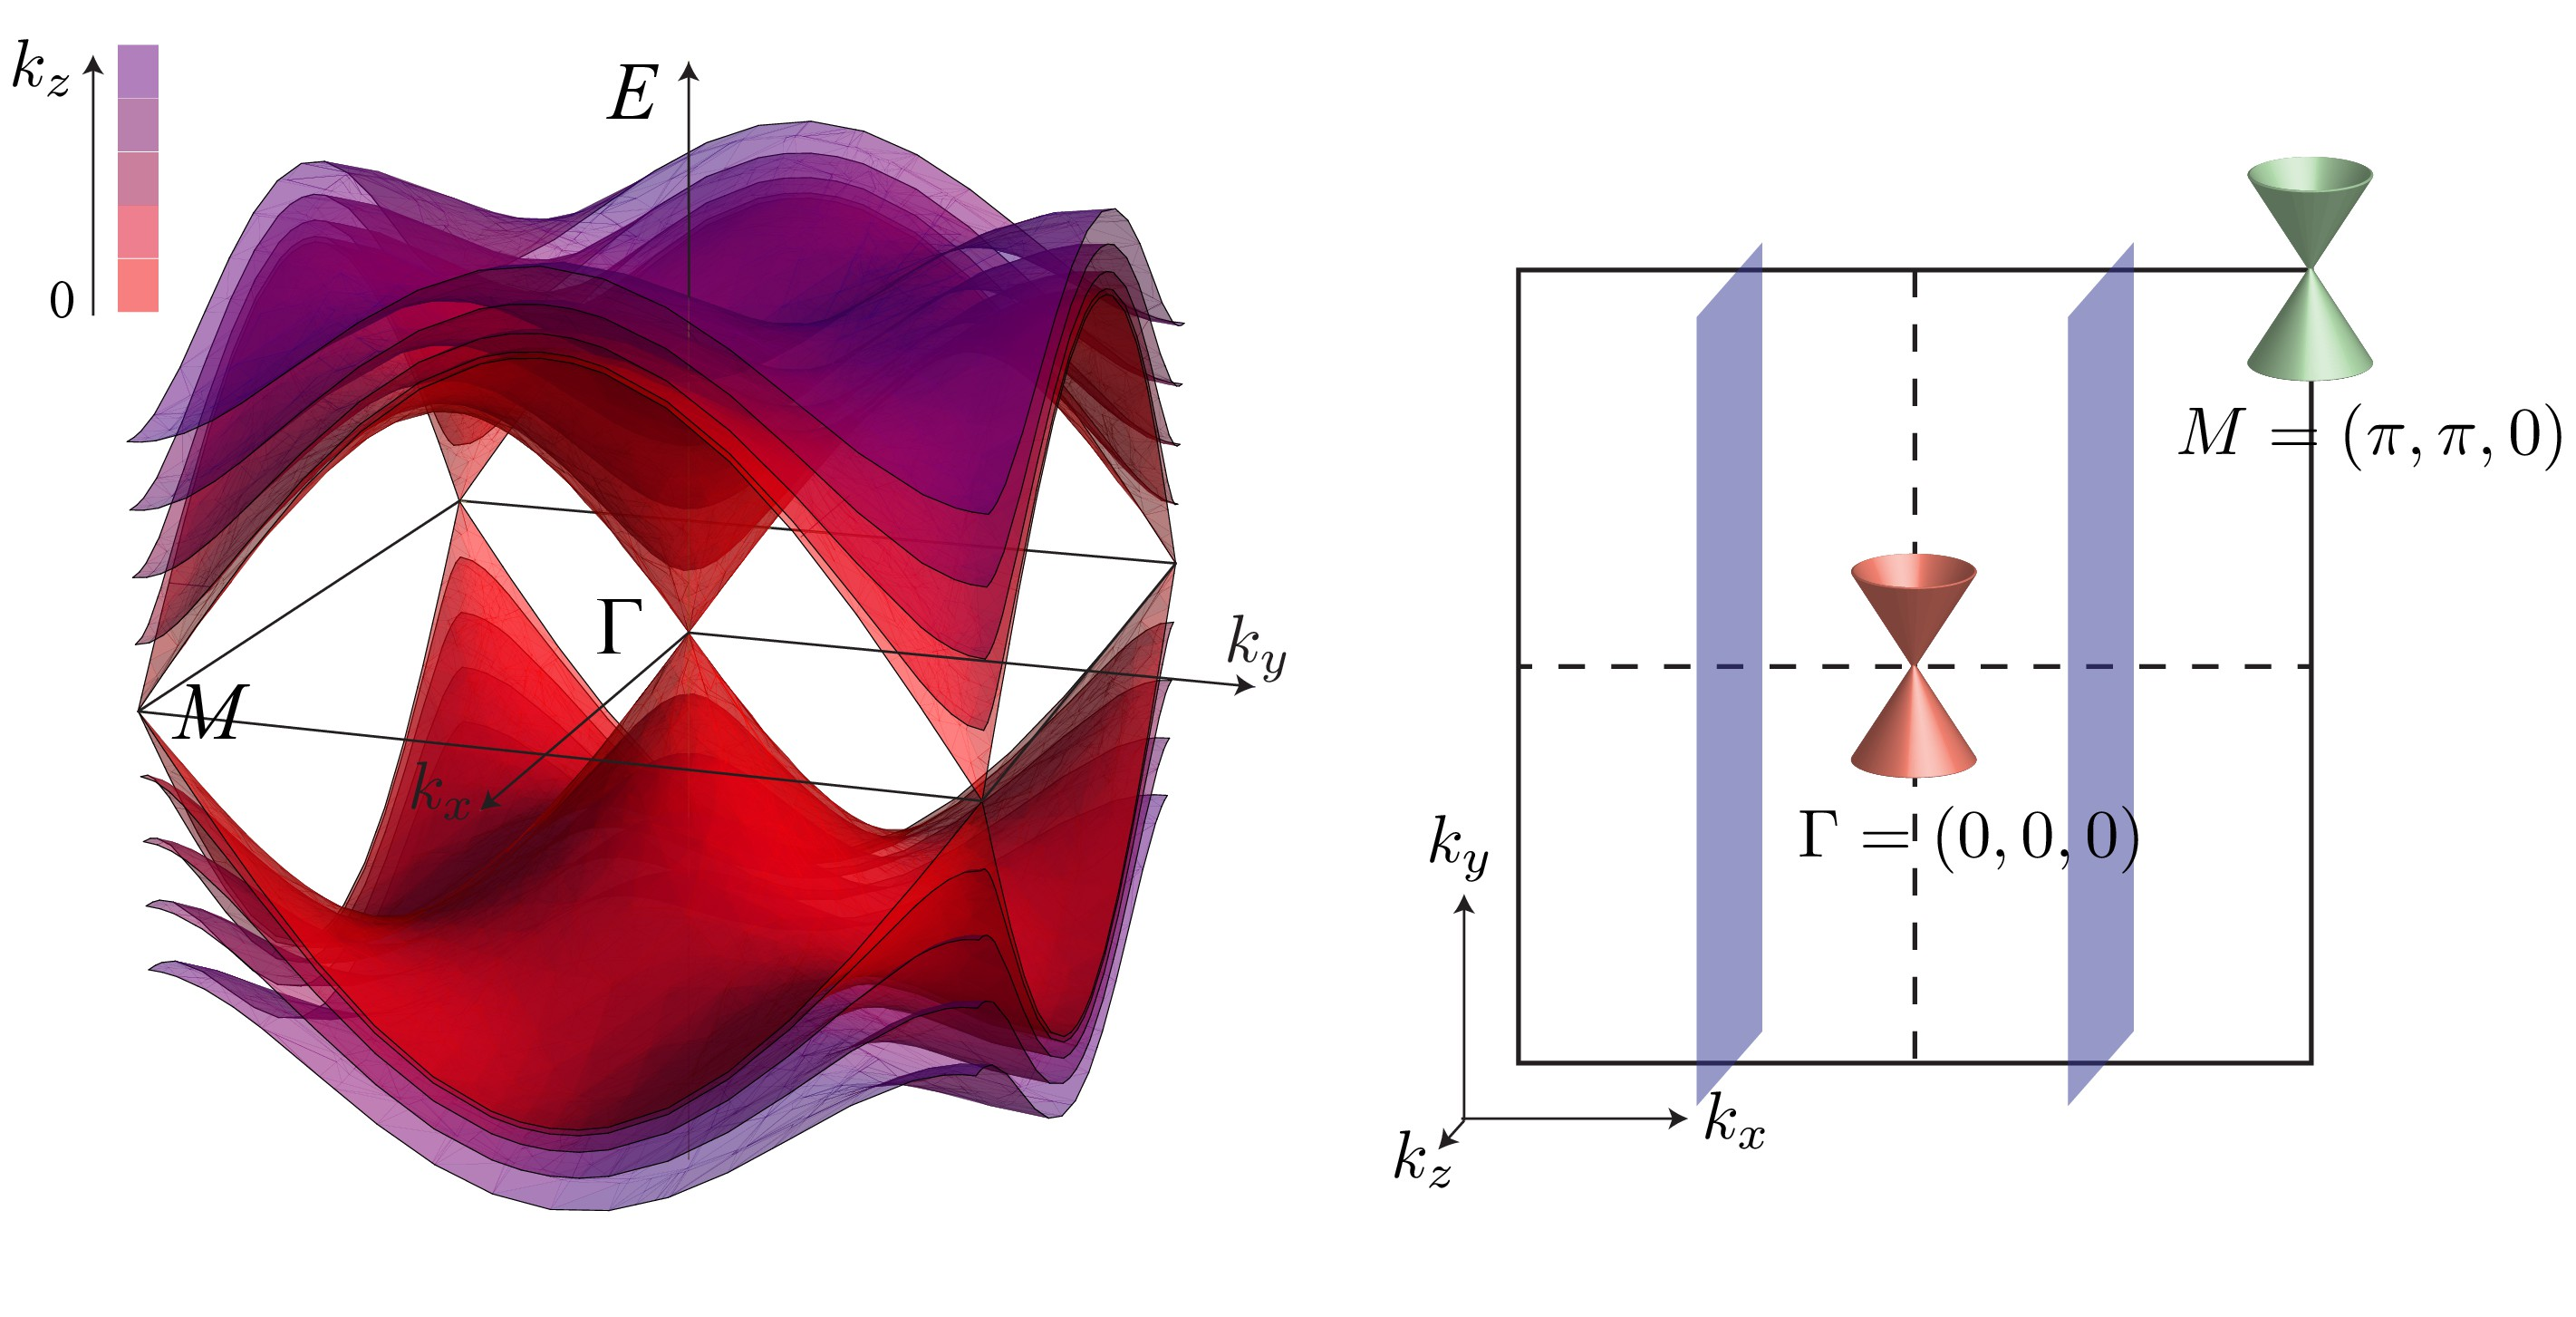
\includegraphics[width=0.9\textwidth]{Weylspectrumjpg.jpg}
	\caption{Energy spectrum of the coupled Dirac wire model \eqref{WeylTBHam}.}\label{fig:Weylspectrum}
\end{figure}

The energy spectrum of the two-band model is given by $E_\pm({\bf k})=\pm\sqrt{|g(k_x,k_y)|^2+\hbar^2\tilde{v}^2k_z^2}$ (see Fig.~\ref{fig:Weylspectrum}).
It gives two linearly dispersing Weyl cones of opposite chiralities in the \BZ centered at $K^+_0=\Gamma=(0,0,0)$ and $K^-_0=M=(\pi,\pi,0)$. Near these points, the Hamiltonians are of the linear form $H(K_0^\pm+\delta{\bf k})=\hbar\delta{\bf k}^TV^\pm\vec\sigma+O(\delta k^2)$, where $\vec\sigma=(\sigma_x,\sigma_y,\sigma_z)$ are Pauli matrices acting on the $(\psi^\odot,\psi^\otimes)$ degrees of freedom. The velocity matrices are \begin{align}\hbar V^\pm=\left(\begin{array}{ccc}-t_1&\pm t_2&0\\-t_1&\mp t_2&0\\0&0&\hbar\tilde{v}\end{array}\right),\end{align} whose determinant's %$\det(\hbar V)=\pm2\hbar\tilde{v}t_1t_2$ 
sign decides the $\pm$ chirality of the Weyl fermion at $\Gamma$ and $M$, i.e.~the $\pm1$ Fermi surface Chern invariants~\cite{WanVishwanathSavrasovPRB11,Ashvin_Weyl_review,RMP}. %Expanding about the two Weyl points and ignoring higher order terms gives $H(X^{\pm} + \delta {\mathbf{k}})= -t_1 (\delta k_x + \delta k_y) \sigma_x  \mp t_2 (\delta k_x - \delta k_y) \sigma_y  + v \delta k_z \sigma_z$.
The \AFTR symmetries \eqref{AFTR} in the single-body picture are expressed under Fourier transformation as \begin{gather}\mathcal{T}_{11}\vec\psi_{\bf k}\mathcal{T}_{11}^{-1}=T_{11}({\bf k})\vec\psi_{-\bf k},\quad\mathcal{T}_{\bar{1}1}\vec\psi_{\bf k}\mathcal{T}_{\bar{1}1}^{-1}=T_{\bar{1}1}({\bf k})\vec\psi_{-\bf k},\nonumber\\T_{11}({\bf k})=\left(\begin{array}{ccc}0&-e^{i(k_x+k_y)}\\1&0\end{array}\right)\mathcal{K},\nonumber\\T_{\bar{1}1}({\bf k})=\left(\begin{array}{ccc}0&-e^{ik_y}\\e^{-ik_x}&0\end{array}\right)\mathcal{K},\label{AFTRk}\end{gather} where $\mathcal{K}$ is the complex conjugation operator. They satisfy the appropriate algebraic relations \eqref{AFTRalg} in momentum space \begin{gather}T_{11}(-{\bf k})T_{\bar{1}1}({\bf k})=T_{\bar{1}1}(-{\bf k})T_{11}({\bf k})=-e^{-ik_y}\nonumber\\T_{11}(-{\bf k})T_{\bar{1}1}({\bf k})^{-1}=T_{\bar{1}1}(-{\bf k})^{-1}T_{11}({\bf k})=e^{-ik_x}\end{gather} and the coupled wire model \eqref{BlochHam} is \AFTR symmetric \begin{align}T_{11}({\bf k})H({\bf k})&=H(-{\bf k})T_{11}({\bf k}),\nonumber\\T_{\bar{1}1}({\bf k})H({\bf k})&=H(-{\bf k})T_{\bar{1}1}({\bf k}).\label{WeylTBT11}\end{align} The Weyl points are at time reversal invariant momenta (\hypertarget{TRIM}{TRIM}) $K^\pm_0\equiv-K^\pm_0$ (modulo the reciprocal lattice $2\pi\mathbb{Z}^2$), and the \AFTR operators $T_{11}(K^\pm_0)=-i\sigma_y\mathcal{K}$ and $T_{\bar{1}1}(K^\pm_0)=\mp i\sigma_y\mathcal{K}$ square to minus one. Hence the Weyl points are not only protected by the non-vanishing Fermi surface Chern invariant but also the Kramers' theorem. In addition, the model is also $C_2$ symmetric \begin{align}C_2({\bf k})H({\bf k})=H(C_2{\bf k})C_2({\bf k}) \,, \label{WeylTBC2}\end{align} where the twofold symmetry \eqref{C2} is represented in the single-body picture by a diagonal matrix \begin{align}\mathcal{C}_2\vec\psi_{\bf k}\mathcal{C}_2^{-1}=C_2({\bf k})\vec\psi_{C_2\bf k},\quad C_2({\bf k})=\left(\begin{array}{*{20}c}i&0\\0&-ie^{-i(k_x+k_y)}\end{array}\right)\label{C2k}\end{align} (suppressing the screw phase $e^{-ik_za/2}$ in the continuum limit $a\to0$). It agrees with the fermion statistics \eqref{C2square} $C_2(-k_x,-k_y,k_z)C_2(k_x,k_y,k_z)=-1$, and the algebraic relations \eqref{C2Trelation} with the \AFTR operators \begin{align}C_2(-{\bf k})T_{11}({\bf k})&=-T_{11}(C_2{\bf k})^{-1}C_2({\bf k})\nonumber\\C_2(-{\bf k})T_{\bar{1}1}({\bf k})&=-T_{\bar{1}1}(C_2{\bf k})^{-1}C_2({\bf k})\end{align} for $C_2{\bf k}=(-k_x,-k_y,k_z)$.

\subsection{The anomalous Dirac semimetal}\label{sec:anomaly}
We notice that the coupled wire Dirac model \eqref{WeylTBHam} and its massless energy spectrum in Fig.~\ref{fig:Weylspectrum} are anomalous with respect to the \AFTR symmetries $\mathcal{T}_{11}$ and $\mathcal{T}_{\bar{1}1}$ as well as the $C_2$ symmetry if it is proper symmorphic and not a screw rotation. This means that it cannot be realized in a single-body three dimensional lattice system with the \AFTR or $C_2$ symmetries. In a sense, it is not surprising at all since the chiral Dirac strings that constitute \eqref{WeylTBHam} are themselves violating fermion doubling~\cite{Nielsen_Ninomiya_1981,NielsenNinomiyaPLB1981}. Here we further elaborate on the anomalous Dirac spectrum (Fig.~\ref{fig:Weylspectrum}) where the pair of Weyl points are separately located at two \TRIM $K^\pm_0$. We also comment on the non-trivial consequence of the anomaly and pave the path for later discussion on many-body interactions.

We begin with two 2D planes in momentum space parallel to $k_yk_z$ located at $k_x=\pm\pi/2$. They are represented by the two blue planes in Fig.~\ref{fig:Weylspectrum}. The \AFTR or $C_2$ symmetries require the Chern invariants \begin{align}\mathrm{Ch}_1=\frac{i}{2\pi}\int\mathrm{Tr}(P\partial_{k_y}P\partial_{k_z}P)dk_ydk_z\label{1stChern}\end{align} at $k_x=\pm\pi/2$ to be opposite, where $P({\bf k})=(1-H({\bf k})/|E({\bf k})|)/2$ is the projection operator onto the negative energy band. This is because the \AFTR symmetry is anti-unitary and preserves the orientation of the $k_yk_z$ plane, whereas $C_2$ is unitary but reverses the orientation of the $k_yk_z$ plane. (See appendix~\ref{sec:Chernapp} for a detailed proof.) On the other hand, the two Chern invariants along the two planes must differ by 1 because they sandwich a single Weyl point at $\Gamma$. This forces the Chern invariants to be a half integer $\mathrm{Ch}_1=\pm1/2$, which is anomalous.

While the $C_2$ anomaly can be resolved simply by doubling the unit cell and assuming it originates from a microscopic non-symmorphic screw axis, the \AFTR anomaly is stronger because the two antiferromagnetic combinations \eqref{AFTRalg} generate lattice translations and fix the unit cell size. There are three resolutions. \begin{enumerate}\item The \AFTR symmetries are broken by high energy degrees of freedom when $k_z$ is large. \item The spectrum in Fig.~\ref{fig:Weylspectrum} is the holographic 3D boundary spectrum of an \AFTR symmetric weak topological insulator in 4D. \item The spectrum is generated by strong many-body interaction non-holographically in 3D.\end{enumerate} Below we discuss the first two resolutions, and we leave the many-body interaction-enabled situation to Sec.~\ref{sec:intenable}.

\subsubsection{Broken symmetries and coarse-graining}\label{sec:brokensymmetry}
The mapping between the original Dirac fermion model and the emergent Dirac fermion model from a coupled-wire construction can be qualitatively understood as a coarse-graining procedure. Here, the high-energy microscopic electronic degrees of freedom are integrated out. The procedure can be repeated indefinitely and resembles a real-space renormalization. For example, the gapless Dirac electronic structure of the coupled wire model can acquire a finite mass by symmetry-breaking dimerizations. These dimerizations can be arranged in a topological manner that spatially wind non-trivially around a collective vortex. These second-stage vortices can subsequently be assembled into an array similar to the previous construction except now with a longer lattice constant. The system again recovers a massless Dirac spectrum under inter-vortex electron tunneling in low-energy and long length scale. The mapping therefore establishes an equivalence between the continuous isotropic massless Dirac fermion and the semi-discrete anisotropic coupled Dirac wire model.

In the present case when the chiral Dirac channels originate from vortex strings in an underlying microscopic Dirac insulator, the spatial modulation of mass parameters $m({\bf r})$ actually violate one of the \AFTR symmetries, $m({\bf r})^\ast\neq m({\bf r}+({\bf e}_x\pm{\bf e}_y)/2)$, where $\ast$ stands for complex conjugation. For instance, since all elliptic functions must contain at least two zeros and two poles in its periodic cell, the Jacobian elliptic mass function \eqref{Jacobielliptic} has longer periods than ${\bf e}_x$ and ${\bf e}_y$ in Fig.~\ref{fig:WeylTB}, and thus must break $\mathcal{T}_{11}$ or $\mathcal{T}_{\bar{1}1}$. The symmetry is broken only in the ultra-violet limit at large $k_z$ where the chiral Dirac line nodes meet the microscopic bulk band (see Fig.~\ref{fig:Diracstring}) at high energy $\sim|m({\bf r})|$. In fact, the above anomalous argument shows that {\em all} mass parameter configurations that produce the 3D vortex lattice array (Fig.~\ref{fig:vortexlattice}) must either (a) break both the \AFTR symmetries $\mathcal{T}_{11}$ and $\mathcal{T}_{\bar{1}1}$, or (b) preserve one but violate translation so that the unit cell is enlarged and the two Weyl points collapse onto each other in momentum space. (See Figs.~\ref{fig:Chernstack} and \ref{fig:DiracTB}.)

For instance, the microscopic system can be connected to a stack of Chern insulating ribbons (or lowest Landau levels) with alternating chiralities shown in Fig.~\ref{fig:Chernstack}. Instead of being supported by vortices of Dirac mass, the chiral Dirac wires are now realized as edge modes of Chern insulating strips. Each 2D ribbon (represented by thick dashed dark blue lines) is elongated in the out-of-paper $z$-direction but is finite along the $(110)$ direction and holds counter-propagating boundary chiral Dirac channels. The dark blue arrows represent the orientations of the Chern ribbons that accommodate the boundary Dirac channels with the appropriate propagating directions. Here the Chern ribbon pattern in Fig.~\ref{fig:Chernstack}(a) breaks both \AFTR axes. The pattern in Fig.~\ref{fig:Chernstack}(b) preserves $\mathcal{T}_{\bar{1}1}$. However, translation symmetry is also broken and the coupled Dirac wire model now has an enlarged unit cell (light blue dashed boxes) that consists of two pairs of counter-propagating chiral Dirac channels. All Chern ribbon patterns must break the $C_2$ symmetry about a Dirac wire because each wire is connected to one and only one Chern ribbon in a particular direction.

\begin{figure}[htbp]
	\centering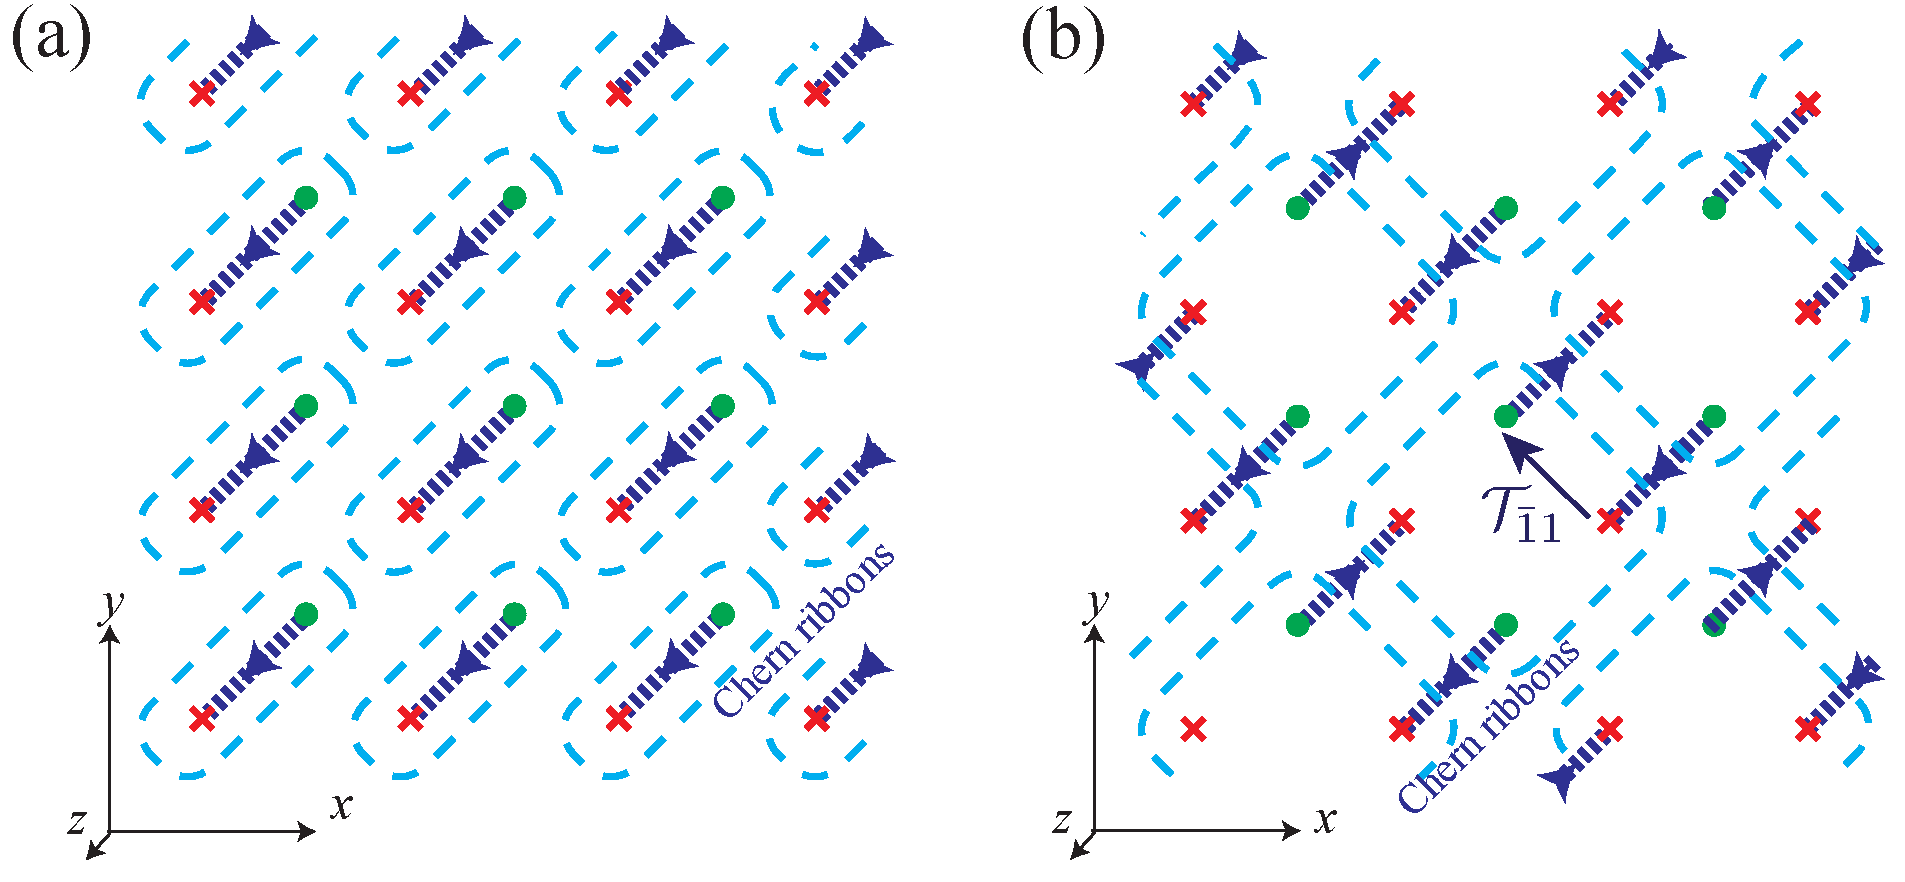
\includegraphics[width=0.9\textwidth]{Chernstack}
	\caption[Chiral Dirac channels realized on the edge of Chern insulating ribbons.]{Chiral Dirac channels ({\color{red}$\boldsymbol\times$} and {\color{green}$\bullet$}) realized on the edge of Chern insulating ribbons (dark blue directed lines) stacked along the $(\bar{1}10)$ normal direction.}\label{fig:Chernstack}
\end{figure}

Now we go back to the vortex lattice generated by the Jacobian elliptic Dirac mass function $m({\bf r})$ in \eqref{Jacobielliptic} and consider its symmetries. For this purpose, we use the symmetry properties of the (rescaled) Jacobian elliptic function~\cite{ReinhardtWalker10} \begin{align}&\mathrm{sd}(x+iy)=-\mathrm{sd}(x+1+iy)=-\mathrm{sd}(x+iy+i)\nonumber \,, \\&\mathrm{sd}\left(x+iy+\frac{1+i}{2}\right)=-i\frac{C}{\mathrm{sd}(x+iy)}\label{sdprop} \,, \\&\mathrm{sd}(-x-iy)=-\mathrm{sd}(x+iy)\nonumber \,,\end{align} where $C$ is some unimportant real constant that depends on the modulus of $\mathrm{sd}$ and will never appear in the mass function $m({\bf r})=m_0\mathrm{sd}(x+iy)/|\mathrm{sd}(x+iy)|$. We see from the minus sign in the first equation that the Jacobian elliptic function, and consequently the mass function, have primitive periods ${\bf e}_x\pm{\bf e}_y$ and therefore have a unit cell of size 2 (see Fig.~\ref{fig:DiracTB}(a)). Choosing $m_0=|m_0|e^{i\pi/4}$, we see from the second equation that $\mathcal{T}_{11}$ (or $\mathcal{T}_{\bar{1}1}$) is preserved (resp.~broken) \begin{align}m\left({\bf r}+\frac{{\bf e}_x\pm{\bf e}_y}{2}\right)=\pm m({\bf r})^\ast,\label{massT11}\end{align} and thus the parent Dirac Hamiltonian \eqref{DiracHam} is $\mathcal{T}_{11}$-symmetric \begin{align}\hat{T}H_{\mathrm{Dirac}}\left(-{\bf k},{\bf r}+\frac{{\bf e}_x+{\bf e}_y}{2}\right)\hat{T}^{-1}=H_{\mathrm{Dirac}}({\bf k},{\bf r}),\end{align} for $\hat{T}=is_y\mathcal{K}$. Lastly, the third property of \eqref{sdprop} entails the mass function $m({\bf r})=-m(C_2{\bf r})$ is odd under $C_2$, and consequently the parent Dirac Hamiltonian is (screw) rotation symmetric \begin{align}\hat{C}_2H_{\mathrm{Dirac}}(C_2{\bf k},C_2{\bf r})\hat{C}_2^{-1}=H_{\mathrm{Dirac}}({\bf k},{\bf r}),\label{massC2}\end{align} where $\hat{C}_2=is_z\mu_z$ (or microscopically $e^{-ik_za/2}is_z\mu_z$) anticommuting with the mass terms $m_1\mu_x+m_2\mu_y$ in $H_{\mathrm{Dirac}}$ (see \eqref{DiracHam}), and $C_2{\bf k}=(-k_x,-k_y,k_z)$, $C_2{\bf r}=(-x,-y,z)$.

\begin{figure}[htbp]
	\centering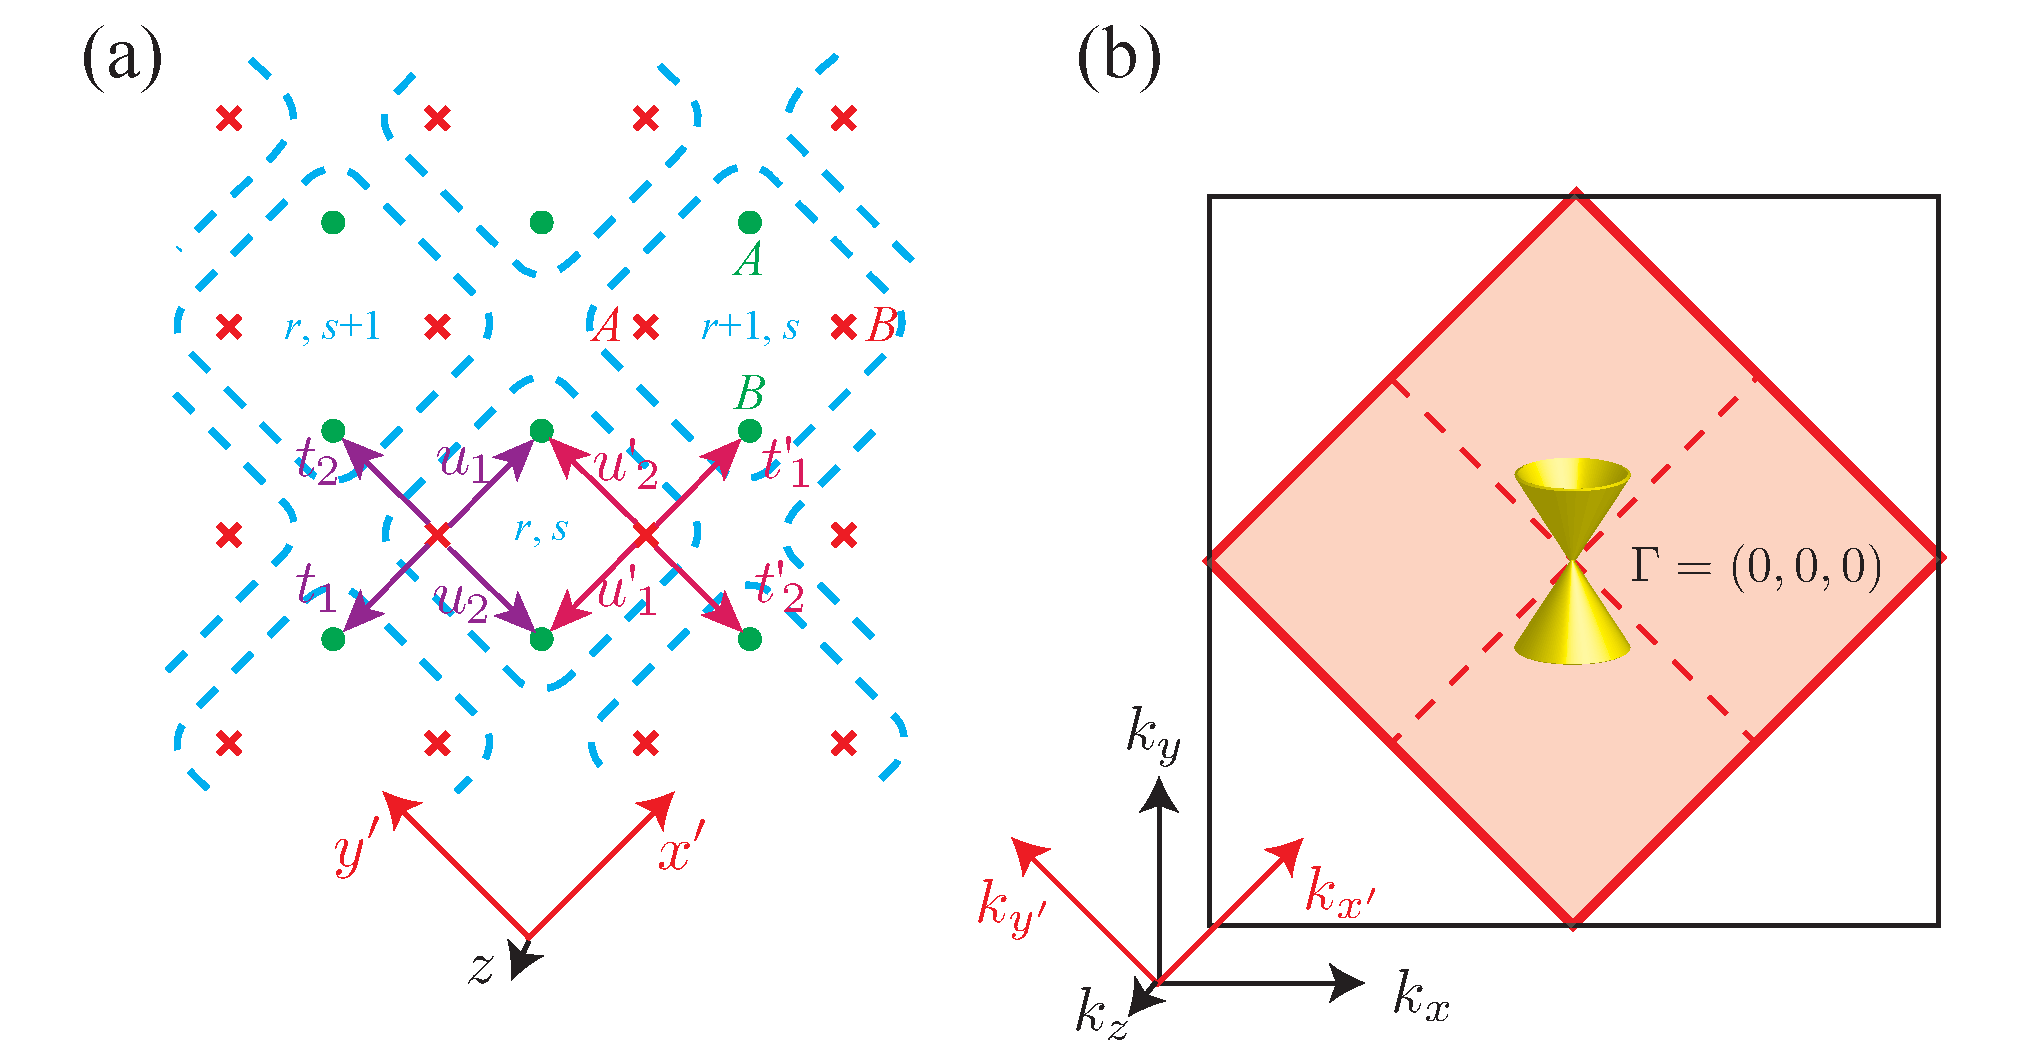
\includegraphics[width=0.9\textwidth]{DiracTB}
	\caption[(a) The massive AFTR and $C_2$ breaking coupled Dirac wire model. (b) The reduced Brillouin zone (BZ).]{(a) The massive AFTR and $C_2$ breaking coupled Dirac wire model. (b) The reduced Brillouin zone (BZ) after translation symmetry breaking where the two Weyl points collapse to a single Dirac point at $M$.}\label{fig:DiracTB}
	\centering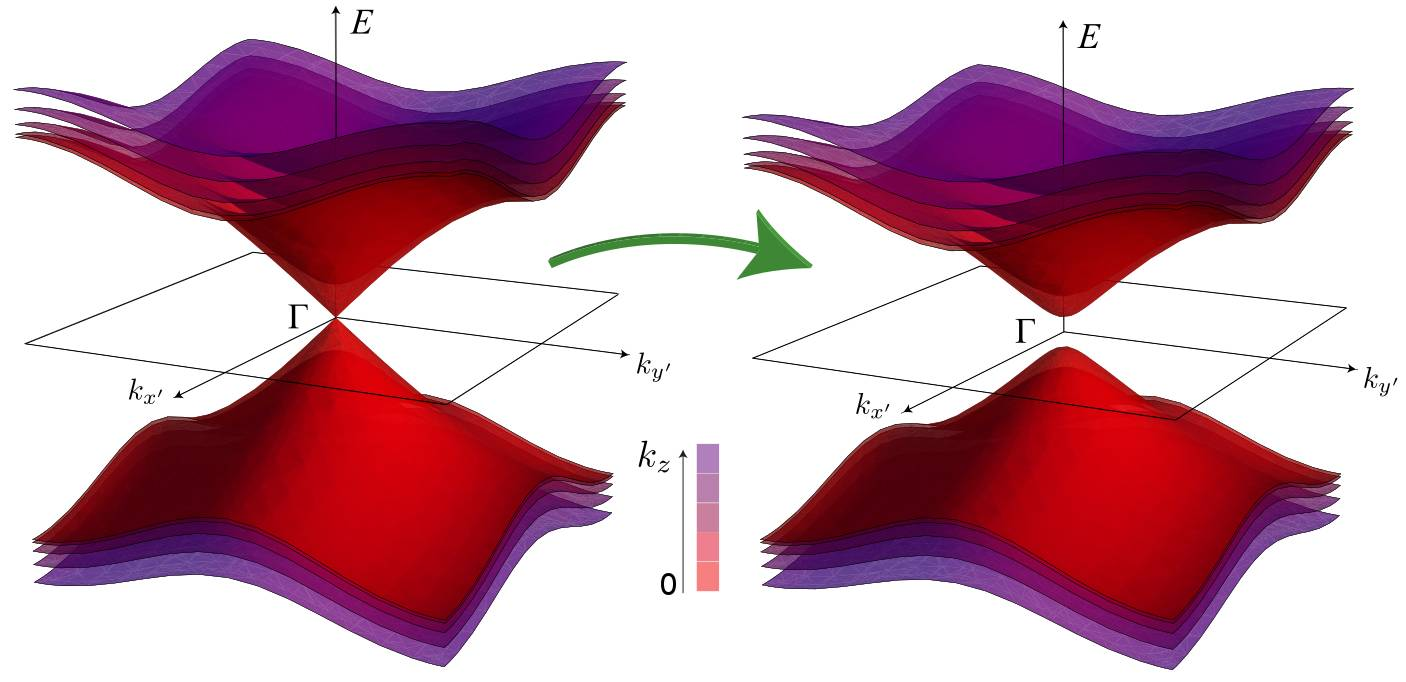
\includegraphics[width=0.96\textwidth]{Diracmassjpg.jpg}
	\caption{Dirac mass gap $2|\Delta|$ introduced by AFTR and $C_2$ symmetry breaking dimerization $\Delta=\Delta_1+i\Delta_2$.}\label{fig:Diracmassjpg}
\end{figure}

Remembering that the coupled wire model \eqref{WeylTBHam} (Fig.~\ref{fig:WeylTB}) descended from a vortex lattice of the microscopic parent Dirac Hamiltonian \eqref{DiracHam}, the Dirac mass $m({\bf r})$ actually allows the model to carry fewer symmetries than the low-energy effective Hamiltonian \eqref{WeylTBHam} suggests. Now that the translation symmetry is lowered, the \BZ is reduced (see Fig.~\ref{fig:DiracTB}(b)) so that the two Weyl points now coincide at the origin $\Gamma$. This recovers an unanomalous Dirac semimetallic model \eqref{DiracHam0} around $(k_{x'},k_{y'})=(0,0)$. The fourfold degenerate Dirac point is protected and pinned at $\Gamma$ due to the remaining \AFTR symmetry $\mathcal{T}_{11}$ -- which takes the role of a spinful time reversal ($\hat{T}^2=-1$) in the continuum limit -- and the $C_2$ (screw) symmetry about the $z$-axis. However, if any of these symmetries is further broken, the fourfold degeneracy of the Dirac point is not protected (c.f.~the original continuum Dirac model \eqref{DiracHam}). Figure~\ref{fig:DiracTB}(a) shows a dimerized coupled Dirac wire model that introduces a finite mass for the Dirac fermion. We label the Dirac fermion operators as $\psi_{r,s}^{\mu,\sigma}$, for $\sigma=\odot,\otimes$ the chirality, $\mu=A,B$ the new sublattice label, and $(r,s)$ label the coordinates of the unit cell according to the $45^\circ$-rotated $x',y'$-axes. \begin{align}\mathcal{H}'=&\sum_{r,s}\sum_{\mu=A,B}\hbar\tilde{v}\left({\psi_{r,s}^{\mu,\odot}}^\dagger k_z\psi_{r,s}^{\mu,\odot}-{\psi_{r,s}^{\mu,\otimes}}^\dagger k_z\psi_{r,s}^{\mu,\otimes}\right)\nonumber\\&+iu_1{\psi_{r,s}^{A,\odot}}^\dagger\psi_{r,s}^{A,\otimes}-iu'_1{\psi_{r,s}^{B,\odot}}^\dagger\psi_{r,s}^{B,\otimes}+h.c.\nonumber\\&-u_2{\psi_{r,s}^{B,\odot}}^\dagger\psi_{r,s}^{A,\otimes}+u'_2{\psi_{r,s}^{A,\odot}}^\dagger\psi_{r,s}^{B,\otimes}+h.c.\label{DiracTBHam}\\&-it_1{\psi_{r-1,s}^{A,\odot}}^\dagger\psi_{r,s}^{A,\otimes}+it'_1{\psi_{r+1,s}^{B,\odot}}^\dagger\psi_{r,s}^{B,\otimes}+h.c.\nonumber\\&+t_2{\psi_{r,s+1}^{B,\odot}}^\dagger\psi_{r,s}^{A,\otimes}-t'_2{\psi_{r,s-1}^{A,\odot}}^\dagger\psi_{r,s}^{B,\otimes}+h.c.\nonumber \,.\end{align} For instance, the model is identical to the \AFTR and $C_2$ symmetric one in \eqref{WeylTBHam} when $t_j=t'_j=u_j=u'_j$ for $j=1,2$. However, when the symmetries are broken, these hopping parameters do not have to agree.

The Bloch band Hamiltonian after Fourier transformation is \begin{gather}H({\bf k})=\left(\begin{array}{*{20}c}\hbar\tilde{v}k_z&h(k_{x'},k_{y'})\\h(k_{x'},k_{y'})^\dagger&-\hbar\tilde{v}k_z\end{array}\right),\label{DiracBloch}\\h(k_{x'},k_{y'})=\left(\begin{array}{*{20}c}iu_1-it_1e^{-ik_{x'}}&u'_2-t'_2e^{-ik_{y'}}\\-u_2+t_2e^{ik_{y'}}&-iu'_1+it'_1e^{ik_{x'}}\end{array}\right)\nonumber \,, \end{gather} where the $2\times2$ identity matrix and $h(k_{x'},k_{y'})$ acts on the sublattice $\mu=A,B$ degrees of freedom, and $-\pi\leq k_{x'},k_{y'}\leq\pi$ are the rotated momenta. We perturb about the Dirac fixed point by introducing the dimerizations $\Delta_j$ \begin{align}t_j=t'_j=u_j-\Delta_j=u'_j-\Delta_j\end{align} for $j=1,2$. About the $\Gamma=(0,0,0)$ point, \begin{align}H(\Gamma+\delta{\bf k})=&\hbar\tilde{v}\delta k_z\sigma_z-t_1\delta k_{x'}\sigma_x-t_2\delta k_{y'}\sigma_y\mu_x\nonumber\\&-\Delta_1\sigma_y\mu_z+\Delta_2\sigma_y\mu_y+O(\delta k^2).\label{DiracHamwire}\end{align} See Fig.~\ref{fig:Diracmassjpg} for its massive spectrum.

\begin{figure}[htbp]
	\centering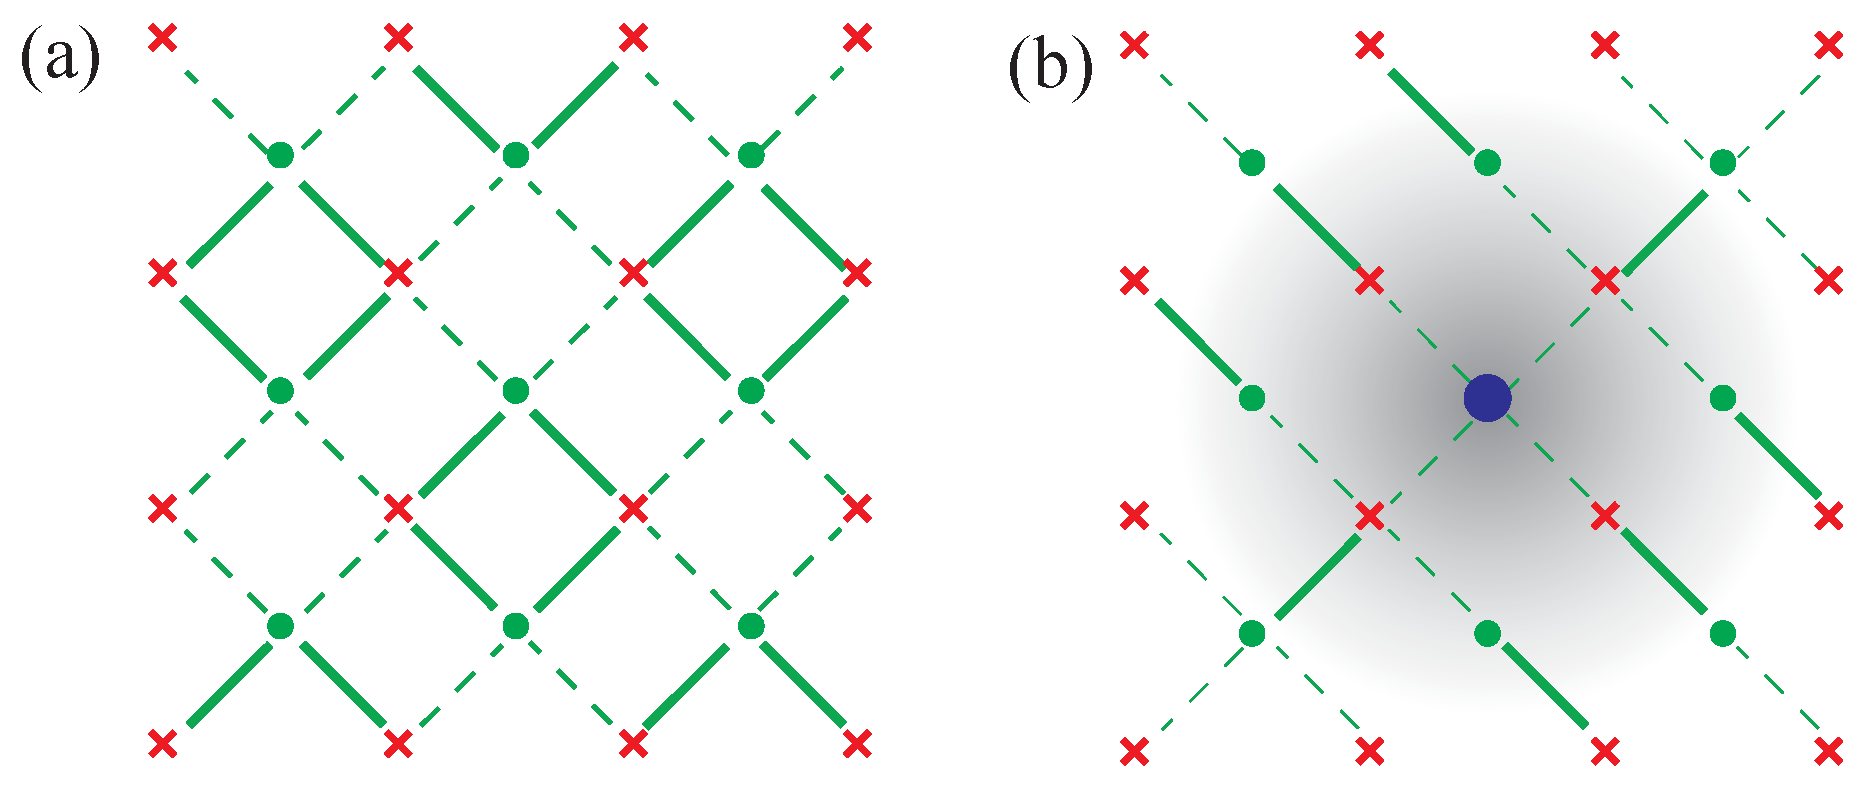
\includegraphics[width=0.8\textwidth]{dimerization}
	\caption[(a) Dimerized model of a massive Dirac fermion. (b) Vortex of dimerizations.]{(a) Dimerized model of a massive Dirac fermion. (b) Vortex of dimerizations $\Delta=\Delta_1+i\Delta_2$ that leaves behind a massless localized chiral Dirac channel (blue dot).}\label{fig:dimerization}
\end{figure}

Here the \AFTR symmetry $\mathcal{T}_{11}$ and the twofold rotation $\mathcal{C}_2$ are represented in the single-body picture by \begin{align}T_{11}({\bf k})&=\left(\begin{smallmatrix}0&0&-e^{ik_x}&0\\0&0&0&-1\\1&0&0&0\\0&e^{ik_x}&0&0\end{smallmatrix}\right)\mathcal{K},\nonumber\\C_2({\bf k})&=\left(\begin{smallmatrix}i&0&0&0\\0&ie^{-i(k_x+k_y)}&0&0\\0&0&-ie^{-ik_x}&0\\0&0&0&-ie^{-ik_y}\end{smallmatrix}\right)\end{align} (again suppressing the $C_2$ screw phase $e^{-ik_za/2}$ in the continuum limit $a\to0$). In the small $k_x,k_y$-limit, $T_{11}(0)=-i\sigma_y\mathcal{K}$ and $C_2(0)=i\sigma_z$. It is straightforward to check that the dimerization $\Delta_2$ preserves $\mathcal{T}_{11}$ while both $\Delta_1,\Delta_2$ breaks $C_2$.

Since the coupled wire model \eqref{DiracHamwire} and the parent continuum Dirac model \eqref{DiracHam} have the same matrix and symmetry structure, we can apply the same construction we discussed before to the new coarse-grained model \eqref{DiracHamwire}. For instance, the non-competing dimerizations $\Delta({\bf r})=\Delta_1({\bf r})+i\Delta_2({\bf r})$ can spatially modulate and form vortices in a longer length scale. Figure~\ref{fig:dimerization}(b) shows a dimerization pattern that corresponds to a single vortex in $\Delta$. The solid (dashed) lines represent strong (resp.~weak) backscattering amplitudes. In the fully dimerized limit where the dashed bonds vanish, all Dirac channels are gapped except the one at the center (showed as a blue dot). In the weakly dimerized case, there is a collective chiral Dirac channel whose wave function is a superposition of the original channels and is exponentially localized at the $\Delta$-vortex core, but now with a length scale longer than that of the original $m$-vortex lattice. These collective chiral Dirac $\Delta$-vortices can themselves form a coupled array, like \eqref{WeylTBHam}, and give a Dirac semimetal of even longer length scale. The single-body coupled vortex construction is therefore a coarse-graining procedure that recovers equivalent emergent symmetries at each step. \begin{align}\begin{diagram}\mbox{Dirac semimetal}&\pile{\rTo^{\mbox{\small mass vortices}}\\\lTo_{\mbox{\small coupled wire model}}}&\mbox{chiral Dirac strings \,.}\end{diagram}\end{align}

\subsubsection{Holographic projection from 4D}\label{sec:holproj4D}
The coupled wire model \eqref{WeylTBHam} with two \AFTR axes can be supported by a weak topological insulator (\hypertarget{WTI}{WTI}) in four dimensions. Instead of realizing the chiral Dirac channels using mass vortices of a 3D Dirac semimetal, they can be generated as edge modes along the boundaries of 2D Chern insulators (or lowest Landau levels). The 4D \WTI is constructed by stacking layers of Chern insulators parallel to the $zw$-plane along the $x$ and $y$ directions. The Chern layers $L_{\bf r}$, labeled by the checkerboard lattice vector ${\bf r}=r_x{\bf e}_x+r_y{\bf e}_y$ on the $xy$-plane, have alternating orientations so that $\mathrm{Ch}[L_{\bf r}]=1$ if $r_x,r_y$ are integers and $\mathrm{Ch}[L_{\bf r}]=-1$ if $r_x,r_y$ are half-integers.  The model therefore carries both \AFTR symmetries $\mathcal{T}_{11}$ and $\mathcal{T}_{\bar{1}1}$ as well as the $C_2$ rotation about $zw$, and when cleaved along a 3D hyper-surface normal to $w$, it generates the array of alternating chiral Dirac channels in Fig.~\ref{fig:WeylTB}.

The 4D \WTI model can also be regarded as a stack of 3D antiferromagnetic topological insulators (\hypertarget{AFTI}{AFTI})~\cite{MongEssinMoore10}. Restricting to the 3D hyperplane normal to $-{\bf e}_x+{\bf e}_y$, this model consists of alternating Chern insulating layers parallel to the $wz$-plane stacked along the ${\bf e}_x+{\bf e}_y$ direction. This 3D model describes an \AFTI with a non-trivial $\mathbb{Z}_2$ index. For instance along the boundary surfaces normal to $w$ or $z$ that preserve the antiferromagnetic symmetry $\mathcal{T}_{11}$, the model leaves behind a 2D array of alternating chiral Dirac wires. The uniform nearest wire backscattering term $t_1$ (see \eqref{WeylTBHam}) introduces a linear dispersion along the $11$-direction and gives rise to a single massless surface Dirac cone spectrum at a \TRIM on the boundary of the surface \BZ where $\mathcal{T}_{11}^2=-1$. The 4D \WTI model is identical to stacking these 3D \AFTI along the $\bar{1}1$-off-diagonal direction $-{\bf e}_x+{\bf e}_y$. 

\subsection{Surface Fermi arcs}\label{sec:fermiarc1}

\subsubsection{AFTR breaking surfaces}\label{sec:fermiarcAFTRbreaking}

\begin{figure}[htbp]
	\centering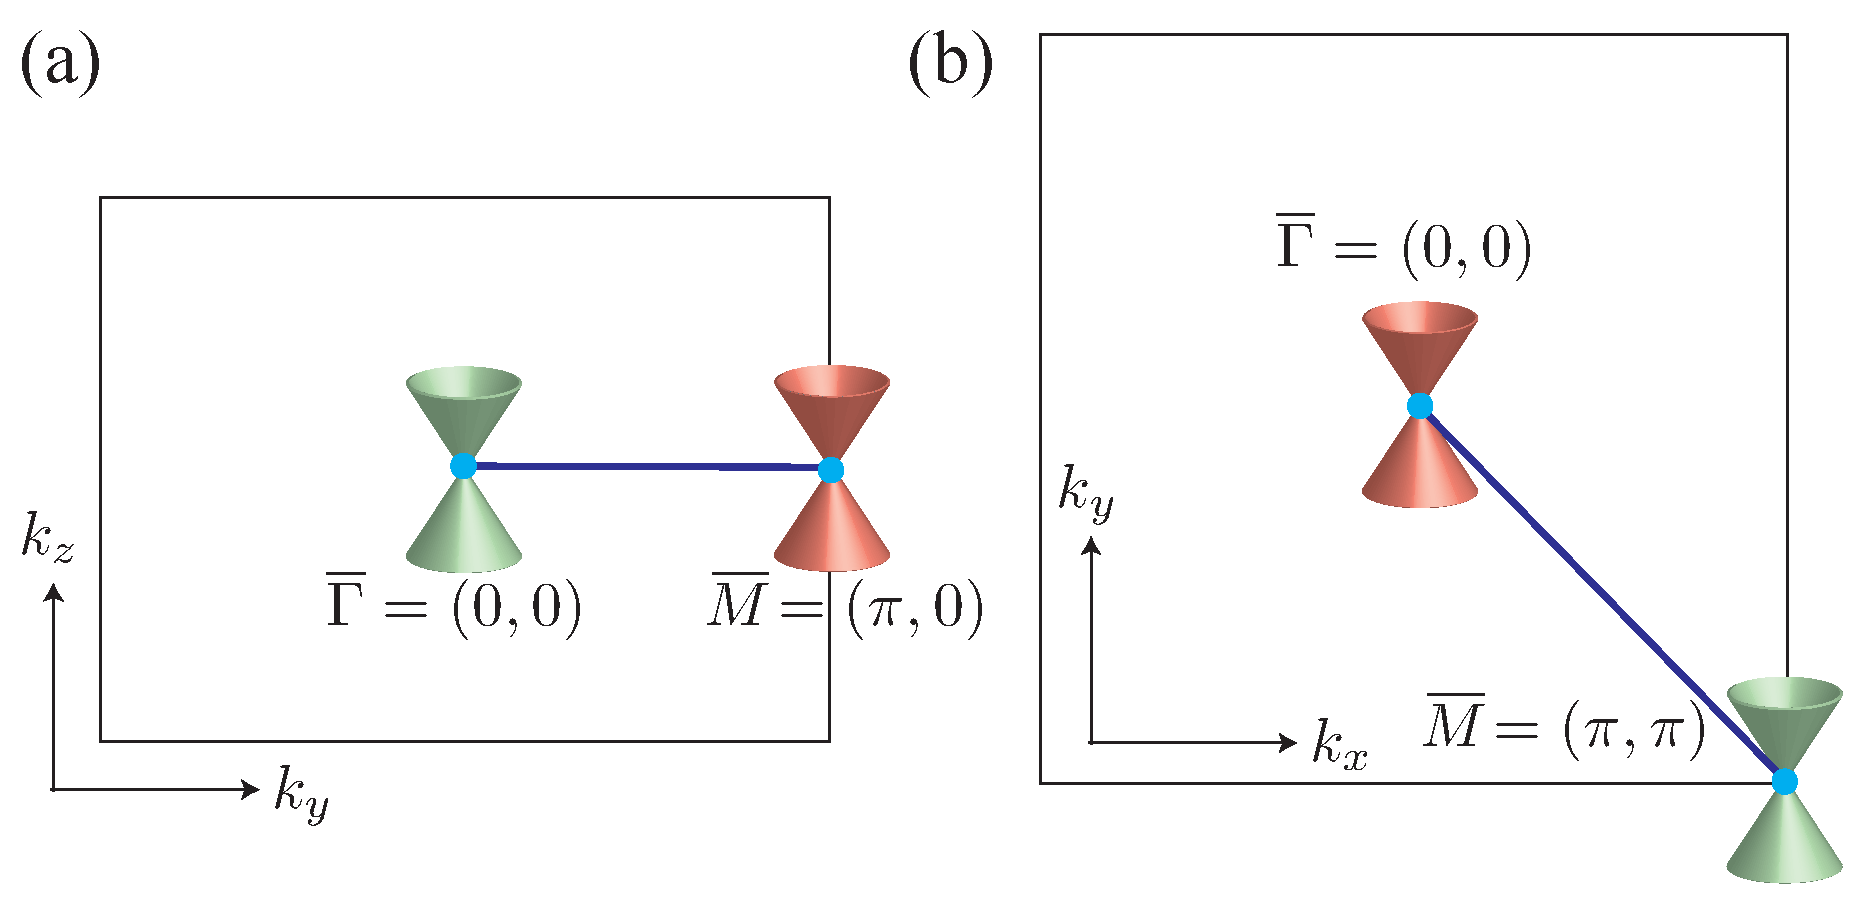
\includegraphics[width=0.8\textwidth]{fermiarc1}
	\caption[Fermi arcs joining projected Weyl points on the surface Brillouin zones]{Fermi arcs (blue lines) joining projected Weyl points on the surface Brillouin zones along (a) the $(100)$ surface and (b) the $(001)$ surface.}\label{fig:fermiarc1}
\end{figure}
We discuss the surface states of the coupled Dirac wire model \eqref{WeylTBHam}. Similar to the boundary surface of a translation symmetry protected Dirac semimetal (or more commonly called a Weyl semimetal), there are Fermi arcs connecting the surface-projected Weyl points~\cite{WanVishwanathSavrasovPRB11,Ashvin_Weyl_review,RMP}. First we consider the $(100)$ surface normal to $x$-axis (see Fig.~\ref{fig:WeylTB}). We assume the boundary cuts between unit cells and set the Fermi energy at $\varepsilon_f=0$. At $k_z=0$ and given a fixed $k_y\in(-\pi,\pi)$, the tight-binding model \eqref{BlochHam} is equivalent to the Su-Schriffer-Heeger model~\cite{SSH} or a 1D class AIII topological insulator~\cite{SchnyderRyuFurusakiLudwig08,Kitaevtable08} along the $x$-direction protected by the chiral symmetry $\sigma_zH(k_x)=-H(k_x)\sigma_z$. It is characterized by the winding number \begin{align}w(k_y)&=\frac{i}{2\pi}\int_{-\pi}^\pi \frac{1}{g(k_x,k_y)}\frac{\partial g(k_x,k_y)}{\partial k_x}dk_x \,, \\&=\left(1+\mathrm{sgn}(k_y t_1/t_2)\right)/2.\nonumber\end{align} When $t_1,t_2$ have the same (or opposite) sign, the quasi-1D model is topological along the positive (resp.~negative) $k_y$-axis and thus carries a boundary zero mode. This corresponds to the Fermi line joining the two surface projected Weyl points at $\overline{\Gamma}$ and $\overline{M}$ (see Fig.~\ref{fig:fermiarc1}(a)). As the zero modes have a fixed chirality according to $\sigma_z$, they propagate uni-directionally with the dispersion $E(k_z)=\hbar\tilde{v}k_z\sigma_z$. The cleaving surface breaks \AFTR and $C_2$ symmetries, and so does the Fermi arc in Fig.~\ref{fig:fermiarc1}(a). For instance, any one of the \AFTR symmetries maps the boundary surface to an inequivalent one that cuts through unit cells instead of between them. As a result, the Fermi arc will connect the Weyl points along the opposite side of the $k_y$-axis for this surface. 

The $(010)$ surface Fermi arc structure is qualitatively equivalent to that of the $(100)$ surface. The $(110)$ and $(1\bar{1}0)$ surfaces that cleave along the diagonal and off-diagonal axes (see Fig.~\ref{fig:WeylTB}) respectively preserve the \AFTR symmetries $\mathcal{T}_{11}$ and $\mathcal{T}_{\bar{1}1}$. There are no protected surface Fermi arcs because the two bulk Weyl points project onto the same point on the surface Brillouin zone. Lastly, we consider the $(001)$ surface normal to the $z$-axis, which is the direction of the chiral Dirac strings that constitute the coupled wire model. A chiral Dirac channel cannot terminate on the boundary surface. In a single-body theory, it must bend and connect with an adjacent counter-propagating one. Although the $(001)$ plane is closed under the $C_2$ as well as both the \AFTR symmetries, the surface bending of Dirac channels must violate at least one of them. Here we consider the simplest case where the counter-propagating pair of Dirac channels within a unit cell re-connects on the boundary surface. This boundary is equivalent to a domain wall interface separating the Dirac semimetal \eqref{WeylTBHam} from an insulator where Dirac channels backscatters to their counter-propagating partner within the same unit cell. 

The domain wall Hamiltonian takes the form of a differential operator
\begin{align}\hat{\mathcal{H}}=&\sum_{m,j}-i\hbar\tilde{v}\left({\psi_{m,j}^\odot}^\dagger\partial_z\psi_{m,j}^\odot-{\psi_{m,j}^\otimes}^\dagger\partial_z\psi_{m,j}^\otimes\right)\label{WeylTBHamwall}\\&+it_1\left({\psi_{m,j}^\odot}^\dagger\psi_{m,j}^\otimes+\theta(z){\psi_{m-1,j-1}^\odot}^\dagger\psi_{m,j}^\otimes\right)+h.c.\nonumber\\&+t_2\theta(z)\left({\psi_{m-1,j}^\odot}^\dagger\psi_{m,j}^\otimes+{\psi_{m,j-1}^\odot}^\dagger\psi_{m,j}^\otimes\right)+h.c.\nonumber\end{align} by replacing $k_z\leftrightarrow-i\partial_z$ in \eqref{WeylTBHam}. Here $\theta(z)$ can be the unit step function or any function that asymptotically approaches 1 for $z\to\infty$ or 0 for $z\to-\infty$. The model therefore describes the Dirac semimetal \eqref{WeylTBHam} for positive $z$, and an insulator for negative $z$ where Dirac channels are pair annihilated within a unit-cell by $t_1$. After a Fourier transformation, the Bloch Hamiltonian $\hat{H}(k_x,k_y)$ is identical to \eqref{BlochHam} by replacing $k_z\leftrightarrow-i\partial_z$ and $g(k_x,k_y,z)=it_1(1+\theta(z)e^{-i(k_y+k_x)})+t_2\theta(z)(e^{-ik_x}+e^{-ik_y})$. Given any fixed $k_x,k_y$, the differential operator $\hat{H}(k_x,k_y)$ is identical to the Jackiw-Rebbi model~\cite{JackiwRebbi76}. Deep in the insulator, $g(k_x,k_y,z\to-\infty)=it_1$. There is an interface zero mode at the surface domain wall if $g$ changes sign, i.e.~if $g(k_x,k_y,z\to\infty)=|g|e^{i\varphi}$ has argument $\varphi=-\mathrm{sign}(t_1)\pi/2$. When $\varepsilon_f=0$, the zero modes trace out a Fermi arc that connects the two surface projected Weyl points (see Fig.~\ref{fig:fermiarc1}(b)).

\begin{figure}[htbp]\centering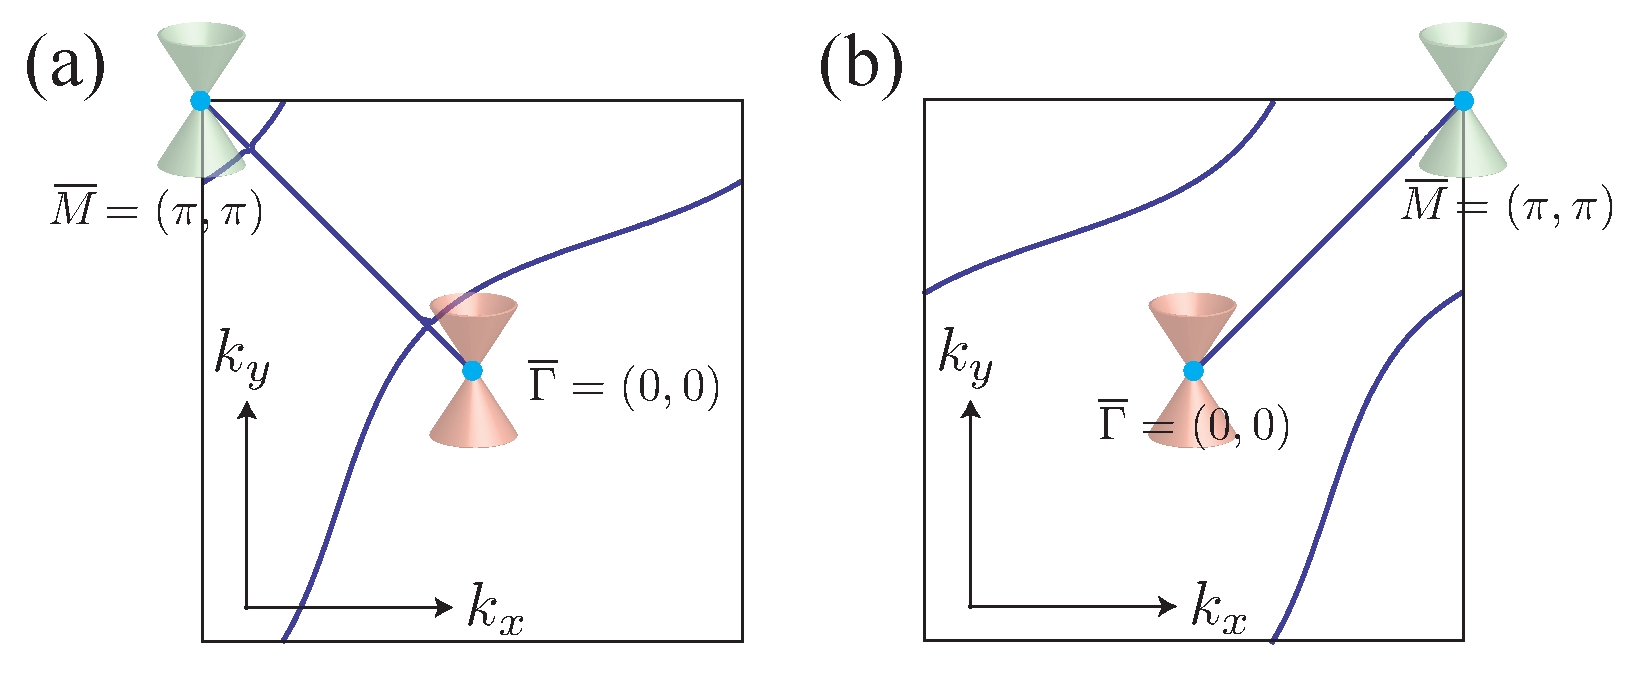
\includegraphics[width=0.8\textwidth]{fermiarc2}\caption[Fermi arcs on the $(001)$ surface with alternative boundary conditions]{Fermi arcs (blue lines) on the $(001)$ surface with alternative boundary conditions (a) $g(k_x,k_y)=-it_1$ and (b) $g(k_x,k_y)=-t_2e^{-ik_y}$ in the insulating domain, for $t_2/t_1=2$.}\label{fig:fermiarc2}\end{figure}

We notice that in the insulating phase (or on the boundary surface), Dirac wires can be backscattered with a different phase and dimerized out of the unit cell. These different boundary conditions correspond to distinct surface Fermi arc patterns. Figure~\ref{fig:fermiarc2} shows two alternatives. (a) shows the zero energy arcs when intra-cell backscattering reverses sign $t_1\to-t_1$ in the insulating domain. (b) shows a case when the dimerization is taken along the off-diagonal axis. These inequivalent boundary conditions differ by some three dimensional integer quantum Hall states, which correspond to additional chiral Fermi arcs that wrap non-trivial cycles around the 2D toric surface Brillouin zone.

\subsubsection{AFTR preserving surfaces}\label{sec:fermiarcAFTRpreserving}

We also notice that the Fermi arc structures in Figs.~\ref{fig:fermiarc1}(b) and \ref{fig:fermiarc2} are allowed because both the \AFTR symmetries $\mathcal{T}_{11}$, $\mathcal{T}_{\bar{1}1}$ and the $C_2$ symmetry are broken by the insulating domain. Any dimerization that preserves only one of $\mathcal{T}_{11}$ and $\mathcal{T}_{\bar{1}1}$ necessarily breaks translation symmetry, and corresponds to an enlarged unit cell and a reduced Brillouin zone (c.f.~Fig.~\ref{fig:Chernstack} and \ref{fig:DiracTB}). As a result, the two Weyl points would now collapse onto the same $\overline{\Gamma}$ point. Any momentum plane that contains the $k_z$-direction and avoids the $\Gamma$ point must have trivial Chern invariant, because it could always be deformed (while containing the $k_z$-direction and avoiding the $\Gamma$ point) to the reduced Brillouin zone boundary, where its Chern invariant would be killed by the \AFTR symmetry. %There would therefore be no protected surface Fermi arcs.

However, the trivial bulk Chern invariant does not imply the absence of surface state. This can be understood by looking at the surface boundary in real space. Here, we assume the Dirac strings that constitute the coupled wire model \eqref{WeylTBHam} are supported by vortices of an underlying Dirac mass (see Fig.~\ref{fig:vortexlattice} and eq.\eqref{DiracHam}). The semimetallic coupled wire model terminates along the $xy$-plane against vacuum, which is modeled by the Dirac insulator $H_{\mathrm{vacuum}}=\hbar v{\bf k}\cdot\vec{s}\mu_z+m_0\mu_x$, say with $m_0>0$. Recall from \eqref{massT11} that the Dirac mass vortex configuration \eqref{Jacobielliptic} is \AFTR symmetric along the $\mathcal{T}_{11}$-directions. The Dirac insulating vacuum is symmetric under local \TR as well as continuous translation. It however breaks the screw rotation symmetry $\hat{C}_2=is_z\mu_z$, but we here only focus on the \AFTR symmetry.

\begin{figure}[htbp]
	\centering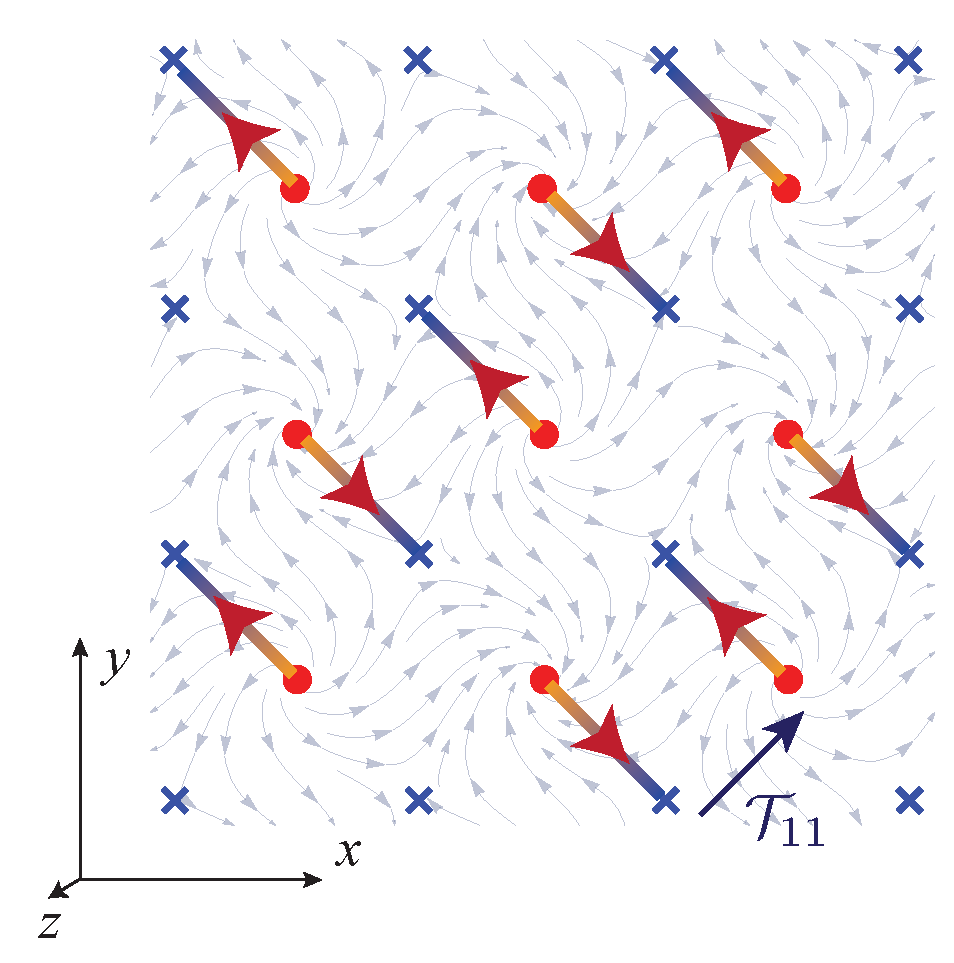
\includegraphics[width=0.6\textwidth]{SurfaceStates1bdy}
	\caption{Surface chiral Dirac channels of the coupled wire model \eqref{WeylTBHam} terminated along the $xy$ plane.}\label{fig:SurfaceStates1bdy}
\end{figure}

The surface boundary supports chiral Dirac channels that connect the chiral Dirac strings in the semimetallic bulk that are normal to the surface. The surface channels are shown in Fig.~\ref{fig:SurfaceStates1bdy}. The {\color{blue}$\times$} ({\color{red}$\bullet$}) represent chiral vortices in the bulk that direct electrons away from (resp.~onto) the surface. The vector field represents the Dirac mass $m({\bf r})=m_x({\bf r})+im_y({\bf r})$ modulation in the semimetallic bulk near the surface. The surface Dirac line channels~\cite{TeoKane} -- shown by directed lines connecting the bulk Dirac strings {\color{blue}$\times$}, {\color{red}$\bullet$} -- are located where the \TR symmetric Dirac mass $m_x$ changes sign across the surface boundary and the \TR breaking Dirac mass $m_y$ flips sign across the line channels along the surface. In other words, they are traced out of points on the surface where $m_x<0$ and $m_y=0$. Each of these surface channels carries a chiral Dirac electronic mode that connects the bulk chiral Dirac vortices. They can couple through inter-channel electron tunneling, but the collective gapless surface state cannot be removed from low-energy by dimerization without breaking the \AFTR symmetry $\mathcal{T}_{11}$. %The surface state is, in a sense, half of that of a weak topological insulator (or 3D stack of quantum spin Hall layers). 


\section{Many-body interacting variations}\label{sec:intenable}

We discuss the effect of strong many-body interactions in a Dirac semimetal in three dimensions. Before we do so, it is worth stepping back and reviewing the two dimensional case in order to illustrate the issue and idea that will be considered and generalized in three dimensions. The massless Dirac fermion with $H=\hbar v(k_xs_y-k_ys_x)$ that appears on the surface of a topological insulator~\cite{HasanKane10,QiZhangreview11,HasanMoore11,RMP} is protected by time reversal (TR) and charge $U(1)$ symmetries and is anomalous. This means that there is no single-body energy gap opening mass term that preserves the symmetries, and there is no single-body fermionic lattice model in two dimensions that supports a massless Dirac fermion without breaking the symmetries. Neither of these statements hold true in the many-body setting. The surface Dirac fermion can acquire a \TR and charge $U(1)$ preserving many-body interacting mass.~\cite{WangPotterSenthilgapTI13,ChenFidkowskiVishwanath14,MetlitskiKaneFisher13b,BondersonNayakQi13} Consequently, this also enables a massless symmetry preserving Dirac fermion in a pure 2D system without holographically relying on a semi-infinite 3D topological bulk. For instance, one can take a quasi-2D topological insulator slab with finite thickness and remove the Dirac fermion on one of the two surfaces by introducing an interacting mass gap. This leaves a single massless Dirac fermion on the opposite surface without breaking symmetries.

A massless Dirac fermion in three dimensional semimetallic materials can be protected in the single-body picture by screw rotation, time reversal and charge $U(1)$ symmetries (see reviews Ref.~\cite{Ashvin_Weyl_review,RMP,ArmitageMeleVishwanath16} and Sec.~\ref{sec:DiracSemimetal}). From a theory point of view, it can be supported on the 3D boundary of a 4D weak topological insulator, where the two Weyl fermions are located at distinct time reversal invariant momenta (recall Fig.~\ref{fig:Weylspectrum} and Sec.~\ref{sec:holproj4D} for the antiferromagnetic case). In this case, the massless fermions are protected by translation, time reversal and charge $U(1)$ symmetries. In this section, we address the following issues. (1) We show by explicitly constructing an exactly solvable coupled wire model that the 3D Dirac fermion can acquire a many-body interacting mass while preserving all symmetries. (2) We show in principle that an antiferromagnetic time reversal (AFTR) symmetric massless 3D Dirac system with two Weyl fermions separated in momentum space can be enabled by many-body interactions without holographically relying on a higher dimensional topological bulk.

We begin with the Dirac semimetallic coupled wire model in Fig.~\ref{fig:Weylspectrum} and \eqref{WeylTBHam}. In particular, we focus on many-body interactions that facilitate the fractionalization of a $(1+1)$D chiral Dirac channel \begin{align}\mathrm{Dirac}=\mathrm{Pfaffian}\otimes\mathrm{Pfaffian}\label{fractionalization}\end{align} (see also Fig.~\ref{fig:glueingsplitting}). In a sense, each chiral Pfaffian channel carries half of the degrees of freedom of the Dirac. For instance, it has half the electric and thermal conductances, which are characterized by the filling fraction $\nu=1/2$ and the chiral central charge $c=1/2$ in \eqref{conductance}. Throughout this dissertation, we refer to the low-energy effective \CFT -- that consists of an electrically charged $U(1)_4$ bosonic component, say moving in the $R$ direction, and a neutral Majorana fermion component moving in the opposite $L$ direction -- simply as a Pfaffian \CFT \begin{align}\mathrm{Pfaffian}=U(1)_4\otimes\overline{\mathrm{Ising}}.\label{PfaffianCFT}\end{align} (In this article, we follow the level convention for $U(1)$ in the \CFT community~\cite{bigyellowbook}. The same theory may be more commonly referred to as $U(1)_8$ in the fractional quantum Hall community. For clarification, see Lagrangian \eqref{Pfaffian} and \eqref{LFQHCS}.)

While this is not the focus of this article, here we clarify and disambiguate the three ``Pfaffian" fractional quantum Hall (\hypertarget{FQH}{FQH}) states that commonly appear in the literature. All these $(2+1)$D states are theorized at filling fraction $\nu=1/2$, although being applied to $\nu=5/2$ in materials, and have identical electric transport properties. However, they have distinct thermal Hall transport behaviors. They all have very similar anyonic quasiparticle (\hypertarget{QP}{QP}) structures. For instance, they all have four Abelian and two non-Abelian \QP (up to the electron). On the other hand, the charge $e/4$ non-Abelian Ising anyons of the three states have different spin-exchange statistics. First, the gapless boundary of the Moore-Read Pfaffian \FQH state~\cite{MooreRead,ReadMoore,GreiterWenWilczekPRL91,GreiterWenWilczek91} can be described by the $(1+1)$D chiral \CFT $U(1)_4\otimes\mathrm{Ising}$ where the charged boson and neutral fermion sectors are co-propagating. It therefore carries the chiral central charge $c=1+1/2=3/2$, which dictates the thermal Hall response \eqref{conductance}. Second, the ``anti-Pfaffian" \FQH state~\cite{LevinHalperinRosenow07,LeeRyuNayakFisher07} is the particle-hole conjugate of the Moore-Read Pfaffian state. Instead of half-filling the lowest Landau level by electrons, one can begin with the completely filled lowest Landau level, and half-fill it with holes. In a sense the anti-Pfaffian state is obtained by subtracting the completely filled lowest Landau level by a Moore-Read Pfaffian state. Along the boundary, the $(1+1)$D \CFT $U(1)_{1/2}\otimes\overline{U(1)_4\otimes\mathrm{Ising}}$ consists of the forward propagating chiral Dirac $U(1)_{1/2}$ sector that corresponds to the lowest Landau level, and the backward propagating Moore-Read Pfaffian $\overline{U(1)_4\otimes\mathrm{Ising}}$. Here $\overline{\mathcal{C}}$ can be interpreted as the time-reversal conjugate of the chiral \CFT $\mathcal{C}$. The thermal transport is governed by the edge chiral central charge $c=1-3/2=-1/2$, which has an opposite sign from the filling fraction. Thus, unlike the Moore-Read Pfaffian state, the net electric and thermal currents now travel in opposite directions along the edge. Lastly, the recently proposed particle-hole symmetric (\hypertarget{PHS}{PHS}) Pfaffian state~\cite{Son15,BarkeshliMulliganFisher15,WangSenthil16}, which is going to be the {\em only} Pfaffian \FQH state considered in this article (see Ref.~\cite{KaneSternHalperin17} for a coupled wire construction), has the chiral edge \CFT \eqref{PfaffianCFT}. As the electrically charged boson and neutral fermion sectors are counter-propagating, the net thermal edge transport is governed by the chiral central charge $c=1-1/2=1/2$. The chiral $(1+1)$D \PHS Pfaffian \CFT \eqref{PfaffianCFT} is also present along the line interface separating a \TR symmetric $\mathcal{T}$-Pfaffian~\cite{ChenFidkowskiVishwanath14} domain and a \TR breaking magnetic domain on the surface of a 3D topological insulator. (Similar constructions can be applied to alternative \TR symmetric topological insulator surface states~\cite{WangPotterSenthilgapTI13,MetlitskiKaneFisher13b,BondersonNayakQi13}, but they will not be considered in this article.) Other than their thermal transport properties, the three Pfaffian \FQH state can also be distinguished by the charge $e/4$ Ising anyon, which has spin $h=1/8$, $-1/8$ or $0$ for the Moore-Read Pfaffian, anti-Pfaffian or \PHS Pfaffian states respectively. 

Since we will not be considering the Moore-Read Pfaffian or its particle-hole conjugate anti-Pfaffian state, we will simply refer to the \PHS Pfaffian state as the Pfaffian state. The low-energy effective chiral $(1+1)$D \CFT takes the decoupled form between the boson and fermion \begin{align}\mathcal{L}_{\mathrm{Pfaffian}}&=\mathcal{L}_{\mathrm{charged}}+\mathcal{L}_{\mathrm{neutral}} \,, \label{Pfaffian}\\&=\frac{8}{2\pi}\partial_t\phi_R\partial_x\phi_R+v(\partial_x\phi_R)^2\nonumber\\&\;\;\;+i\gamma_L(\partial_t-\tilde{v}\partial_x)\gamma_L\nonumber \,, \end{align} where we have set $\hbar=1$. Here $\phi_R$ is the free chiral $U(1)_4$ boson. It generates the $(1+1)$D theory $\mathcal{L}_{\mathrm{charged}}$, which is identical to the boundary edge theory of the $(2+1)$D bosonic Laughlin $\nu=1/8$ fractional quantum Hall state described by the topological Chern-Simon theory~\cite{WenZee92,Wenedgereview} \begin{align}\mathcal{L}_{2+1}=\frac{K}{4\pi}\alpha\wedge d\alpha+et\alpha\wedge dA \,, \label{LFQHCS}\end{align} with $K=8$ and $t=2$. The $U(1)_4$ \CFT carries the electric conductance $\sigma=tK^{-1}t=1/2$ in units of $2\pi e^2=e^2/h$ and a thermal conductance characterized by the chiral central charge $c=c_R=1$. Primary fields are of the form of (normal ordered) chiral vertex operators $:e^{im\phi_R}:$, for $m$ an integer, and carries charge $q=m/4$ in units of $e$ and conformal scaling dimension (i.e.~conformal spin) $h=h_R=m^2/16$. We summarize and abbreviate the operator product expansion \begin{align}e^{im_1\phi_R(z)}e^{im_2\phi_R(w)}=e^{i(m_1+m_2)\phi_R(w)}(z-w)^{m_1m_2/8}+\ldots\end{align} by the Abelian fusion rule \begin{align}e^{im_1\phi_R}\times e^{im_2\phi_R}=e^{i(m_1+m_2)\phi_R},\end{align} where $z\sim\tau+ix$ is the complex space-time parameter and $\tau=i\pi vt/2$ is the Euclidean time.

$\gamma_L^\dagger=\gamma_L$ is the free Majorana fermion. It generates the $(1+1)$D theory $\mathcal{L}_{\mathrm{neutral}}$, which is equivalent to a chiral component of the critical Ising \CFT or the boundary edge theory of the $(2+1)$D Kitaev honeycomb model~\cite{Kitaev06} in its B-phase with \TR breaking (i.e.~a chiral $p_x+ip_y$ superconductor coupled with a $\mathbb{Z}_2$ gauge theory). It carries trivial electric conductance but contributes to a finite thermal conductance characterized by the chiral central charge $c=-c_L=-1/2$. The Ising \CFT has primary fields $1$, $\gamma_L$ and $\sigma_L$, where the twist field (or Ising anyon) $\sigma_L$ carries the conformal spin $h=-h_L=-1/16$. Again, we abbreviate the operator product expansions \begin{gather}\gamma_L(\bar{z})\gamma_L(\bar{w})=\frac{1}{\bar{z}-\bar{w}}+\ldots\nonumber \,, \\\sigma_L(\bar{z})\gamma_L(\bar{w})=\frac{\sigma_L(\bar{w})}{(\bar{z}-\bar{w})^{1/2}}+\ldots\nonumber \,, \\\sigma_L(\bar{z})\sigma_L(\bar{w})=\frac{1}{(\bar{z}-\bar{w})^{1/8}}+(\bar{z}-\bar{w})^{3/8}\gamma_L(\bar{w})\nonumber \end{gather} by the fusion rule \begin{gather}\gamma_L\times\gamma_L=1,\quad\sigma_L\times\gamma_L=\sigma_L\nonumber \,, \\\sigma_L\times\sigma_L=1+\gamma_L,\end{gather} where $\bar{z}\sim\tau-ix$ is the complex space-time parameter and $\tau=i\tilde{v}t$ is the Euclidean time. 

General primary fields of the Pfaffian \CFT decompose into the $U(1)_4$ part and the Ising part. They take the form \begin{align}1_m=e^{im\phi_R},\quad\psi_m=e^{im\phi_R}\gamma_L,\quad\sigma_m=e^{im\phi_R}\sigma_L.\label{Pfaffianfields}\end{align} The conformal spins and fusion rules also decompose so that \begin{align}h_{1_m}=\frac{m^2}{16},\quad h_{\psi_m}=\frac{m^2}{16}+\frac{1}{2},\quad h_{\sigma_m}=\frac{m^2-1}{16}\end{align} modulo 1, $q_m=m/4$ in units of $e$, and \begin{gather}1_{m_1}\times1_{m_2}=\psi_{m_1}\times\psi_{m_2}=1_{m_1+m_2}\nonumber \,, \\1_{m_1}\times\psi_{m_2}=\psi_{m_1+m_2}\nonumber \,, \\1_{m_1}\times\sigma_{m_2}=\psi_{m_1}\times\sigma_{m_2}=\sigma_{m_1+m_2}\nonumber \,, \\\sigma_{m_1}\times\sigma_{m_2}=1_{m_1+m_2}+\psi_{m_1+m_2}.\end{gather} The $2\pi$ monodromy phase $\mathcal{M}^{XY}_Z=R^{XY}_ZR^{YX}_Z$ between primary fields $X$ and $Y$ with a fixed overall fusion channel $Z$ can be deduced by the {\em ribbon identity}~\cite{Kitaev06} \begin{align}e^{2\pi ih_Z}=\vcenter{\hbox{
\includegraphics[width=0.5in]{ribbon1.pdf}}}=\vcenter{\hbox{
\includegraphics[width=0.5in]{ribbon2.pdf}}}=\mathcal{M}^{XY}_Ze^{2\pi i(h_X+h_Y)}\label{ribbonapp}\end{align} for $h_{X,Y,Z}$ the conformal spins for primary fields $X,Y,Z$. Unlike the gauge dependent $\pi$-exchange phase $R^{XY}_Z$, the $2\pi$-monodromy phase $\mathcal{M}^{XY}_Z=e^{2\pi i(h_Z-h_X-h_Y)}$ is gauge independent and physical.

The electronic quasiparticle is the composition $\psi_{\mathrm{el}}=e^{-i4\phi_R}\gamma_L$ so that it is fermionic and has electric charge $-1$ in units of $e$. Since electron is the fundamental building block of the system, locality of $\psi_{\mathrm{el}}$ only allows primary fields $X$ that have trivial monodromy $\mathcal{M}^{X,\psi_{\mathrm{el}}}=1$ with the electron. As a result, this restricts $1_m,\psi_m$ to even $m$ and $\sigma_m$ to odd $m$. Lastly, the coupled wire models constructed later will involve the Pfaffian channels that propagate in both forward and backward directions. We will denote the backward case by $\overline{\mathrm{Pfaffian}}$, whose Lagrangian density is the time reversal of \eqref{Pfaffian}, i.e.~replacing $R\leftrightarrow L$, $i\leftrightarrow-i$ and $\partial_t\leftrightarrow-\partial_t$. 

\subsection{Gluing and splitting}\label{sec:gluing}

\begin{figure}[htbp]
	\centering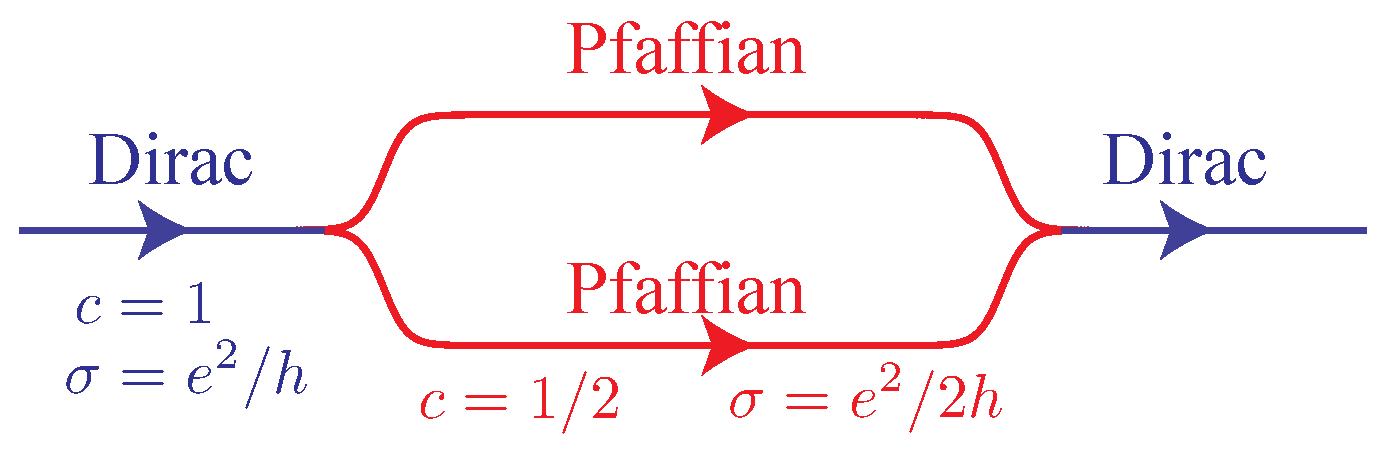
\includegraphics[width=0.6\textwidth]{glueingsplitting}
	\caption{Gluing and splitting a pair of chiral Pfaffian 1D channels into and from a chiral Dirac channel.}\label{fig:glueingsplitting}
\end{figure}

A pair of co-propagating Pfaffian \CFT can be ``glued" together into a single chiral Dirac electronic channel. We first consider the decoupled pair $\mathcal{L}_0=\mathcal{L}_{\mathrm{Pfaffian}}^A+\mathcal{L}_{\mathrm{Pfaffian}}^B$, where $\mathcal{L}_{\mathrm{Pfaffian}}^{A/B}$ is the Lagrangian density of one of the two Pfaffian \CFT labeled by $A,B$. The pair of Majorana fermions can compose an electrically neutral Dirac fermion $d_L=(\gamma^A_L+i\gamma^B_L)/\sqrt{2}$, which can then be bosonized $d_L\sim e^{i\phi^\sigma_L}$, for $\phi^\sigma_L$ the chiral $\overline{U(1)_{1/2}}$ boson. The bare Lagrangian now becomes the multi-component $U(1)_4^A\otimes U(1)_4^B\otimes\overline{U(1)_{1/2}}$ boson \CFT \begin{align}\mathcal{L}_0=\frac{1}{2\pi}\partial_t\boldsymbol{\phi}^TK\partial_x\boldsymbol{\phi}+\partial_x\boldsymbol{\phi}^TV\partial_x\boldsymbol{\phi},\label{881}\end{align} where $\boldsymbol{\phi}=(\phi_R^A,\phi_R^B,\phi^\sigma_L)$, $K$ is the $3\times3$ diagonal matrix $K=\mathrm{diag}(8,8,-1)$, and $V$ is some non-universal velocity matrix. A primary field is a vertex operator $e^{i{\bf m}\cdot\boldsymbol{\phi}}$ labeled by an integral vector ${\bf m}=(m^A,m^B,\tilde{m})$. It carries conformal spin $h_{\bf m}={\bf m}^TK^{-1}{\bf m}/2$ and electric charge $q_{\bf m}={\bf t}^TK^{-1}{\bf m}$ in units of $e$, where ${\bf t}=(2,2,0)$ is the charge vector. As ${\bf n}=(1,-1,4)$ is an electrically neutral null vector (i.e.~${\bf n}^TK{\bf n}=0$ and ${\bf t}\cdot{\bf n}=0$), it corresponds to the charge $U(1)$ preserving backscattering coupling \begin{align}\delta\mathcal{H}=-u\cos\left({\bf n}^TK\boldsymbol{\phi}\right)=-u\cos\left(8\phi^A_R-8\phi^B_R-4\phi^\sigma_L\right)\label{glueingH}\end{align} that gaps~\cite{Haldane95} and annihilates a pair of counter-propagating boson modes. The interacting Hamiltonian can also be expressed in terms of many-body backscattering of the Pfaffians' primary fields \begin{align}\delta\mathcal{H}=-u:\left(d_L^\dagger d_R\right)^4:+h.c. \,,\end{align} where $d_R=1_2^A1_{-2}^B$ is the electrically neutral Dirac fermion composed of the pair of oppositely charged semions in the two Pfaffian sectors.

In strong coupling, the gapping Hamiltonian introduces an interacting mass and the ground state expectation value $\langle\Phi\rangle=n\pi/2$, for $n$ an integer and $\Phi=2\phi^A_R-2\phi^B_R-\phi^\sigma_L$. In low energy, it leaves behind the chiral boson combination $\tilde\phi_R=2\phi_R^A+2\phi_R^B$, which has trivial operator product (i.e.~commutes at equal time) with the order parameter $\Phi$. The low-energy theory after projecting out the gapped sectors becomes \begin{align}\mathcal{L}_0-\delta\mathcal{H}\longrightarrow\mathcal{L}_{\mathrm{Dirac}}=\frac{1}{2\pi}\partial_t\tilde\phi_R\partial_x\tilde\phi_R+v(\partial_x\tilde\phi_R)^2 \,, \end{align} which is identical to the bosonized Lagrangian density of a chiral Dirac fermion. For instance, the vertex operator $\psi_R^{\mathrm{el}}\sim e^{i\tilde\phi_R}\sim 1_2^A1_2^B$ has the appropriate spin and electric charge of an electronic Dirac fermion operator ($h=1/2$ and $q=1$ in units of $e$). Notice that the vertex operator $e^{i\tilde\phi_R/2}$ has $-1$ monodromy with the local electronic $\psi_R^{\mathrm{el}}$ and therefore is not an allowed excitation in the fermionic theory.

We notice in passing that the gluing potential \eqref{glueingH} facilitates an anyon condensation process~\cite{BaisSlingerlandCondensation}, where the maximal set of mutually local neutral bosonic anyon pairs \begin{align}\begin{array}{*{20}c}1_{4m}^A1_{-4m}^B,\psi_{4m}^A\psi_{-4m}^B,\\\psi_{4m+2}^A1_{-4m-2}^B,1_{4m+2}^A\psi_{-4m-2}^B,\sigma_{4m+1}^A\sigma_{-4m-1}^B\end{array}\label{condensebosons}\end{align} is condensed, where $m$ is an arbitrary integer. All primary fields that are non-local (i.e.~with non-trivial monodromy) with any of the condensed bosons in \eqref{condensebosons} are confined. Any two primary fields that differ from each other by a condensed boson in \eqref{condensebosons} are now equivalent. The condensation therefore leaves behind the electronic Dirac fermion \begin{align}\psi^{\mathrm{el}}_R=\psi^A_4\equiv\psi^B_4\equiv1_2^A1_2^B\end{align} and its combinations. 

\begin{figure}[htbp]
	\centering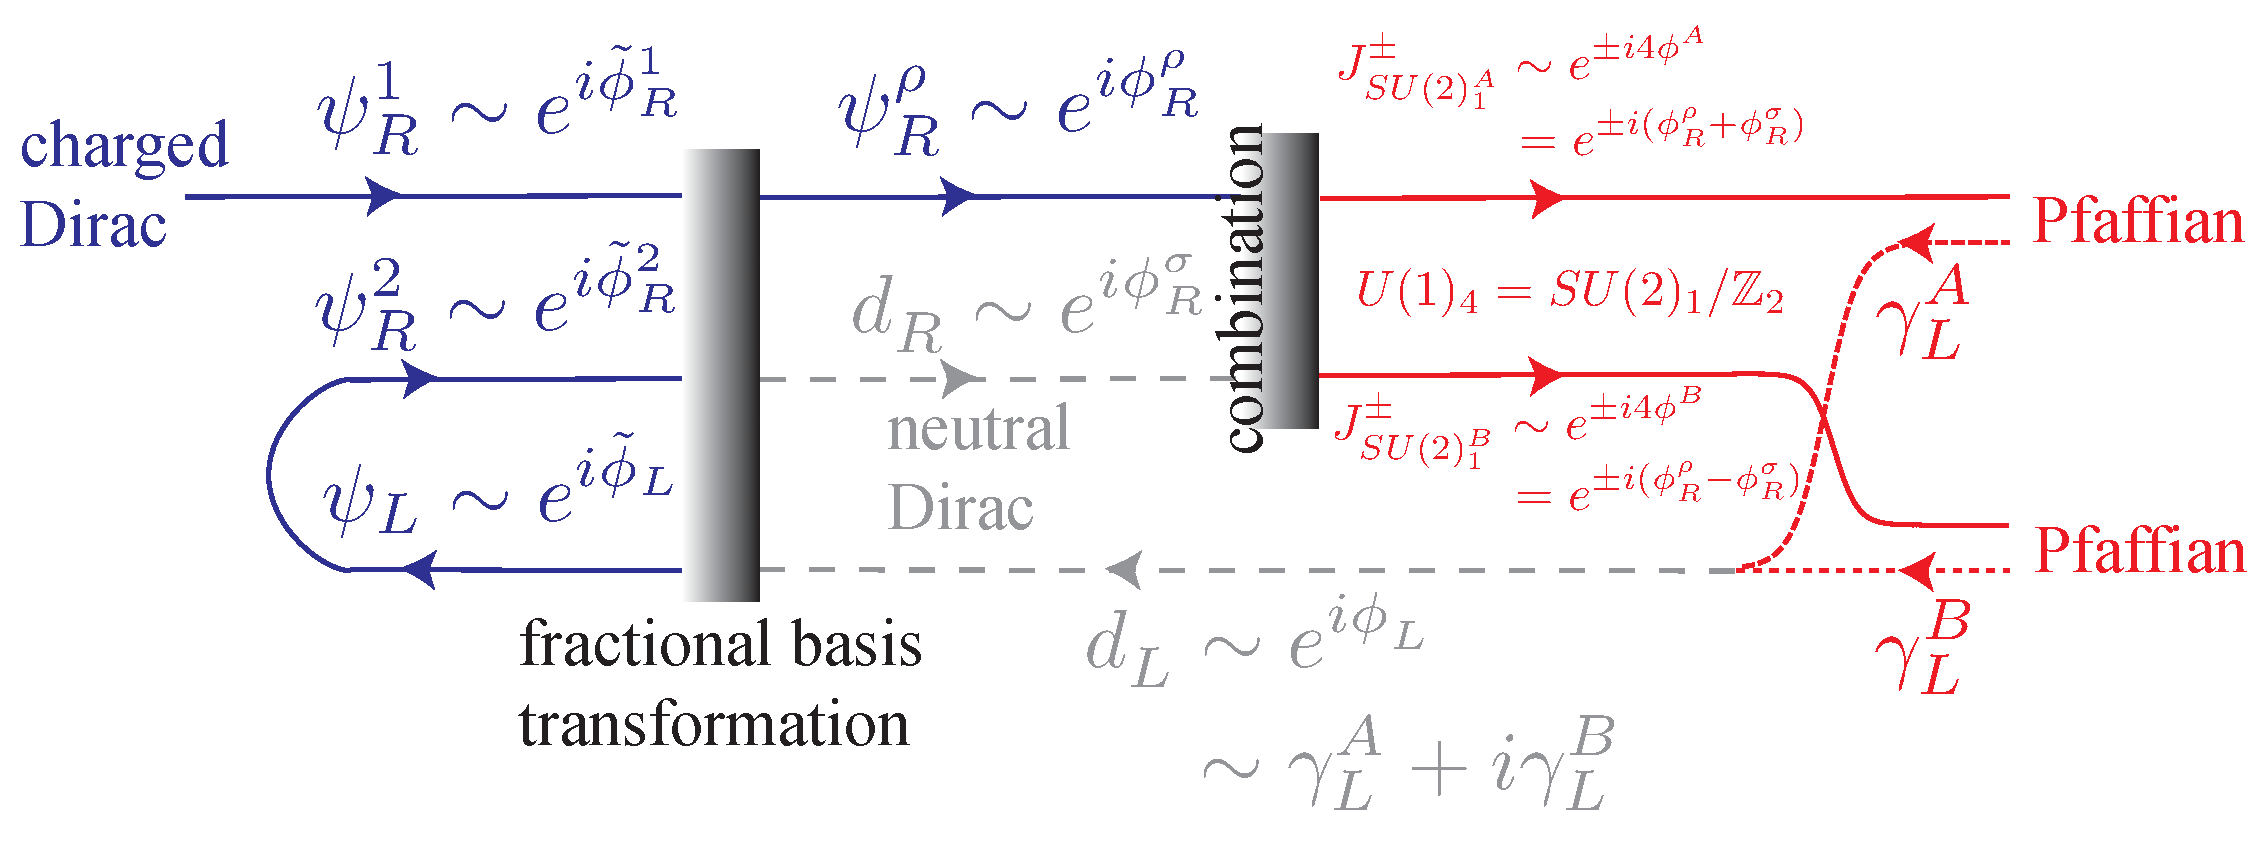
\includegraphics[width=1\textwidth]{fractionalization}
	\caption{Schematics of splitting a chiral Dirac channel into a pair of Pfaffian channels.}\label{fig:fractionalization}
\end{figure}

On the other hand, a chiral Dirac channel can be decomposed into a pair of chiral Pfaffian channels (see Fig.~\ref{fig:fractionalization} for a summary). First, perhaps from some channel re-construction, we append to the chiral Dirac channel an additional pair of counter-propagating Dirac modes. This can be realized by pulling a parabolic electronic/hole band from the conduction/valence band to the Fermi level, or introducing non-linear dispersion to the original chiral channel. In low-energy, the three Dirac fermion modes can be bosonized $\psi^{1,2}_R\sim e^{i\tilde\phi_R^{1,2}}$, $\psi_L\sim e^{-i\tilde\phi_L}$ and they are described by the multicomponent boson Lagrangian \begin{align}\widetilde{\mathcal{L}}_{\mathrm{Dirac}}=\frac{1}{2\pi}\partial_t\widetilde{\boldsymbol\phi}^T\tilde{K}\partial_x\widetilde{\boldsymbol\phi}+\partial_x\widetilde{\boldsymbol\phi}^T\tilde{V}\partial_x\widetilde{\boldsymbol\phi}\label{3Dirac}\end{align} for $\widetilde{\boldsymbol\phi}=(\tilde\phi_R^1,\tilde\phi_R^2,\tilde\phi_L)$, $\tilde{K}$ is the diagonal matrix $\tilde{K}=\mathrm{diag}(1,1,-1)$, and $\tilde{V}$ is some non-universal velocity matrix. A general composite excitation can be expressed by a vertex operator $e^{i{\bf m}\cdot\widetilde{\boldsymbol\phi}}$, for ${\bf m}$ an integral 3-vector, with spin $h_{\bf m}=|{\bf m}|^2/2$ and electric charge $q_{\bf m}={\bf m}^T\tilde{K}\tilde{\bf t}$ in units of $e$, where $\tilde{\bf t}=(1,1,1)$ is the charge vector.

Next we perform a {\em fractional} basis transformation \begin{align}\begin{array}{*{20}l}\phi^\rho_R=\tilde\phi^1_R+\tilde\phi^2_R+\tilde\phi_L \,, \\\phi^\sigma_R=\tilde\phi^1_R-\frac{1}{2}\tilde\phi^2_R+\frac{1}{2}\tilde\phi_L \,,\\\phi^\sigma_L=\tilde\phi^1_R+\frac{1}{2}\tilde\phi^2_R+\frac{3}{2}\tilde\phi_L \,.\end{array}\label{fracbasistrans0}\end{align} While the $\tilde{K}$ matrix is invariant under the transformation, the charge vector changes to $\tilde{\bf t}\to(1,0,0)$. $\psi^\rho_R\sim e^{i\phi^\rho_R}$ is the local electronic Dirac fermion that carries spin $1/2$ and electric charge $e$, and $d_{R/L}\sim e^{i\phi^\sigma_{R/L}}$ are counter-propagating electrically neutral Dirac fermions. As the $\tilde{K}$ matrix is still diagonal, these fermions have trivial mutual $2\pi$-monodromy and are local with respect to each other. However, it is important to notice that the neutral Dirac fermions $d_{R/L}$ actually consist of fractional electronic components.

Now we focus on the two $R$-moving Dirac channels. By pairing the Dirac fermions, they form two independent $SU(2)_1$ Kac-Moody current operators~\cite{bigyellowbook} \begin{align}J_3^{A/B}(z)&=i2\sqrt{2}\partial_z\phi^{A/B}_R(z)\label{SU2current} \,, \\J_\pm^{A/B}(z)&=\frac{J_1^{A/B}(z)\pm iJ_2^{A/B}(z)}{\sqrt{2}}=e^{\pm i4\phi^{A/B}_R(z)}\nonumber \,, \end{align} where $4\phi^A_R=\phi^\rho_R+\phi^\sigma_R$ and $4\phi^B_R=\phi^\rho_R-\phi^\sigma_R$. Both $SU(2)_1$ sectors are electrically charged so that the bosonic vertex operators $J_\pm^{A/B}$ carries charge $\pm e$. They obey the $SU(2)$ current algebra at level 1 \begin{align}J^\lambda_{\mathsf{i}}(z)J^{\lambda'}_{\mathsf{j}}(w)=\frac{\delta^{\lambda\lambda'}\delta_{\mathsf{ij}}}{(z-w)^2}+\sum_{\mathsf{k}=1}^3\frac{i\sqrt{2}\delta^{\lambda\lambda'}\varepsilon_{\mathsf{ijk}}}{z-w}J^\lambda_{\mathsf{k}}(w)+\ldots\label{SU2algebra}\end{align} for $\lambda,\lambda'=A,B$. It is crucial to remember that $J_\pm^A\sim\psi^\rho_Rd_R$ and $J_\pm^B\sim\psi^\rho_Rd_R^\dagger$ contains the fractional Dirac components $d_R$. Thus, the primitive local bosons are actually pairs of the current operators, i.e.~$e^{i8\phi^{A/B}_R}$. Equivalently, this renormalizes the compactification radius of the boson $4\phi^{A/B}_R$ so that in a closed periodic space-time geometry, we only require electronic Cooper pair combinations such as the charge $2e$ local operators \begin{gather}e^{i8\phi^A_R}=e^{i(4\tilde\phi^1_R+\tilde\phi^2_R+3\tilde\phi_L)}\sim(\psi^1_R)^4\psi^2_R(\psi_L^\dagger)^3\nonumber \,, \\e^{i8\phi^B_R}=e^{i(3\tilde\phi^2_R+\tilde\phi_L)}\sim(\psi^2_R)^3\psi_L^\dagger\end{gather} to be periodic. The incorporation of anti-periodic boundary condition for $J_\pm^{A/B}=e^{\pm i4\phi^{A/B}_R}$ results in the $\mathbb{Z}_2$-orbifold theory~\cite{Ginsparg88,DijkgraafVafaVerlindeVerlinde99} $U(1)_4=SU(2)_1/\mathbb{Z}_2$ for both $A$ and $B$ sectors. For instance, the primitive twist fields are given by $e^{\pm i\phi^{A/B}_R}$, which have $-1$ monodromy phase with $J_\pm^{A/B}$. 

At this point, including the $L$-moving neutral Dirac sector, we have recovered the muticomponent boson $\boldsymbol\phi=(\phi^A_R,\phi^B_R,\phi^\sigma_L)$ described by the Lagrangian \eqref{881}. Lastly, we simply have to decompose the remaining neutral Dirac into Majorana components, $d_L=(\gamma^A_L+i\gamma^B_L)/\sqrt{2}$. The $A$ and $B$ Pfaffian sectors can then be independently generated by the charged $U(1)_4$ boson $\phi^{A/B}_R$ and the neutral Majorana fermion $\gamma^{A/B}_L$. As a consistency check, the charge $e$ fermionic (normal ordered) combinations defined in \eqref{Pfaffianfields} \begin{align}\psi_4^A&\sim e^{i4\phi^A_R}\gamma_L^A\sim e^{i\tilde\phi^1_R}+e^{i(3\tilde\phi^1_R+\tilde\phi^2_R+3\tilde\phi_L)}\label{psi4def1} \,, \\\psi_4^B&\sim e^{i4\phi^B_R}\gamma_L^B\sim e^{i(-\tilde\phi^1_R+\tilde\phi^2_R-\tilde\phi_L)}-e^{i(\tilde\phi^1_R+2\tilde\phi^2_R+2\tilde\phi_L)}\nonumber\end{align} are in fact local quasi-electronic. %(The minus sign in the bosonized expression for $\psi_4^A$ comes from the Klein factors defined later in \eqref{ETcomm0} and \eqref{ETcomm1}).

Unlike in the gluing case where there is a gapping Hamiltonian \eqref{glueingH} that pastes a pair of Pfaffians into a Dirac, here in the splitting case we have simply performed some kind of fractional basis transformation that allows us to express Dirac as a pair of Pfaffians. In fact, one can check that the energy-momentum tensor of the Dirac theory \eqref{3Dirac} is identical to that of a pair of Pfaffians \eqref{Pfaffian}. However, this does not mean the Pfaffian primary fields are natural stable excitations. In fact, as long as there is a pair of co-propagating Pfaffian channels, all primary fields except the non-fractionalized electronic ones are unstable against the gluing Hamiltonian $\delta\mathcal{H}$ in \eqref{glueingH} and are generically gapped. In order for the Pfaffian \CFT to be stabilized, one has to suppress $\delta\mathcal{H}$. A possible way is to somehow spatially separate the pair. This issue is addressed in the subsection below using many-body interaction in the coupled wire model of a Dirac semimetal (or the \PHS Pfaffian \FQH state in Ref.~\cite{KaneSternHalperin17}).

%\subsubsection{\texorpdfstring{$AB$}{AB} symmetry}
%The bi-partition $\mathrm{Dirac}=\mathrm{Pfaffian}^A\otimes\mathrm{Pfaffian}^B$ carries a flip symmetry that exchanges the two Pfaffian sectors. When the two Pfaffian channels are spatially separated (see Fig.~\ref{fig:glueingsplitting}), the flip symmetry is simply the twofold rotation that exchanges the two parallel channels along their center-of-mass axis. We will use this flip operation to generate the $C_2$ symmetry in the interacting coupled wire model in the next subsection. Focusing on a single wire, the twofold symmetry flips \begin{align}C_2\phi^{A/B}_RC_2^{-1}=\phi^{B/A}_R+\frac{\pi}{8},\quad C_2\phi^\sigma_LC_2^{-1}=\phi^\sigma_L+\frac{\pi}{2}.\end{align} The constants phases ensures the $2\pi$ rotation $C_2^2$ associates the appropriate $-1$ twist phase 
%$e^{2\pi ih_X}$ determined by the spin $h_X$ of the primary field $X$. 


\subsection{Symmetry preserving massive interacting model}\label{sec:interactionmodels}

We begin with the 3D array of chiral Dirac strings in Fig.~\ref{fig:vortexlattice}. In Sec.~\ref{sec:DiracSemimetal}, we showed that the single-body coupled wire model \eqref{WeylTBHam} described a Dirac semimetal with two Weyl fermions (see Fig.~\ref{fig:Weylspectrum}). The system had emergent antiferromagnetic time reversal (AFTR) symmetries $\mathcal{T}_{11}$ and $\mathcal{T}_{\bar{1}1}$ along the diagonal and off-diagonal axes (see \eqref{WeylTBT11}). Together they generate an emergent lattice translation symmetry with a 2-wire unit cell, and separate the two Weyl points in the Brillouin zone. The symmetries are lowered beyond the effective model when the microscopic high-energy degrees of freedom are included. For example, the mass function \eqref{Jacobielliptic} that supports the Dirac vortex string lattice has a 4-wire periodic unit cell and only preserves one of the \AFTR symmetries $\mathcal{T}_{11}$ (see \eqref{massT11}). With the lowered translation symmetry, the two Weyl points now coincide at the same momentum. Inter-species (or inter-valley) mixing is forbidden by the remaining \AFTR symmetry and a (screw) twofold rotation symmetry $C_2$ about $z$ (see \eqref{WeylTBC2} and \eqref{massC2}). Previously in Sec.~\ref{sec:brokensymmetry}, we introduced symmetry breaking wire dimerizations in \eqref{DiracTBHam} that led to a massive Dirac insulator. In this section, we construct many-body gapping interactions that preserves the two \AFTR symmetries $\mathcal{T}_{11}$ and $\mathcal{T}_{\bar{1}1}$, the $C_2$ symmetry, as well as charge $U(1)$ conservation. 

\begin{figure}[htbp]
	\centering
	(a)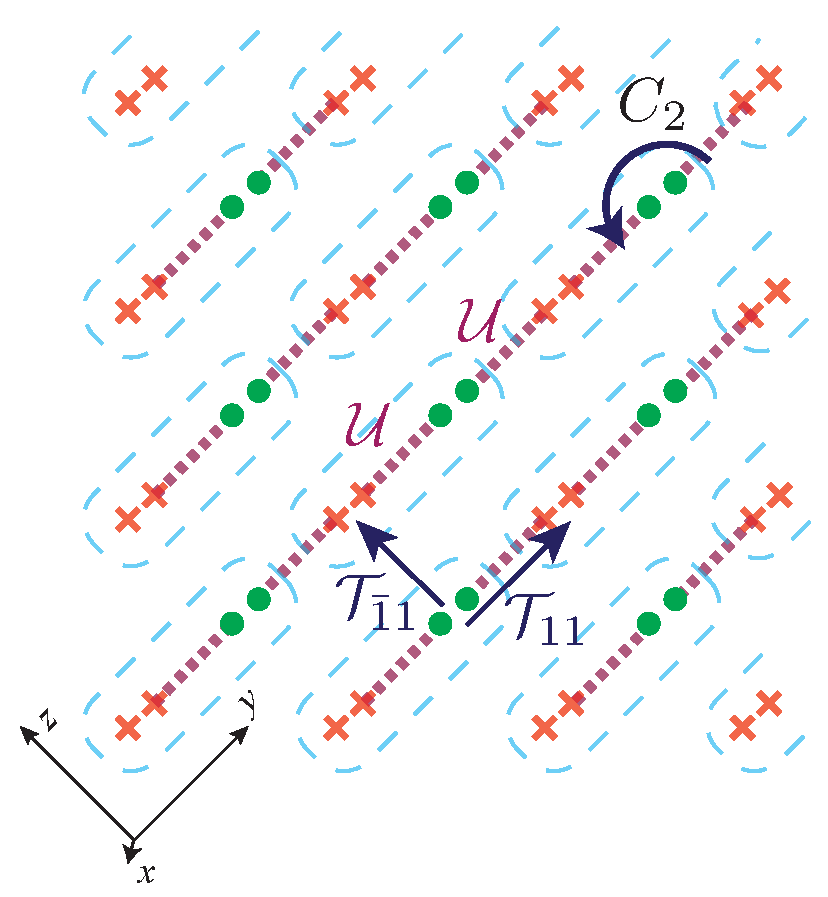
\includegraphics[width=0.5\textwidth]{gappinginteraction1}
	(b)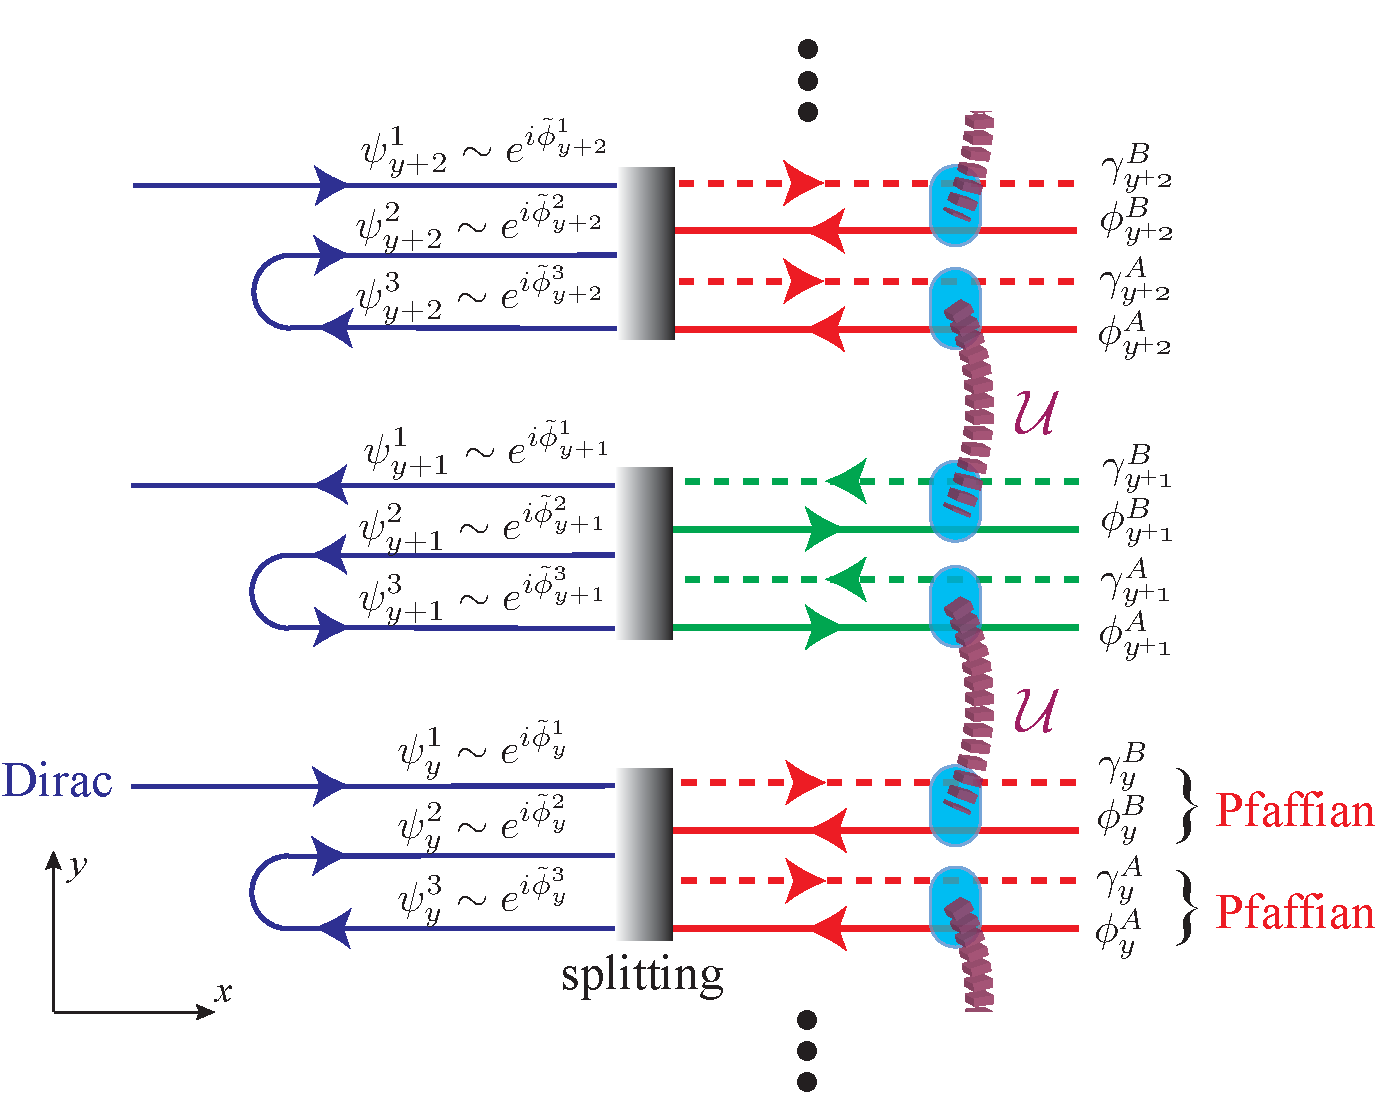
\includegraphics[width=0.9\textwidth]{gappinginteraction2}
	\caption[Symmetry preserving many-body gapping interaction.]{Symmetry preserving many-body gapping interaction. (a) Each {\color{red}$\boldsymbol\times$}/{\color{green}$\bullet$} represents a chiral Pfaffian channel into/out-of paper. Purple dashed line represents many-body gapping interaction $\mathcal{U}$ in \eqref{mbdint}. (b) Coupled wire model on a single layer along the diagonal axis.}\label{fig:gappinginteraction}
\end{figure}

The many-body gapping scheme is summarized in Fig.~\ref{fig:gappinginteraction}. From the previous subsection, we saw that each chiral Dirac channel can be decomposed into a pair of independent Pfaffian channels. They can then be backscattered in opposite directions to neighboring wires. Figure~\ref{fig:gappinginteraction}(a) shows a particular dimerization pattern of the Pfaffian channels that preserves the symmetries. In this case, the many-body backscattering interaction $\mathcal{U}$ is directed along the diagonal axis. In the limit when $\mathcal{U}$ is much stronger than the single-body electron tunneling in the previous semimetallic model \eqref{WeylTBHam}, the system decomposes into decoupled diagonal layers and it suffices to consider the interaction on a single layer. For convenience, we here change our spatial coordinates so that the diagonal axis is now labeled by $y$ and the wires now propagate along $x$.

Focusing on a single diagonal layer, the system in the non-interacting limit first consists of a 2D array of chiral Dirac strings with alternating propagating directions (see the left side of Fig.~\ref{fig:gappinginteraction}(b)). We notice that this is identical to the starting point of the coupled wire construction of the topological insulator Dirac surface state considered by Mross, Essin and Alicea in Ref.~\cite{MrossEssinAlicea15}. For instance, the alternating Dirac channels there were supported between magnetic strips with alternating orientations on the topological insulator surface, and an uniform nearest-channel electron tunneling recovered the massless 2D Dirac spectrum protected by the \AFTR symmetry. They then proceeded to propose symmetry preserving many-body gapping interactions facilitated by adding 2D \FQH strips between the channels. While this reconstruction trick can be applied on the 2D surface of a topological insulator, it is not feasible in our 3D situation and would require drastic modification of the bulk semimetal. Instead, here we propose an alternative gapping scheme that does not involve additional topological phases. In other words, we are going to construct a 3D gapped and layered topological phase solely from interacting electronic Dirac wires.

First, in order to implement the splitting described in the previous subsection, we assume each Dirac string consists of two Dirac channels going in one direction and a third Dirac channel going the opposite direction (see the left side of Fig.~\ref{fig:gappinginteraction}(b)). We denote the electronic Dirac fermions on the $y^{\mathrm{th}}$ wire by $\boldsymbol\psi_y=(\psi_y^1,\psi_y^2,\psi_y^3)$ and bosonize \begin{align}\psi_y^{1,2}(x)\sim e^{i\tilde\phi^{1,2}_y(x)},\quad\psi_y^3(x)\sim e^{-i\tilde\phi^3_y(x)}.\label{bosondef}\end{align} The sliding Luttinger liquid\cite{OHernLubenskyToner99,EmeryFradkinKivelsonLubensky00,VishwanathCarpentier01,SondhiYang01,MukhopadhyayKaneLubensky01} Lagrangian density is \begin{align}\mathcal{L}_{\mathrm{layer}}=\sum_{y=-\infty}^\infty\frac{(-1)^y\tilde{K}_{jk}}{2\pi}\partial_t\tilde\phi_y^j\partial_x\tilde\phi_y^k+\tilde{V}_{jk}\partial_x\tilde\phi_y^j\partial_x\tilde\phi_y^k \,, \label{Llayer}\end{align} where $\tilde{K}=(\tilde{K}_{jk})_{3\times3}=\mathrm{diag}(1,1,-1)$, $\tilde{V}$ is some non-universal velocity matrix, and repeating species indices $j,k$ are summed over. The boson operators obey the equal-time commutation relation (\hypertarget{ETCR}{ETCR}) \begin{align}&\left[\tilde\phi_y^j(x),\tilde\phi_{y'}^{j'}(x')\right]=c^{jj'}_{yy'}(x-x')\nonumber \,, \\=&i\pi(-1)^y\delta_{yy'}\tilde{K}^{jj'}\mathrm{sgn}(x'-x)\label{ETcomm0}\\&+i\pi(-1)^y\delta_{yy'}S^{jj'}\nonumber\\&+i\pi(-1)^{\mathrm{max}\{y,y'\}}\mathrm{sgn}(y-y')\Sigma^{jj'}\sigma_z^{y-y'+1}\nonumber\,, \end{align}
%\begin{align}\left[\tilde\phi_y^j(x),\tilde\phi_{y'}^{j'}(x')\right]=&i\pi(-1)^{\mathrm{max}\{y,y'\}}\Big[\delta_{yy'}\tilde{K}^{jj'}\mathrm{sgn}(x'-x)\nonumber\\&+\delta_{yy'}\mathrm{sgn}(j-j')+\mathrm{sgn}(y-y')\Big]\label{ETcomm0}\end{align} 
where $\mathrm{sgn}(s)=s/|s|=\pm1$ for $s\neq0$ and $\mathrm{sgn}(0)=0$, \begin{align}S=\left(\begin{smallmatrix}0&1&-1\\-1&0&1\\1&-1&0\end{smallmatrix}\right),\quad\Sigma=\left(\begin{smallmatrix}1&1&-1\\1&1&-1\\-1&-1&1\end{smallmatrix}\right),\label{Kleinfactors}\end{align} and $\sigma_z=\pm1$. The introduction of the specific Klein factors $S^{jj'}$, $\Sigma^{jj'}$ and the undetermined sign $\sigma_z$ are necessary for the correct representations of the $\mathcal{T}_{11}$ and $\mathcal{C}_2$ symmetries in the bosonization setting, and these choices will be justified below. The first line of \eqref{ETcomm0} is equivalent to the commutation relation between conjugate fields \begin{align}\left[\tilde\phi_y^j(x),\partial_{x'}\tilde\phi_{y'}^{j'}(x')\right]=2\pi i(-1)^y\delta_{yy'}\tilde{K}^{jj'}\delta(x-x') \,, \label{ETcomm00}\end{align} which is set by the ``$p\dot{q}$" term in $\mathcal{L}_{\mathrm{layer}}$. The alternating signs $(-1)^y$ in \eqref{ETcomm00} and \eqref{Llayer} changes the propagating directions from wire to wire. The second and third line of \eqref{ETcomm0} guarantee the correct anticommutation relations $\{e^{\pm i\tilde\phi^j_y},e^{\pm i\tilde\phi^{j'}_{y'}}\}=0$ between Dirac fermions along distinct channels $j\neq j'$ or distinct wires $y\neq y'$. The reason the $\tilde{C}_2$ matrix is defined in this form will become clear in the fractional basis discussed later in \eqref{bosonC2Pf}.

The anti-unitary \AFTR symmetry along the diagonal $\mathcal{T}_{11}$ direction transforms the bosons according to \begin{align}\mathcal{T}_{11}\tilde\phi^j_y\mathcal{T}_{11}^{-1}=-\tilde\phi^j_{y+1}+\frac{1+(-1)^y}{2}\tilde{K}^{jj}\pi.\label{bosonTR11}\end{align} The unitary $\mathcal{C}_2$ rotation takes \begin{gather}\mathcal{C}_2\tilde\phi^j_y\mathcal{C}_2^{-1}=\left(\tilde{C}_2\right)^j_{j'}\tilde\phi^{j'}_{-y}+(-1)^yv^j\frac{\pi}{2},\label{bosonC2}\\\tilde{C}_2=\left(\begin{smallmatrix}1&2&2\\2&1&2\\-2&-2&-3\end{smallmatrix}\right),\quad{\bf v}=\left(\begin{smallmatrix}v^1\\v^2\\v^3\end{smallmatrix}\right)=\left(\begin{smallmatrix}3\\-3\\1\end{smallmatrix}\right).\nonumber\end{gather} Moreover, we choose the representation so that the sign $\sigma_z$ in the \ETCR \eqref{ETcomm0} is preserved by the \AFTR operator but is flipped by the $C_2$ symmetry, \begin{align}\mathcal{T}_{11}\sigma_z\mathcal{T}_{11}^{-1}=\sigma_z,\quad\mathcal{C}_2\sigma_z\mathcal{C}_2^{-1}=-\sigma_z.\end{align} 

The \ETCR \eqref{ETcomm0} is consistent with the \AFTR symmetry. This means that evaluating $\mathcal{T}_{11}\left[\tilde\phi_y^j(x),\tilde\phi_{y'}^{j'}(x')\right]\mathcal{T}_{11}^{-1}$ by taking the \AFTR operator inside the commutator \begin{align}&\left[\mathcal{T}_{11}\tilde\phi_y^j(x)\mathcal{T}_{11}^{-1},\mathcal{T}_{11}\tilde\phi_{y'}^{j'}(x')\mathcal{T}_{11}^{-1}\right]\nonumber\\&=\left[\tilde\phi_{y+1}^j(x),\tilde\phi_{y'+1}^{j'}(x')\right]=c^{jj'}_{y+1,y'+1}(x-x')\end{align} yields the same outcome as taking the \TR of the purely imaginary scalar \begin{align}\mathcal{T}_{11}c^{jj'}_{yy'}(x-x')\mathcal{T}_{11}^{-1}=-c^{jj'}_{yy'}(x-x').\end{align} The \ETCR \eqref{ETcomm0} is also consistent with the $\mathcal{C}_2$ symmetry \begin{align}(\tilde{C}_2)^{j_1}_{j'_1}c^{j'_1j'_2}_{-y_1,-y_2}(x_1-x_2)(\tilde{C}_2)^{j_2}_{j'_2}=\mathcal{C}_2c^{j_1j_2}_{y_1y_2}(x_1-x_2)\mathcal{C}_2^{-1}.\label{ETcommC2consistent}\end{align} This is because the Klein factors \eqref{Kleinfactors} are $C_2$ symmetric \begin{align}\tilde{C}_2S\tilde{C}_2^T=S,\quad\tilde{C}_2\Sigma\tilde{C}_2^T=\Sigma.\end{align} Notice that the undetermined sign $\sigma_z$, which is odd under $\mathcal{C}_2$, in \eqref{ETcomm0} is essential for the \ETCR to be consistent with $C_2$.

The last term in the \AFTR operation \eqref{bosonTR11} makes sure \begin{align}\mathcal{T}_{11}^2\tilde\phi_y^j(x)\mathcal{T}_{11}^{-2}=\tilde\phi_{y+2}^j+(-1)^y\tilde{K}^{jj}\pi,\end{align} which is necessary for $\mathcal{T}^2_{11}=(-1)^F\mathrm{translation}(2{\bf e}_y)$. Here the fermion parity operator is $(-1)^F=e^{i\pi\sum_{yj}N_y^j}$, where \begin{align}N_y^j=\int\frac{dx}{2\pi}\partial_x\tilde\phi_y^j(x)\label{numop}\end{align} is the number operator. The vector ${\bf v}$ in the $\mathcal{C}_2$ operation \eqref{bosonC2} satisfies $(\delta^j_{j'}+(\tilde{C}_2)^j_{j'})v^{j'}/2=\tilde{K}^{jj}$, and consequently \begin{align}\mathcal{C}_{2}^2\tilde\phi_y^j(x)\mathcal{C}_{2}^{-2}=\tilde\phi_y^j+(-1)^y\tilde{K}^{jj}\pi,\end{align} which is consistent with $\mathcal{C}_2^2=(-1)^F$. Lastly, it is straightforward to check that the symmetry representations \eqref{bosonTR11} and \eqref{bosonC2} are compatible with the algebraic relation \eqref{C2Trelation}, i.e. \begin{align}&\mathcal{C}_2\mathcal{T}_{11}\tilde\phi^j_y\mathcal{T}_{11}^{-1}\mathcal{C}_2^{-1}\\&=(-1)^F\mathcal{T}_{11}^{-1}\mathcal{C}_2\tilde\phi^j_y\mathcal{C}_2^{-1}\mathcal{T}_{11}(-1)^{-F}.\nonumber\end{align}

%The, at first sight, obscured expression of the $3\times3$ rotation matrix $C_2$ in \eqref{bosonC2} actually takes a much simply form under the fractional basis transformation considered in the previous subsection~\ref{sec:gluing}. We defer this simplification a bit later, but at this point, we notice that the Klein fators $S$ and $\Sigma$ in the \ETCR \eqref{ETcomm0} are chosen to be consistent with the $C_2$ symmetry, \begin{align}C_2SC_2^T=S,\quad C_2\Sigma C_2^T=\Sigma.\end{align} 

Following the splitting scheme summarized in Fig.~\ref{fig:fractionalization}, we again define a fractional basis transformation (c.f.~\eqref{fracbasistrans0}) \begin{align}\begin{pmatrix}\phi^\rho_y\\\phi^{\sigma1}_y\\\phi^{\sigma2}_y\end{pmatrix}=\left(\begin{array}{*{20}c}1&1&1\\1&-1/2&1/2\\1&1/2&3/2\end{array}\right)\left(\begin{array}{*{20}c}\tilde\phi^1_y\\\tilde\phi^2_y\\\tilde\phi^3_y\end{array}\right)\label{fracbasistrans}\end{align} for each wire, so that $\psi^\rho_y\sim e^{i\phi^\rho_y}$ is a Dirac fermion carrying electric charge $e$, $d^{\sigma1}_y\sim e^{i\phi^{\sigma1}_y}$ ($d^{\sigma2}_y\sim e^{i\phi^{\sigma2}_y}$) is an electrically neutral Dirac fermion propagating in the same (resp.~opposite) direction as $\psi^\rho_y$.

For convenience, sometimes we combine the transformed bosonized variables into $\boldsymbol\phi_y=(\phi^1_y,\phi^2_y,\phi^3_y)=(\phi^A_y,\phi^B_y,\phi^{\sigma2}_y)$, which is related to the original local ones in \eqref{Llayer} by $\phi^J_y=G^J_j\tilde\phi^j_y$ where \begin{align}G=\begin{pmatrix}1/2&1/8&3/8\\0&3/8&1/8\\1&1/2&3/2\end{pmatrix}.\end{align} The \AFTR symmetry operation \eqref{bosonTR11} becomes \begin{align}\mathcal{T}_{11}\phi^I_y\mathcal{T}_{11}^{-1}=-\phi^I_{y+1}+\frac{1+(-1)^y}{2}\pi\kappa^I\label{bosonTR11Pf}
%\mathcal{T}_{11}\phi^{A/B}_y\mathcal{T}_{11}^{-1}&=-\phi^{A/B}_{y+1}+\frac{1+(-1)^y}{2}\pi,\nonumber\\\mathcal{T}_{11}\phi^{\sigma 2}_y\mathcal{T}_{11}^{-1}&=-\phi^{\sigma 2}_{y+1}.
\end{align} where $\kappa^I=G^I_j\tilde{K}^{jj}$ which is $1/4$ for $I=1,2$ and $0$ for $I=3$. The $C_2$ transformation \eqref{bosonC2} becomes \begin{gather}\mathcal{C}_2\phi^I_y\mathcal{C}_2^{-1}=\left(C_2\right)^I_J\phi^J_{-y}+(-1)^yG^I_jv^j\frac{\pi}{2},\label{bosonC2Pf}\\C_2=G\tilde{C}_2G^{-1}=\left(\begin{smallmatrix}0&1&0\\1&0&0\\0&0&-1\end{smallmatrix}\right),\quad G{\bf v}=\left(\begin{smallmatrix}3/2\\-1\\3\end{smallmatrix}\right).\nonumber\end{gather} The $3\times3$ $C_2$ matrix takes a much simpler form here using the fractional basis than in \eqref{bosonC2}. In fact, the original $\tilde{C}_2$ matrix in the local basis in \eqref{bosonC2} was defined so that $C_2=G\tilde{C}_2G^{-1}$ would act according to \eqref{bosonC2Pf}. Roughly speaking, ignoring the constant phases $G{\bf v}$, the $C_2$ symmetry switches $\phi^A_y\leftrightarrow\phi^B_{-y}$ and sends $\phi^{\sigma2}_y\to-\phi^{\sigma2}_{-y}$.

Next, we combine these co-propagating pair of fermions to form two $SU(2)_1$ current algebras (c.f.~\eqref{SU2current} and \eqref{SU2algebra}) \begin{align}&J_3^{A/B}(y,w)=i2\sqrt{2}\partial_w\phi^{A/B}_y(w)\nonumber \,, \\&J_\pm^{A/B}(y,w)=e^{\pm i4\phi^{A/B}_y(w)} \,, %\\&4\phi^A_y(w)=\phi^\rho_y(w)+\phi^{\sigma1}_y(w),\quad 4\phi^B_y(w)=\phi^\rho_y(w)-\phi^{\sigma1}_y(w)\nonumber
\end{align} where $w\sim\tau+(-1)^yx$ is the complex spacetime parameter. As a reminder, the charge $\pm e$ bosons $J^{A/B}_\pm$ are non-electronic fractional operators, although they carry non-fractional statistics.

The remaining counter-propagating neutral Dirac fermion can be decomposed into real and imaginary components \begin{align}d_y^{\sigma}(w)\sim\cos\phi^{\sigma2}_y(w)+i\sin\phi^{\sigma2}_y(w).\end{align} Majorana fermions can be constructed by multiplying these components with ``Jordan-Wigner" string \begin{align}\gamma^A_y&\sim\cos\phi^{\sigma2}_y\prod_{y'>y}(-1)^{N_{y'}^2+N_{y'}^3},\nonumber\\\gamma^B_y&\sim\sin\phi^{\sigma2}_y\prod_{y'>y}(-1)^{N_{y'}^2+N_{y'}^3},\label{MFdef}\end{align} where $N^j_y$ are the number operators defined in \eqref{numop}, so that they obey mutual fermionic statistics $\{\gamma^\lambda_y(x),\gamma^{\lambda'}_{y'}(x')\}=\delta^{\lambda\lambda'}\delta_{yy'}\delta(x-x')$, for $\lambda,\lambda'=A,B$. Similar to the charge  $\pm e$ bosons $J^{A/B}_\pm$, the electrically neutral Dirac fermion $d_y^\sigma$ and consequently the Majorana fermions $\gamma^{A/B}_y$ are also non-electronic fractional operators. This $AB$-decomposition splits each Dirac wire into a pair of decoupled Pfaffian sectors (see Fig.~\ref{fig:gappinginteraction}(b)).

Before we move on to the symmetric interaction, some further elaborations are needed for the number operators $N_y^j$ and their corresponding fermion parity operators $e^{i\pi N_y^j}$. In our construction, the counter-propagating pair of channels with $j=2,3$ are appended to the original one with $j=1$ to make the Pfaffian fractionalization feasible. We choose the Hilbert space so that the two additional fermion parity operators agree, $e^{i\pi N_y^2}=e^{i\pi N_y^3}$. However, we allow fluctuations to the combined parity $e^{i\pi(N_y^2+N_y^3)}$ and only require it squares to the identity, $e^{2\pi i(N_y^2+N_y^3)}=1$. In other words, $e^{i\pi(N_y^2+N_y^3)}=e^{-i\pi(N_y^2+N_y^3)}$ and it does not matter which one we take as $(-1)^{N_y^2+N_y^3}$ in the ``Jordan-Wigner" string in \eqref{MFdef}. This convention will also be useful later in seeing that the many-body interaction is exactly solvable and symmetry preserving. Extra care is sometimes required. For example, unlike the original Dirac channel where the parity is simply $(-1)^{N_y^1}=e^{\pm i\pi N_y^1}$ because $e^{2\pi iN_y^1}=1$, the individual parity operators $(-1)^{N_y^{2,3}}$ of these additional channels are not well-defined because $e^{2\pi iN_y^{2,3}}\neq1$, i.e.~$e^{i\pi N_y^{2,3}}\neq e^{-i\pi N_y^{2,3}}$. Also, although $e^{2\pi i(N_y^2+N_y^3)}=1$, one cannot in general modify a boson angle parameter simply by $\Theta\to\Theta+2\pi i(N_y^2+N_y^3)$ because $\Theta$ and the number operators may not commute. For instance, using the Baker-Campbell-Hausdorff formula and the \ETCR \eqref{ETcomm0}, $e^{i4\phi^{A/B}}$ and $e^{i4\phi^{A/B}+2\pi i(N_y^2+N_y^3)}$ are off by a minus sign.

The Pfaffian fractionalization is stabilized by the inter-wire many-body backscattering interaction (see Fig.~\ref{fig:gappinginteraction}(b)) \begin{align}\mathcal{U}&=-u\sum_{y=-\infty}^\infty\cos\phi^{\sigma2}_{y+1}\sin\phi^{\sigma2}_y\cos\left(4\phi^A_{y+1}-4\phi^B_y\right)\nonumber \,,\\
&=-u\sum_{y=-\infty}^\infty(-1)^yi\gamma^A_{y+1}\gamma^B_y\cos\left(\Theta_{y+1/2}\right),\label{mbdint}\end{align} for $\Theta_{y+1/2}(x)=4\phi^A_{y+1}(x)-4\phi^B_y(x)+\pi(N_{y+1}^2+N_{y+1}^3)$. Previously in \eqref{psi4def1}, we saw that the combinations $\psi_4^A\sim e^{i4\phi^A}\gamma^A$ and $\psi_4^B\sim e^{i4\phi^B}\gamma^B$ can be decomposed into products of electron operators. Similarly, each interaction in the first line of \eqref{mbdint} can be decomposed into products in the form of $e^{\pm i(\phi^{\sigma2}_{y+1}\pm4\phi^A_{y+1})}e^{\pm i(\phi^{\sigma2}_y\pm4\phi^B_y)}$ (with some scalar $U(1)$ coefficient), where the exponents $\phi^{\sigma2}\pm4\phi^{A/B}$ are linear integral combinations of $\tilde\phi^j$. Thus, the interaction can be re-written in terms of backscatterings of local electronic operators. However, we will omit the electronic expression as \eqref{mbdint} is more useful in discussing ground state and symmetries. 

$\mathcal{U}$ describes a symmetry-preserving exactly solvable model. Using the \ETCR \eqref{ETcomm0} it is straightforward to check that the (normal ordered) order parameters \begin{align}\mathcal{O}_{y+1/2}^F(x)=i\gamma^A_{y+1}(x)\gamma^B_y(x),\quad\mathcal{O}_{y+1/2}^\Theta(x)=e^{i\Theta_{y+1/2}(x)}\label{orderparameters}\end{align} mutually commute, i.e. $\left[\mathcal{O}_{y+1/2}^{F/\Theta}(x),\mathcal{O}_{y'+1/2}^{F/\Theta}(x')\right]=0$. Therefore, the model is exactly solvable, and its ground states are characterized by the ground state expectation values (\hypertarget{GEV}{GEV}) of the order parameters \begin{align}l_0\langle\mathcal{O}_{y+1/2}^F\rangle=(-1)^y\langle\mathcal{O}_{y+1/2}^\Theta\rangle=\pm1 \,, \end{align} so that the interacting energy $\langle\mathcal{U}\rangle$ is minimized, where $l_0$ is some non-universal microscopic length scale. Pinning the \GEV $\langle\Theta_{y+1/2}\rangle=n_{y+1/2}\pi$, for $n_{y+1/2}\in\mathbb{Z}$, gaps all degrees of freedom in the charged $U(1)_4^{A/B}=SU(2)_1^{A/B}$ sector. The remaining neutral fermions are gapped by the decoupled Majorana backscattering \begin{align}\delta\mathcal{H}_{\mathrm{Majorana}}=u\sum_{y=-\infty}^\infty(-1)^yi\langle\mathcal{O}^\Theta_{y+1/2}\rangle\gamma^A_{y+1}\gamma^B_y.\label{MajHam}\end{align} It is worth noting that a $\pi$-kink excitation of $\langle\Theta_{y+1/2}\rangle$ flips the Majorana mass in \eqref{MajHam} and therefore bounds a zero energy Majorana bound state~\cite{Kitaevchain}. A $\pi$-kink at $x_0$ can be created by the vertex operators $e^{\pm i\phi^A_{y+1}(x_0)}$ or $e^{\pm i\phi^B_y(x_0)}$ which carry $\pm1/4$ of an electric charge. (Recall the bosonic vertices $e^{i4\phi^{A/B}_y}$ carry charge $e$.) This $e/4$ excitation therefore corresponds to the Ising anyon in the Pfaffian \FQH state.

From the \AFTR symmetry action \eqref{bosonTR11Pf}, one can show that the Majorana fermions \eqref{MFdef} transform according to \begin{align}\mathcal{T}_{11}\gamma^A_y\mathcal{T}_{11}^{-1}=\gamma^A_{y+1},\quad\mathcal{T}_{11}\gamma^B_y\mathcal{T}_{11}^{-1}=-\gamma^B_{y+1}.\end{align} Therefore the fermion order parameter $\mathcal{O}^F_{y+1/2}=i\gamma^A_{y+1}\gamma^B_y$ \eqref{orderparameters} is translated under the antiunitary symmetry \begin{align}\mathcal{T}_{11}\mathcal{O}^F_{y+1/2}\mathcal{T}_{11}^{-1}=\mathcal{O}^F_{y+3/2}.\label{T11OF}\end{align} The boson angle parameter $\Theta_{y+1/2}$ defined below \eqref{mbdint} changes to $-\Theta_{y+3/2}-(-1)^y\pi$ under \AFTR, and therefore the boson order parameter $\mathcal{O}^\Theta_{y+1/2}=e^{i\Theta_{y+1/2}}$ is flipped and translated \begin{align}\mathcal{T}_{11}\mathcal{O}^\Theta_{y+1/2}\mathcal{T}_{11}^{-1}=-\mathcal{O}^\Theta_{y+3/2}.\label{T11OT}\end{align} Together, \eqref{T11OF} and \eqref{T11OT} show that the many-body interaction $\mathcal{U}$ in \eqref{mbdint} is \AFTR symmetric.

The $C_2$ action \eqref{bosonC2} flips the number operator $\mathcal{C}_2(N_y^2+N_y^3)\mathcal{C}_2^{-1}=-N_{-y}^2-N_{-y}^3$, and therefore the parity operators appear in the ``Jordan-Wigner" string \eqref{MFdef} are $C_2$ symmetric, $\mathcal{C}_2(-1)^{N_y^2+N_y^3}\mathcal{C}_2^{-1}=(-1)^{N_{-y}^2+N_{-y}^3}$. With the help of the $C_2$ action \eqref{bosonC2Pf} in the fractional basis, one sees that $\mathcal{C}_2\cos\phi^\sigma_y\mathcal{C}_2^{-1}=(-1)^{y+1}\sin\phi^\sigma_{-y}$ and $\mathcal{C}_2\sin\phi^\sigma_y\mathcal{C}_2^{-1}=(-1)^{y+1}\cos\phi^\sigma_{-y}$ and thus the Majorana fermions \eqref{MFdef} transform according to \begin{align}\mathcal{C}_2\gamma^A_y\mathcal{C}_2^{-1}=(-1)^{y+1}\gamma^B_{-y}(-1)^{F_{2+3}},\\\mathcal{C}_2\gamma^B_y\mathcal{C}_2^{-1}=(-1)^{y+1}\gamma^A_{-y}(-1)^{F_{2+3}},\nonumber\end{align} where $(-1)^{F_{2+3}}=\prod_{y=-\infty}^\infty(-1)^{N_y^2+N_y^3}$ is the total fermion parity of channel 2 and 3. This shows the fermion order parameter is odd under $C_2$ \begin{align}&\mathcal{C}_2\mathcal{O}^F_{y+1/2}\mathcal{C}_2^{-1}\nonumber\\&=i(-1)^{y+2}\gamma^B_{-y-1}(-1)^{F_{2+3}}(-1)^{y+1}\gamma^A_{-y}(-1)^{F_{2+3}}\nonumber\\&=-i\gamma^A_{-y}\gamma^B_{-y-1}=-\mathcal{O}^F_{-y-1/2}.\label{C2OF}\end{align} On the other hand, one can also show from the $C_2$ action \eqref{bosonC2Pf} that the boson angle parameter changes as $\mathcal{C}_2\Theta_{y+1/2}\mathcal{C}_2^{-1}=-\Theta_{-y-1/2}-(-1)^y\pi$ and therefore the boson order parameter $\mathcal{O}^\Theta_{y+1/2}=e^{i\Theta_{y+1/2}}$ is conjugated and flipped under $C_2$ \begin{align}\mathcal{C}_2\mathcal{O}^\Theta_{y+1/2}\mathcal{C}_2^{-1}=-{\mathcal{O}^\Theta_{-y-1/2}}^\dagger.\label{C2OT}\end{align} When combined together, the minus signs in \eqref{C2OF} and \eqref{C2OT} cancel and they show that the many-body interaction $\mathcal{U}$ in \eqref{mbdint} preserves $C_2$.

Now that we have introduced symmetry preserving gapping interactions on a single diagonal layer, we can extend it to the entire 3D structure by transferring \eqref{mbdint} to all layers using the off-diagonal \AFTR operator $\mathcal{T}_{\bar{1}1}$ (see Fig.~\ref{fig:gappinginteraction}(a)). The resulting state belongs to a topological phase in three dimensions with an excitation energy gap. It preserves both \AFTR symmetries $\mathcal{T}_{11}$ and $\mathcal{T}_{\bar{1}1}$ as well as the (screw) $C_2$ symmetry. The choice of writing this dissertation with a specific model with these symmetries was intentional, we wanted to work out the simplest example with specific symmetries explicitly for illustrative reasons instead of doing a more general classification type argument. We leave the SPT-SET correspondences for general symmetries as an open question, but we expect that the methods presented in this work can be useful in exploring them.


\subsection{Antiferromagnetic stabilization}\label{sec:AFMstabilization}
The exactly-solvable many-body interacting model \eqref{mbdint} (see also Fig.~\ref{fig:gappinginteraction}) shows that the Dirac semimetal \eqref{WeylTBHam} can acquire a many-body mass gap without breaking symmetries. However, it is not clear how dominant or stable the topological phase described by \eqref{mbdint} is. There are alternative interactions that lead to other metallic or insulating phases that preserve or break symmetries. The scaling dimensions and the relevance of the interaction terms~\cite{Fradkinbook,Tsvelikbook} can be tuned by the velocity matrix $V_{jk}$ in \eqref{Llayer} that is affected by forward scattering interactions among co-propagating channels. Instead of considering energetics, we focus on a topological deliberation -- inspired by the coupled wire construction of quantum Hall states~\cite{KaneMukhopadhyayLubensky02,TeoKaneCouplewires} -- that can drastically reduce the number of possible interactions and may stabilize the desired interactions when applied to materials.

The coupled wire model considered so far assumes all electronic Dirac modes at the Fermi level have zero momentum $k_x=0$. This is convenient for the purpose of constructing an exactly solvable model because momentum is automatically conserved by the backscattering interactions. However, this also allows a huge collection of competing interactions. We propose the application of a commensurate modulation of magnetic field to restrict interactions that conserve momentum. There are multiple variations to the application, which depend on the details of the Dirac material and the Dirac vortices. To illustrate the idea, we present one possible simple scenario.

\begin{figure}[htbp]
	\centering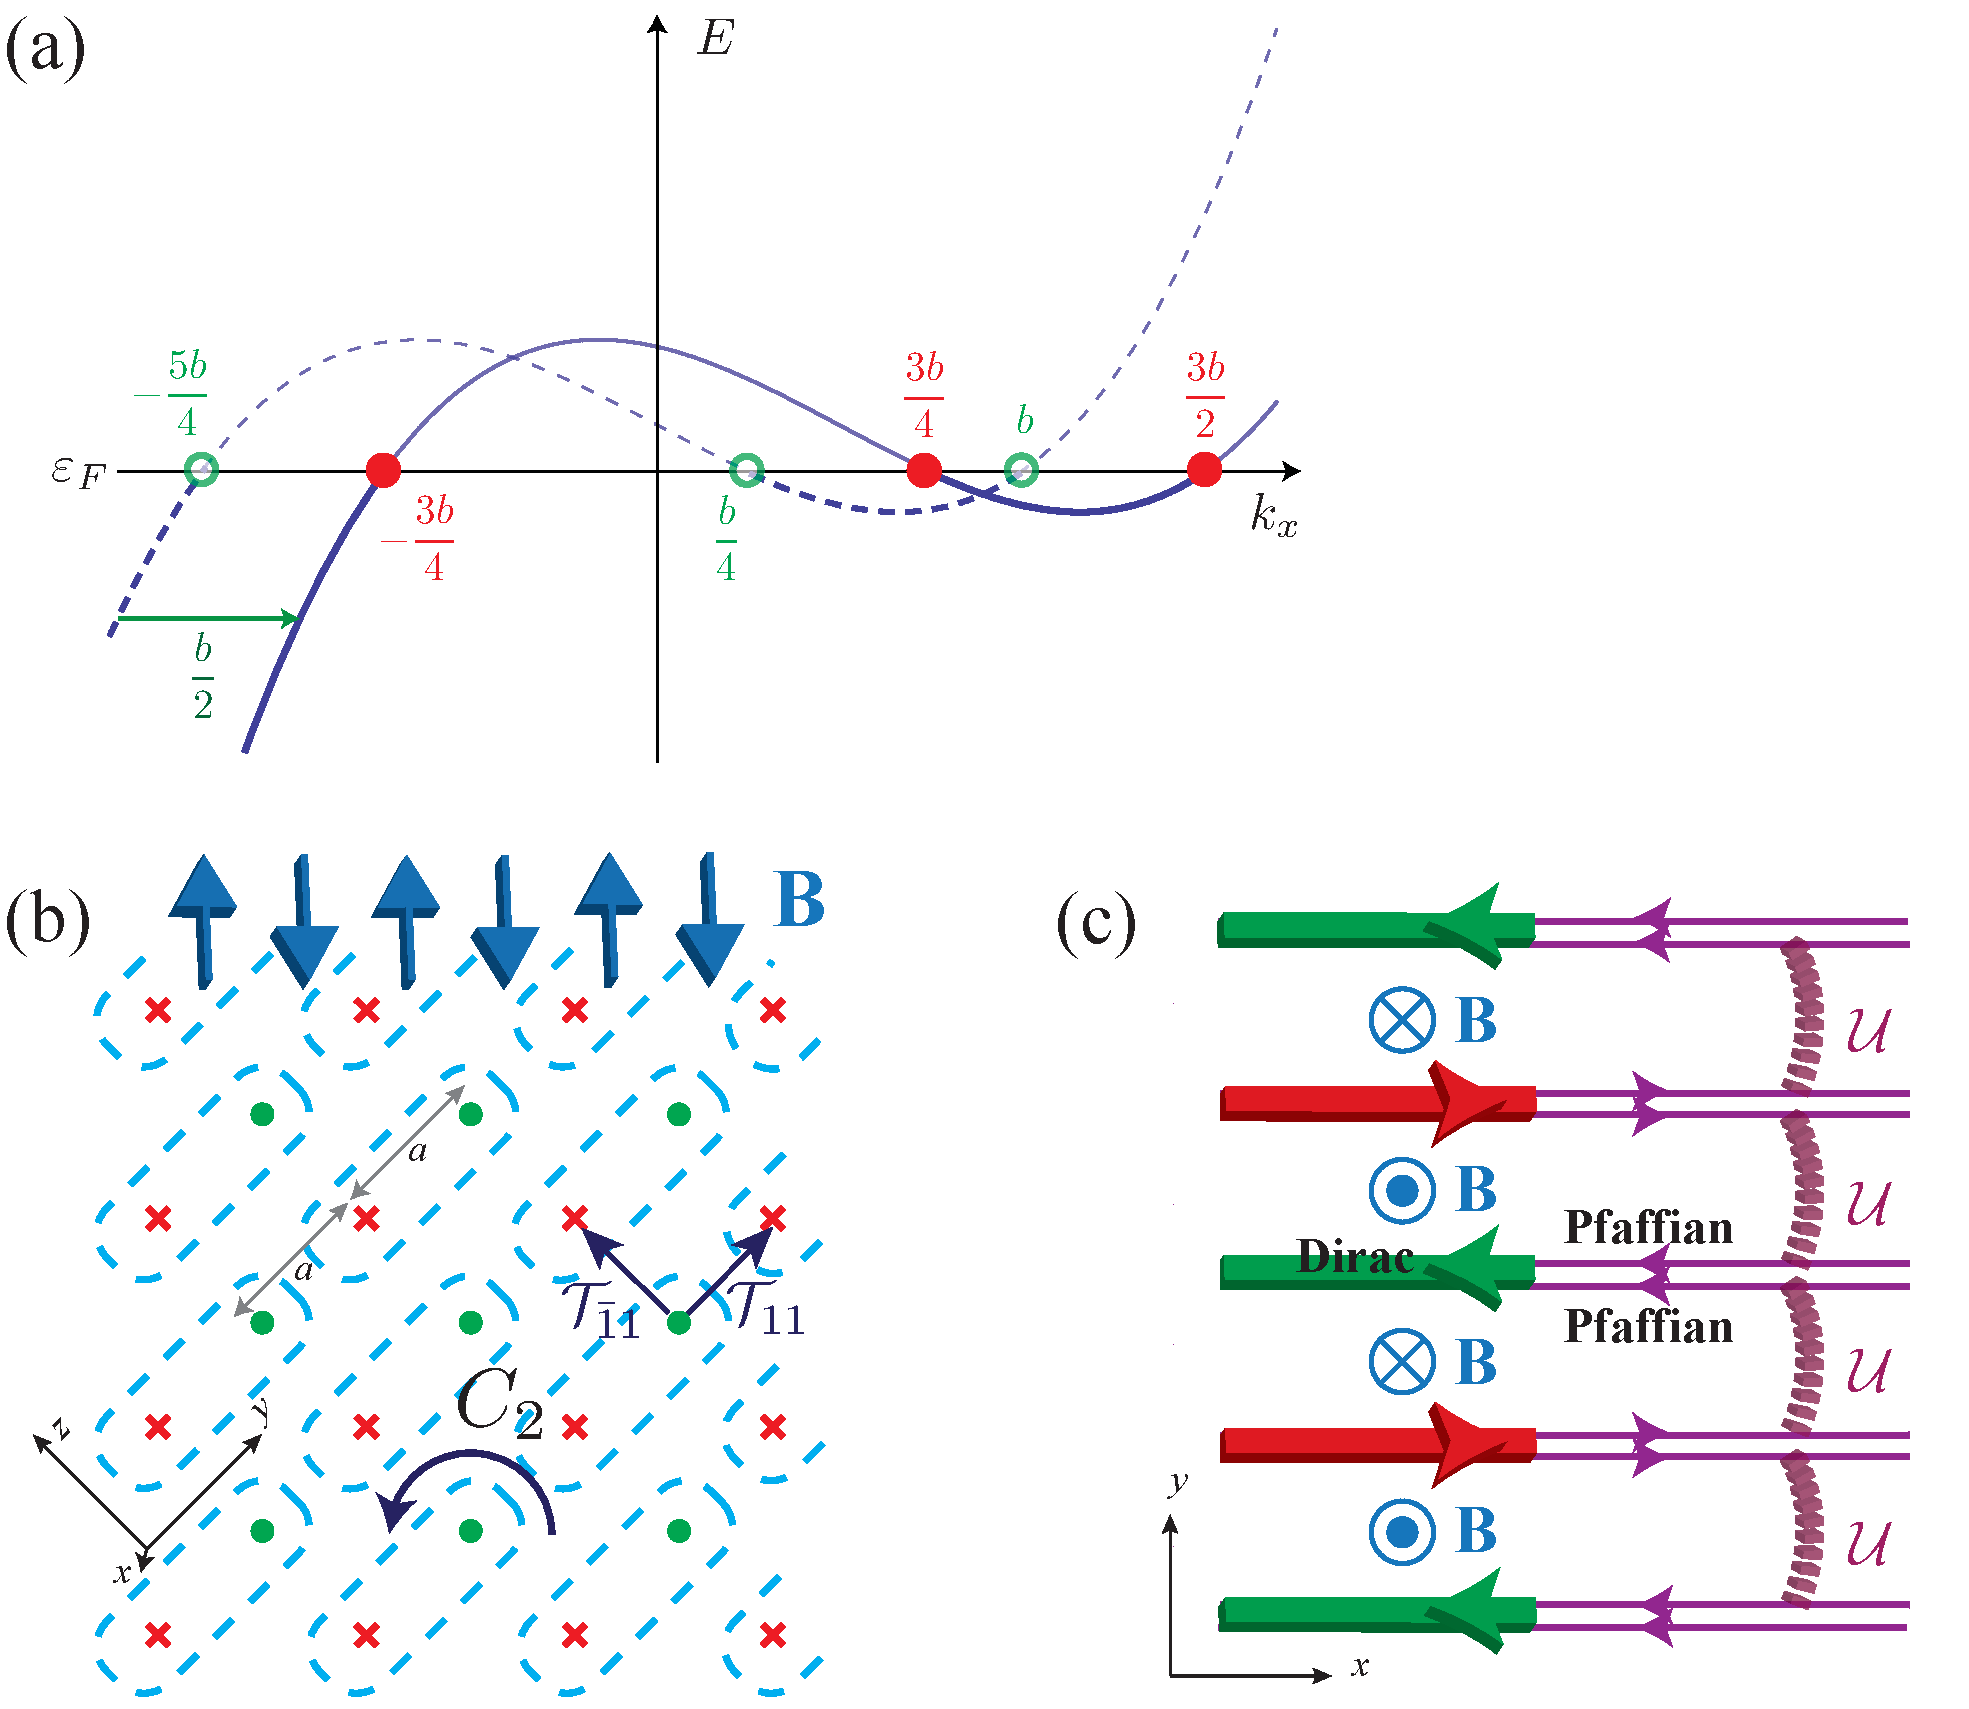
\includegraphics[width=0.9\textwidth]{afm}
	\caption[Antiferromagnetic stabilization.]{(a) The energy dispersion $E_{y=2l}(k_x)$ with (solid curve) or without (dashed curve) the alternating magnetic field. (b) The alternating magnetic field configuration that preserves the AFTR and $C_2$ symmetries. (c) The alternating magnetic field across a single layer along the $xy$ plane.}\label{fig:afm}
\end{figure}

First we go back to a single Dirac wire and consider a non-linear dispersion \begin{align}E^0_{y=2l}(k_x)&=\frac{\hbar v}{b^2}(k_x-k_F^1)(k_x-k_F^2)(k_x-k_F^3),\nonumber\\E^0_{y=2l+1}(k_x)&=-\frac{\hbar v}{b^2}(k_x+k_F^1)(k_x+k_F^2)(k_x+k_F^3),\end{align} where $v$ and $b$ are some non-universal velocity and wave number parameters. We assume $k_F^2<k_F^3<k_F^1$ so that when the Fermi energy is at $\varepsilon_F=0$, there are two right (left) moving modes at $k_x=k_F^1,k_F^2$ and one left (resp.~right) moving one at $k_X=k_F^3$ along an even (resp.~odd) wire. This matches the three-channel Dirac wire \eqref{3Dirac} used in the splitting scheme in Sec.~\ref{sec:gluing}. We assume the three Fermi wave numbers satisfy a commensurate condition \begin{align}2k_F^1+k_F^2-3k_F^3=0,\label{kcomm}\end{align} and we set \begin{align}b=2(k_F^3-k_F^1-k_F^2).\label{bcomm1}\end{align} The dashed band in Fig.~\ref{fig:afm}(a) shows one commensurate energy dispersion along an even wire.

Next, we consider a spatially modulating magnetic field ${\bf B}({\bf r})=B({\bf r}){\bf e}_{11}$, where \begin{align}B({\bf r})=\sum_{m=-\infty}^\infty B_m\sin\left[\pi\frac{\sqrt{2}(2m+1)}{a}{\bf e}_{\bar{1}1}\cdot{\bf r}\right],\end{align} ${\bf e}_{11}=({\bf e}_y+{\bf e}_z)/\sqrt{2}$ and ${\bf e}_{\bar{1}1}=(-{\bf e}_y+{\bf e}_z)/\sqrt{2}$, that preserves both the \AFTR and $C_2$ symmetries, \begin{align}B({\bf r}+a{\bf e}_y)=B({\bf r}+a{\bf e}_z)=B(C_2{\bf r})=-B({\bf r})\end{align} (see Fig.~\ref{fig:afm}(b) for the 3D field configuration). Moreover, we assume the field is commensurate with the Fermi wave numbers so that the magnetic flux per unit length across the $xy$ layer between adjacent wires (see Fig.~\ref{fig:afm}(c)) is \begin{align}\frac{\Phi_B}{L}=\frac{\phi_0}{2\pi}b \,, \label{bcomm2}\end{align} where $L$ is the wire length, $\phi_0=hc/e$ is the magnetic flux quantum. Equivalently, the average magnetic field strength in the normal $z$-direction between adjacent wires is $|\overline{B_z}|=|\overline{B}|/\sqrt{2}=(\hbar c/ea)b$, where $a$ is the displacement between adjacent counter-propagating wires. We choose the vector potential $A_x(y,z)=[(-1)^y+(-1)^z-1]|\overline{B_z}|a/2$ and $A_y=A_z=0$ along the $(y,z)^{\mathrm{th}}$ wire. 

Along a wire on the $xy$ plane where $z=0$, the three electronic Dirac channels are now bosonized by \begin{align}\psi_y^{1,2}(x)&\sim e^{i[(-1)^y(k_F^{1,2}x+bx/2)+\tilde\phi_y^{1,2}(x)]},\\\psi_y^3(x)&\sim e^{i[(-1)^y(k_F^3x+bx/2)-\tilde\phi_y^3(x)]},\nonumber\end{align} where the momenta are shifted by $k_F^j\to k_F^j+(e/\hbar c)A_x$. The phase oscillation $e^{ikx}$ is canceled in an interaction term only when momentum is conserved, or otherwise the interaction would drop out after the integration over $x$. It is straightforward to check that the Majorana fermions \eqref{MFdef}, which contain the operators $e^{\pm i\phi^\sigma}$, have zero momentum because of the Fermi wave number commensurate condition \eqref{kcomm}. In addition, the boson backscattering $\cos(4\phi^A_{y+1}-4\phi^B_y)$ in \eqref{mbdint} preserves momentum because the magnetic field is also commensurate (see \eqref{bcomm1} and \eqref{bcomm2}).


%
\chapter{Model 2: Dirac Nodal Superconductor}\label{chap:Model2}
\section{Introduction}
Soon after the discovery of the topological band insulators\cite{RevModPhys.82.3045,RevModPhys.83.1057}, generalizing the topological phases to various materials has been one of the most popular themes in condensed matter physics\cite{RevModPhys.88.035005,doi:10.1002/pssr.201206451,doi:10.1146/annurev-conmatphys-031214-014749,doi:10.1146/annurev-conmatphys-031214-014501}. One intensively considered path of extending the topological phases is to consider the topological properties of semimetallic phases. Topological semimetallic phases possess a bulk degeneracy that is protected by the presence of an underlying topology. Up to now, the $3D$ topological semimetals are largely classified into the two classes: Weyl semimetals and Dirac semimetals. Weyl semimetals have two-fold linear band crossings and generally come in two interconnected varieties, namely type-1 and type-2. Type-1 Weyl semimetals have  either broken time-reversal or inversion symmetry and have been found in non-centrosymmetric materials such as: $\mathrm{TaAs}$\cite{PhysRevX.5.031013}, $\mathrm{TaP}$, $\mathrm{NbP}$, and $\mathrm{NbAs}$\cite{Liu2015,Xu2015}. Type-2 Weyl semimetals possess an additional broken Lorentz invariance and both $\mathrm{MoTe_2}$\cite{MoTe,MoTe2} and $\mathrm{WTe_2}$\cite{WTe,WTe2} are observed to be the type-2 Weyl semimetals\cite{type2}. Weyl semimetals have been predicted to have numerous distinguishing physical responses related to the presence of the chiral anomaly\cite{PhysRev.177.2426,Bell1969,Nielsen1983}. Examples of anomalous behavior in Weyl semimetals include: nonlocal quasiparticle transport\cite{PhysRevX.4.031035}, chiral magnetic effect\cite{Li2016,PhysRevB.92.161110,PhysRevB.89.081407}, chiral vortical effect\cite{PhysRevB.89.075124}, angular dependence of the magenetoresistence\cite{PhysRevX.5.031023,PhysRevB.88.104412}.

Unlike the Weyl semimetals, the Dirac semimetals have four-fold degeneracy and require additional symmetries for the topological protection of the gapless bulk Dirac point. Most Dirac semimetals are found in non-magnetic materials such as $\mathrm{Na_3Bi}$\cite{Liu864,PhysRevB.85.195320,Liu864,Xu294,Xiong413} and $\mathrm{Cd_3 As_2}$\cite{Liu2014,PhysRevB.88.125427,Neupane2014,PhysRevLett.113.027603,Jeon2014,Liang2014,PhysRevLett.113.246402,PhysRevLett.115.226401,PhysRevB.92.081306,Li2015,Li2016,Guo2016,Zhang2017}, that preserve both time-reversal symmetry and inversion symmetry. Recently, the discovery of the Dirac semimetals has been extended to include the antiferromagnetic material $\mathrm{CuMnAs}$ that breaks both inversion and time-reversal symmetries yet preserves the product of the two\cite{Tang2016}. As is the case with Weyl semimetals, Dirac semimetals are predicted to possess physical manifestations that are separate and distinct from those found in Weyl semimetals or a $\mathbb{Z}_2$ anomaly\cite{PhysRevLett.117.136602,Xiong413}.

The study of the gapless topological phases can be further generalized into the class of superconducting states, often referred to as topological nodal superconductors\cite{PhysRevB.90.205136,1367-2630-15-6-065001,PhysRevLett.110.240404,0953-8984-27-24-243201}. The topological nodal superconductors are the superconducting analogue of the topological semimetals. The topological nodal superconductors possess nodal points or lines in the Brillouin zone(BZ), which has the vanishing superconducting gap. There has been numerous experimental and theoretical studies of the line nodal superconductors such as noncentrosymmetric superconductors including: $\mathrm{CePt_3Si}$\cite{PhysRevLett.94.207002,PhysRevLett.94.197002}, $\mathrm{Li_2Pt_3B}$\cite{PhysRevLett.97.017006}, and $\mathrm{CeIrSi_3}$\cite{PhysRevLett.100.107003}, and the heavy fermion compounds, $\mathrm{UBe_{13}}$\cite{PhysRevLett.52.1915}. Point nodal superconductors, often referred to as Weyl superconductors, are also proposed to exist in a veritable plethora of materials and systems including: $\mathrm{A}$ phase of $\mathrm{^{3}He}$\cite{RevModPhys.47.415,Volovik2011,volovik}, topological insulator-superconductor multilayers\cite{PhysRevB.86.054504}, doped Weyl semimetals\cite{PhysRevLett.120.067003,PhysRevB.86.214514,PhysRevB.92.035153,Huang2017,PhysRevB.93.184511}, the $\mathrm{B}$ phase of $\mathrm{UPt_3}$\cite{PhysRevB.92.214504}, the pnictide material $\mathrm{SrPtAs}$ \cite{PhysRevB.89.020509}, ferromagnetic superconductors\cite{PhysRevB.86.104509}, the superfluidity of Fermi gases\cite{PhysRevLett.115.265304,PhysRevLett.114.045302}, mirror symmetric superconductors\cite{PhysRevB.97.060504}, the half-metal/$d$-wave superconductor heterostructure\cite{PhysRevB.95.064513}, $\mathrm{Nb}$-doped $\mathrm{Bi_2Se_3}$\cite{PhysRevB.94.180510,PhysRevB.95.201109,PhysRevB.95.201110}, the $\mathrm{Cu}$-doped $\mathrm{Bi_2Se_3}$\cite{PhysRevB.96.144512,PhysRevB.94.180504,PhysRevLett.113.046401}, $\mathrm{PrOs_4Sb_{12}}$\cite{PhysRevLett.90.117001,PhysRevB.76.054514,ABUALRUB20081178}. $\mathrm{Cu_xBi_2Se_3}$ has been predicted to have the four-fold degenerate Dirac points, which is known as the Dirac superconductor\cite{PhysRevLett.113.046401}. As is evidenced in the above listed examples, topological nodal superconductors are often found in the strongly-correlated materials since the anisotropic pairing symmetries in the unconventional superconductors naturally introduces the nodal structures of the superconducting gap\cite{0953-8984-27-24-243201}. Therefore, it is crucial to study the strongly correlated phases of the nodal superconductors to fully understand the physical behavior of these materials.

In this regard, we study the superconductor analogue of the Dirac semimetals, namely Dirac nodal superconductors, in the presence of many-body interactions. To do so, we utilize the coupled wire construction method. In the coupled wire construction, the two and three dimensional phases of matter can be constructed by assembling an array of one dimensional wires. In this method, the many-body interactions are treated between neighboring wires, thereby it enables us to use the theoretical techniques that are only available in one dimension. This method has successfully reproduced and identified elementary excitations and behaviors of the numerous topological phases. In the two dimensional materials, the examples include the Laughlin states\cite{PhysRevLett.50.1395} and the hierarchy states\cite{PhysRevLett.51.605} of the fractional quantum Hall phases\cite{PhysRevLett.88.036401}, general Abelian and non-Abelian fractional quantum Hall phases\cite{PhysRevB.89.085101,PhysRevX.7.031009,Klinovaja2014,Meng2014}, fractional helical liquid{\cite{PhysRevB.89.115402}}, $2D$ fractional topological insulators\cite{PhysRevB.90.205101,PhysRevB.90.115426,PhysRevB.90.201102,PhysRevB.91.205141,PhysRevX.5.011011}, topological superconductors\cite{PhysRevX.4.011036,PhysRevB.89.104523} the surface of fractional topological insulator\cite{PhysRevB.90.201102,PhysRevX.5.011011}, and the spin-liquids\cite{PhysRevB.91.241106,PhysRevB.94.195130,PhysRevB.91.245139}.
The studies of the coupled wire construction even extend to the three-dimensional materials including $3D$ fractional topological phases\cite{PhysRevB.92.195137,PhysRevB.93.195136,Iadecola2017}, interacting Weyl semimetals\cite{PhysRevB.94.155136,0295-5075-102-6-67011,PhysRevB.92.115152,Mross}, the surface of $3D$ topological superconductor\cite{PhysRevB.94.165142}, and interacting Dirac semimetals\cite{Raza2017}.


\section{Coupled Wire Models of Dirac Nodal Superconductor}\label{sec:coupled}
In this section, we describe the single-body aspects of the Dirac nodal superconductor in terms of a coupled wire model. This mirrors the discussions of the non-interacting model in ref.~\cite{RazaSirotaTeo17}. The major difference between our work and previous implementations of the coupled wire constructions of topological phenomena is that in this work we focus on superconducting media that break charge $U(1)$ conservation. The basic building blocks of the coupled wire model are chiral Dirac wires. These are $(1+1)$-D Dirac fermion channels where quasiparticles can only propagate in a single direction. They can be supported by an array of vortices in a degenerate point nodal superconductor in the continuum model. In our model, the nodal superconducting state has a normal metallic parent state that is quasi-one-dimensional with dispersion predominantly in the $y$-direction and pairing order that is $p$-wave directed along the normal $xz$-plane. The Hamiltonian of the nodal superconductor in the continuum limit is given as,
\begin{align}
H_{\mathrm{SC-nodal}}({\bf k})&=(\hbar vk_ys_y\mu_z-\epsilon_f)\tau_z\nonumber\\&\;\;\;\;+\Delta l(\tilde{k}_xs_z-\tilde{k}_zs_x)\mu_x\tau_x,
\label{DiracNODAL}
\end{align}
and is acting on the Nambu vector $\boldsymbol\xi=({\bf c},is_y{\bf c}^\dagger)^T$, where ${\bf c}=(c_{s\mu})$ are the (complex) Dirac fermion annihilation operators, and $s=\uparrow,\downarrow$ and $\mu=\pm$ are the Pauli matrices for the spin and Weyl-species degrees of freedom respectively. In addition, $\vec\tau=(\tau_x,\tau_y,\tau_z)$ are Pauli matrices acting on the Nambu $(c,c^\dagger)$ degree of freedom.

The model in Eq. \eqref{DiracNODAL} can be further simplified by the unitary basis transformation, $U=(\tau_z+s_y\mu_y\tau_x)/\sqrt{2}$ when the momenta are rescaled so that $\Delta l\tilde{k}=\hbar vk$, and the Fermi energy is set at $\epsilon_f=0$. Under these aforementioned conditions, we define a new, simplified superconducting Hamiltonian $H_{\mathrm{SC-Dirac}}=UH_{\mathrm{SC-nodal}}U^{-1}$, written explicitly as,
\begin{align}
H_{\mathrm{SC-Dirac}}({\bf k})=\hbar v{\bf k}\cdot\vec{s}\mu_z\tau_z,
\label{DiracSC}
\end{align}
where $\vec{s}=(s_x,s_y,s_z)$ are Pauli spin matrices and $\mu_z=\pm1$ indexes the two Weyl species with opposite Chern numbers.

The BdG Hamiltonian in Eq. \eqref{DiracSC} has the time-reversal symmetry,
\begin{align}
s_yH_{\mathrm{SC-Dirac}}({\bf k})^\ast s_y=H_{\mathrm{SC-Dirac}}(-{\bf k}),
\label{DiracNODALHTR}
\end{align} and the particle-hole symmetry $s_y\tau_yH({\bf k})^\ast s_y\tau_y=-H(-{\bf k})$ due to the Nambu doubling. In addition, we consider the effective mirror glide symmetry,
\begin{align}
s_z\tau_yH_{\mathrm{SC-Dirac}}({\bf k})s_z\tau_y=H_{\mathrm{SC-Dirac}}(M{\bf k}),
\label{DiracNODALHglide}
\end{align}
where $M:(k_x,k_y,k_z)\to(k_x,k_y,-k_z)$. The mirror-glide $G=s_z\tau_y$ is consistent with the Nambu doubling as it commutes with the particle-hole operator $\Xi=s_y\tau_y\mathcal{K}$, where $\mathcal{K}$ is the complex conjugation operator. The mirror glide $G$ and time-reversal $T=is_y\mathcal{K}$ also mutually commute. While a symmorphic mirror operator squares to $-1$ in a spinful system, a nonsymmorphic glide operator squares to $-e^{iK\cdot{\bf a}}$, where ${\bf a}$ is a microscopic in-plane lattice translation. In our model, we assume the Dirac degeneracy sits at the microscopic lattice momentum $K$ so that $e^{iK\cdot{\bf a}}=-1$, and the Hamiltonian \eqref{DiracNODAL} describes the small momentum deviation ${\bf k}$ away from $K$ in the long length-scale limit ${\bf a}\to0$. The time-reversal and particle-hole operator are unaltered by the basis transformation, $U$, but the glide symmetry changes from $G=-s_x\mu_y$ to $G=-s_z\tau_y$. For mathematical convenience, we will utilize the non-electronic basis where the BdG Hamiltonian is Eq. \eqref{DiracSC} and $G=s_z\tau_y$.

The time-reversal and particle-hole symmetry allow the gap-opening mass terms $\Delta\mu_z\tau_x+m_1\tau_x+m_2\mu_x\tau_z$ but neither of these terms preserves the glide symmetry. We notice in passing that these glide breaking mass terms can lead to a set of interesting topological superconducting states in the Altland-Zirnbauer DIII class~\cite{AltlandZirnbauer97}. A non-vanishing energy gap arises when $|\Delta|\neq\sqrt{m_1^2+m_2^2}$ and there are three disconnected regions separated by the condition where $|\Delta|=\sqrt{m_1^2+m_2^2}$. The two disconnected regions defined by $\Delta>\sqrt{m_1^2+m_2^2}$ and $\Delta<-\sqrt{m_1^2+m_2^2}$ are occupied by time-reversal symmetric topological superconductors~\cite{Ryu2008,Kitaevtable08} with topological indices $N=1$ and $-1$ respectively. The remaining region $|\Delta|<\sqrt{m_1^2+m_2^2}$ is path-connected and is occupied by trivial superconductors with topological index $N=0$. However, the region $|\Delta|<\sqrt{m_1^2+m_2^2}$ is not simply-connected. There is a fundamental homotopy group $\pi_1=\mathbb{Z}$, which classifies vortices of $m({\bf r})=m_1({\bf r})+im_2({\bf r})=|m|e^{i\varphi({\bf r})}$ where the phase $\varphi({\bf r})$ spatially modulates and winds $2\pi n$ around a vortex. A vortex line hosts $n$ pairs of helical Majorana fermions modes, which are protected by time-reversal symmetry when $n$ is odd.


We now restrict our model to be the mirror glide symmetric. The nodal superconducting Dirac state in Eq. \eqref{DiracSC} is stable in the single-body setting and is protected by time-reversal symmetry, $T$, and mirror-glide symmetry, $G$. This can be verified by explicitly checking that there are no symmetry-preserving gap-opening mass terms. Alternatively, this can also be explained using topological reasoning that does not require the specific form of the Hamiltonian. Let us begin by focusing on the mirror-glide symmetric $k_x-k_y$ plane where $k_z=0$. Along this plane, the BdG Hamiltonian commutes with the mirror-glide operator $G=s_z\tau_y$ and, thus, can be block diagonalized according to the corresponding mirror-glide eigenvalues $g=\pm1$. Since $G$ commutes with both time-reversal symmetry and particle-hole symmetry, each mirror sector also carries the same symmetries.  Each sector consists of a protected pair of massless Majorana fermions in two dimensions -- equivalent to those living on the surface of a class DIII topological superconductor~\cite{Ryu2008,Kitaevtable08} with topological index $N=\pm2$(See Fig.~\ref{fig:MajoranaCone} (a))., where the sign depends on the mirror-glide eigenvalue, $g$. Unlike the topological surface state which is anomalous, the nodal superconducting state here does not require a higher dimensional bulk. This is because of the following two reasons: First, the winding numbers of the two mirror-glide sectors are opposite to one another and cancel. Second, the mirror-glide symmetry, $G$, is nonsymmorphic and as such squares to the translation phase $e^{i{\bf k}\cdot{\bf a}}$, where ${\bf a}$ is the microscopic in-plane lattice vector that has been taken to zero as a continuum limit. Consequently, the spectrum of $G$ is $\pm e^{i{\bf k}\cdot{\bf a}/2}$ instead of $\pm1$. The two eigenvalue branches connect and switch in momentum space across the microscopic Brillouin zone when ${\bf k}\to{\bf k}+{\bf G}$, where ${\bf G}$ is the reciprocal lattice vector dual to ${\bf a}$ (i.e.~${\bf G}\cdot{\bf a}=2\pi$). As a result, the two mirror-glide sectors are not decoupled as they also connect and switch at large momentum and small length-scale (See Fig.~\ref{fig:MajoranaCone} (b)). We notice the resemblance to the charge conserving Dirac (semi)metal, which is protected by time-reversal and screw rotation symmetries~\cite{RazaSirotaTeo17}.  We refer to the current case as a Dirac nodal superconductor in three dimensions.



\begin{figure}[htbp]
	\centering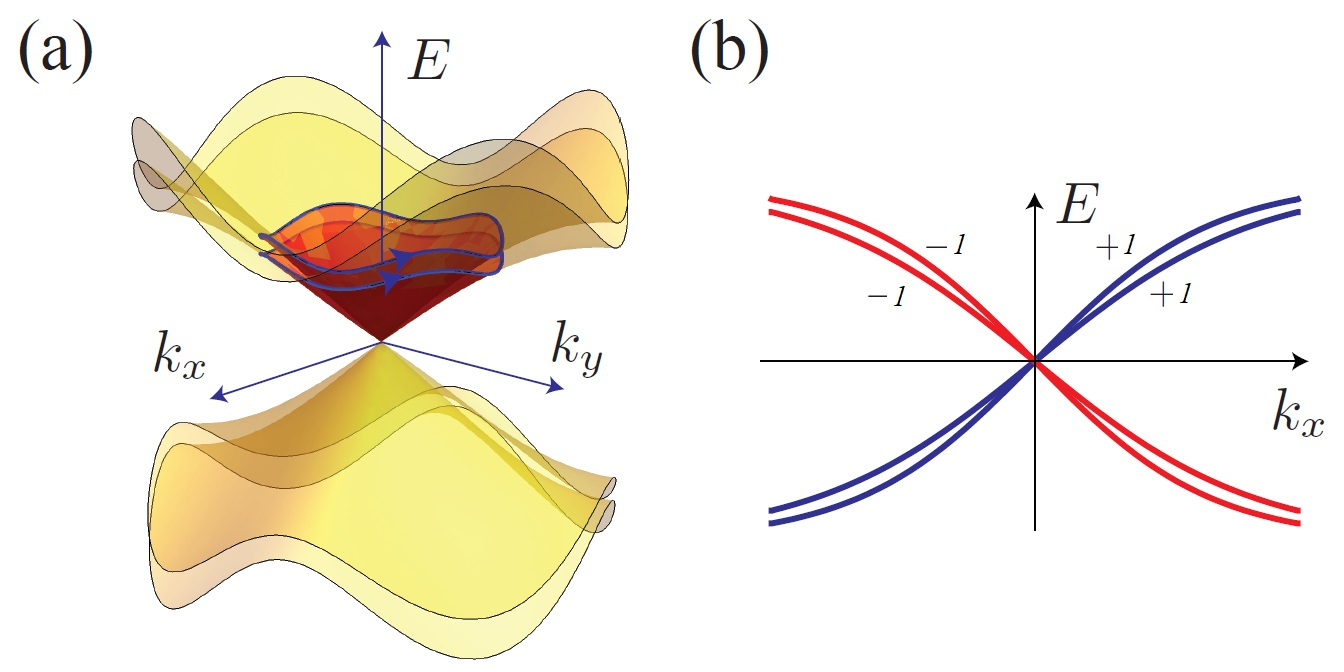
\includegraphics[width=0.9\textwidth]{MajoranaCone.jpg}
	\caption[The energy spectrum of Dirac nodal superconductor.]{(a) The energy spectrum of Dirac nodal superconductor along the mirror symmetric plane($k_z=0$). The Dirac nodal superconductor is protected by non-trivial mirror winding (blue curve) around the nodal point. (b) The same dispersion as (a) but now labeled with the mirror-glide eigenvalue(red and blue), $g$. Each mirror branch now connects at higher momentum, and they switch each other.}\label{fig:MajoranaCone}
\end{figure}

As the nodal points in the $3$D Dirac topological superconductor are topologically protected, we now define and evaluate a topological mirror-glide winding invariant. Since both the time-reversal and particle-hole operators commute with the mirror-glide matrix $G$, so does the chiral operator, which is the product $S=-iT\Xi=\tau_y$. Let ${\bf v}_{sg}^1$ and ${\bf v}_{sg}^2$ be two orthonormal simultaneous eigenvectors of $S$ and $G$ with eigenvalues $s=\pm1$ and $g=\pm1$ respectively. Then, we can define the projection operator, $P_{sg}^\dagger=({\bf v}_{sg}^1,{\bf v}_{sg}^2)^\dagger$, that maps onto the two-dimensional fixed eigenvalue subspace. Since the BdG Hamiltonian $H_{\mathrm{SC-Dirac}}$ in Eq. \eqref{DiracSC} commutes with $G$ on the $k_x-k_y$ plane and anticommutes with $S$, it can be summarized by the two $2\times2$ matrices \begin{align}h^{(+)}({\bf k}_\|)&=P_{-+}^\dagger H_{\mathrm{SC-Dirac}}({\bf k}_\|)P_{++},\nonumber\\h^{(-)}({\bf k}_\|)&=P_{--}^\dagger H_{\mathrm{SC-Dirac}}({\bf k}_\|)P_{+-}\end{align} associated with the two distinct mirror sectors, where ${\bf k}_\|$ is the in-plane momentum. As the Hamiltonian is nodal only at the $\Gamma$ point, $h^{(\pm)}({\bf k}_\|)$ is non-singular as long as ${\bf k}_\|\neq0$. Therefore, the winding number of each sector is defined to be the integral \begin{align}N^{(\pm)}=\frac{1}{2\pi i}\oint_{\mathcal{C}}\mathrm{Tr}\left[h^{(\pm)}({\bf k}_\|)^{-1}\nabla_{{\bf k}_\|}h^{(\pm)}({\bf k}_\|)\right]\cdot d{\bf k}_\| \,, \label{Mwinding}\end{align} where $\mathcal{C}$ can be taken to be any (anti-clockwise) loop around the origin on the momentum plane. This integral represents the same winding invariant that characterizes the surface Majorana cone of a time-reversal invariant topological superconductor. This analysis confirms that along the mirror symmetric plane, the gapless Majorana fermions corresponding to each mirror-glide sector are equivalent to those on the surface of a time-reversal invariant topological superconductor with index $N=\pm2$\cite{Ryu2008}.  For the Dirac nodal superconductor in Eq. \eqref{DiracSC}, these winding numbers are $N^{(+)}=-N^{(-)}=2$. The two sectors must have opposite invariants as the overall system is anomalous-free. In general, we define the mirror winding number to be $N=N^{(+)}=-N^{(-)}$. Since the winding number in Eq. \eqref{Mwinding} must be an integer and cannot change continuously, a nodal superconductor with non-trivial mirror winding is topological protected as long as the symmetries are preserved. It is important to note that the glide mirror symmetry in our model squares to $1$, which is different from the conventional mirror symmetry in a spinful system. If $G^2=-1$ (up to a translation), the eigenvalues of $G$ are $\pm i$. In this case, we can define the mirror wining number of $G=+i$ and $G=-i$ sectors respectively. However $T$ flips between the two sectors of $G$. Therefore the winding number of the $G=+i$ branch must be equal to that of the $G=-i$ branch. So the net winding number is now non-zero. As a result, the Dirac nodal superconductor must be anomalous, and as such it can only appear at the boundary of a 4D bulk.



We now consider the presence of chiral Dirac vortices in the 3D Dirac nodal superconductor that break both the time-reversal and mirror-glide symmetries. Each of these vortices host a single chiral (complex) Dirac fermion. They constitute a three dimensional array of coupled vortices that restores the symmetries in low-energy long length-scale. The BdG defect Hamiltonian of the vortex array consists of the nodal Hamiltonian in Eq. \eqref{DiracSC} together with the symmetry breaking terms
\begin{align}
H_{\mathrm{SC-Dirac}}({\bf k},{\bf r})&=\hbar v{\bf k}\cdot\vec\sigma\mu_z\tau_z\nonumber\\&\;\;\;\;+\Delta_1({\bf r})\tau_x+\Delta_2({\bf r})\mu_z\tau_y.
\label{varray}
\end{align} $\Delta({\bf r})=\Delta_1({\bf r})+i\Delta_2({\bf r})$ is the order parameter that acts independently on the two Weyl species labeled by $\mu_z=\pm1$ and slowly modulates in space. When $\Delta({\bf r})=|\Delta|e^{i\varphi({\bf r})}$ forms a vortex configuration in that its phase $\varphi$ spatially winds by $2\pi$ around the defect line. Each Weyl sector in the Hamiltonian supports a chiral (real) Majorana channel along the vortex lines. These are quasi-one-dimensional structures that host gapless Majorana fermion excitations. The Majorana fermions are localized on the vortex line and they are chiral in the sense that they can only propagate along a single direction. The superconducting pairing potentials in Eq. \eqref{varray} are chosen so that the phases of the order parameter are conjugated between the two Weyl species. Together with the fact that the two Weyl species have the opposite Chern numbers, the pair of chiral Majorana channels supported by them are propagating in the same direction and are protected. For instance, electron tunnelings between the pair are forward scattering processes that only renormalize the velocity and cannot introduce a mass. The pair of co-propagating Majorana fermions can be combined into a single chiral Dirac fermion $d\sim\gamma_++i\gamma_-$.


\begin{figure}[htbp]
	\centering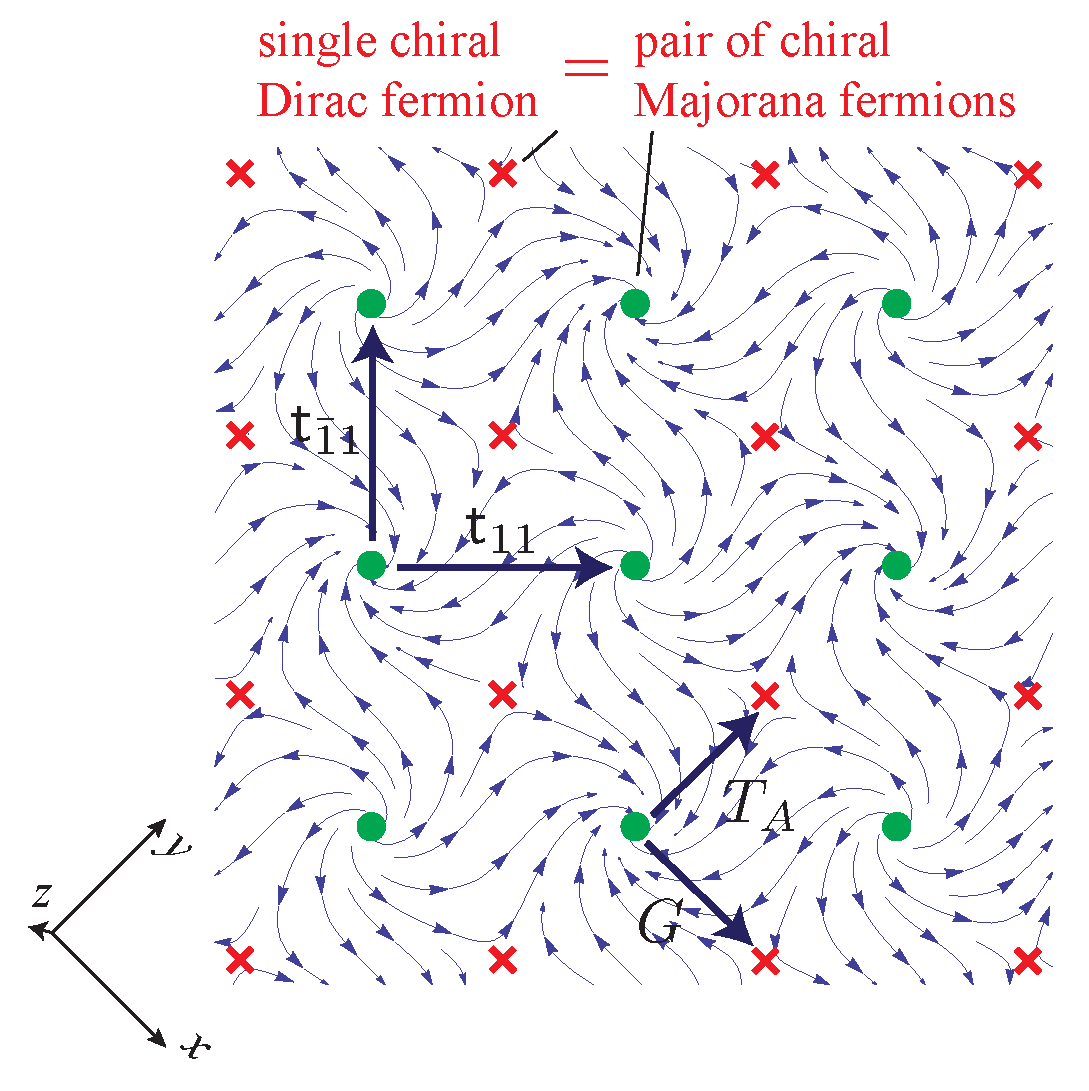
\includegraphics[width=0.6\textwidth]{chiralDiracvortices}
	\caption[Arrays of chiral Dirac channels that we use as a basis for constructing the 3D nodal Dirac superconductor in this work.]{Arrays of chiral Dirac channels that we use as a basis for constructing the 3D nodal Dirac superconductor in this work. The vortex array is symmetric under antiferromagnetic time-reversal $T_A$ and mirror-glide $G$. The vector field represents the pairing phase of the host superconducting state. Each {\color{green}$\bullet$} and {\color{red}$\times$} represents a neutral Dirac fermion channel parallel and opposite to the $z$-axis.}\label{fig:chiralDiracvortices}
\end{figure}

A periodic array of chiral Dirac vortices can be realized by the pairing configuration
\begin{align}
\Delta({\bf r})=\Delta_0\frac{\mathrm{sd}(x+iy)}{|\mathrm{sd}(x+iy)| /,,}
\end{align} where $\mathrm{sd}$ is the (rescaled) Jacobian elliptic function~\cite{ReinhardtWalker10} with simple zeros and poles at $p+iq$ and $(p+1/2)+i(q+1/2)$ respectively, $p,q$ are integers. Fig. \ref{fig:chiralDiracvortices} shows the checker board lattice, and ${\bf e}_x$ and ${\bf e}_y$ form a lattice translational vector. We find that the phase $\varphi$ of $\Delta=|\Delta|e^{i\varphi}$ winds by $2\pi$ around each integral lattice point and $-2\pi$ around a half-integral one. The vortex lines are directed along $z$ and form a checkerboard lattice along $x$ and $y$. Nearest neighbor vortices host counter-propagating Dirac modes so that a right-moving chiral Dirac channel appears at $(p,q)$ and a left-moving one appears at $(p+1/2,q+1/2)$.
We choose $\Delta_0=|\Delta_0|e^{i\pi/4}$ so that the pairing order parameter transforms under
\begin{gather}
\Delta({\bf r})=-\Delta({\bf r}+{\bf e}_x)=-\Delta({\bf r}+{\bf e}_y),\nonumber\\\Delta\left({\bf r}+\frac{{\bf e}_x\pm{\bf e}_y}{2}\right)=\pm\Delta({\bf r})^\ast.
\end{gather}
Although the pairing order parameter has periods $(1,1)$ and $(1,-1)$, the Bogoliubov-de Gennes (BdG) Hamiltonian in Eq. \eqref{varray} has finer artificial lattice translation symmetries $\mathsf{t}_x,\mathsf{t}_y$. The Hamiltonian symmetric under $\mathsf{t}_x,\mathsf{t}_y$ satisfies,
\begin{align}
\mu_y\tau_yH_{\mathrm{SC-Dirac}}({\bf k},{\bf r})\mu_y\tau_y&=H_{\mathrm{SC-Dirac}}({\bf k},{\bf r}+{\bf e}_x)\nonumber\\&=H_{\mathrm{SC-Dirac}}({\bf k},{\bf r}+{\bf e}_y).
\label{latticetranslationH}
\end{align}
The Hamiltonian is symmetric under particle-hole operator, $\Xi$, and it follows the condition given as,
\begin{align}s_y\tau_yH_{\mathrm{SC-Dirac}}({\bf k},{\bf r})^\ast s_y\tau_y=-H_{\mathrm{SC-Dirac}}(-{\bf k},{\bf r}).\end{align}
Furthermore, our particular vortex geometry possesses an antiferromagnetic time-reversal $T_A$, which is a combination of the time reversal $T$ and a half-translation by $({\bf e}_x+{\bf e}_y)/2$.
\begin{align}s_yH_{\mathrm{SC-Dirac}}({\bf k},{\bf r})^\ast s_y=H_{\mathrm{SC-Dirac}}\left(-{\bf k},{\bf r}+\frac{{\bf e}_x+{\bf e}_y}{2}\right).\label{TAH}
\end{align}
The vortex array also possesses the mirror-glide symmetry $G$, which combines mirror along the $x-y$ plane with a half-translation by $({\bf e}_x-{\bf e}_y)/2$,
\begin{align}&s_z\tau_yH_{\mathrm{SC-Dirac}}({\bf k},{\bf r})s_z\tau_y\nonumber\\&\;\;\;=H_{\mathrm{SC-Dirac}}\left(M{\bf k},M{\bf r}+\frac{{\bf e}_x-{\bf e}_y}{2}\right),\label{GH}\end{align}
where we define the mirror symmetry operator as, $M:(x,y,z)\to(x,y,-z)$.



We now focus on the low-energy chiral Dirac modes in the vortex array. Let $d_{x,y,k}$ be the chiral Dirac mode at $(x,y)$ with momentum $k_z=k$. When $x\equiv y$ modulo 2, $d_{x,y,k}=R_{x,y,k}$ propagates in the $+z$ direction, and when $x\equiv y+1$ modulo 2, $d_{x,y,k}=L_{x,y,k}$ propagates in the $-z$ direction. $R$ and $L$ are respectively represented by crosses and dots in Fig.~\ref{fig:chiralDiracvortices}. Each is a combination of a pair of chiral Majorana modes that are originated from the two opposite Weyl species. $R\sim\gamma_R^{(+)}+i\gamma_R^{(-)}$, where the sign refers to chirality of the original Weyl species $\mu_z=\pm1$, and similar definitions extend to the $-z$ directed modes as $L\sim\gamma_L^{(+)}+i\gamma_L^{(-)}$. Due to the presence of the underlying symmetries in the system, the Dirac fermions transform according to \begin{gather}\mathsf{t}_{11}R_{x,y,k}\mathsf{t}_{11}^{-1}=R_{x+1,y+1,k},\quad\mathsf{t}_{\bar{1}1}R_{x,y,k}\mathsf{t}_{\bar{1}1}^{-1}=R_{x-1,y+1,k},\nonumber\\\mathsf{t}_{11}L_{x,y,k}\mathsf{t}_{11}^{-1}=L_{x+1,y+1,k},\quad\mathsf{t}_{\bar{1}1}L_{x,y,k}\mathsf{t}_{\bar{1}1}^{-1}=L_{x-1,y+1,k},\nonumber\\T_AR_{x,y,k}T_A^{-1}=L_{x,y+1,-k},\quad T_AL_{x,y,k}T_A^{-1}=-R_{x,y+1,-k},\nonumber\\GR_{x,y,k}G^{-1}=iL_{x+1,y,-k}^\dagger,\quad GL_{x,y,k}G^{-1}=iR_{x+1,y,-k}^\dagger,\label{CWsymmetries}\end{gather} They form a representation that is consistent with the symmetry algebra $[\mathcal{O},\mathcal{O}']=0$ for $\mathcal{O},\mathcal{O}'=T_A,G,\mathsf{t}_{11},\mathsf{t}_{\bar{1}1}$, $T_A^2=(-1)^F\mathsf{t}_{11}\mathsf{t}_{\bar{1}1}$ and $G^2=\mathsf{t}_{11}\mathsf{t}_{\bar{1}1}^{-1}$, where $(-1)^F$ is the fermion parity operator and $T_A$ is antiunitary.

\begin{figure}[htbp]
	\centering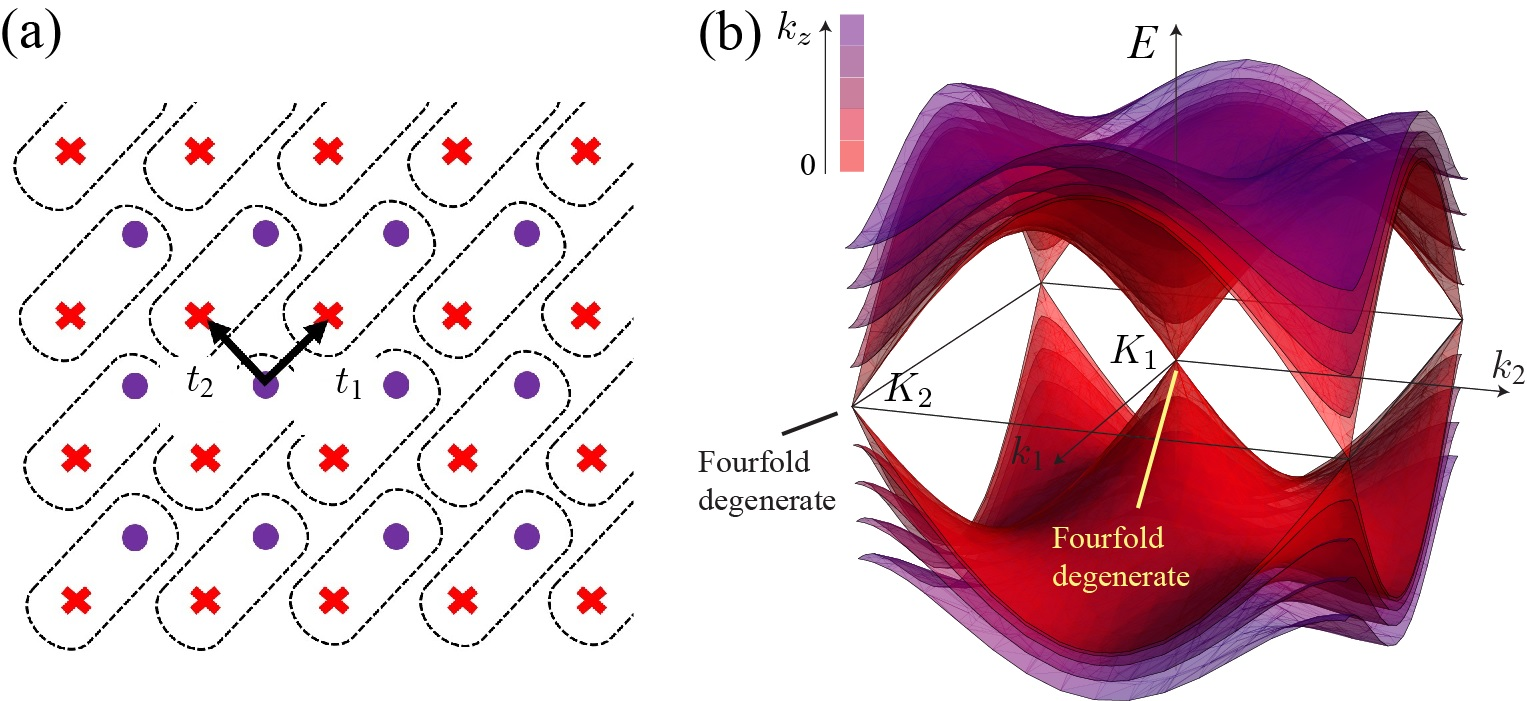
\includegraphics[width=0.96\textwidth]{BdGspectrum.jpg}
	\caption[Schematic figure of the coupled wire model and the energy spectrum of the BdG model.]{(a) Schematic figure of the coupled wire model that we use in this work. Each unit cell (as denoted by the dashed black boxes) consists of a pair of counter-propagating Dirac modes, labeled by red cross and purple dot. The black arrows indicate tunneling amplitudes $t_1$ and $t_2$ between different Dirac modes. (b) Energy spectrum of the BdG model \eqref{Eq:BdG} of the coupled wire model. We find the two nodal points, $K_1$ and $K_2$, showing the massless Dirac dispersions.}\label{fig:3Darray}
\end{figure}


Integrating out the gapped bulk modes far away from the Fermi energy, the low-energy effective Hamiltonian can be written as \begin{gather}H_{||}(k)=\hbar v_fk\sum_{x\equiv y}\left(R_{x,y,k}^\dagger R_{x,y,k}-L_{x+1,y,k}^\dagger L_{x+1,y,k}\right) \,, \label{Hparallel}\end{gather} where $v_f$ is the Fermi velocity of the Dirac fermions. When the wires are close to each other, there are finite hybridizations between the Dirac modes. We add interwire fermion quasiparticle tunneling terms in the $[110]$ and $[1\bar{1}0]$ directions. The presence of these terms in our model introduces an energy dispersion in the perpendicular directions. The symmetry-preserving interwire hopping terms can be written as,
\begin{gather}
H_{\perp,1}(k)=\sum_{x\equiv y}it_1\left(L^\dagger_{x,y+1,k}-L^\dagger_{x,y-1,k}\right)R_{x,y,k}+h.c.,
\\
H_{\perp,2}(k)=\sum_{x\equiv y}t_2\left(L^\dagger_{x-1,y,k}-L^\dagger_{x+1,y,k}\right)R_{x,y,k}+h.c. \,,
\end{gather}
where the tunneling strengths $t_1$ and $t_2$ are real numbers. In Fig.~\ref{fig:3Darray}(a), we schematically represent the physical picture of the counter-propagating modes with the corresponding interwire hopping terms, $t_1$ and $t_2$ that account for the interwire tunneling resulting from the spatial proximity between Dirac wires. By collecting the interwire hopping terms in both directions, the Hamiltonian of the coupled wire model is
\begin{align}\mathcal{H}&=\sum_{k}H_{||}(k)+H_{\perp,1}(k)+H_{\perp,2}(k).\label{Eq:WeylHam}\end{align} The model is symmetric under lattice translations, antiferromagnetic time-reversal, and mirror-glide symmetries as: \begin{align}\mathsf{t}_{11,\bar{1}1}^{-1}\mathcal{H}\mathsf{t}_{11,\bar{1}1}=T_A^{-1}\mathcal{H}T_A=G^{-1}\mathcal{H}G=\mathcal{H}.\end{align} After Fourier transform, the single-body system can be captured by the BdG Hamiltonian in the momentum space, \begin{align}\mathcal{H}&=\frac{1}{2}\sum_{k_1,k_2,k_z}\boldsymbol\xi_{\bf k}^\dagger H_{BdG}({\bf k})\boldsymbol\xi_{\bf k},\nonumber\\
H_{BdG}({\bf k})&=\begin{pmatrix}H({\bf k})&0\\0&-\sigma_yH(-{\bf k})^T\sigma_y\end{pmatrix},\label{Eq:BdG}\\
H({\bf k})&=\begin{pmatrix}
\hbar v_fk_z & q(k_1,k_2) \\
q(k_1,k_2)^\ast & -\hbar v_fk_z \\
\end{pmatrix},\nonumber
\end{align}
where $\boldsymbol\xi_{\bf k}=(R_{\bf k},L_{\bf k},L_{-{\bf k}}^\dagger,-R_{-{\bf k}}^\dagger)^T$ is the Nambu vector, $H({\bf k})$ is the Hamiltonian defined in Eq.~\eqref{Eq:WeylHam}, and $q(k_1,k_2)=it_1(1-e^{-i(k_1+k_2)})+t_2(e^{-ik_1}-e^{-ik_2})$. Here, $k_1$ is directed along the $(11)$-direction and $k_2$ is along the $(\bar{1}1)$-direction. From this point forward, we set $\hbar v_f=t_1=t_2=1$ (in units of $eV$) for simplicity but without loss of generality. In analyzing our model, we find that $q(0,0)=q(\pi,\pi)$ vanishes, therefore the Hamiltonian in Eq.~\eqref{Eq:WeylHam} possesses the two Weyl nodes at $K_1=(0,0,0)$ and $K_2=(\pi,\pi,0)$. We may write the low-energy expansion of the Hamiltonian near each of the Weyl points as,
\begin{gather}
H(K_{1,2}+{\bf k})\approx \nonumber
\\ \left(\begin{matrix}
k_z & -t_1(k_1+k_2) \mp it_2(k_1-k_2) \\
-t_1(k_1+k_2) \pm it_2(k_1-k_2) & -k_z \\
\end{matrix}\right)\label{Eq:weylexpand}
\end{gather}
for small $|k| \ll 1$. From Eq.~\eqref{Eq:weylexpand}, we find that the Hamiltonian is comprised of a pair of Weyl fermions with opposite chiralities and we plot the resulting energy spectra in the low-energy limit in Fig.~\ref{fig:3Darray}(b).


Unlike the Weyl semimetals that has the charge conservation, our model is based on a charge breaking superconducting medium. The Weyl fermions here are not protected by the Chern number. This is because the BdG Hamiltonian in Eq. \eqref{Eq:BdG} has two opposing diagonal blocks. At each of the corresponding gap closing points $K_{1,2}$, there are two coinciding massless nodes in the BdG description and they have opposite Chern numbers. In fact, as the nodal points are inversion symmetric, where $K_{1,2}=-K_{1,2}$ (modulo reciprocal vectors), the particle-hole symmetry forbids a non-vanishing net Chern number. As a result, the Weyl fermions, in the absence of the symmetries, can acquire finite masses by the addition of off-diagonal terms in the BdG Hamiltonian of Eq. \eqref{Eq:BdG}. However, these terms are absent in our model because of the particle-hole, antiferromagnetic, and mirror-glide symmetries: \begin{align}\Xi H_{BdG}({\bf k})^\ast&=-H_{BdG}(-{\bf k})\Xi,\nonumber\\T_A({\bf k})H_{BdG}({\bf k})^\ast&=H_{BdG}(-{\bf k})T_A({\bf k}),\\G({\bf k})H_{BdG}({\bf k})&=H_{BdG}(M{\bf k})G({\bf k}),\nonumber\end{align} where the Nambu vector transforms according to \begin{align}\boldsymbol\xi_{\bf k}^\dagger&=\Xi\boldsymbol\xi_{-{\bf k}},\nonumber\\T_A\boldsymbol\xi_{\bf k}T_A^{-1}&=T_A({\bf k})\boldsymbol\xi_{-{\bf k}},\\G\boldsymbol\xi_{\bf k}G^{-1}&=G({\bf k})\boldsymbol\xi_{M{\bf k}},\nonumber\end{align} where $M$ is defined as $M:(k_1,k_2,k_z)\to(k_1,k_2,-k_z)$, and the symmetry matrices are given by \begin{gather}\Xi=\sigma_y\tau_y\nonumber\\T_A({\bf k})=\left(\begin{smallmatrix}0&1&0&0\\-e^{-i(k_1+k_2)}&0&0&0&\\0&0&0&e^{-i(k_1+k_2)}\\0&0&-1&0\end{smallmatrix}\right)\\G({\bf k})=\left(\begin{smallmatrix}0&0&ie^{-ik_2}&0\\0&0&0&-ie^{ik_1}\\-ie^{ik_1}&0&0&0\\0&ie^{-ik_2}&0&0\end{smallmatrix}\right).\nonumber\end{gather} The gapless nodes at $K_{1,2}$ are protected by the non-trivial mirror winding number $N(K_{1,2})=N^{(+)}(K_{1,2})=1$ defined in Eq. \eqref{Mwinding}. The winding numbers are equal at the two nodal momenta and, therefore, they add up to the net non-trivial mirror winding number $N=N(K_1)+N(K_2)=2$, which is identical to that of the homogeneous superconducting Dirac parent state in Eq. \eqref{DiracSC}. In other words, the coupled wire model recovers the Dirac nodal superconductor in low-energy limit. \begin{align}\begin{diagram}\stackrel{\mbox{Dirac nodal}}{\mbox{superconductor}}&\pile{\rTo^{\mbox{\small chiral vortices}}\\\lTo_{\mbox{\small coupled wire model}}}&\mbox{chiral Dirac strings}\end{diagram}\end{align}


We conclude this section by commenting the stability of Dirac nodal superconductors in the single-body setting. We first notice that the continuum model Hamiltonian, $H_{\mathrm{SC-Dirac}}$ in Eq. \eqref{DiracSC}, can be broken down into two pieces according to the Weyl species $\mu_z$. Each piece corresponds to a {\em Weyl nodal superconductor} \begin{align}H_{\mathrm{SC-Dirac}}=\pm\hbar v{\bf k}\cdot\vec{s}\tau_z,\label{WeylSC}\end{align} which is protected by time-reversal and glide symmetries and has the non-trivial mirror winding number $N=N^{(+)}=-N^{(-)}=1$. We are referring to Eq. \eqref{WeylSC} as a ``Weyl" nodal superconductor because the BdG nodal point is fourfold degenerate, which is equivalent to two distinct physical fermion degrees of freedom when the artificial Nambu doubling is taken away. This should not be confused with a Weyl (semi)metal for the following reasons: First, the nodal point is at $\bf k=0$, which is a time-reversal invariant momentum, and the particle-hole symmetry requires the Chern number of the BdG bands around the nodal point to vanish. Second, the BdG Hamiltonian cannot simply be a Nambu doubling of a Weyl (semi)metal because there is no regularizable charge preserving model with only one Weyl species.

\begin{figure}[htbp]
	\centering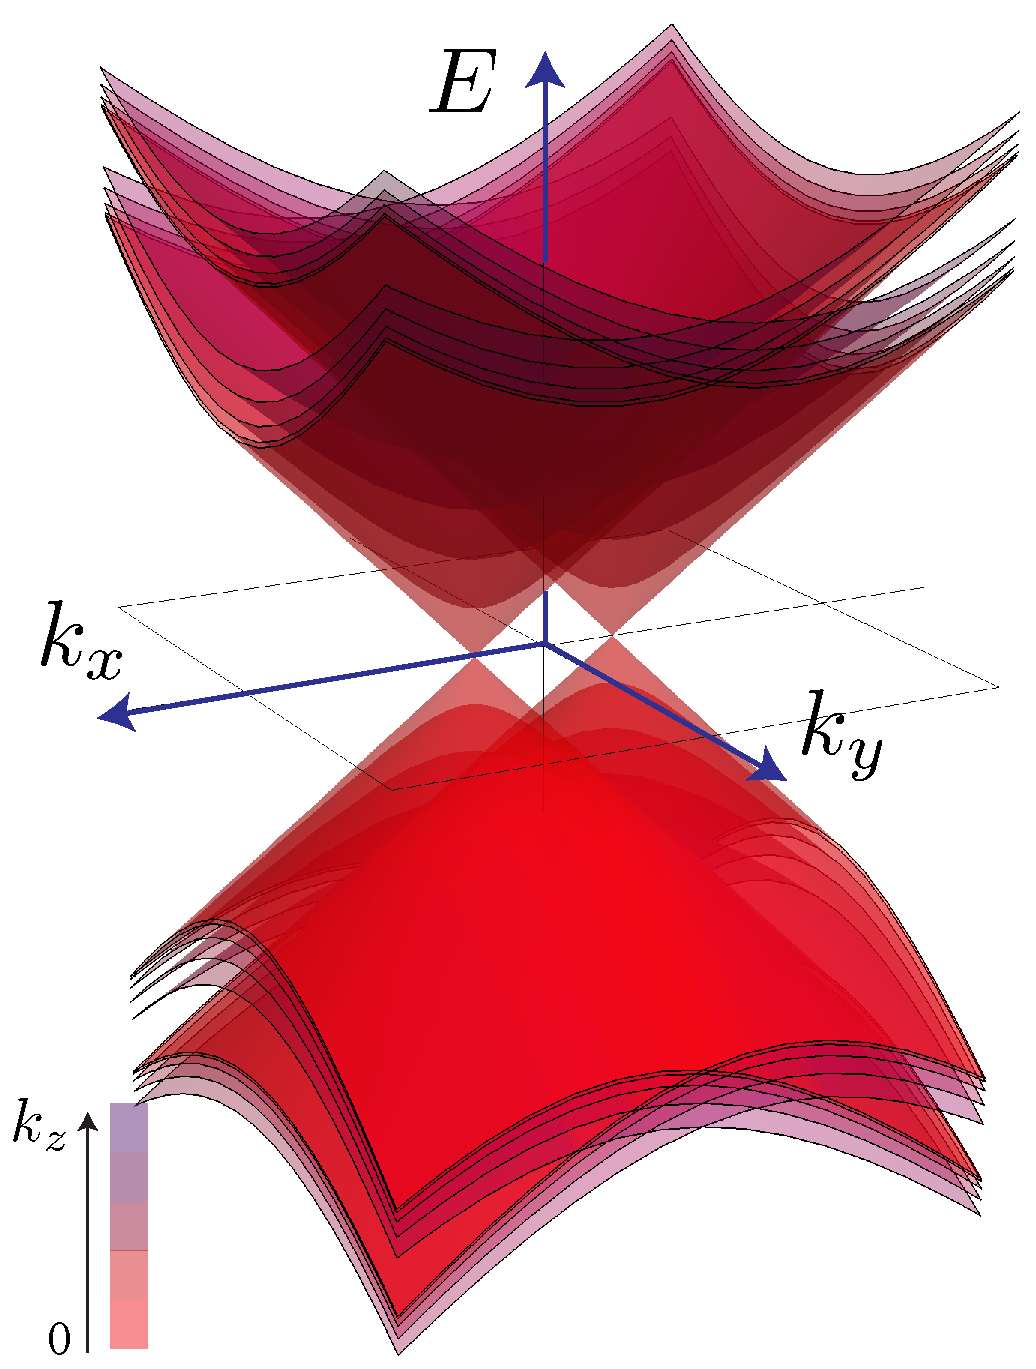
\includegraphics[width=0.3\textwidth]{Hcontsplit}
	\caption[The splitting of the two nodal Weyl points of a Dirac nodal superconductor.]{The splitting of the two nodal Weyl points of a Dirac nodal superconductor by the symmetry preserving perturbation in Eq. \eqref{DiracSCsplit}.}\label{fig:Hcontsplit}
\end{figure}

A Weyl nodal superconductor is stable to all perturbations because there is no symmetry preserving gapping potentials and the nodal point is pinned by time-reversal. On the other hand, a Dirac nodal superconductor is only stable up to weak perturbation. While it is true that there is no symmetry preserving potentials that can immediately introduce an excitation energy gap, the two nodal Weyl species can be split in momentum space. For example, the following perturbation introduces the split. \begin{align}H_{\mathrm{SC-Dirac}}=\hbar v{\bf k}\cdot\vec{s}\mu_z\tau_z+us_x\mu_y\tau_x,\label{DiracSCsplit}\end{align} where the two nodal Weyl points split along the $x$-axis (See Fig.~\ref{fig:Hcontsplit}). Each nodal Weyl point is fourfold degenerate. The net Chern number of the BdG bands around each nodal point is still trivial due to the glide symmetry. Instead, it is protected by the mirror winding number $N=1$, which is well defined as long as one stay in one of the two glide eigenspaces. However, if the perturbation is big enough, the two nodal Weyl points can be pushed to the boundary of the Brillouin zone, where the glide eigenvalues switch. The two nodal Weyl points will now have opposite mirror windings and can pair annihilate. A Dirac nodal superconductor is therefore stable against symmetry-preserving perturbations up to $u\lesssim hv/a$, where $a$ is the microscopic length scale of the glide translation.

In a similar way as the continuum model, the coupled wire model in Eq. \eqref{Eq:WeylHam} has two separated Weyl nodes at $K_1$ and $K_2$ (see Fig.~\ref{fig:3Darray}(b)). They are pinned by the (anti-ferromagnetic) time-reversal symmetry and therefore the model is stable to single-body symmetry-preserving perturbations to arbitrary strength. If we dress the model with additional Dirac fermion flavors $d^1,\ldots,d^N$, there will be $N$ nodal Weyl points at each of the two high symmetry momenta $K_1$ and $K_2$. However, similar to the continuous case in Eq. \eqref{DiracSCsplit}, they can now split in pairs. For example, We here illustrate the case when there are $N=2$ fermion flavors. The unperturbed Hamiltonian $\mathcal{H}=\mathcal{H}^{(1)}+\mathcal{H}^{(2)}$ is two decoupled copies of the primitive one, where $\mathcal{H}^{(a)}$ is identical to Eq. \eqref{Eq:WeylHam} by substituting the fermions $R,L$ with $R^a,L^a$. We decompose the Dirac fermions $d=R,L$ into Majorana components $d^a=(\gamma^a+i\delta^a)/\sqrt{2}$ and introduce the symmetry-preserving dimerization \begin{align}\mathcal{H}_{\mathrm{dimer}}=iu\sum_{xy}\gamma^1_{x,y}\gamma^2_{x,y+1}+\delta^1_{x,y}\delta^2_{x,y+1}.\label{Hdimer}\end{align} Then, the full BdG Hamiltonian can be written as,
\begin{align}H_{BdG}^{N=2}({\bf k})=\begin{pmatrix}H_{BdG}({\bf k})&H_{\mathrm{dimer}}({\bf k})\\H_{\mathrm{dimer}}({\bf k})^\dagger&H_{BdG}({\bf k})\end{pmatrix},\label{dimerBdG}
\end{align}
where $H_{BdG}({\bf k})$ is the original $N=1$ Hamiltonian given in Eq. \eqref{Eq:BdG} and the off-diagonal term \begin{align}H_{\mathrm{dimer}}({\bf k})=\frac{iu}{2}\begin{pmatrix}0&1&0&0\\e^{i(k_1+k_2)}&0&0&0\\0&0&0&-e^{i(k_1+k_2)}\\0&0&-1&0\end{pmatrix}\end{align} dimerizes between the two flavors.

\begin{figure}[htbp]
	\centering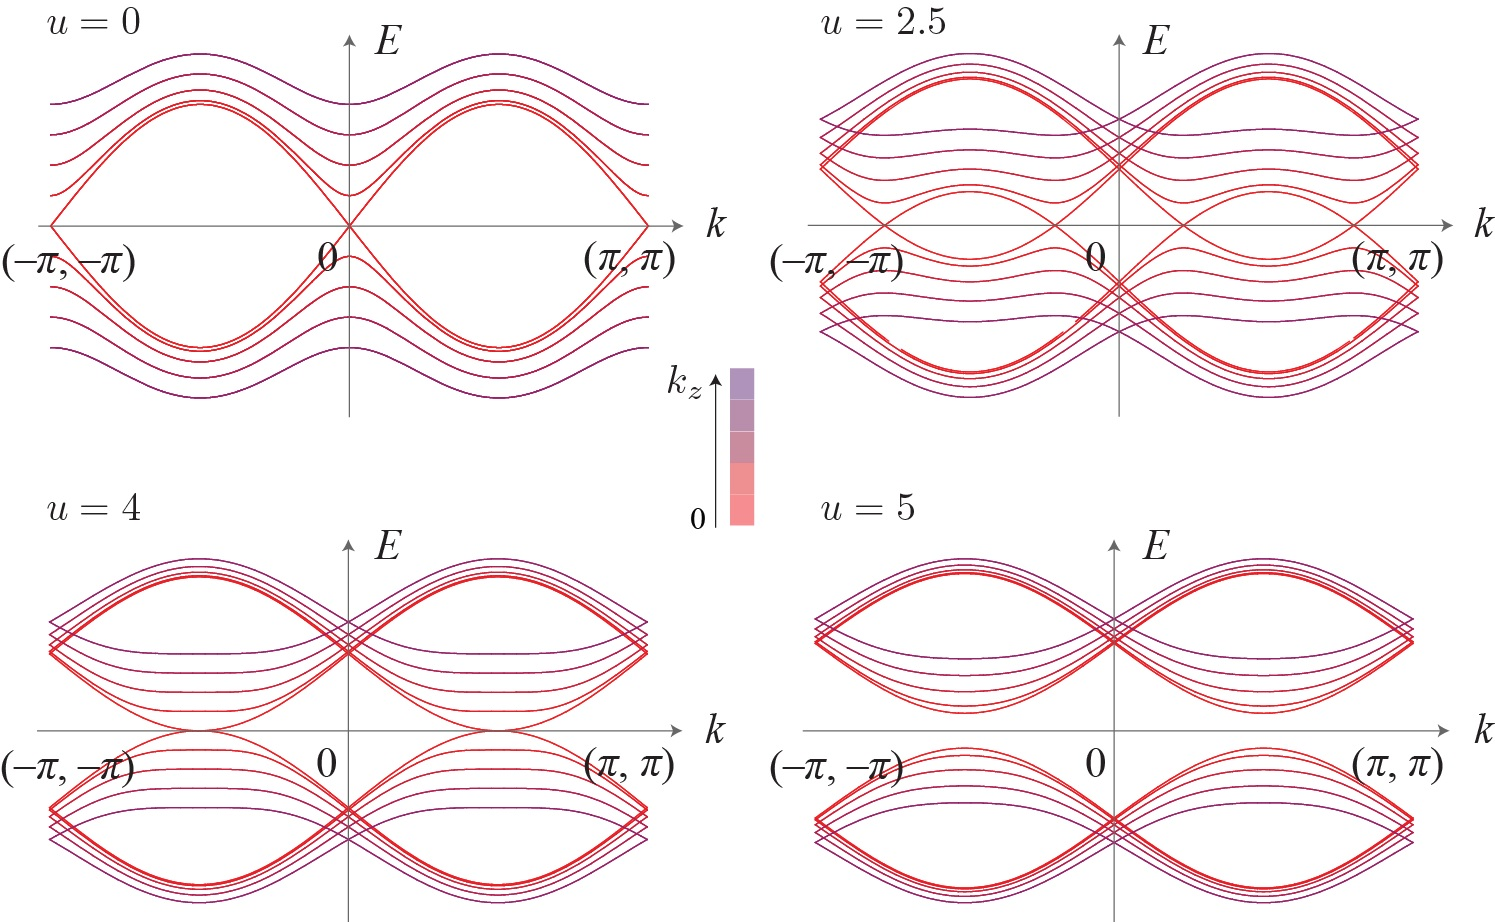
\includegraphics[width=0.9\textwidth]{Z2bands}
	\caption[The BdG energy spectrum of the dimerized system.]{The BdG energy spectrum of the dimerized system in Eq. \eqref{dimerBdG} along the $k_y$-direction (i.e.~$k_1=k_2$) for dimerization strength $u=0,2.5,4,5$ and $t_1=t_2=1$.}\label{fig:Z2bands}
	\centering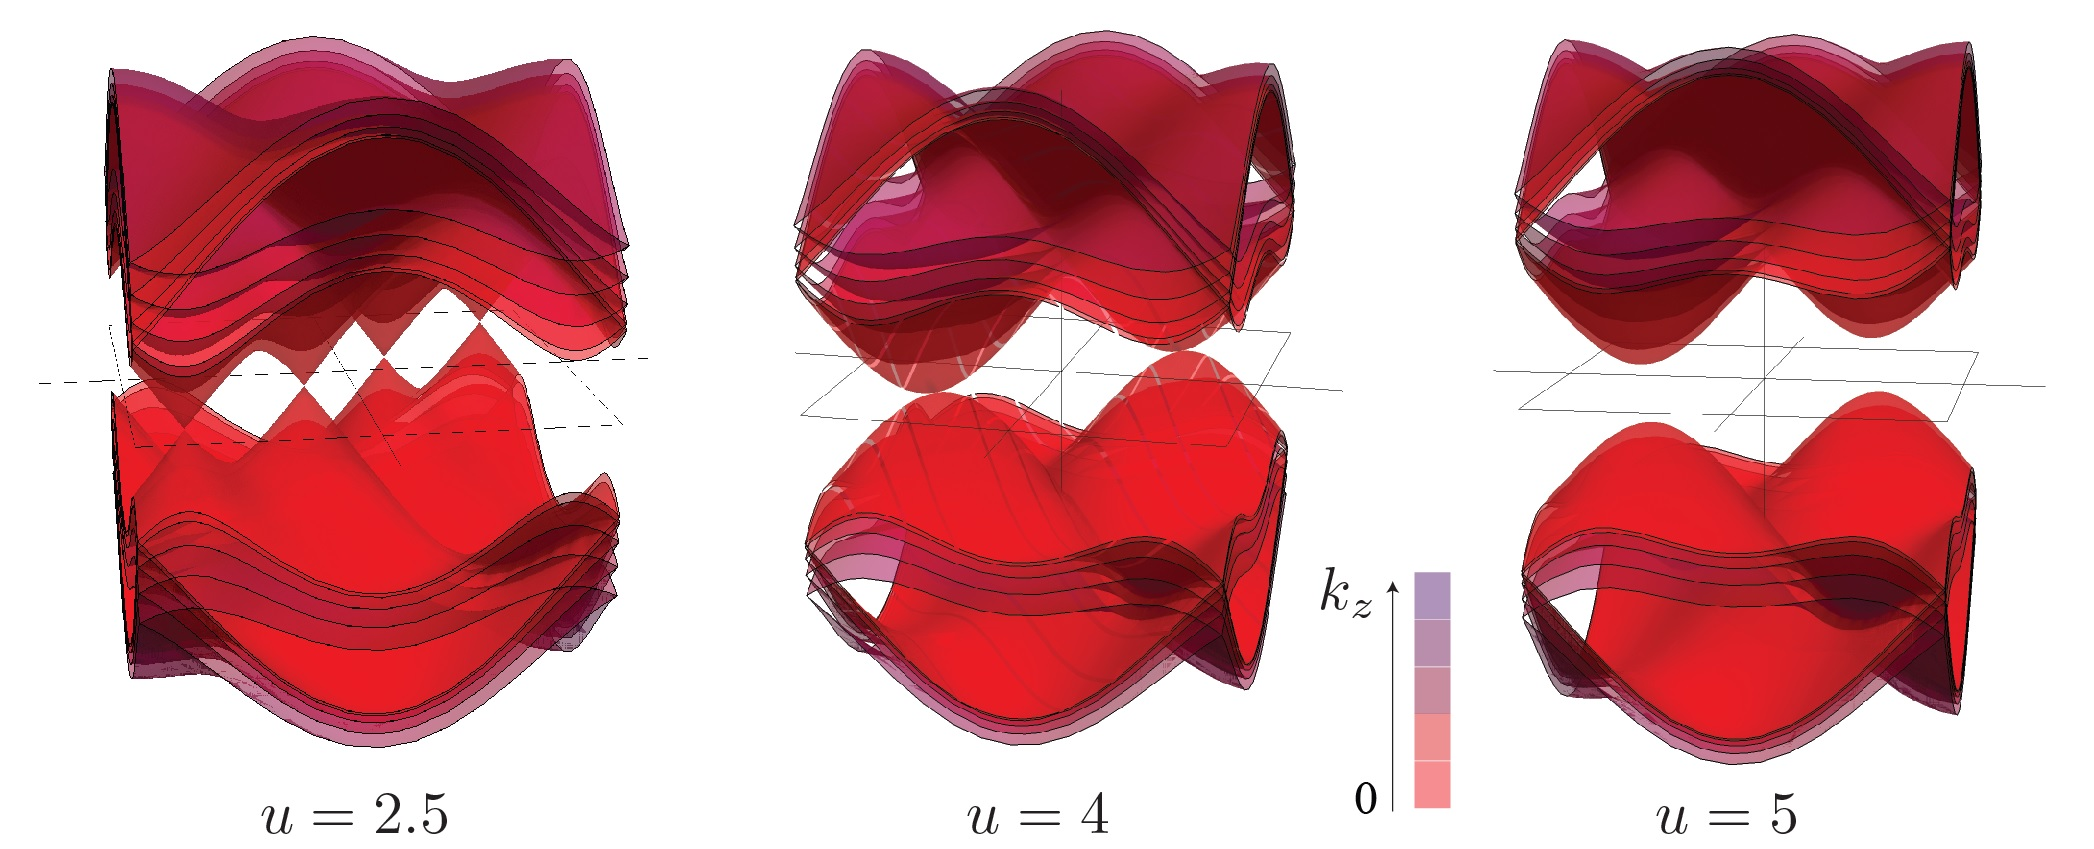
\includegraphics[width=0.96\textwidth]{Z2spectrum}
	\caption[The BdG energy spectrum of the dimerized system over the entire Brillouin zone.]{The BdG energy spectrum of the dimerized system in Eq. \eqref{dimerBdG} over the entire Brillouin zone. As the two nodal Weyl points split in the momentum space, they meet with the other Weyl nodes with the opposite chirality and pair-annihilate each other. This insulator transition confirms the $\mathbb{Z}_2$ classification of our model.}\label{fig:Z2spectrum}
\end{figure}

Figure~\ref{fig:Z2bands} and \ref{fig:Z2spectrum} shows the dimerized energy spectrum. For small $u$, the nodal Weyl points pairwise split along the diagonal $k_y$-axis where $k_1=k_2$. The system remains gapless until the Weyl points originated from opposite momenta $K_{1,2}$ meet. This happens in a system with $u=4t_1=4t_2$ at $(k_1,k_2)=(\pi/2,\pi/2)$ and $(-\pi/2,-\pi/2)$, where Weyl points with opposite mirror windings pair up into quadratic band touching. A finite excitation energy gap opens when $u>4t_1=4t_2$. In the general situation, the coupled wire model with $N$ flavors is stable against any perturbation with strength $u\lesssim t_1,t_2$. If $N$ is odd, there is always an odd number of nodal Weyl points at each of the high symmetry momenta $K_{1,2}$ due to time reversal. They are robust against all single-body perturbations with arbitrary strength. As a result, the nodal coupled wire models are therefore $\mathbb{Z}$ classified for weak perturbation and $\mathbb{Z}_2$ classified for strong ones.
%%



\section{Symmetry preserving many-body gapping interactions}\label{sec:manybody1}
In the previous section, we discussed the Dirac nodal superconductor under the single-body BCS mean-field description. In the low-energy limit, the nodal system was captured by the coupled-wire model in Eq. \eqref{Eq:WeylHam}, which exhibited a pair of massless Weyl fermions located at two time reversal invariant momenta $K_{1,2}$. The massless Weyl fermions are protected by the antiferromagnetic time-reversal $T_A$, mirror-glide $G$ as well as lattice translation $\mathsf{t}_{11},\mathsf{t}_{\bar{1}1}$ symmetries in Eq. \eqref{CWsymmetries}. In general, a nodal point is $\mathbb{Z}$-classified by the mirror-glide winding number in Eq. \eqref{Mwinding}, which counts the number (or net handedness) of massless Weyl fermions. This may be constructed by stacking $N$ copies of the fundamental model in Eq. \eqref{Eq:WeylHam}. This means that each vortex line now hosts, in general, a number of co-propagating chiral Dirac fermions $d^a=R^a$ or $L^a$, where $a$ is the flavor index that runs from 1 to $N$. The massless Weyl fermions are stable against the single-body symmetry preserving perturbations until they pair annihilate. If $N$ is odd, the anitferromagnetic time-reversal symmetry pins at least one massless Weyl node at each of the two high symmetry $K$ points in the Brillouin zone. As the Weyl node cannot move, they are robust even against pair annihilation. Under this non-interacting setup, in this section, we are interested in finding many-body interactions that introduces a finite excitation energy gap, for both even and odd flavor number $N$, while preserving the antiferromagnetic time-reversal, mirror-glide and lattice translation symmetries.

\begin{figure}[htbp]
	\centering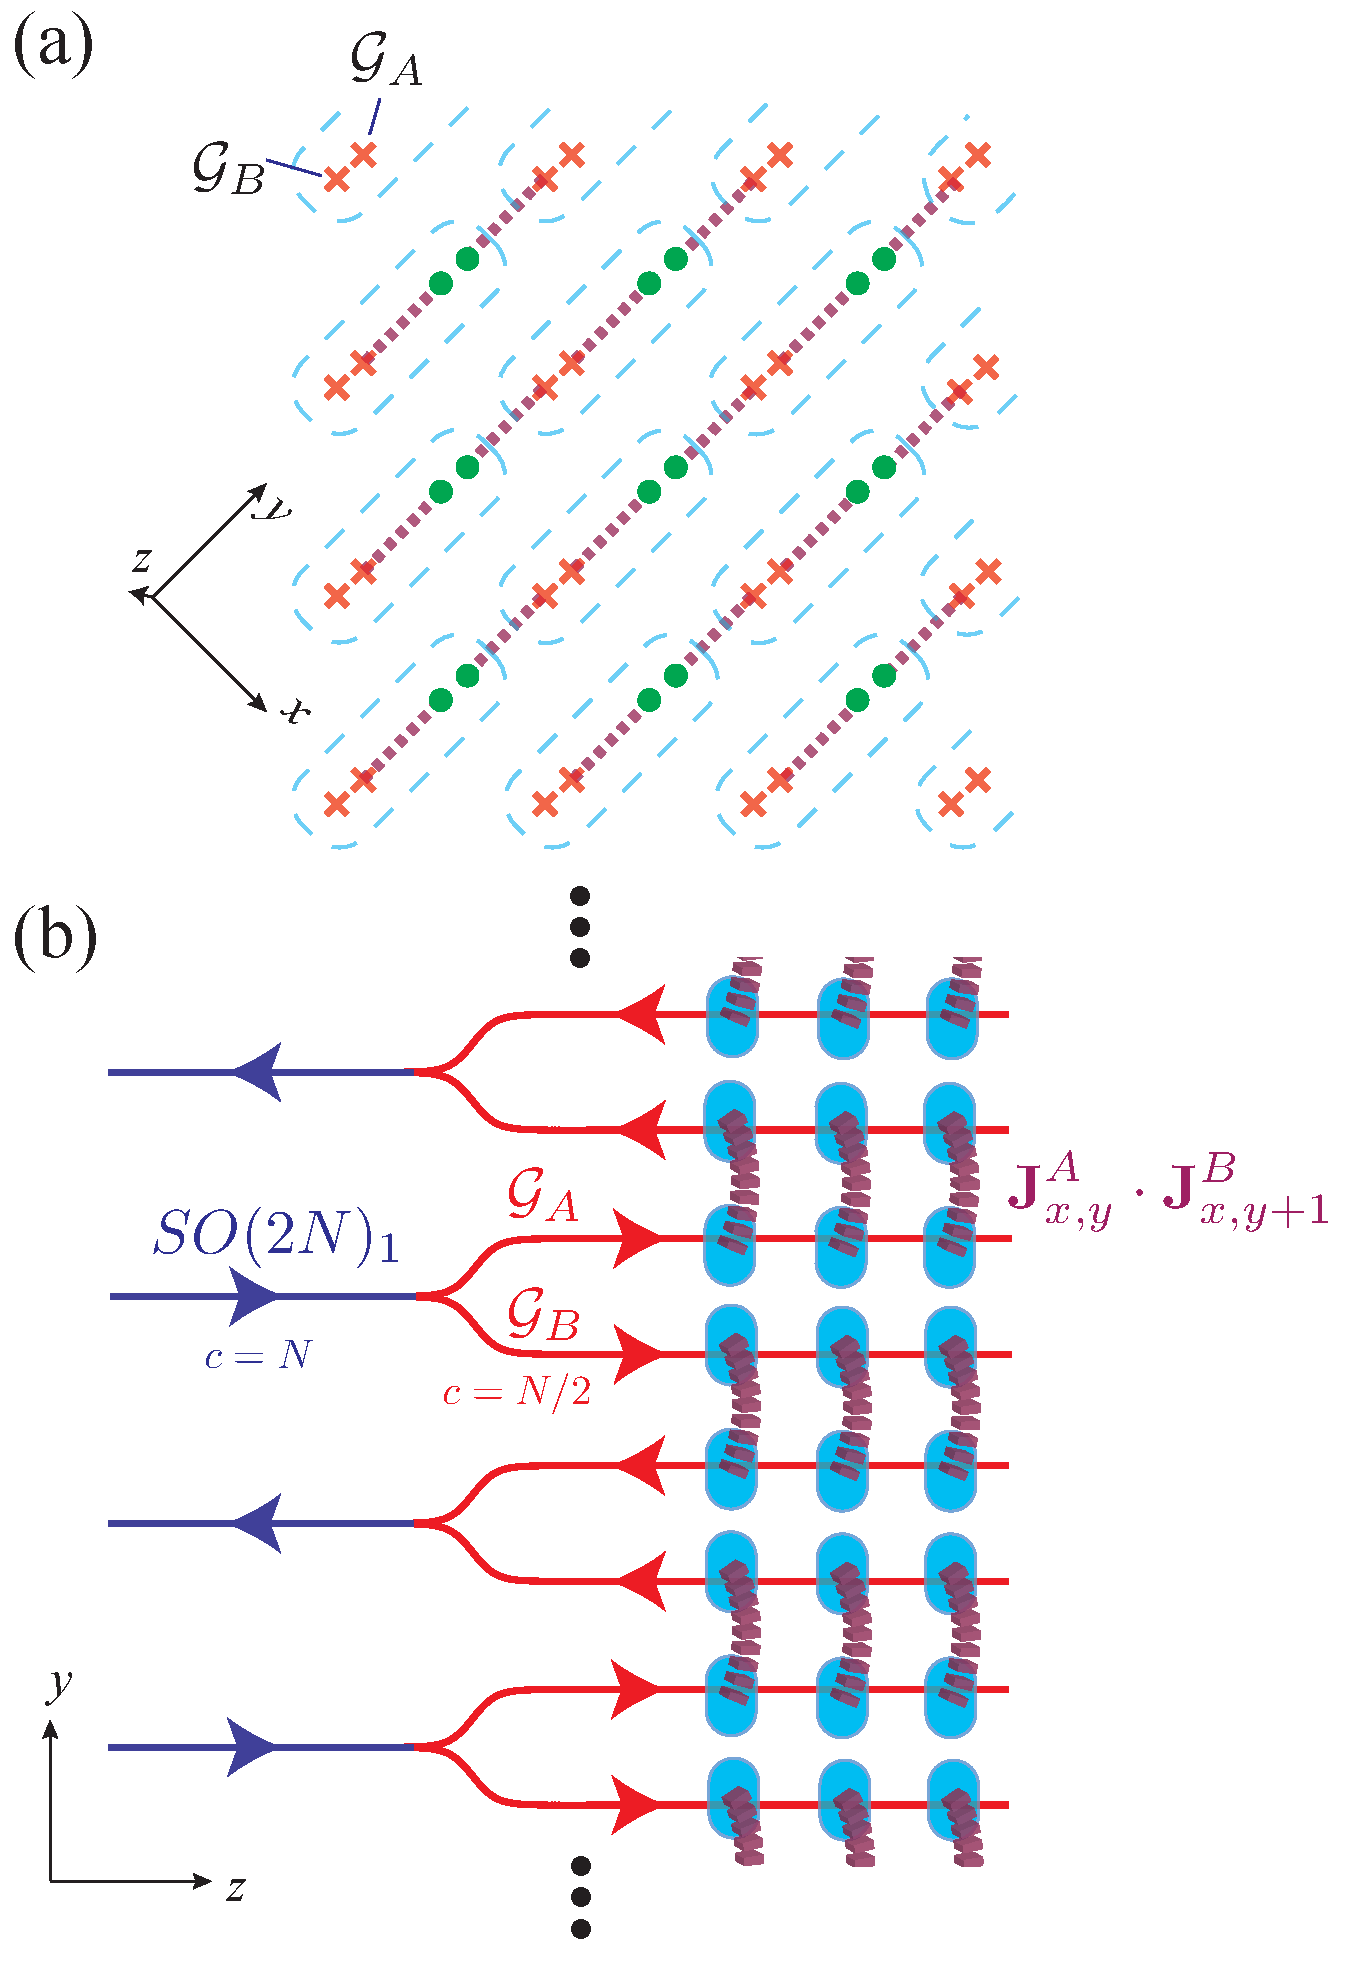
\includegraphics[width=0.8\textwidth]{gappingpotential}
	\caption[Schematic representation of the many-body gapping interactions by interwire current backscatterings.]{Schematic representation of the many-body gapping interactions by interwire current backscatterings. The $N$ Dirac fermions per wire are divided into a pair of $\mathcal{G}$ affine Kac-Moody current algebras. (a) shows the current backscatterings in the 3D system viewed along the wire $z$-direction. (b) shows the current backscatterings on a single $yz$ layer.}\label{fig:gappingpotential}
\end{figure}

Our strategy is based on the coupled-wire construction presented in ref.~\cite{PhysRevB.94.165142}. It relies on a bipartition of degrees of freedom on each vortex line. The degrees of freedom of the $2N$ chiral Majorana fermions $\gamma^a,\delta^a$, which pair into the Dirac fermions $d^a=(\gamma^a+i\delta^a)/\sqrt{2}$ for $a=1,\ldots,N$, are summarized by the $SO(2N)$ Kac-Moody current algebra at level 1 (also referred to as affine Lie algebra or Wess-Zumino-Witten theory). The strategy is to decompose the current algebra into a pair of identical and decoupled components \begin{align}SO(2N)_1\sim\mathcal{G}_A\times\mathcal{G}_B,\label{ABdecomposition}\end{align} where $\mathcal{G}_{A,B}$ are also affine Kac-Moody algebras and they act on decoupled Hilbert spaces $\mathcal{H}_{A,B}$. The decomposition in Eq. \eqref{ABdecomposition} is also known as conformal embedding in the conformal field theory context~\cite{bigyellowbook}. The current operators ${\bf J}^{A,B}$ in $\mathcal{G}_{A,B}$ can be expressed as combinations of products of the chiral fermions. For the most part in this dissertation, except for the $E_8$ algebra that we introduce in chapter \ref{Chapter:E8}, the current operators are fermion bilinears. For example, the $SO(\mathcal{N})_1$ current operators for a $(1+1)$D system of $\mathcal{N}$ chiral Majorana fermions $\psi^1,\ldots,\psi^{\mathcal{N}}$ are \begin{align}J_{ab}=i\psi^a\psi^b\label{SONcurrentdef}\end{align} for $1\leq a<b\leq\mathcal{N}$. Therefore, the many-body interactions, being two-body for the most part in this dissertation, are constructed by backscattering the $A$ and $B$ currents to neighboring vortex lines that counter-propagate in opposite directions, for example in the $y$ and $-y$ directions. \begin{align}\mathcal{H}_{\mathrm{int}}=u\sum_{xy}{\bf J}^A_{x,y}\cdot{\bf J}^B_{x,y+1},\label{Hint0}\end{align} where $u$ is the interaction strength. Figure~\ref{fig:gappingpotential} shows the schematic representation of the decomposition and the interwire backscattering terms. As the $A$ and $B$ sectors are decoupled, the backscattering terms do not compete and, in strong-coupling, they introduce a finite many-body energy gap. Moreover, the decomposition in Eq. \eqref{ABdecomposition} will be designed explicitly in a way so that the current backscattering interactions in Eq. \eqref{Hint0} preserve all of the symmetries present in the non-interacting construction.

The partition scheme in Eq. \eqref{ABdecomposition} is separated into two cases depending on whether the number $N$ of chiral Dirac fermions per line is even or odd. When $N=2r$ is even, the current algebra can be split in a pair of Dirac bundles \begin{align}SO(2N)_1\sim SO(2r)_1^A\times SO(2r)_1^B\label{evendecomposition}\end{align} that split the Dirac fermions into two groups $d^1,\ldots,d^r$ and $d^{r+1},\ldots,d^{2r}$. When $N=2r+1$, it may be tempting to decompose the chiral Majorana, $\gamma^a$ and $\delta^a$ into two groups. However, as the $\gamma$s and $\delta$s transform differently under the aforementioned symmetries, there is no bipartition such that $SO(2N)_1\sim SO(2r+1)_1^A\times SO(2r-1)_1^B$ that leads to symmetry-preserving backscattering interactions. We will focus on the special case when $N=9=3\times3$. Here, there is an alternative way of decomposing the current algebra \begin{align}SO(18)_1&\sim SO(9)_1^\gamma\times SO(9)_1^\delta\nonumber\\&\sim\left[SO(3)_3^{\gamma,A}\times SO(3)_3^{\delta,A}\right]\nonumber\\&\;\;\;\;\times\left[SO(3)_3^{\gamma,B}\times SO(3)_3^{\delta,B}\right],\label{N=9decomposition}\end{align} using the level-rank duality~\cite{bigyellowbook} that in general relates $SO(nk)_1\sim SO(n)_k\times SO(k)_n$. In the general odd case, one can always write $N=9+2r$ and decompose $SO(2N)_1\sim SO(18)_1\times SO(4r)_1$ first. The bipartition can then be performed individually for $SO(18)_1$ and $SO(4r)_1$.


The decompositions in Eq. \eqref{evendecomposition} and \eqref{N=9decomposition} lead to gapping interactions in Eq. \eqref{Hint0} that support fractional quasiparticle excitations. These are non-local excitations that are not integral combinations of local electronic BdG quasiparticles. Since the many-body interactions in Eq. \eqref{Hint0} have a layered structure and act within $y-z$ planes, these non-local quasiparticles are confined in two dimensions and can exhibit anyonic statistics. Additional interlayer condensation couplings may promote the layered systems into three dimensional topological phases that support quasi-string excitations and topological ground state degeneracies although the discussion of topological orders in three dimensions is out of the scope of this article. In addition, we will address an alternative set of many-body gapping interactions, when $N$ is a integer multiple of 16, that only allows local electronic BdG excitations. This stems from the decomposition \begin{align}SO(32)_1\sim(E_8)_1\times(E_8)_1\end{align} using the exceptional affine Lie algebra $E_8$ at level 1. The non-topologically ordered many-body gapping at $N=16$ reduces the $\mathbb{Z}$ classification of Dirac nodal superconductors to $\mathbb{Z}_{16}$, which resembles the cyclic classification of topological superconductors~\cite{LukaszChenVishwanath,MetlitskiFidkowskiChenVishwanath14}.



\subsection{The \texorpdfstring{$N=2r$}{N=2r} - Even Case}
We begin our discussion of the {$N=2r$} by expressing the Dirac fermion $d^a_{x,y}(z)=(\gamma^a_{x,y}(z)+i\delta^a_{x,y}(z))/\sqrt{2}\sim e^{i\phi^a_{x,y}(z)}$ as a vertex operator of the bosonized variable $\phi^a_{x,y}$. The kinetic Lagrangian density is \begin{gather}\mathcal{L}=\frac{1}{2\pi}\sum_{xy}(-1)^{x+y}\delta_{ab}\partial_t\phi^a_{x,y}\partial_z\phi^b_{x,y}-V_{ab}\partial_z\phi^a\partial_z\phi^b,\label{L0}\end{gather} where $V_{ab}$ is a non-universal velocity matrix. The bosonized variables obey the equal-time commutation relation \begin{align}
&
\left[\phi_{x,y}^a(z),\phi_{x',y'}^{a'}(z')\right]
\nonumber\\&
%=i\pi(-1)^{\mathrm{min}\{x,x'\}+\mathrm{min}\{y,y'\}}\big[\delta_{xx'}\delta_{yy'}\delta^{aa'}\mathrm{sgn}(z'-z)
%\nonumber\\&\;\;\;+\sigma_z\delta_{xx'}\delta_{yy'}\mathrm{sgn}(a-a')
%\nonumber\\&\;\;\;+\sigma_z\delta_{xx'}\mathrm{sgn}(y-y')+\sigma_z\mathrm{sgn}(x-x')\big],
%\nonumber\\&
=i\pi(-1)^{\mathrm{min}\{x,x'\}+\mathrm{min}\{y,y'\}}\big[\delta_{xx'}\delta_{yy'}\delta_{aa'}\mathrm{sgn}(z'-z)
\nonumber\\&\;\;\;+\sigma_z\delta_{aa'}\delta_{yy'}\mathrm{sgn}(x-x')
\nonumber\\&\;\;\;+\sigma_z\delta_{yy'}\mathrm{sgn}(a-a')-\sigma_z\mathrm{sgn}(y-y')\big].
\label{ETCR}
\end{align} where $\mathrm{sgn}(s)=s/|s|$ if $s\neq0$ or $0$ if $s=0$. Here $\sigma_z$ is an auxiliary factor that anticommutes with the non-local mirror-glide operator, $G\sigma_zG^{-1}=-\sigma_z$. The bosonized variables transform under the lattice translations $\mathsf{t}_{11},\mathsf{t}_{\bar{1}1}$, antiferromagnetic time-reversal $T_A$ and mirror-glide $G$ symmetries according to \begin{gather}\mathsf{t}_{11}\phi^a_{x,y}(z)\mathsf{t}_{11}^{-1}=\phi^a_{x+1,y+1}(z),\nonumber\\\mathsf{t}_{\bar{1}1}\phi^a_{x,y}(z)\mathsf{t}_{\bar{1}1}^{-1}=\phi^a_{x-1,y+1}(z),\nonumber\\T_A\phi_{x,y}^a(z)T_A^{-1}=-\phi_{x,y+1}^a(z)+\frac{1-(-1)^{x+y}}{2}\pi,\nonumber\\G\phi^a_{x,y}(z)G^{-1}=-\phi_{x+1,y}^a(-z)+\frac{\pi}{2}.\label{bosonsymmtrans}\end{gather} These transformations are based on the symmetry operations performed on the chiral Dirac fermions in Eq. \eqref{CWsymmetries}. They are consistent with the equal-time commutation relation in Eq. \eqref{ETCR} and the algebraic relations $T_A^2=(-1)^F\mathsf{t}_{11}\mathsf{t}_{\bar{1}1}$, $G^2=\mathsf{t}_{11}\mathsf{t}_{\bar{1}1}^{-1}$ and $[\mathcal{O},\mathcal{O}']=0$ for $\mathcal{O},\mathcal{O}'=T_A,G,\mathsf{t}_{11},\mathsf{t}_{\bar{1}1}$, where $(-1)^F$ is the fermion parity operator and $T_A$ is antiunitary.

We split the $2r$ Dirac fermions per wire into two groups $d^1,\ldots,d^r$ and $d^{r+1},\ldots,d^{2r}$. Each group generates a $SO(2r)_1$ affine Kac-Moody algebra. We label the first by $SO(2r)_1^A$ and the second by $SO(2r)_1^B$. We now review and illustrate the (complexified) current operators. Using the bosonized variables, each of the two current algebras consists of $r$ Cartan generators $H^{A,a}=i\partial\phi^a$ and $H^{B,a}=i\partial\phi^{r+a}$, for $a=1,\ldots,r$. There are $2r(r-1)$ roots for each sector, \begin{align}E^{A,\boldsymbol\alpha}=e^{i\boldsymbol\alpha\cdot\boldsymbol\phi^A},\quad E^{B,\boldsymbol\alpha}=e^{i\boldsymbol\alpha\cdot\boldsymbol\phi^B} \,, \end{align} where $\boldsymbol\phi^A=(\phi^1,\ldots,\phi^r)$ amd $\boldsymbol\phi^B=(\phi^{r+1},\ldots,\phi^{2r})$. $\boldsymbol\alpha$ is a $r$-dimensional vector with integral entries and length $|\boldsymbol\alpha|=\sqrt{2}$. In other words, each root vector has two and only two non-zero entries, each being $\pm1$. The interwire current backscattering in Eq. \eqref{Hint0} becomes \begin{align}\mathcal{H}_{\mathrm{int}}&=-u\sum_{xy}\sum_{\boldsymbol\alpha}E^{A,\boldsymbol\alpha}_{x,y}E^{B,\boldsymbol\alpha}_{x,y+1}\nonumber \,, \\&=-u\sum_{xy}\sum_{\boldsymbol\alpha}\cos\left[\boldsymbol\alpha\cdot(\boldsymbol\phi^A_{x,y}+\boldsymbol\phi^B_{x,y+1})\right],\label{Hinteven}\end{align} where we have suppressed the terms involving the Cartan generators \begin{align}-u\sum_{xy}\sum_{a=1}^rH^{A,a}_{x,y}H^{B,a}_{x,y+1}=u\sum_{xy}\partial_x\boldsymbol\phi^A_{x,y}\cdot\partial_x\boldsymbol\phi^B_{x,y+1} \,, \label{evenforwardscattering}\end{align} which only renormalizes the velocities in Eq. \eqref{L0}.


The sine-Gordon angle parameters \begin{align}\Theta^{\boldsymbol\alpha}_{x,y+1/2}=\boldsymbol\alpha\cdot(\boldsymbol\phi^A_{x,y}+\boldsymbol\phi^B_{x,y+1})\end{align} satisfy the ``Haldane's nullity condition~\cite{PhysRevLett.74.2090}" \begin{align}
\left[\Theta^{\boldsymbol\alpha}_{x,y+1/2}(z),\Theta^{\boldsymbol\alpha'}_{x',y'+1/2}(z')\right]=0.
\label{Haldanenulity}
\end{align} Since all root vectors $\boldsymbol\alpha$ are integral combinations of the $r$ simple roots, which is explicitly given as, \begin{align}\begin{pmatrix}|&\ldots&|\\\boldsymbol\alpha_1&\ldots&\boldsymbol\alpha_r\\|&\ldots&|\end{pmatrix}=\begin{pmatrix}1&0&\ldots&0&0\\-1&1&\ldots&0&0\\0&-1&\ldots&0&0\\\vdots&\vdots&\ddots&\vdots&\vdots\\0&0&\ldots&1&1\\0&0&\ldots&-1&1\end{pmatrix}_{r\times r},\end{align} there are only $r$ linearly independent angle variables $\Theta^{\boldsymbol\alpha}_{x,y+1/2}$ given a fixed $x,y$. In a periodic geometry $y=y+L$ for $L$ even, there are $rL$ independent sine-Gordon angle variables and the same number of counter-propagating pairs of neutral Dirac modes in a fixed layer, $x$. Moreover, assuming $u>0$, the sine-Gordon potential in Eq. \eqref{Hinteven} pins the uniform ($z$-independent) ground state expectation values $\langle\Theta^{\boldsymbol\alpha}_{x,y+1/2}(z)\rangle$ to be integer multiples of $2\pi$ for all $\boldsymbol\alpha$. This means the order parameters $\langle\Theta^{\boldsymbol\alpha}_{x,y+1/2}(z)\rangle$, although being linearly dependent, are not competing because an integral combination of integers is still an integer. We can therefore conclude that Eq. \eqref{Hinteven} introduces a finite excitation energy gap in the bulk.

It is straightforward to check that the gapping potential in Eq. \eqref{Hinteven} is symmetric under all the symmetries in defined in Eq. \eqref{bosonsymmtrans}. As the model in Eq. \eqref{Hinteven} is exactly solvable, the ground state must also preserve all symmetries. In fact, the symmetries in Eq. \eqref{bosonsymmtrans} require the angle order parameters to obey the following: \begin{align}\left\langle\Theta^{\boldsymbol\alpha}_{x,y+1/2}(z)\right\rangle&=-\left\langle\Theta^{\boldsymbol\alpha}_{x,y+3/2}(z)\right\rangle+\pi\boldsymbol\alpha\cdot{\bf t}\nonumber\\&=-\left\langle\Theta^{\boldsymbol\alpha}_{x+1,y+1/2}(-z)\right\rangle+\pi\boldsymbol\alpha\cdot{\bf t}\label{evenorderparameter}\\&=\left\langle\Theta^{\boldsymbol\alpha}_{x+1,y+3/2}(z)\right\rangle=\left\langle\Theta^{\boldsymbol\alpha}_{x-1,y+3/2}(z)\right\rangle,\nonumber\end{align} where ${\bf t}=(1,1,\ldots,1)^T$ and $\boldsymbol\alpha\cdot{\bf t}=\sum_{a=1}^r\alpha^a=2,0,-2$. We notice in passing that these are not the most primitive angle order parameters. For example, the vector and spinor fields of $SO(2r)_1$ correspond to smaller angle order parameters~\cite{PhysRevB.94.165142} \begin{align}\begin{array}{*{20}l}\Theta^a_{x,y+1/2}=\phi^a_{x,y}+\phi^{r+a}_{x,y+1}\\\Theta^{\boldsymbol\varepsilon}_{x,y+1/2}=\boldsymbol\varepsilon\cdot\left(\boldsymbol\phi^A_{x,y}+\boldsymbol\phi^B_{x,y+1}\right)/2\end{array}\end{align} respectively, where $\boldsymbol\varepsilon=(\varepsilon^1,\ldots,\varepsilon^r)^T$ for $\varepsilon^a=\pm1$. However, since these terms are not necessary in the discussion of the gapping potential, we will omit them.

Lastly, we express the gapping potential in Eq. \eqref{Hinteven}, including forward scattering terms expressed in Eq. \eqref{evenforwardscattering}, in terms of the Majorana fermions \begin{align}\mathcal{H}_{\mathrm{int}}&=2u\sum_{1\leq a_1<a_2\leq r}\left(\gamma_{x,y}^{a_1}\gamma_{x,y}^{a_2}\gamma_{x,y+1}^{r+a_1}\gamma_{x,y+1}^{r+a_2}\right.\nonumber\\&\quad\quad\quad\quad\quad\quad\left.+\delta_{x,y}^{a_1}\delta_{x,y}^{a_2}\delta_{x,y+1}^{r+a_1}\delta_{x,y+1}^{r+a_2}\right)\nonumber\\&\;\;\;-2u\sum_{1\leq a_1<a_2\leq r}\left(\gamma_{x,y}^{a_1}\delta_{x,y}^{a_2}\gamma_{x,y+1}^{r+a_1}\delta_{x,y+1}^{r+a_2}\right.\nonumber\\&\quad\quad\quad\quad\quad\quad\left.+\delta_{x,y}^{a_1}\gamma_{x,y}^{a_2}\delta_{x,y+1}^{r+a_1}\gamma_{x,y+1}^{r+a_2}\right),\label{Hinteven2}\end{align} where $d^a_{xy}=(\gamma^a_{xy}+i\delta^a_{xy})/\sqrt{2}\sim e^{i\phi^a_{xy}}$, for $a=1,\ldots,N=2r$. The Majorana fermions transform under the given symmetries \eqref{CWsymmetries} according to the following: \begin{gather}\begin{split}T_A\gamma_{x,y}^a(z)T_A^{-1}&= (-1)^{x+y}\gamma_{x,y+1}^a(z)\\T_A\delta_{x,y}^a(z)T_A^{-1}&=(-1)^{x+y+1}\delta_{x,y+1}^a(z)\end{split},\label{majoranaAFTR}\\\begin{split}G\gamma_{x,y}^a(z)G^{-1}&=\delta_{x+1,y}^a(-z)\\G\delta_{x,y}^a(z)G^{-1}&=\gamma_{x+1,y}^a(-z)\end{split},\label{majoranaG}\\\begin{split}\mathsf{t}_{11}\psi_{x,y}^a(z)\mathsf{t}_{11}^{-1}&=\psi_{x+1,y+1}^a(z)\\\mathsf{t}_{\bar{1}1}\psi_{x,y}^a(z)\mathsf{t}_{\bar{1}1}^{-1}&=\psi_{x-1,y+1}^a(z)\end{split},\label{majoranaT}\end{gather} where $\psi=\gamma$ or $\delta$. The two-body Hamiltonian in Eq. \eqref{Hinteven2}, therefore, preserves all symmetries present in our construction. In fact, the symmetries are preserved individually for each of the two lines in Eq. \eqref{Hinteven2}, and any of the two lines alone can already introduce a finite energy gap. We consider both so that the Hamiltonian takes the full Kac-Moody current backscattering form in Eq. \eqref{Hint0}. The relative minus sign between the two lines comes from Eq. \eqref{Hinteven}, where the current backscatterings are designed to be $E^{A,\boldsymbol\alpha}_{x,y}E^{A,\boldsymbol\alpha}_{x,y+1}$ rather than $E^{A,\boldsymbol\alpha}_{x,y}E^{A,-\boldsymbol\alpha}_{x,y+1}$. This is to ensure the ground state expectation values $i\langle\gamma^a_{x,y}\gamma^{r+a}_{x,y+1}\rangle$ and $i\langle\delta^a_{x,y}\delta^{r+a}_{x,y+1}\rangle$ to have the same sign so that the mirror-glide symmetry is not spontaneously broken. In retrospect, this is not surprising because the number of fermion flavors here is even, and the nodal model can acquire a single-body energy gap if the single-body potential is strong enough to pull the massless Weyl nodes together. The single-body potential that achieves this has already been given by the dimerization term $\mathcal{H}_{\mathrm{dimer}}$ in Eq. \eqref{Hdimer} when $N=2$, however, this splitting term can also be generalized for an arbitrary even $N$. It is not a coincidence that $\mathcal{H}_{\mathrm{dimer}}$ also pins the same ground state expectation values $i\langle\gamma^a_{x,y}\gamma^{r+a}_{x,y+1}\rangle$ and $i\langle\delta^a_{x,y}\delta^{r+a}_{x,y+1}\rangle$. This is because we can view the single-body Hamiltonian $\mathcal{H}_{\mathrm{dimer}}$ as the mean-field approximation of the two-body Hamiltonian in Eq. \eqref{Hinteven2}.


\subsection{The \texorpdfstring{$N=2r+1$}{N=2r+1} odd case}\label{sec:SO3}
From the previous discussion in Sec.~\ref{sec:coupled}, we have seen that the nodal coupled wire model is stable to all single-body symmetry-preserving perturbations to arbitrary strength when the number of fermion flavors is odd. The focus of this section is to design exactly solvable two-body interactions that introduce a symmetry-preserving energy gap in the coupled wire construction when the number of fermion flavors is odd. We begin again by decomposing each Dirac fermion into a pair of Majorana modes $d^a_{xy}(z)=(\gamma^a_{xy}(z)+i\delta^a_{xy}(z))/\sqrt{2}$, where $a=1,\ldots,N=2r+1$ is the fermion flavor label. Additionally, we assume that the Majorana operators transform identically as defined in Eq. \eqref{majoranaAFTR}, \eqref{majoranaG} and \eqref{majoranaT}.

At this point, it may be tempting to group the $2N$ Majoranas per wire into two collections, namely $\psi^1,\ldots,\psi^N$ and $\psi^{N+1},\ldots,\psi^{2N}$, and consider the $SO(N)$ current backscatterings such as \begin{align}\mathcal{H}=\sum_{xy}\sum_{1\leq a<b\leq N}u_{ab}\psi^a_{x,y}\psi^b_{x,y}\psi^{N+a}_{x,y+1}\psi^{N+b}_{x,y+1}.\label{Hfail}\end{align} However, because the numbers of $\gamma$'s and $\delta$'s are odd, there must be an imbalance in the number of $\gamma$ and $\delta$ in each of the two collections. Consequently, there is no biparition of Majorana fermions that is compatible with the symmetries. This is because the antiferromagnetic time-reversal action in Eq. \eqref{majoranaAFTR} on both $\gamma$ and $\delta$ are different by a sign, while the mirror-glide action in Eq. \eqref{majoranaG} switches between $\gamma$ and $\delta$. In other words, there is no orthogonal basis transformation of fermions $(\gamma^1,\ldots,\gamma^N,\delta^1,\ldots,\delta^N)\leftrightarrow(\psi^1,\ldots,\psi^{2N})$ that achieves a symmetry-invariant bipartition $SO(N)_1^A=\langle\psi^1,\ldots,\psi^N\rangle$ and $SO(N)_1^B=\langle\psi^{N+1},\ldots,\psi^{2N}\rangle$ so that the symmetries are closed within each of the two sectors. Moreover, as seen in the previous section, there is no single-body symmetric gapping, nor any many-body Hamiltonian, such as Eq. \eqref{Hfail}, that admits a single-body mean-field solution must fail.



The construction of the two-body interactions that can accomplish a symmetric energy gap relies on another type of bipartition. First, we separate the Majorana fermions into \begin{align}SO(N)_1^{\gamma,\delta}\sim SO(9)_1^{\gamma,\delta}\times SO(2n)_1^{\gamma,\delta}\end{align} for both the $\gamma$ and $\delta$ ones, where $N=9+2n$. This can clearly be done when $N$ is not less than 9. The $SO(9)_1^\gamma$ sector is generated by $\gamma^1,\ldots,\gamma^9$ and the $SO(2n)_1^\gamma$ sector is generated by $\gamma^{10},\ldots,\gamma^N$. A similar decomposition applies to the $\delta$'s as well. If $N$ is smaller than 9, we extend the number of Dirac channels per wire by counter-propagating ones. This can be done by wire reconstruction that pulls $2n'=9-N$ counter-propagating pairs of Dirac modes to zero energy while keeping the net chirality $N=(N+2n')-2n'$, which is the difference of numbers of forward and backward moving Dirac fermions. The separation can now be done the same as before except the Majorana's in $SO(9)_1$ are forward propagating and the ones in $\overline{SO(2n')_1}$ are backward propagating. We also denote the counter-propagating $\overline{SO(2n')_1}$ sector by $SO(-2n')_1$.

The $SO(2n)_1^\gamma$ and $SO(2n)_1^\delta$ sectors can be gapped by either using the single-body dimerization in Eq. \eqref{Hdimer} or the two-body interaction in Eq. \eqref{Hinteven} described in the previous subsection. We now focus on the $SO(9)_1$ sectors, and without loss of generality, we now take $N=9$. Similar gapping potentials were presented in Ref.\cite{PhysRevB.94.165142} in the context of topological superconducting surface states. This gapping potential relies on the splitting (also known as conformal embedding or level rank duality in the CFT context) \begin{align}SO(9)_1\supseteq SO(3)_3^A\times SO(3)_3^B\label{SO9SO3AB}\end{align} for both the $\gamma$ and $\delta$. We now apply this splitting to our case here by noting that for both the 9 $\gamma$'s and 9 $\delta$'s, we define two $SO(3)_3$ Kac-Moody current algebras \begin{align}\begin{split}J^{\psi,A}_{\mathsf{x}}=i(\psi_2\psi_3+\psi_5\psi_6+\psi_8\psi_9)\\J^{\psi,A}_{\mathsf{y}}=i(\psi_3\psi_1+\psi_6\psi_4+\psi_9\psi_7)\\J^{\psi,A}_{\mathsf{z}}=i(\psi_1\psi_2+\psi_4\psi_5+\psi_7\psi_8)\\J^{\psi,B}_{\mathsf{x}}=i(\psi_4\psi_7+\psi_5\psi_8+\psi_6\psi_9)\\J^{\psi,B}_{\mathsf{y}}=i(\psi_7\psi_1+\psi_8\psi_2+\psi_9\psi_3)\\J^{\psi,B}_{\mathsf{z}}=i(\psi_1\psi_4+\psi_2\psi_5+\psi_3\psi_6)\end{split},\label{SO33currentdef}\end{align} where $\psi=\gamma$ or $\delta$.

We now briefly summarize the conformal structures of the Kac-Moody current algebras. The details associated with these can be found in Ref.~\cite{PhysRevB.94.165142} and will not be repeated here. The current operators obey the product expansion \begin{align}&J^{\psi,C}_{\mathsf{j}}(w)J^{\psi',C'}_{\mathsf{j}'}(w')\\&=\delta^{\psi\psi'}\delta^{CC'}\left[\frac{3\delta_{\mathsf{jj}'}}{(w-w')^2}+\frac{i\epsilon_{\mathsf{jj}'\mathsf{j}''}}{w-w'}J^\psi_{\mathsf{j}''}(w')\right]+\ldots\nonumber \,, \end{align} where $w,w'\sim \tau+(-1)^{x+y}iz$ is the holomorphic/anti-holomorphic parameter, $C,C'=A,B$ and $\mathsf{j},\mathsf{j}',\mathsf{j}''=\mathsf{x},\mathsf{x},\mathsf{z}$. Here, $\epsilon_{\mathsf{jj}'\mathsf{j}''}$ is the structure factor of $SO(3)$, which is also the antisymmetric Levi-Civita tensor. The factor of 3 in the most singular piece sets the level of the Kac-Moody algebras. The four sectors $(\gamma,A)$, $(\gamma,B)$, $(\delta,A)$ and $(\delta,B)$ are completely decoupled from one another as mutual products are non-singular. This means that they act independently on orthogonal many-body Hilbert spaces. This is a non-trivial result because for each type of fermions $\psi=\gamma$ or $\delta$, both the $A$ and $B$ currents exhaust all 9 Majorana fermions. The separation of Hilbert spaces is, therefore, a non-trivial {\em fractionalization} beyond any fermionic mean-field approximation.

The embedding in Eq. \eqref{SO9SO3AB} is maximal in the sense that there are no degrees of freedom that remain unaccounted. This can be verified by the identification of the energy-momentum tensors \begin{align}T_{SO(3)_3^{\psi,A}}+T_{SO(3)_3^{\psi,B}}=T_{SO(9)_1^\psi}\label{EMtensoraddition}\end{align} for $\psi=\gamma,\delta$, where each tensor takes the Suguwara (normal ordered) representation~\cite{bigyellowbook} \begin{align}T_{SO(9)_1^\psi}&=\frac{1}{16}\sum_{a<b}J_{ab}^\psi J_{ab}^\psi=-\frac{1}{2}\sum_{a=1}^9\psi^a\partial\psi^a,\\T_{SO(3)_3^{\psi,C}}&=\frac{1}{8}\sum_{\mathsf{j}=\mathsf{x},\mathsf{y},\mathsf{z}}J^{\psi,C}_{\mathsf{j}}J^{\psi,C}_{\mathsf{j}}=-\frac{1}{4}\sum_{a=1}^9\psi^a\partial\psi^a-\hat{C},\\\hat{C}&=\pm\frac{1}{4}\left(\psi_{2356}+\psi_{2389}+\psi_{5689}+\psi_{1245}\right.\nonumber\\&\quad\quad\left.+\psi_{1278}+\psi_{4578}+\psi_{7182}+\psi_{7193}+\psi_{8293}\right),\nonumber\end{align} where the current operators $J_{ab}$ for $SO(9)_1$ was defined in Eq. \eqref{SONcurrentdef}, the sign of $\hat{C}$ is positive when $C=A$ or negative when $C=B$, and $\psi_{abcd}$ is the 4-fermion product $\psi_a\psi_b\psi_c\psi_d$. Each of the energy-momentum tensors satisfies the self-operator product expansion \begin{align}T(w)T(w')=\frac{c/2}{(w-w')^4}+\frac{2T(w')}{(w-w)^2}+\frac{\partial T(w')}{w-w'}+\ldots,\end{align} where the chiral central charge $c$ is $9/2$ for $SO(9)_1$ or $9/4$ for $SO(3)_3$. In particular, the identification in Eq. \eqref{EMtensoraddition} makes sure the chiral central charge is divided in equal parts through the conformal embedding in Eq. \eqref{SO9SO3AB}, i.e.~$9/2=9/4+9/4$. Moreover, mutual products between distinct $SO(3)_3^{\psi,C}$ sectors are non-singular due to the fact that the current algebras decouple.

\begin{figure}[htbp]
	\centering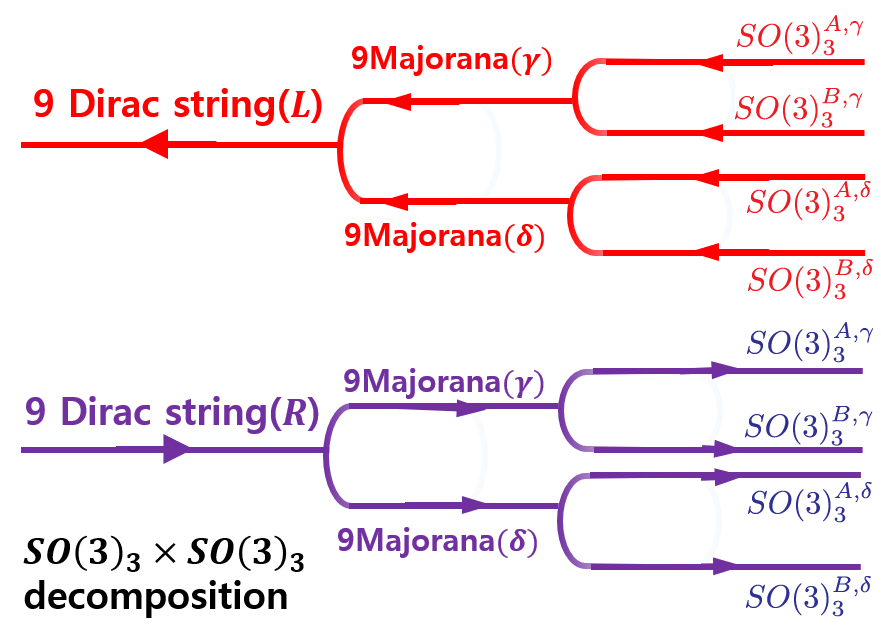
\includegraphics[width=0.7\textwidth]{SO3schematic}
	\centering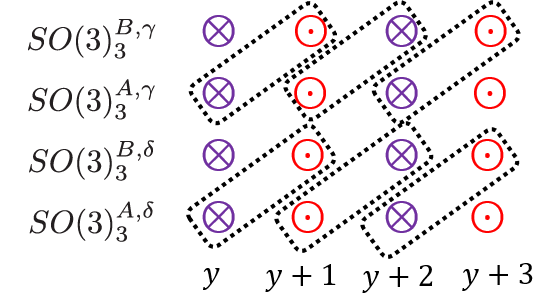
\includegraphics[width=0.7\textwidth]{SO3schematic2}
	\caption[(a) Schematic representations of the $SO(9)_1\supseteq SO(3)_3\times SO(3)_3$ decomposition. (b) Schematic figure of the $SO(3)_3\times SO(3)_3$ many-body gapping potential.]{(a) Schematic representations of the $SO(9)_1\supseteq SO(3)_3\times SO(3)_3$ decomposition. When $N=9$, we decompose each Dirac string into two Majorana fermions, $\gamma$ and $\delta$. Then each set of 9 Majorana fermions is decomposed into $SO(3)_3\times SO(3)_3$. (b) Schematic figure of the $SO(3)_3\times SO(3)_3$ many-body gapping potential. The boxes represent the current backscattering term between $SO(3)^{A,\psi}$ and $SO^{B,\psi}$ of adjacent wire in $y$ direction, for $\psi=\gamma,\delta$.}
	\label{Fig:SO3}
\end{figure}

We now define the two-body potential using $SO(3)_3$ current backscatterings \begin{align}\mathcal{H}_{\mathrm{int}}=u\sum_{xy}{\bf J}^{\gamma,A}_{x,y}\cdot{\bf J}^{\gamma,B}_{x,y+1}+{\bf J}^{\delta,A}_{x,y}\cdot{\bf J}^{\delta,B}_{x,y+1},\label{HintSO3}\end{align} where ${\bf J}=(J_{\mathsf{x}},J_{\mathsf{y}},J_{\mathsf{z}})$ are the $SO(3)_3$ current operators defined in Eq. \eqref{SO33currentdef}. Figure \ref{Fig:SO3} shows the schematic figure of the gapping potential. From Eq. \eqref{majoranaAFTR}, \eqref{majoranaG} and \eqref{majoranaT}, we see that the potential preserves the antiferromagnetic time-reversal, glide and lattice translation symmetry. The gapping potential does not admit a mean-field solution with fermion bilinear order parameters $i\langle\psi^a\psi^b\rangle$ like those in Eq. \eqref{Hinteven2}. Therefore, to present the order parameters of the interaction in Eq. \eqref{HintSO3}, we introduce a further fractionalization (also known as coset construction~\cite{bigyellowbook} in the CFT context) for each of the four sectors $C=A,B$ and $\psi=\gamma,\delta$ \begin{align}SO(3)_3\sim SO(2)_3\times\mathbb{Z}_6,\label{Z6parafermion}\end{align} where $\mathbb{Z}_6$ represents the parafermion coset CFT~\cite{FateevZamolodchikov82,ZamolodchikovFateev85} $SO(3)_3/SO(2)_3=SU(2)_6/U(1)_6$.

The decomposition is done by first grouping three pairs of Majorana fermions into three neutral Dirac fermions in each sector \begin{align}f^{A,\psi}_1&=\frac{\psi^1+i\psi^2}{\sqrt{2}},&f^{B,\psi}_1&=\frac{\psi^1+i\psi^4}{\sqrt{2}}\nonumber\\f^{A,\psi}_2&=\frac{\psi^4+i\psi^5}{\sqrt{2}},&f^{B,\psi}_2&=\frac{\psi^2+i\psi^5}{\sqrt{2}}\nonumber\\f^{A,\psi}_3&=\frac{\psi^7+i\psi^8}{\sqrt{2}},&f^{B,\psi}_3&=\frac{\psi^3+i\psi^6}{\sqrt{2}}\nonumber\end{align} and bosonize \begin{align}f^{C,\psi}_j\sim\exp\left(i\tilde\phi^{C,\psi}_j\right)\label{so(3)3bosonization}\end{align} for $j=1,2,3$, $C=A,B$ and $\psi=\gamma,\delta$. The bosonic $SO(2)_3=U(1)_6$ sector is generated by the diagonal combination \begin{align}\Phi^{C,\psi}=\frac{\tilde\phi^{C,\psi}_1+\tilde\phi^{C,\psi}_2+\tilde\phi^{C,\psi}_3}{3}.\end{align} This leaves behind the orthogonal compliment $\phi^{C,\psi}_{\sigma,j}=\tilde\phi^{C,\psi}_j-\Phi^{C,\psi}$ and the Majorana fermions $\psi^3,\psi^6,\psi^9$ for the $A$ sector or $\psi^7,\psi^8,\psi^9$ for the $B$ sector. They combine into the parafermions \begin{align}\begin{split}\Psi^{A,\psi}&=\frac{1}{\sqrt{3}}\left(e^{i\phi_{\sigma,1}^{A,\psi}}\psi^3+e^{i\phi_{\sigma,2}^{A,\psi}}\psi^6+e^{i\phi_{\sigma,3}^{A,\psi}}\psi^9\right)\\\Psi^{B,\psi}&=\frac{1}{\sqrt{3}}\left(e^{i\phi_{\sigma,1}^{B,\psi}}\psi^7+e^{i\phi_{\sigma,2}^{B,\psi}}\psi^8+e^{i\phi_{\sigma,3}^{B,\psi}}\psi^9\right)\end{split},\label{Z6parafermiondefinition}\end{align} which generate the $\mathbb{Z}_6$ sector. The conformal field theory structures of the $SO(2)_3$ and $\mathbb{Z}_6$ are discussed in Ref.~\cite{PhysRevB.94.165142} and will not be repeated here.

The coset construction in Eq. \eqref{Z6parafermion} allows the decomposition of the $SO(3)_3$ Kac-Moody current operators and consequently the potential in Eq. \eqref{HintSO3} \begin{align}\mathcal{H}_{\mathrm{int}}=3u\sum_{xy}\sum_{\psi=\gamma,\delta}e^{i(\Phi^{A,\psi}_{x,y}+\Phi^{B,\psi}_{x,y+1})}\Psi^{A,\psi}_{x,y+1}\Psi^{B,\psi}_{x,y+2}+h.c.,\label{HintZ6}\end{align}
where we have dropped the forward scatterings \begin{align}9u\sum_{xy}\sum_{\stackrel{C=A,B}{\psi=\gamma,\delta}}\partial_z\Phi^{C,\psi}_{x,y}\partial_z\Phi^{C,\psi}_{x,y+1}\end{align} from Eq. \eqref{HintSO3} that only renormalize the velocity for the boson in $SO(2)_3$. Order parameters are given by the ground state expectation values $\left\langle\Phi^{A,\psi}_{x,y}+\Phi^{B,\psi}_{x,y+1}\right\rangle$ and $\left\langle\Psi^{A,\psi}_{x,y}\Psi^{B,\psi}_{x,y+1}\right\rangle$, for $\psi=\gamma,\delta$. The symmetries defined in Eq. \eqref{majoranaAFTR}, \eqref{majoranaG} and \eqref{majoranaT} require \begin{align}\left\langle\Psi^{A,\psi}_{x,y}\Psi^{B,\psi}_{x,y+1}\right\rangle&=-\left\langle\Psi^{A,\psi}_{x,y+1}\Psi^{B,\psi}_{x,y+2}\right\rangle\nonumber\\&=-\left\langle\Psi^{A,\psi}_{x+1,y}\Psi^{B,\psi}_{x+1,y+1}\right\rangle\nonumber\\\left\langle\Psi^{A,\gamma}_{x,y}\Psi^{B,\gamma}_{x,y+1}\right\rangle&=-\left\langle\Psi^{A,\delta}_{x,y}\Psi^{B,\delta}_{x,y+1}\right\rangle\nonumber\\\left\langle\Psi^{A,\psi}_{x,y}\Psi^{B,\psi}_{x,y+1}\right\rangle&=-\left\langle\Psi^{A,\psi}_{x,y+1}\Psi^{B,\psi}_{x,y+2}\right\rangle\nonumber\\&=-\left\langle\Psi^{A,\psi}_{x+1,y}\Psi^{B,\psi}_{x+1,y+1}\right\rangle\nonumber\\\left\langle\Psi^{A,\gamma}_{x,y}\Psi^{B,\gamma}_{x,y+1}\right\rangle&=-\left\langle\Psi^{A,\delta}_{x,y}\Psi^{B,\delta}_{x,y+1}\right\rangle.\label{oddorderparameter}\end{align} Similar to Eq. \eqref{evenorderparameter} in the even case, the order parameters defined in Eq. \eqref{oddorderparameter} are not unique choices. For example, there are order parameters that correspond to non-Abelian twist fields in the $\mathbb{Z}_6$ sector that have quantum dimension greater than 1. However, they are not essential in the discussion of the symmetry-preserving gapping potential and are omitted.
%%
\subsection{$E_8$ unimodular gapping potential}\label{Chapter:E8}
In the previous section, we found that even and odd copies of the $3$D Dirac nodal superconductor can be gapped out by many-body gapping potentials, which support non-trivial topological order. In this section, we now focus on the special case when there are $N=16$ copies of the Dirac nodal superconductor exists. In this case, we can construct a many-body gapping potential by utilizing $SO(32)\sim E_8\times E_8$ decomposition, where $E_8$ is the largest exceptional simple Lie algebra. The $E_8\times E_8$ decomposition is atypical from the previous decompositions since the roots of the $E_8$ Lie algebra form an even unimodular lattice. Here, we show that this property of the $E_8$ algebra allows us to construct many-body gapping potential in the $3D$ Dirac nodal superconductor that does not possess topological order.

Before going into the details on the construction of the gapping term, we briefly explain the $E_8$ Kac-Moody algebra at level one using bosonized variables. In addition to 8 Cartan generators $\partial\phi_I$, $I=1,\ldots,8$, the $(E_8)_1$ algebra is generated by the vertex operators $E^{\boldsymbol\alpha}=e^{i\boldsymbol\alpha\cdot\boldsymbol\phi}$, where $\boldsymbol\alpha$ is a root vector of the $E_8$ lattice. The $E_8$ lattice $\mathcal{L}_{E_8}$ is an 8 dimensional lattice generated by 8 simple root vectors. It is an even unimodular lattice in the sense that the norm square $|{\bf v}|^2$ of a lattice vector is even, and the dual lattice $\mathcal{L}_{E_8}^\ast$, which consists of dual vectors ${\bf v}^\ast$ whose scalar product with any $E_8$ lattice vector ${\bf v}$ is integral, is the $E_8$ lattice itself. In particular, there are 240 root vectors $\boldsymbol\alpha$ with norm square $|\boldsymbol\alpha|^2=2$ so that the vertex operators $E^{\boldsymbol\alpha}$ have unit spin and represent the $E_8$ Kac-Moody current.

The total 240 roots separate into two distinct sets. The first set consists of $112=C^8_2\times4$ roots of $SO(16)$ and the second set consists of $128=2^7$ even spinors of $SO(16)$. The conventional choice of roots embeds them in the 8 dimensional Euclidean space. The $SO(16)$ roots are taken to be integral vectors with two and only two non-zero components, each being $\pm1$. The corresponding vertex operators $E^{\boldsymbol\alpha}$ are fermion bilinears $d_ad_b$, $d_ad_b^\dagger$, $d_a^\dagger d_b$ and $d_a^\dagger d_b^\dagger$, for $1\leq a<b\leq8$. The even spinors are represented by half-integral vectors $\boldsymbol\epsilon/2=(\epsilon_1/2,\ldots,\epsilon_8/2)$, where $\epsilon_a=\pm1$, with overall positive sign $\epsilon_1\ldots\epsilon_8=1$. They corresponds to spinor vertex operators $e^{i\boldsymbol\epsilon\cdot\boldsymbol\phi/2}$, which are products of half fermions. Within the 240 roots, one can pick a set of 8 linearly independent simple roots that generate the entire set. \begin{gather}\begin{pmatrix}|&\ldots&|\\\boldsymbol\alpha_1&\ldots&\boldsymbol\alpha_8\\|&\ldots&|\end{pmatrix}=\left(\begin{smallmatrix}
1 & 0 & 0 & 0 & 0 & 0 & 0 & -\frac{1}{2} \\
-1 & 1 & 0 & 0 & 0 & 0 & 0 & -\frac{1}{2} \\
0 & -1 & 1 & 0 & 0 & 0 & 0 & -\frac{1}{2} \\
0 & 0 & -1 & 1 & 0 & 0 & 0 & -\frac{1}{2} \\
0 & 0 & 0 & -1 & 1 & 0 & 0 & -\frac{1}{2} \\
0 & 0 & 0 & 0 & 1 & -1 & 0 & -\frac{1}{2} \\
0 & 0 & 0 & 0 & 0 & 1 & -1 & -\frac{1}{2} \\
0 & 0 & 0 & 0 & 0 & 0 & 1 & -\frac{1}{2} \end{smallmatrix}\right).\label{E8simpleroots0}\end{gather} Their scalar products $\boldsymbol\alpha_I\cdot\boldsymbol\alpha_J=(K_{E_8})_{IJ}$ recover by the Cartan matrix of $E_8$ \begin{align}K_{E_8}=\left(\begin{smallmatrix}2&-1&&&&&&\\-1&2&-1&&&&&\\&-1&2&-1&&&&\\&&-1&2&-1&&&\\&&&-1&2&-1&&-1\\&&&&-1&2&-1&\\&&&&&-1&2&\\&&&&-1&&&2\end{smallmatrix}\right).\label{KE8}\end{align}

Unfortunately, the above conventional choice of roots involves spinors that are combinations of half fermions, which are non-local. In order to realize the $E_8$ algebra as integral combination of local fermions, we first extend the 8 chiral Dirac fermions by an additional counter-propagating pair of non-chiral Dirac fermions. This can be achieved by using the vortex reconstruction whereby we pull the addition non-chiral pair from high-energy to low-energy. The reconstruction does not alter the chirality $c=8=9-1$ of a vortex, which now consists of 9 forward propagating Dirac fermions and 1 backward propagating one. The $E_8$ lattice is now embedded in a $10=1+9$ dimensional ``Minkowski" space with metric $\eta=\mathrm{diag}(-1,1,\ldots,1)$. The $E_8$ roots consists of a subset of integral vectors ${\bf v}$ with norm square ${\bf v}^T\eta{\bf v}=-v_0^2+v_1^2+\ldots+v_9^2=2$. We begin with the roots of $SU(8)$, $\boldsymbol\alpha_{SU(8)}={\bf e}_a-{\bf e}_b$, where $1\leq a,b\leq8$ and $a\neq b$. These roots correspond to the fermion bilinear vertex operators $E^{\boldsymbol\alpha_{SU(8)}}\sim d_ad_b^\dagger$ and they obey the operator product expansion that defines the $SU(8)$ Kac-Moody algebra at level 1, \begin{align}E^{\boldsymbol\alpha_{SU(8)}}(w)E^{-\boldsymbol\alpha_{SU(8)}}(w')&=1/(w-w')^2+\ldots,\nonumber\\E^{\boldsymbol\alpha_{SU(8)}}(w)E^{\boldsymbol\alpha'_{SU(8)}}(w')&=c_{\alpha\alpha'}E^{\boldsymbol\alpha''_{SU(8)}}(w')/(w-w')\nonumber\\&\;\;\;+\ldots,\end{align} if $\boldsymbol\alpha''_{SU(8)}=\boldsymbol\alpha'_{SU(8)}+\boldsymbol\alpha'_{SU(8)}$, or non-singular if otherwise, where $w\sim\tau+iz$ is the complex space-time parameter and the cocycle factor $c_{\alpha\alpha'}$ is a scalar phase.



These 56 roots can be extended to $SO(16)$ by including two 28-dimensional irreducible representations of $SU(8)$. The first corresponds to 28 positive root vectors $\boldsymbol\alpha_{(+{\bf 28})}=2{\bf e}_0+n_1{\bf e}_1+\ldots+n_8{\bf e}_8$, where two of $n_1,\ldots,n_8$ are 0's and the rest are 1's. The second corresponds to 28 negative roots $\boldsymbol\alpha_{(-{\bf 28})}=-2{\bf e}_0-n_1{\bf e}_1-\ldots-n_8{\bf e}_8$. Each forms a super-selection sector that is closed under the $SU(8)$ Kac-Moody algebra \begin{align}E^{\boldsymbol\alpha_{SU(8)}}(w)E^{\boldsymbol\alpha'_{(\pm{\bf 28})}}(w')=c_{\alpha\alpha'}E^{\boldsymbol\alpha''_{(\pm{\bf 28})}}(w')/(w-w')+\ldots\end{align} if $\boldsymbol\alpha''_{(\pm{\bf 28})}=\boldsymbol\alpha_{SU(8)}+\boldsymbol\alpha'_{(\pm{\bf 28})}$, or non-singular if otherwise. The root vectors are chosen so that $\boldsymbol\alpha_{(\pm{\bf28})}^T\eta\boldsymbol\alpha_{(\pm{\bf28})}=2$ so that the vertices $E^{\boldsymbol\alpha_{(\pm{\bf28})}}$ have spin 1. We label $\boldsymbol\alpha_{SO(16)}$ to be the 112 roots for $SO(16)$, and they consists of $\boldsymbol\alpha_{SO(16)}$ and $\boldsymbol\alpha_{(\pm{\bf28})}$.

Next, the 112 $SO(16)$ roots can be extended to the full $E_8$ by including two 56-dimensional irreducible representations of $SU(8)$ and the two 8-dimensional vector representations of $SU(8)$. The first irreducible representation that we include is associated with the 56 positive root vectors $\boldsymbol\alpha_{(+{\bf56})}={\bf e}_0+m_1{\bf e}_1+\ldots+m_8{\bf e}_8$, where three of $n_1,\ldots,n_8$ are 1's and the rest are 0's. The conjugate representation is associated with the 56 negative roots $\boldsymbol\alpha_{(-{\bf56})}=-{\bf e}_0-m_1{\bf e}_1-\ldots-m_8{\bf e}_8$. The 8 positive $SU(8)$ vectors are $\boldsymbol\alpha_{(+{\bf8})}=3{\bf e}_0+v_1{\bf e}_1+\ldots+v_8{\bf e}_8$, where all but one $v_a=1$ and the remaining is 2. The 8 negative $SU(8)$ vectors are the conjugate $\boldsymbol\alpha_{(-{\bf8})}=-3{\bf e}_0-v_1{\bf e}_1-\ldots-v_8{\bf e}_8$. We label $\boldsymbol\alpha_{\mathrm{spinor}}$ to be the $128=56+56+8+8$ additional vectors $\boldsymbol\alpha_{(\pm{\bf56})}$ and $\boldsymbol\alpha_{(\pm{\bf8})}$ that constitute the even spinor representation for the $SO(16)$ algebra. \begin{align}E^{\boldsymbol\alpha_{SO(16)}}(w)E^{\boldsymbol\alpha'_{\mathrm{spinor}}}(w')&=c_{\alpha\alpha'}E^{\boldsymbol\alpha''_{\mathrm{spinor}}}(w')/(w-w')\nonumber\\&\;\;\;+\ldots\end{align} if $\boldsymbol\alpha''_{\mathrm{spinor}}=\boldsymbol\alpha_{SO(16)}+\boldsymbol\alpha'_{\mathrm{spinor}}$, or non-singular if otherwise. The $E_8$ root vectors $\boldsymbol\alpha_{E_8}$ now consists of the 112 $\boldsymbol\alpha_{SO(16)}$'s and 128 $\boldsymbol\alpha_{\mathrm{spinor}}$'s.

The $240=112+128$ $E_8$ roots can be generated by the 8 simple roots \begin{gather}\begin{pmatrix}|&\ldots&|\\\boldsymbol\alpha_1&\ldots&\boldsymbol\alpha_8\\|&\ldots&|\end{pmatrix}=\left(\begin{smallmatrix}
0 & 0 & 0 & 0 & 0 & 0 & 0 & 1 \\
1 & 0 & 0 & 0 & 0 & 0 & 0 & 0 \\
-1 & 1 & 0 & 0 & 0 & 0 & 0 & 0 \\
0 & -1 & 1 & 0 & 0 & 0 & 0 & 0 \\
0 & 0 & -1 & 1 & 0 & 0 & 0 & 0 \\
0 & 0 & 0 & -1 & 1 & 0 & 0 & 0 \\
0 & 0 & 0 & 0 & -1 & 1 & 0 & 1 \\
0 & 0 & 0 & 0 & 0 & -1 & 1 & 1 \\
0 & 0 & 0 & 0 & 0 & 0 & -1 & 1 \\
0 & 0 & 0 & 0 & 0 & 0 & 0 & 0 \end{smallmatrix}\right).\label{E8simpleroots}\end{gather} Their scalar products $\boldsymbol\alpha_I\cdot\eta\boldsymbol\alpha_J=(K_{E_8})_{IJ}$ recover the Cartan matrix of $E_8$ defined in Eq. \eqref{KE8}.

The embedding into the Minkowski space $\mathbb{R}^{1,9}$ guarantees a counter-propagating pair of redundant modes. They are the Dirac fermions $f_R\sim e^{i\boldsymbol\alpha_f^R\cdot\boldsymbol\phi}$ and $f_L\sim e^{i\boldsymbol\alpha_f^L\cdot\boldsymbol\phi}$, where $\boldsymbol\alpha^R_f={\bf e}_9$ and $\boldsymbol\alpha^L_f=3{\bf e}_0+{\bf e}_1+\ldots+{\bf e}_8$. They are fermionic because of the unit norm squares $\boldsymbol\alpha^R_f\cdot\eta\boldsymbol\alpha^R_f=1$ and $\boldsymbol\alpha^L_f\cdot\eta\boldsymbol\alpha^L_f=-1$. They decoupled from each other as well as the $E_8$ roots since $\boldsymbol\alpha_{E_8}\cdot\eta\boldsymbol\alpha^{R/L}_f=\boldsymbol\alpha^R_f\cdot\eta\boldsymbol\alpha^L_f=0$. Grouping $\boldsymbol\alpha^{R/L}_f$ with the $E_8$ simple roots in Eq. \eqref{E8simpleroots}, the $10\times10$ matrix $A=(\boldsymbol\alpha_1,\ldots,\boldsymbol\alpha_8,\boldsymbol\alpha^R_f,\boldsymbol\alpha^L_f)$ is unimodular (i.e.~$|\det(A)|=1$), and may be decomposed into block diagonal form as \begin{align}A^T\eta A=\begin{pmatrix}K_{E_8}&\\&\sigma_z\end{pmatrix},\label{AAT}\end{align} where $\sigma_z=\mathrm{diag}(1,-1)$.

Having completing the formal definition of the $E_8$ algebra, we now construct the gapping potential, which consists of inter-vortex $E_8$ current backscattering and intra-vortex fermion backscattering $f_Rf_L^\dagger$. Each vortex has chirality $c=16$ and carries 16 chiral Dirac fermions. We extend by vortex reconstruction to 18 forward moving Dirac fermions plus 2 backward moving ones. They can be bipartitioned into two groups of $9+1$, each of which can be transformed unimodularly into $E_8\times U(1)^R\times U(1)^L$, as has been explained above. In a similar fashion to our the previous discussions, we label the two groups by $A$ and $B$. The gapping potential is \begin{align}H&=-\frac{u_{\mathrm{inter}}}{2}\sum_{xy}\sum_{\boldsymbol\alpha_{E_8}}E^{A,\boldsymbol\alpha_{E_8}}_{x,y}E^{B,\boldsymbol\alpha_{E_8}}_{x,y+1}\nonumber\\&\;\;\;-\frac{u_{\mathrm{intra}}}{2}\sum_{xy}\sum_{C=A,B}(f_R^Cf_L^C+h.c.)\nonumber\\&=-u_{\mathrm{inter}}\sum_{xy}\sum_{\boldsymbol\alpha_{E_8}}\cos\left[\boldsymbol\alpha_{E_8}\cdot(\boldsymbol\phi^A_{x,y}+\boldsymbol\phi^B_{x,y+1})\right]\nonumber\\&\;\;\;-u_{\mathrm{intra}}\sum_{xy}\sum_{C=A,B}\cos\left(\boldsymbol\alpha^R_f\cdot\boldsymbol\phi^C_{xy}+\boldsymbol\alpha^L_f\cdot\boldsymbol\phi^C_{xy}\right)\label{E8sinegordon}\end{align} where the first sum runs over all 240 $E_8$ roots $\boldsymbol\alpha_{E_8}$.

All terms preserve the symmetries that we have defined in Eq. \eqref{bosonsymmtrans}. The angle order parameters $\Theta^{\boldsymbol\alpha_{E_8}}_{x,y+1/2}=\boldsymbol\alpha_{E_8}\cdot(\boldsymbol\phi^A_{x,y}+\boldsymbol\phi^B_{x,y+1})$ that appear in the inter-vortex term obey the symmetry relations \begin{align}T_A\Theta^{\boldsymbol\alpha_{E_8}}_{x,y+1/2}(z)T_A^{-1}&=-\Theta^{\boldsymbol\alpha_{E_8}}_{x,y+3/2}(z)+\pi\boldsymbol\alpha_{E_8}\cdot{\bf t}\nonumber\\G\Theta^{\boldsymbol\alpha_{E_8}}_{x,y+1/2}(z)G^{-1}&=-\Theta^{\boldsymbol\alpha_{E_8}}_{x+1,y+1/2}(-z)+\pi\boldsymbol\alpha_{E_8}\cdot{\bf t}\nonumber\\\mathsf{t}_{11}\Theta^{\boldsymbol\alpha_{E_8}}_{x,y+1/2}(z)\mathsf{t}_{11}^{-1}&=\Theta^{\boldsymbol\alpha_{E_8}}_{x+1,y+3/2}(z)\nonumber\\\mathsf{t}_{\bar{1}1}\Theta^{\boldsymbol\alpha_{E_8}}_{x,y+1/2}(z)\mathsf{t}_{\bar{1}1}^{-1}&=\Theta^{\boldsymbol\alpha_{E_8}}_{x-1,y+3/2}(z),\end{align} where ${\bf t}=(1,1,\ldots,1)^T$. The intra-vortex ones $\Theta^C_{x,y}=(\boldsymbol\alpha^R_f+\boldsymbol\alpha^L_f)\cdot\boldsymbol\phi^C_{xy}$, for $C=A,B$, obey \begin{align}T_A\Theta^C_{x,y}(z)T_A^{-1}&=-\Theta^C_{x,y+1}(z)+\frac{1-(-1)^{x+y}}{2}\pi(\boldsymbol\alpha^R_f+\boldsymbol\alpha^L_f)\cdot{\bf t}\nonumber\\G\Theta^C_{x,y}(z)G^{-1}&=-\Theta^C_{x+1,y}(-z)+\frac{\pi}{2}(\boldsymbol\alpha^R_f+\boldsymbol\alpha^L_f)\cdot{\bf t}\nonumber\\\mathsf{t}_{11}\Theta^C_{x,y}(z)\mathsf{t}_{11}^{-1}&=\Theta^C_{x+1,y+1}(z)\nonumber\\\mathsf{t}_{\bar{1}1}\Theta^C_{x,y}(z)\mathsf{t}_{\bar{1}1}^{-1}&=\Theta^C_{x-1,y+1}(z).\end{align} For the $E_8$ order parameters, $\boldsymbol\alpha_{E_8}\cdot{\bf t}=0,\pm4,\pm8,\pm12$ and, therefore, the inter-vortex sine-Gordon terms in Eq. \eqref{bosonsymmtrans} are symmetric, since $\cos(-\Theta+2m\pi)=\cos\Theta$. The intra-vortex terms in Eq. \eqref{bosonsymmtrans} are also symmetric because $(\pi/2)(\boldsymbol\alpha^R_f+\boldsymbol\alpha^L_f)\cdot{\bf t}=6\pi$. The ground state expectation values $\left\langle\Theta^{\boldsymbol\alpha_{E_8}}_{x,y+1/2}\right\rangle$ transform consistently according to the symmetries (c.f.~Eq.\eqref{evenorderparameter} for the even $N$ case). The fermionic order parameters $\left\langle\Theta^C_{x,y}\right\rangle$ transform consistently up to large gauge transformation $\left\langle\Theta^C_{x,y}\right\rangle\equiv\left\langle\Theta^C_{x,y}\right\rangle+2\pi$ originated from the gauge redundancy $d^a\sim e^{i\phi^a}=e^{i(\phi^a+2\pi)}$.



\begin{figure}[htbp]
	\centering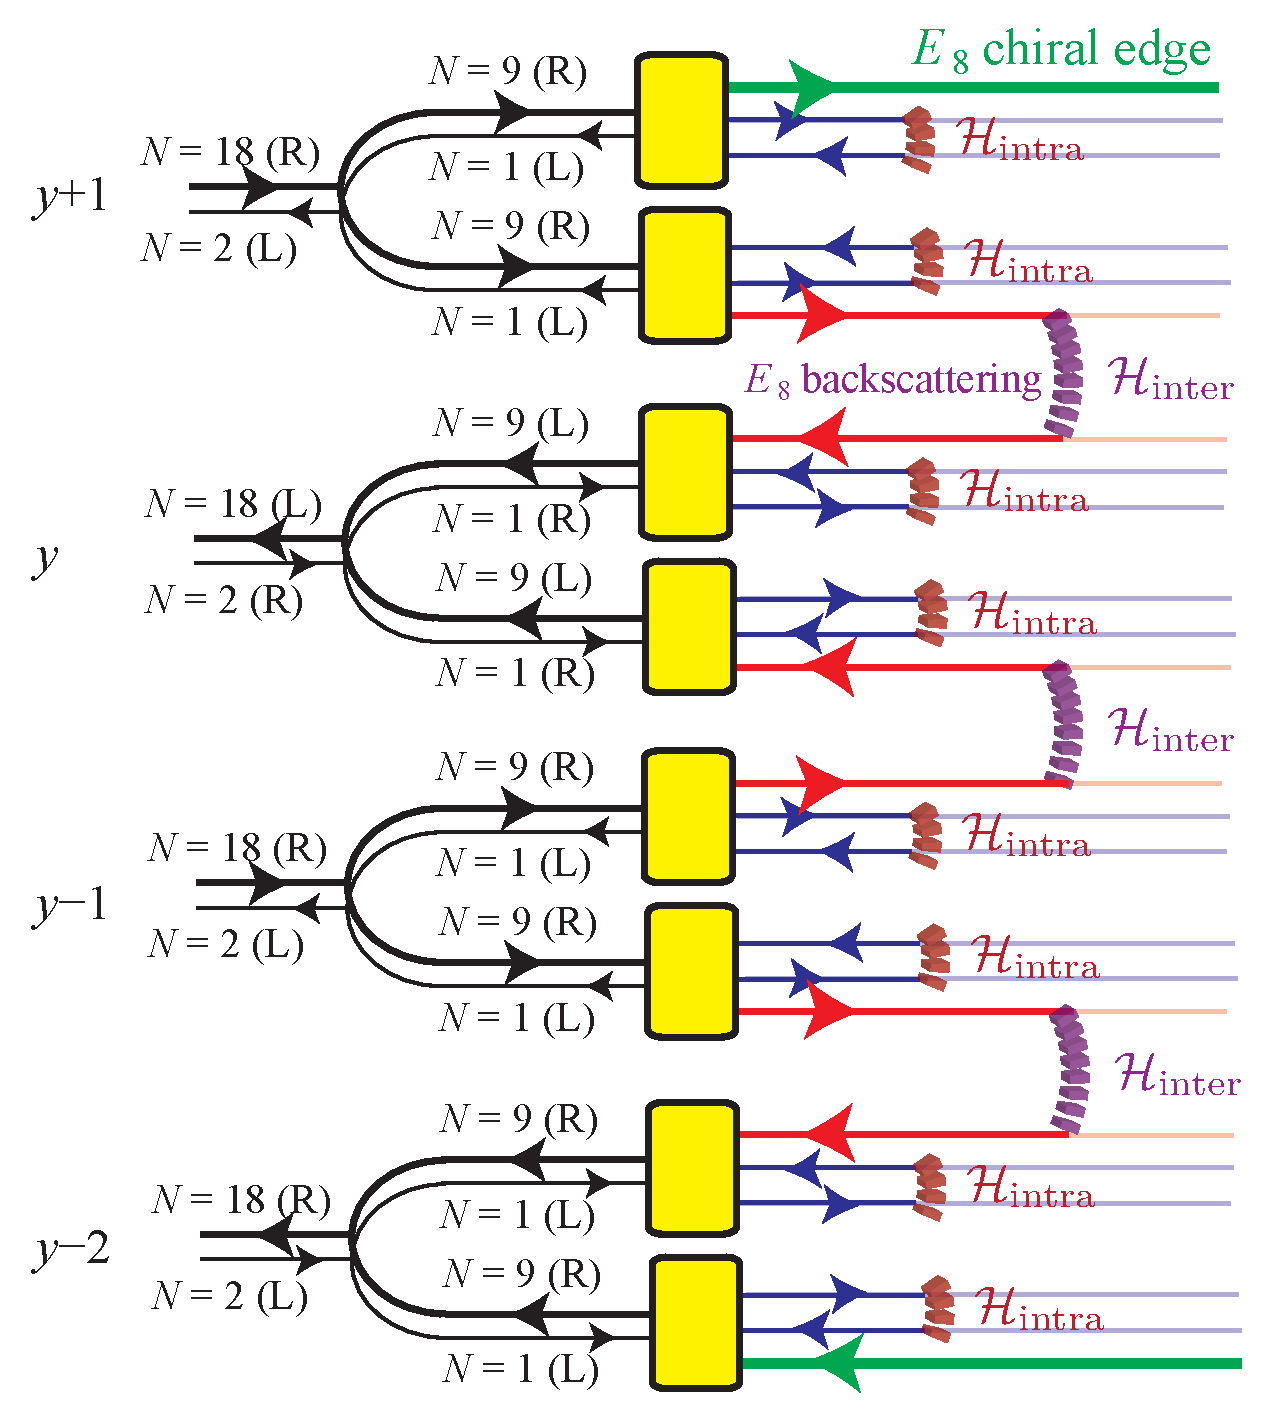
\includegraphics[width=0.8\textwidth]{E8schematic.pdf}
	\caption[Schematic figure of $E_8$ decomposition and gapping interaction.]{Schematic figure of $E_8$ decomposition and gapping interaction. Dirac modes (black lines) along each vortex $y$ are decomposed into two sets of $E_8$ chiral CFT (red lines) and two counter-propagating pairs of Dirac fermions (blue lines) by the basis transformation $A$ in Eq. \eqref{AAT} (yellow boxes). The $E_8$ backscattering terms $\mathcal{H}_{\mathrm{inter}}$ and the fermion backscattering $\mathcal{H}_{\mathrm{intra}}$ are defined in Eq. \eqref{E8sinegordon}. Uncoupled $E_8$ chiral CFTs are left along the boundaries of an open system, while the bulk mimics the $E_8$ quantum Hall state.}\label{fig:E8schematic}
\end{figure}

The angle variables in Eq. \eqref{E8sinegordon} satisfy the Haldane nullity condition, and the sine-Gordon interaction generates a symmetry preserving gap in the energy spectrum. In Eq. \eqref{E8sinegordon}, we considered the $E_8$ backscattering term, coupling with adjacent wires in $\hat{y}$-direction. In the absence of the single-body hopping but Eq. \eqref{E8sinegordon}, the arrays of the Dirac strings form a coupled $2D$ layer in $yz$ plane, possessing a finite bulk gap. We now consider open boundary condition in $y$ direction as shown in Fig.~\ref{fig:E8schematic}. Along the boundary of the $2D$ layer, a chiral $E_8$ edge state is left uncoupled and remains gapless, since there is no counter-propagating adjacent Dirac string to pair with. Therefore, each $2D$ layer resembles a quantum Hall state carrying a $E_8$ CFT as its edge theory in low-energy. As a result, the $2D$ bulk topological order and the bulk excitations of the layers can be inferred from the $E_8$ edge state.

The low energy effective theory for the $E_8$ quantum Hall states are described by Chern-Simons theory with $K_{E_8}$ matrix whose action is given as,
\begin{gather}
\mathcal{S}_{cs}=\frac{1}{4\pi}\sum_{I,J}\int dx^2  (K_{E_8})_{IJ} \epsilon^{\mu\nu\lambda} a_{I,\mu}\partial_{\nu}a_{J,\lambda}-\sum_{I}a_{\mu,I}j_{\mu, I}
\end{gather}
and $K_{E_8}$ is the Cartan matrix of $E_8$ defined in Eq. \eqref{KE8}. Here, $a_I$ is $I^{\mathrm{th}}$ Abelian gauge field whose classical equation of the motion yields the Hall effect. $K_{E_8}$ matrix contains the information of the bulk quasi-particle excitations and the corresponding edge theory. To be specific, the topological order or the ground state degeneracy of the corresponding bulk theory is identified as the determinant of $K$ matrix. It can be seen that the bulk topological order of $E_8$ state is trivial ($\det(E_8)=1$), since it is unimodular. Consequently, the system only supports local exitations with non-fractional statistics.

We have constructed the symmetry preserving many-body gapped phase with no topological order. It is important to note that the presence of such a phase is intimately related to the properties of even unimodular lattice. %Firstly to be symmetry preserving, the sine-Gordon term should contain even integrals of the original Dirac wire. This indicates that the norm of the roots must be even. Secondly, the determinant of $K$ matrix must be $1$, to ensure the absence of the topological order. The set of the roots which satisfies these two conditions necessarily forms an even unimodular lattice.
The $E_8$ lattice is the minimal even unimodular lattice, that appears in $8$ dimensions. Other even unimodular lattices, such as the Leech lattice in dimension 24, that appear in higher dimensions can be similarly utilized to construct the topologically trivial gapping potential.


%
\chapter{Model 3: Interacting Weyl Semimetal with two Weyl nodes}\label{chap:Model3}

So far, we have been discussing the gapping of the Dirac semimetal while preserving the \AFTR and $C_2$ symmetries. In this subsection, we focus on an opposite aspect of the symmetric many-body interaction -- the enabling of a (semi)metallic phase that is otherwise forbidden by symmetries in the single-body setting. We noticed in Subsec.~\ref{sec:anomaly} that the pair of momentum-separated Weyl points in Fig.~\ref{fig:Weylspectrum} is anomalous. In fact, it is well-known already that Weyl nodes~\cite{Murakami2007,WanVishwanathSavrasovPRB11,YangLuRan11,burkovBalenstPRL11,Ashvin_Weyl_review}, if separated in momentum space, must come in multiples of four in a lattice translation and time reversal symmetric three dimensional non-interacting system. 

This no go theorem can be rephrased into a feature. \begin{enumerate}\item If the low energy excitations of a \TR symmetric lattice (semi)metal in three dimensions consists of one pair of momentum-separated Weyl nodes, then the system must involve many-body interaction.\end{enumerate} We refer to this \TR and lattice translation symmetric strongly-correlated system as an interaction-enabled topological Dirac (semi)metal. We assume the Weyl nodes are fixed at two \TR invariant momenta, and therefore they are stable against symmetry-preserving deformations. Otherwise, if the Weyl nodes are not located at high symmetry points, they can be moved and pair annihilated. Also, as explained in the beginning of Sec.~\ref{sec:DiracSemimetal} and contrary to the more common contemporary terminology, we prefer to call the (semi)metal ``Dirac" rather than ``Weyl" because of the doubling. Perhaps more importantly, we propose the following conjecture. \begin{enumerate}\addtocounter{enumi}{1}\item Beginning with the interaction-enabled Dirac (semi)metal, {any} single-body symmetry-breaking mass must lead to a 3D gapped topological phase that cannot be adiabatically connected to a band insulator.\end{enumerate} We suspect this statement can be proven by a filling argument similar to that of Hasting-Oshikawa-Lieb-Schultz-Mattis~\cite{LiebSchultzMattis61,Oshikawa00,Hastings04}, and may already be available in Ref.~\cite{WatanabePoVishwanath17} by Watanabe, Po and Vishwanath. This conjecture applies to the coupled wire situation where the gapped phase is long-range entangled and supports fractional excitations. Its topological order is out of the scope of this article, but will be presented in a future work~\cite{SirotaRazaTeoappearsoon}. In a broader perspective, this type of statements may provide connections between strongly-interacting and non-interacting phases and help understanding quantum phase transitions of long-range entangled 3D phases from that of single-body band insulating ones.

Before discussing the three dimensional case, we make the connection to a few known interaction-enabled topological phases with or without an energy gap in low dimensions. First, zero energy Majorana fermions $\gamma_j=\gamma_j^\dagger$ in a true zero dimensional non-interacting (spinless) \TR symmetric system must bipartite into an equal number of positive chiral ones $\mathcal{T}\gamma_j\mathcal{T}^{-1}=+\gamma_j$ and negative chiral ones $\mathcal{T}\gamma_l\mathcal{T}^{-1}=-\gamma_l$. Fidkowski and Kitaev showed in Ref.~\cite{FidkowskiKitaev10} that under a combination of two-body interactions, eight Majoranas with the same chirality can acquire a \TR preserving mass and be removed from low energy. This leaves behind a collection of zero energy Majoranas that have a non-trivial net chirality of eight. Second, all $(1+1)$D \TR symmetric topological BDI superconductors~\cite{SchnyderRyuFurusakiLudwig08,Kitaevtable08,QiHughesRaghuZhang09,HasanKane10,QiZhangreview11,RMP} must break inversion because the zero energy Majorana boundary modes must have opposite chiralities at opposite ends. The Fidkowski-Kitaev interaction however allows one to construct a non-trivial $(1+1)$D topological model that preserves both \TR and inversion but at the same time supports four protected Majorana zero modes at each end~\cite{LapaTeoHughes14}. Third, a single massless Dirac fermion in $(2+1)$D is anomalous in a (spinful) \TR and charge $U(1)$ preserving non-interacting lattice system. On the other hand, it can be enabled by many-body interactions. For instance, when one of the two opposing surfaces of a topological insulator slab is gapped by symmetry-preserving interactions~\cite{WangPotterSenthilgapTI13,MetlitskiKaneFisher13b,ChenFidkowskiVishwanath14,BondersonNayakQi13}, a single massless Dirac fermion is left behind on the opposite surface as the only gapless low energy degrees of freedom of the quasi-$(2+1)$D system. Similar slab construction can be applied to the superconducting case, and interactions can allow any copies of massless Majorana fermions to manifest in $(2+1)$D with the presence of (spinful) \TR symmetry.

On the contrary, there are anomalous gapless fermionic states that cannot be enabled even by strong interactions. Chiral fermions that only propagate in a single direction cannot be realized in a true $(1+1)$D lattice system. They can only be supported as edge modes of $(2+1)$D topological phases such as quantum Hall states~\cite{Wenedgereview} or chiral $p_x+ip_y$ superconductors~\cite{Volovik99,ReadGreen}. Otherwise, they would allow heat transfer~\cite{KaneFisher97,Cappelli01,Kitaev06} from a low temperature reservoir to a high temperature one, thereby violating the second law of thermodynamics. Similarly, a single massless Weyl fermion can only be present as the $(3+1)$D boundary state of a $(4+1)$D topological bulk~\cite{ZhangHu01,BernevigChernHuToumbasZhang02,QiHughesZhang08,SchnyderRyuFurusakiLudwig08,Kitaevtable08}. It cannot exist in a true $(3+1)$D lattice system~\cite{Nielsen_Ninomiya_1981,NielsenNinomiyaPLB1981}, or otherwise under a magnetic field there would be unbalanced chiral fermions propagating along the field direction that constitute the ABJ-anomaly~\cite{Adler69,BellJackiw69,NielsenNinomiya83}.

\begin{figure}[htbp]
	\centering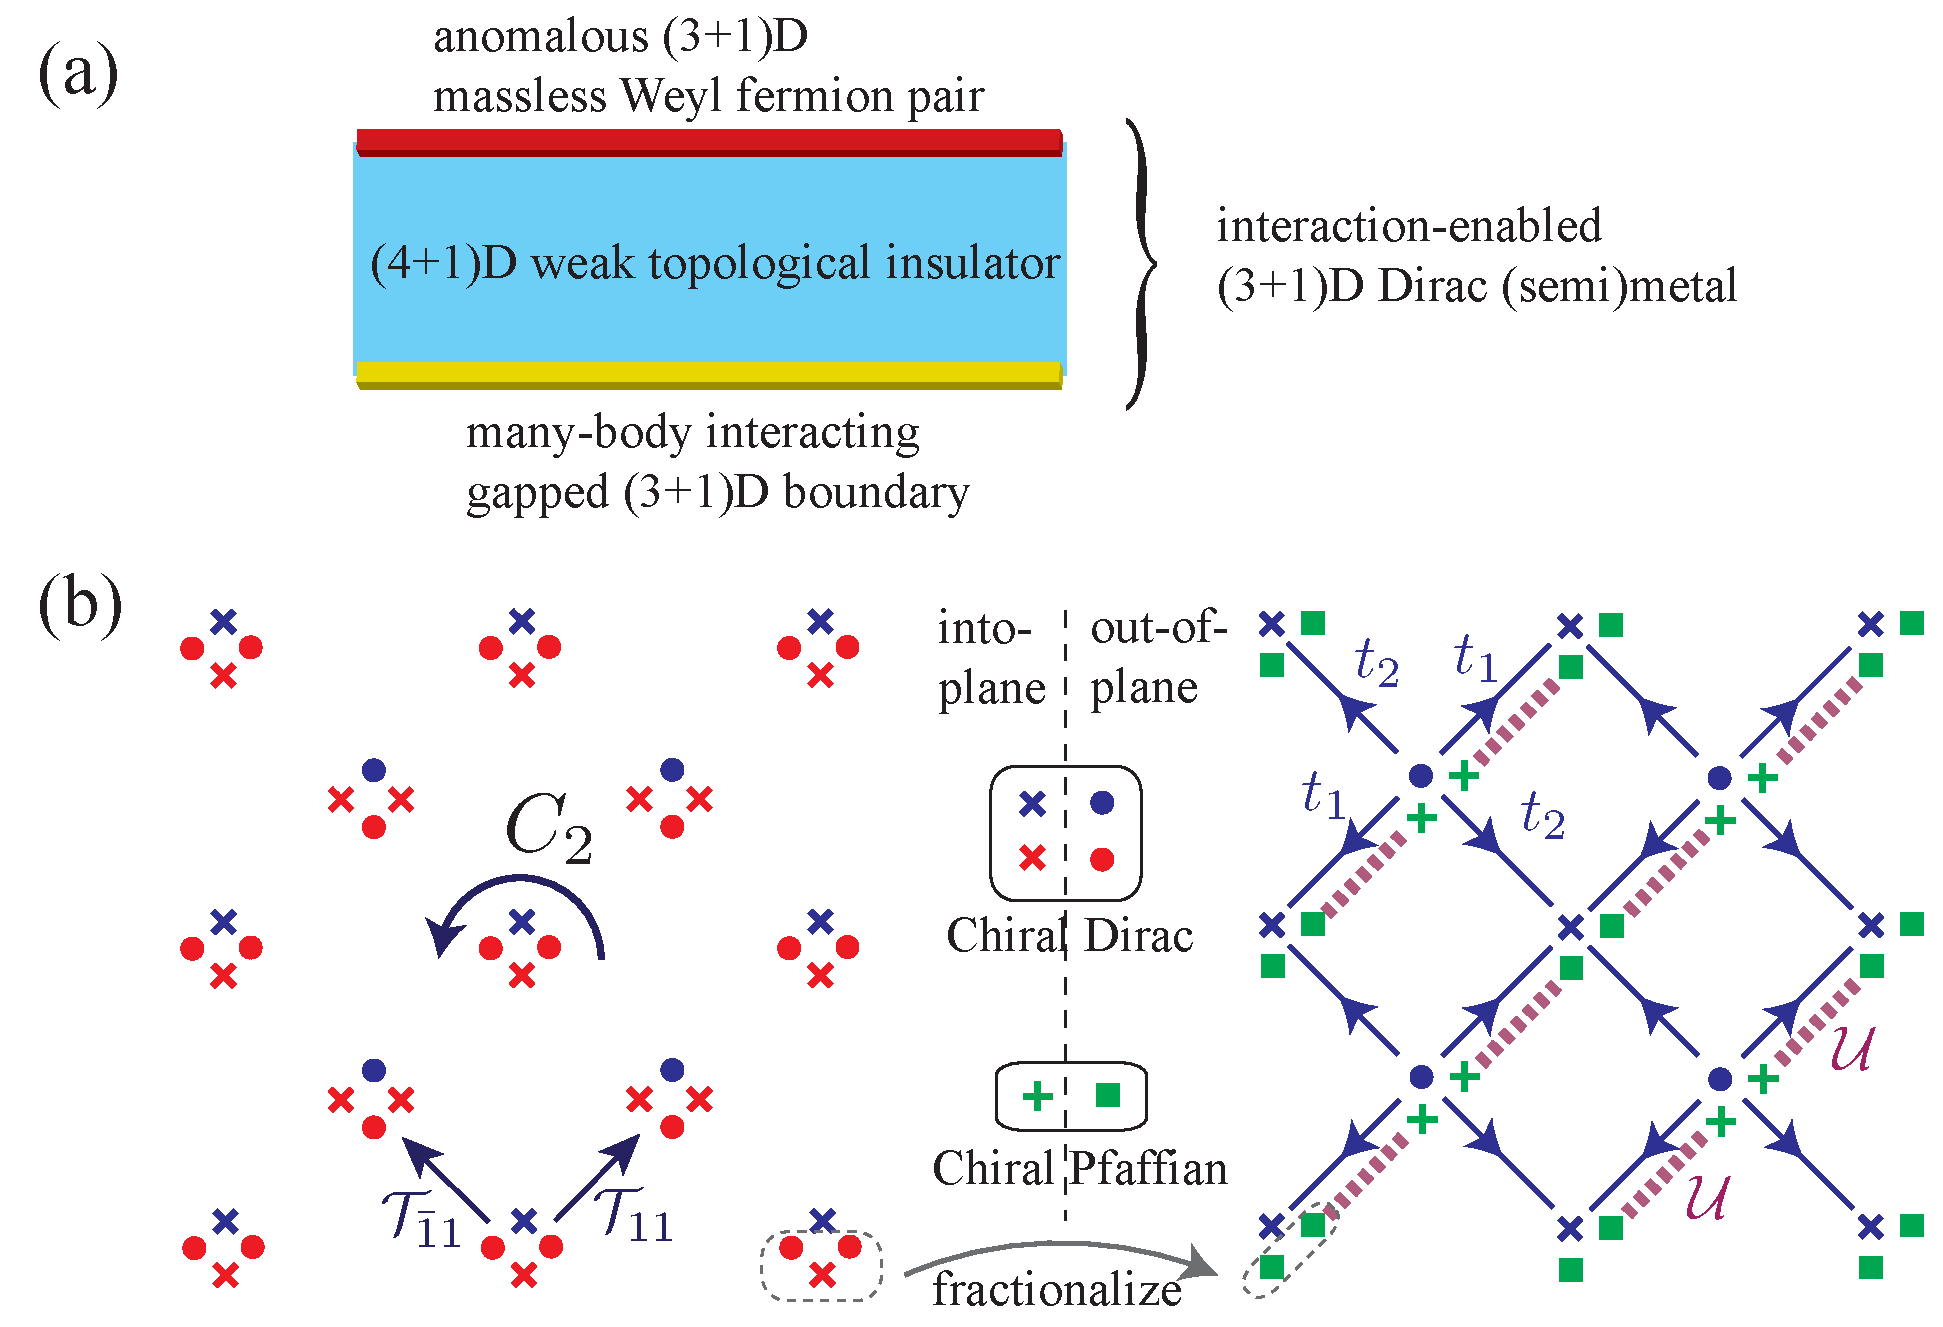
\includegraphics[width=0.94\textwidth]{intenable}
	\caption[(a) A quasi-$(3+1)$D interaction-enabled Dirac (semi)metal constructed by a 4D slab of WTI. (b) Coupled wire model of an anomalous Dirac (semi)metal.]{(a) A quasi-$(3+1)$D interaction-enabled Dirac (semi)metal constructed by a 4D slab of WTI. (b) Coupled wire model of an anomalous Dirac (semi)metal enabled by interaction with $C_2$ rotation and both AFTR $\mathcal{T}_{11},\mathcal{T}_{\bar{1}1}$ symmetries.}\label{fig:intenable}
\end{figure}

In this section, we focus on the simplest anomalous gapless fermionic states in $(3+1)$D that can be enabled by interactions. As eluded in Sec.~\ref{sec:holproj4D}, a weak topological insulator in $(4+1)$D can support the anomalous energy spectrum in Fig.~\ref{fig:Weylspectrum} on its boundary so that a pair of opposite Weyl points sit at two distinct \TRIM on the boundary Brillouin zone. A 4D \WTI slab, where the fourth spatial dimension is open and the other three are periodic, has two $(3+1)$D boundaries and each carries a pair of Weyl fermions. The coupling between the two pairs of Weyl fermions are suppressed by the system thickness and bulk energy gap. By introducing symmetry-preserving gapping interactions on the bottom surface, the anomalous gapless fermionic state is left behind on the top surface and is enabled in this quasi-$(3+1)$D setting (see Fig.~\ref{fig:intenable}(a)).

Inspired by this construction, we propose a true $(3+1)$D coupled wire model which has the anomalous energy spectrum in Fig.~\ref{fig:Weylspectrum} and preserves the \AFTR symmetries in both $\mathcal{T}_{11}$ and $\mathcal{T}_{\bar{1}1}$ directions as well as the $C_2$ (screw) rotation symmetry. The model is summarized in Fig.~\ref{fig:intenable}(b). It consists of a checkerboard array of electronic wires, where each wire has two chiral Dirac channels propagating into-paper and another two propagating out-of-paper. Contrary to the model considered in Sec.~\ref{sec:DiracSemimetal}, here the net chirality on each wire cancels and therefore the wires are true $(1+1)$D systems without being supported by a higher dimensional bulk. Using the splitting scheme described in Sec.~\ref{sec:gluing}, along each wire, one can fractionalize a group of three Dirac channels {\color{red}$\bullet\bullet\times$} ({\color{red}$\times\times\bullet$}) into a pair of co-propagating chiral Pfaffian channels {\color{green}$\blacksquare\blacksquare$} (resp.~{\color{green}$++$}). The two Pfaffian channels then can be backscattered in opposite directions using the many-body interaction $\mathcal{U}$ (dashed purple lines) described in Sec.~\ref{sec:interactionmodels}. This introduces an excitation energy gap that removes three Dirac channels per wire from low energy. Lastly, single-body backscatterings $t_1,t_2$ (solid directed blue lines) among the remaining Dirac channels {\color{blue}$\bullet\times$} described in \eqref{WeylTBHam} and Fig.~\ref{fig:WeylTB} give rise to the low-energy Weyl spectrum in Fig.~\ref{fig:Weylspectrum}. Since the many-body interaction $\mathcal{U}$ and the single-body backscatterings $t_1,t_2$ preserve the $C_2$ rotation and both \AFTR symmetries $\mathcal{T}_{11}$ and $\mathcal{T}_{\bar{1}1}$, the model describes an interaction-enabled anomalous (semi)metal that is otherwise forbidden in a non-interacting non-holographic setting. 

The non-local anti-ferromagnetic nature of the time reversal symmetry is built-in in the present coupled wire model. We speculate in passing that a local conventional \TR symmetric Dirac (semi)metallic phase consisting of a single pair of momentum-space-separated Weyl nodes may also be enabled by interaction. On one hand, the \AFTR symmetry could be restored to a local \TR symmetry by ``melting" the checkerboard wire array. On the other hand, there could also be an alternative wire configuration that facilitates a coupled wire model with a local conventional \TR symmetry.

Lastly, we gap the interaction-enabled Dirac semimetallic model (Fig.~\ref{fig:intenable}) by a symmetry-breaking single-body mass. This can be achieved by introducing electronic backscattering terms that dimerize the remaining Dirac channels {\color{blue}$\bullet\times$}, and were described by \eqref{DiracTBHam} in Sec.~\ref{sec:brokensymmetry}. The resulting state is an insulating $(3+1)$D topological phase with long-range entanglement. For instance, each diagonal layer gapped by the many-body interaction $\mathcal{U}$ has the identical topological order of the $\mathcal{T}$-Pfaffian surface state of a topological insulator. 

\section{Fractional Surface States}\label{sec:fracsurface}



In Sec.~\ref{sec:fermiarc1}, we discussed the surface states of the single-body coupled Dirac wire model \eqref{WeylTBHam} (see also Fig.~\ref{fig:WeylTB}). In particular, we showed in Fig.~\ref{fig:SurfaceStates1bdy} that an \AFTR symmetry preserving surface hosts open chiral Dirac channels, which connect and leak into the 3D (semi)metallic bulk. Earlier in this section, we discussed the effects of many-body interaction, which leads to two possible phases: (a) a gapped topological phase (see Sec.~\ref{sec:interactionmodels}) that preserves one of the two \AFTR symmetries, say $\mathcal{T}_{11}$, and (b) a gapless interaction-enabled Dirac semimetal (see Sec.~\ref{sec:intenable}) that preserves the $C_2$ rotation and both \AFTR symmetries $\mathcal{T}_{11}$ and $\mathcal{T}_{\bar{1}1}$. Here, we describe the boundary states of the two interacting phases on a surface closed under the symmetries.

\begin{figure}[htbp]
	\centering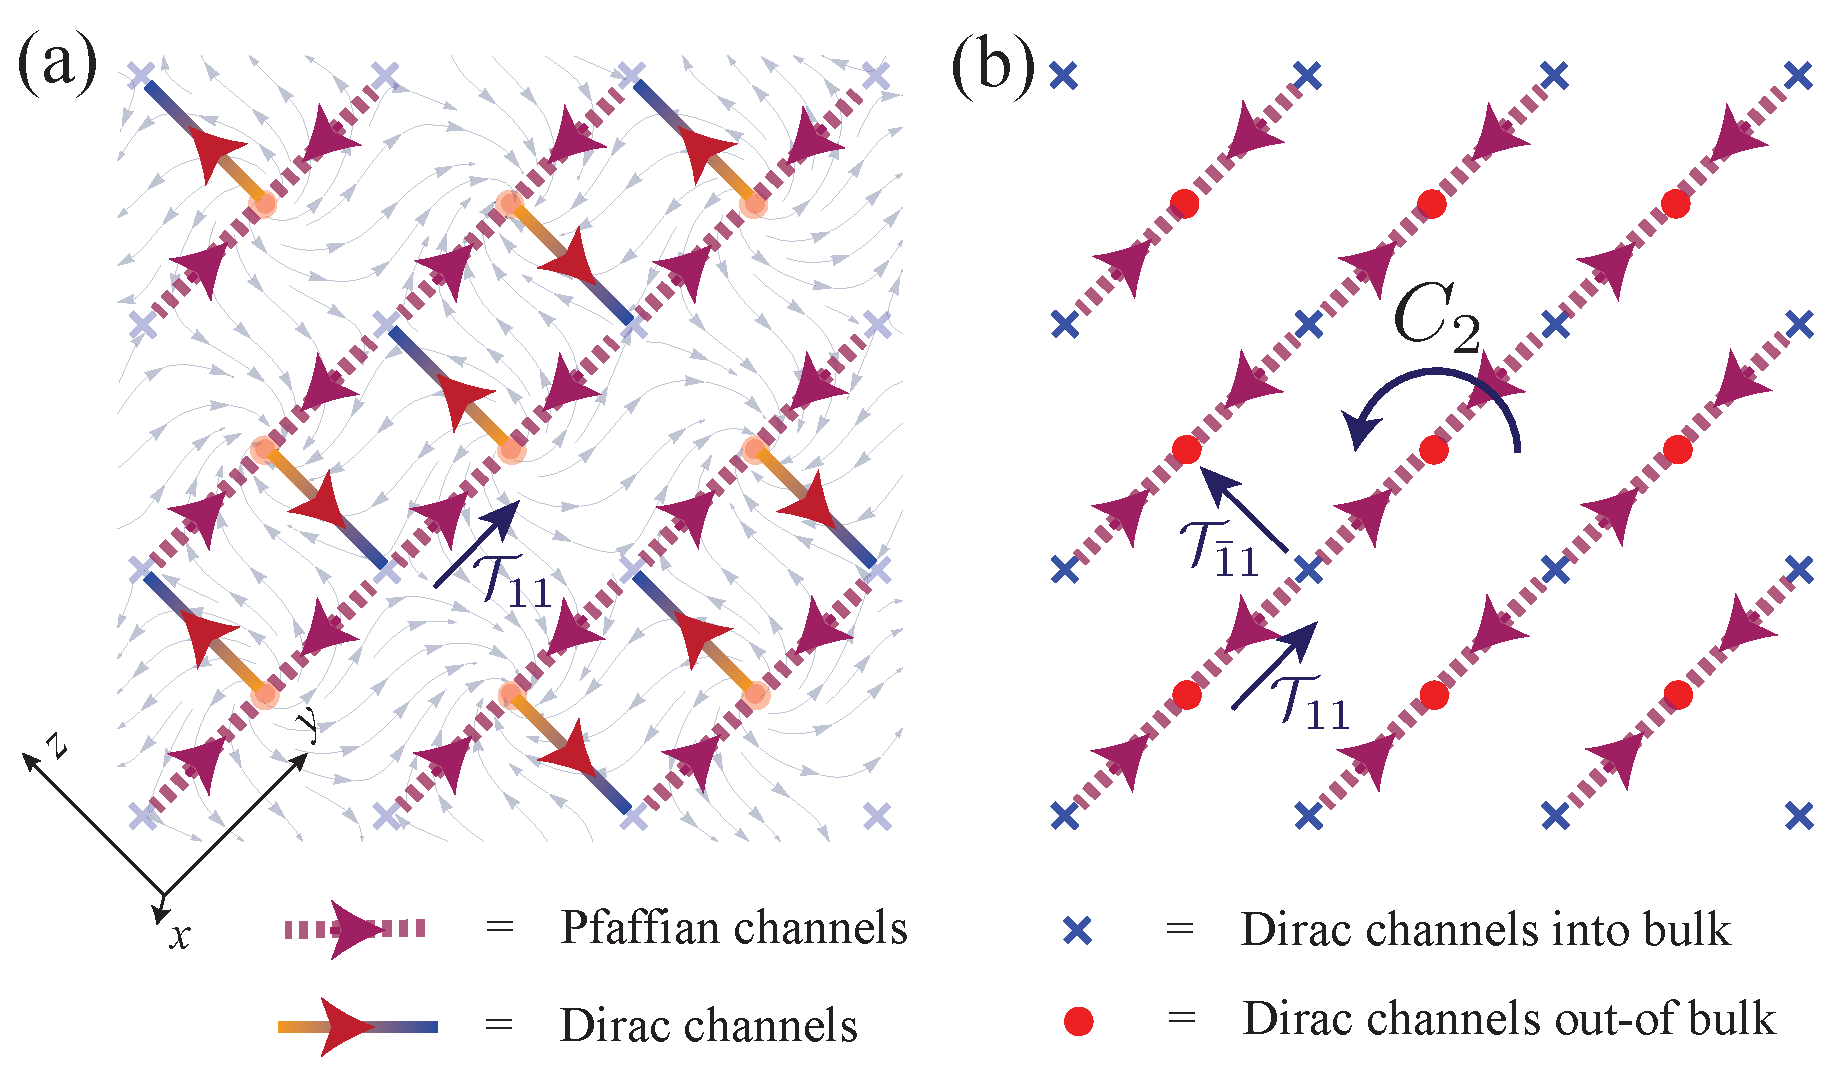
\includegraphics[width=0.96\textwidth]{SurfaceStates}
	\caption[Fractional surface states.]{Fractional surface states of (a) a 3D Dirac insulator gapped by many-body interaction that preserves $\mathcal{T}_{11}$, and (b) a 3D gapless interaction-enabled Dirac semimetal that preserves $\mathcal{T}_{11}$, $\mathcal{T}_{\bar{1}1}$ and $C_2$.}\label{fig:SurfaceStates}
\end{figure}

First, we consider the coupled wire model with the many-body interaction \eqref{mbdint} (see also Fig.~\ref{fig:gappinginteraction}) and a boundary surface along the $yz$-plane perpendicular to the wires. The surface network of fractional channels is shown in Fig.~\ref{fig:SurfaceStates}(a). We assume the bulk chiral Dirac wires ({\color{blue}$\times$}{\color{red}$\bullet$}) are supported as vortices of Dirac mass in the bulk (recall \eqref{DiracHam}), where the texture of the mass parameters is represented by the underlying vector field. The model is juxtaposed along the $yz$- boundary plane against the trivial Dirac insulating state $H_{\mathrm{vacuum}}=\hbar v{\bf k}\cdot\vec{s}\mu_z+m_0\mu_x$, which models the vacuum. The line segments on the surface plane where the Dirac mass $m_0\mu_x$ changes sign host chiral Dirac channels (c.f.~Subsec.~\ref{sec:fermiarcAFTRpreserving}).

Unlike the single-body (semi)metallic case in Fig.~\ref{fig:SurfaceStates1bdy} where the surface Dirac channels connects with the bulk ones, now the many-body interacting bulk is insulating and does not carry low-energy gapless excitations. Thus, the surface Dirac channels here cannot leak into the bulk and must dissipate to other low-energy degrees of freedom on the surface. The many-body interwire backscattering interaction in \eqref{mbdint} (and Fig.~\ref{fig:gappinginteraction}) leaves behind chiral Pfaffian channels on the surface. These fractional channels connect back to the surface Dirac channels in pairs. The surface network of chiral channels preserves the \AFTR $\mathcal{T}_{11}$ symmetry. However, the low-energy surface state is not protected. Electronic states can be localized by dimerizing the Pfaffian channels in the $z$ (or $\bar{1}1$) direction.

Second, we consider the interaction-enabled Dirac semimetallic model summarized in Fig.~\ref{fig:intenable}(b) in Sec.~\ref{sec:intenable} and again let it terminate along the symmetry preserving $yz$-plane perpendicular to the wires. The surface gapless channels are shown in Fig.~\ref{fig:SurfaceStates}(b). Here, the semimetallic bulk preserves $C_2$ as well as the two \AFTR symmetries $\mathcal{T}_{11}$ and $\mathcal{T}_{\bar{1}1}$. The bulk array of wires are true $(1+1)$D systems and are not supported as edge modes or vortices of a higher dimensional bulk. The pair of into-paper Dirac modes are bent into the pair of out-of-paper ones along each wire at the terminal. Similar to the previous case, the many-body bulk interwire backscattering interaction leaves behind surface chiral Pfaffian channels. Through the mode bending at the wire terminal, these Pfaffian channels join in pairs and connect to the chiral Dirac channels in the bulk that constitute the Dirac semimetal. In this case, the surface state is protected by $C_2$, $\mathcal{T}_{11}$ and $\mathcal{T}_{\bar{1}1}$, and is forced to carry fractional gapless excitations as a consequence and signature of the anomalous symmetries. For instance, the charge $e/4$ Ising-like quasiparticle and the charge $e/2$ semion can in principle be detected by shot noise tunneling experiments. These gapless fractional excitations however are localized on the surface because the Dirac (semi)metallic bulk only supports gapless electronic quasiparticles.

%
\chapter{Conclusion}\label{chap:Conclusion}

Dirac and Weyl (semi)metals have generated immense theoretical and experimental interest. On the experimental front, this is fueled by an abundant variety of material classes and their detectable \ARPES and transport signatures. On the theoretical front, Dirac/Weyl (semi)metal is the parent state that, under appropriate perturbations, can give birth to a wide range of topological phases, such as topological (crystalline) insulators and superconductors. In this work, we explored the consequences of a specific type of strong many-body interaction based on a coupled-wire description. In particular, we showed that (i) a 3D Dirac fermion can acquire a finite excitation energy gap in the many-body setting while preserving the symmetries that forbid a single-body Dirac mass, and (ii) interaction can enable an anomalous antiferromagnetic time-reversal symmetric topological (semi)metal whose low-energy gapless degrees of freedom are entirely described by a pair of non-interacting electronic Weyl nodes separated in momentum space. We also extended this model to the superconducting analogs of the Dirac Weyl semimetals. In \ref{chap:Model3}, we have explicitly constructed various forms of many body interactions that open gaps in the energy spectrum while preserving the underlying symmetries present in coupled wire constructions of $3D$ Dirac nodal superconductors. In Sec.~\ref{sec:manybody1}, we found that the gapped bulk of the two-dimensional $y-z$ plane supports non-local fractional quasi-particles that develop the non-trivial topological orders. When the system is extended into the full three-dimensions, the fractional excitations can be still maintained to generate the topological degeneracy. In this work, we indicate that the many-body interactions generate non-trivial topological orders in three dimensions. However, it still remains unresolved that how these non-local excitations behave in three dimensions. The detailed physical behavior of these fractional particles can be studied in future works.

Furthermore, we constructed a unimodular $E_8$ gapping potential when there are $N=16$ Dirac channels along a vortex line. To build the $E_8$ gapping potential, we utilized $SO(32)\sim E_8 \times E_8$ decomposition. The resulting gapped phase did not support the topological order due to the unimodular property of the $E_8$ lattice. In general, even unimodular lattices exist in every dimensions multiples of $8$. 


A brief conceptual summary was presented in Sec.~\ref{chap:Summary}. We include a short discussion on what are the broad implications of this work and then discuss possible future directions:

\textbf{Theoretical impact:} We believe this work is a first step towards a duality between quantum critical transitions of short-range entangled symmetry-protected topological phases and long-range entangled symmetry-enriched topological phases. The 3D topological order in these phases is completely different from 2D topological order as it can have both point and line-like excitations and a much richer structure ~\cite{SirotaRazaTeoappearsoon}. There have been field-theoretical descriptions, along the lines of BF and Chern-Simons theories, of 3D topological phases that support these richer structures, such as loop braiding. However, there have been only very few exact solvable examples and none of them patch the field-theoretical descriptions and microscopic electronic systems. The construction presented in this work opens a new direction towards making such a connection. The models are exactly solvable, and they originate from a microscopic Dirac electronic system with local 2-body interactions. They also have potential impact on numerical modelling. For example, the interacting coupled wire model can be approached by a lattice electronic model, which forgoes exact solvability but potentially leads to new critical transitions between topological phases in 3D.

\textbf{High-energy impact:} For a single pair of Weyl nodes with opposite chirality, time-reversal symmetry (TRS) must be broken. Hence, for time-reversal symmetric systems, at least 4 Weyl nodes are required. In this dissertation, we have shown that, as enabled by many-body interactions, an electronic system can support a single pair of Weyl nodes in low-energy without violating TRS (c.f.~Subsec.~\ref{sec:intenable}). Such a material, if it exists, can be verified experimentally by \ARPES, and as a non-trivial consequence, our results assert that such a material must encode long-range entanglement. The existence of a single pair of massless Weyl fermions without TRS breaking in 3+1D can potentially provide new theories beyond the standard model.

\textbf{Experimental realization:} There have been numerous field-theoretical discussions on possible properties of topologically ordered phases in 3D ~\cite{BiYouXu14,JiangMesarosRan14,WangLevin14,JianQi14,WangWen15,WangLevin15,LinLevin15,ChenTiwariRyu15}. However, unlike the 2D case there are no materials that exhibit topological order (quasiparticle excitations) in 3D. In this work, we show that an interacting Weyl or Dirac semimetal is a good place to start for the following reasons. A symmetry preserving gap must result in topological order and fractionalization (c.f.~Subsec.~\ref{sec:intenable}). While it is entirely likely that interactions leads to a spontaneous symmetry breaking phase, we show that there is no obstruction to realizing an interacting phase that preserves symmetries. Such a gapping must support fractionalization, such as the $e/4$ charged Ising-like and $e/2$ charged semion-like quasiparticles in the bulk, as predicted by our work. These charged particles can in principle be measured using a shot noise experiment across a point contact. Moreover, the gapping procedure involves Pfaffian channels so there should be excitations that mirror those in a Pfaffian state. There would also be line-like excitations in 3D for which the experimental signature is not yet clear. Therefore, we believe an interaction-enabled, symmetry-preserving gapped Weyl/Dirac semimetal is a good candidate for realizing topologically ordered phases in 3D. As for the experimental verification of the anomalous interaction-enabled Dirac semimetal, the electronic energy spectrum of a single pair of momentum-separated Weyl nodes in the presence of time-reversal symmetry can be measured using \hyperlink{ARPES}{ARPES}, assuming spontaneous symmetry-breaking is absent. Although the proposed experimental signatures, if measured, will strongly point towards the existence of such states, we cannot claim that such signatures provide a smoking gun evidence yet. More work needs to be done for the complete characterization of the point-like and line-like topological order of these states and will be part of a future work.

Apart from the 3D topological order having a much richer structure than 2D topological order, the 3D case presented in this work is qualitatively different from the well-studied 2D case. In the 2D case, the massless Dirac surface state is anomalous and lives on the boundary of a higher dimensional bulk. This is qualitatively distinct from the 3D Dirac/Weyl (semi)metal, which does not require holographic projection from a 4D bulk. In fact, a single 3D Weyl fermion, which is supported on the boundary of a 4D topological insulator, cannot be gapped while preserving charge U(1) conservation even with many-body interaction due to chiral anomaly. This serves as a counter-example which distinguishes the gappability of 2D versus 3D boundary state. Thus, it is not a priori an expected result that a Dirac/Weyl (semi)metal can be gapped without breaking symmetries. Moreover, the topological origin of 3D Dirac/Weyl (semi)metals relies on the addition of non-local spatial symmetry, in the current 3D case, the $C_2$ screw rotation. This is distinct from the 2D Dirac surface case, where all symmetries are local.



%
\chapter{Future Directions}\label{chap:Future}

Dirac/Weyl (semi)metals are a specific type of nodal electronic matter. For example, nodal superconductors were studied in states with dx$^2$-y$^2$ pairing~\cite{RyuHatsugaiPRL02}, He$^3$ in its superfluid A-phase~\cite{Volovik3HeA,Volovikbook}, and non-centrosymmetric states~\cite{SchnyderRyuFlat,BrydonSchnyderTimmFlat}. Weyl and Dirac fermions were generalized in \TR and mirror symmetric systems to carry $\mathbb{Z}_2$ topological charge~\cite{morimotoFurusakiPRB14}. General classification and characterization of gapless nodal semimetals and superconductors were proposed~\cite{Sato_Crystalline_PRB14,ZhaoWangPRL13,ZhaoWangPRB14,ChiuSchnyder14,matsuuraNJP13,Volovikbook,RMP,HoravaPRL05}. It would be interesting to investigate the effect of strong many-body interactions in general nodal systems.

%coarse-graining implication in real space RG and interaction; vortex dynamics
In Sec.~\ref{sec:DiracSemimetal}, we described a coarse-graining procedure of the coupled wire model that resembles a real-space renormalization and allows one to integrate out high energy degrees of freedom. While this procedure was not required in the discussions that follow because the many-body interacting model we considered was exactly solvable, it may be useful in the analysis of generic interactions and disorder. The coarse-graining procedure relied on the formation of vortices, which were introduced extrinsically. Like superconducting vortices, it would be interesting as a theory and essential in application to study the mechanism where the vortices of Dirac mass can be generated dynamically. To this end, it may be helpful to explore the interplay between possible (anti)ferromagnetic orders and the spin-momentum locked Dirac fermion through antisymmetric exchange interactions like the Dzyaloshinskii-Moriya interaction~\cite{Dzyaloshinsky58,Moriya60}.

%topological order, threefold lattice and alternative fractionalization
The symmetry-preserving many-body gapping interactions considered in Sec.~\ref{sec:intenable} have a ground state that exhibits long-range entanglement. This entails degenerate ground states when the system is compactified on a closed three dimensional manifold, and fractional quasi-particle and quasi-string excitations or defects. These topological order properties were not elaborated in our current work but will be crucial in understanding the topological phase~\cite{SirotaRazaTeoappearsoon} as well as the future designs of detection and observation. It would also be interesting to explore possible relationships between the coupled wire construction and alternative exotic states in three dimensions, such as the Haah's code~\cite{Haah11,Haah13}.

The many-body inter-wire backscatterings proposed in Sec.~\ref{sec:interactionmodels} were based on a fractionalization scheme described in \ref{sec:gluing} that decomposes a chiral Dirac channel with $(c,\nu)=(1,1)$ into a decoupled pair of Pfaffian ones each with $(c,\nu)=(1/2,1/2)$. In theory, there are more exotic alternative partitions. For instance, if a Dirac channel can be split into three equal parts instead of two, an alternative coupled wire model that put Dirac channels on a honeycomb vortex lattice could be constructed by backscattering these fractionalized channels between adjacent pairs of wires. Such higher order decompositions may already be available as conformal embeddings in the \CFT context. For example, the affine $SU(2)$ Kac-Moody theory at level $k=16$ has the central charge $c=8/3$, and its variation may serve as the basis of a ``ternionic" model.

In this work, we considered two models but the procedure and theoretical framework can be extended to a number of other interacting three-dimensional models with different sets of symmetries. We expect them to give a whole range of new three-dimensional topological orders. It would be interesting to have a general classification procedure of these SET states, but it remains unclear for now how to combine crystal symmetries and conformal field theories in this description. 

In the current models, the many-body interaction is between wires in a planar direction which effectively leads to stacked gapped layers of topological order coupled together. It would be interesting to see if the many-body interactions can be introduced in both planar and inter-layer directions to get a topologically ordered phase.  

We discussed the fractional excitations as part of the topological order that can arise in these gapped states. However, work on the complete characterization and braiding statistics of these excitations is in progress and will appear soon. One of the goals is to build a non-Abelian three-dimensional topological order beyond what is presented in \cite{Iadecola2017}. We believe this can be built out of the N=odd case in the gapped interacting Dirac nodal superconductor.

Recently, there has been work on topological phase transitions between different topologically ordered states in the Kitaev model \cite{ZouHe2018}. One possible direction is to study if there can be phase transitions between the various topologically ordered phases of the Dirac nodal superconductor. 

The current work relies on a coupled-wire description of obtaining three-dimensional topological order. A future direction would be to come up with a fermion-fermion interaction description to realize 3D topological order, which may be more useful for realizing materials. We gave some antiferromagnetic stabilization arguments for the topologically ordered phases in the gapped states. In the future, a more rigorous stability analysis can be done using traditional RG flow methods. 

Another avenue to explore is extending the coupled wire description to time-dependent Floquet systems. Although non-interacting topological phases have been well-studied, interacting Floquet systems are still an area of intense interest and coupled-wire models might be useful in them.  


%
\bibliography{refFinal}
\bibliographystyle{unsrt}
%
%
\appendix

\chapter{Chiral modes along topological defects}\label{sec:chiralmodesapp}
In Sec.~\ref{sec:DiracSemimetal}, we begin with the Dirac Hamiltonian \eqref{DiracHam} where the mass term winds around a vortex and as a consequence, it hosts a chiral Dirac channel along the vortex (also see Fig.~\ref{fig:Diracstring}). Here we will demonstrate an example of a simple vortex, and show that there is a chiral Dirac zero mode. In general, the correspondence between the number of protected chiral Dirac channels and the vortex winding is a special case of the Atiyah-Singer Index theorem~\cite{AtiyahSinger63} and falls in the physical classification of topological defects~\cite{TeoKane}.

First, say we start with the Hamiltonian from \eqref{DiracHam}. Then for simplicity we consider the particular Dirac mass $m({\bf r})=m_x({\bf r})+im_y({\bf r})=|m|e^{i\theta}$ that constitute a vortex along the $z$-axis, where $\theta$ is the polar angle on the $xy$-plane. By replacing $k_{x,y}\leftrightarrow-i\partial_{x,y}$, \eqref{DiracHam} becomes \begin{align}H({\bf r})=&\hbar v(-i\partial_xs_x-i\partial_ys_y+k_zs_z)\mu_z\nonumber\\&\;+|m|\cos\theta\mu_x+|m|\sin\theta\mu_y\label{DiracHamapp}\end{align} where $k_z$ is still a good quantum number because translation in $z$ is still preserved. The Hamiltonian can be transformed under a new basis into \begin{align}H'=UHU^{-1}=\left(\begin{smallmatrix}-\hbar vk_z&D\\D^\dagger&\hbar vk_z\end{smallmatrix}\right),\quad U =\left(\begin{smallmatrix}0&1&0&0\\0&0&1&0\\1&0&0&0\\0&0&0&1\end{smallmatrix}\right)\end{align} where the Dirac operator occupying the off-diagonal blocks is \begin{align}D^\dagger &=\left(\begin{smallmatrix}-2i\hbar v\partial_w&|m|e^{-i\theta}\\|m|e^{i\theta}&2i\hbar v \partial_{\bar{w}}\end{smallmatrix}\right)\nonumber\\&=e^{-i\theta\sigma_z}\left(\begin{smallmatrix}-i\hbar v(\partial_r-i \partial_\theta/r)&|m|\\|m|&i\hbar v(\partial_r+i\partial_\theta/r)\end{smallmatrix}\right)\end{align} where $w=x+iy=re^{i\theta}$ and $\sigma_z=\mathrm{diag}(1,-1)$. 

Now we separate the Hamiltonian \begin{align}H'(k_z)=\hbar vk_z\Gamma_5+\left(\begin{smallmatrix}0&D\\D^\dagger&0\end{smallmatrix}\right).\end{align} where $\Gamma_5=\mathrm{diag}(-1_2,1_2)$. We note that the zero momentum sector $H'(k_z=0)$ has a chiral symmetry since it anticommutes with with $\Gamma_5$, and it reduces to the Jackiw-Rossi vortex problem in two-dimensions~\cite{JackiwRossi81}. The Dirac operator $D^\dagger$ has only one normalizable zero mode $u_0(r)\propto e^{-|m|r/\hbar v}(e^{i\pi/4}, e^{-i\pi/4})^T$, while its conjugate $D$ has none. $H'(k_z=0)$ therefore has a zero eigenvector of $\psi_0(r)=(u_0(r),0)^T$, which is also an eigenvector of $\Gamma_5$. In the full Hamiltonian, the zero mode $\psi_0(r)$ has energy $-\hbar vk_z$ and corresponds a single mid-gap chiral Dirac channel.

\chapter{Symmetry transformations of Chern invariants}\label{sec:Chernapp}

In Sec.~\ref{sec:anomaly}, we discussed the Chern numbers on two-dimensional momentum planes of the anomalous Dirac (semi)metal. It was claimed that the Chern numbers \eqref{1stChern} on the two planes at $k_x=\pm\pi/2$ (see Fig.~\ref{fig:Weylspectrum}) are of opposite signs because of the \AFTR and twofold $\mathcal{C}_2$ (screw) rotation symmetries. In this appendix we will derive the symmetry flipping operations on the Chern invariants.

We begin with a Bloch Hamiltonian $H({\bf k})$ that is symmetric under the operation $G({\bf k})$, \begin{align}H({\bf k})&=G(g{\bf k})H(g{\bf k})G(g{\bf k})^{-1}\end{align} if $G$ is unitary, or \begin{align}H({\bf k})&=G(g{\bf k})H(g{\bf k})^\ast G(g{\bf k})^{-1}\end{align} if it is antiunitary. Let $|u_m({\bf k})\rangle$ be the occupied states of $H({\bf k})$. We define $|u'_m({\bf k})\rangle=|Gu_m({\bf k})\rangle=G(g{\bf k})|u_m(g{\bf k})\rangle$ (or $|u'_m({\bf k})\rangle=|Gu_m({\bf k})\rangle=G(g{\bf k})|u_m(g{\bf k})^\ast\rangle$), which is also an occupied state of $H({\bf k})$, for unitary (resp.~antiunitary) symmetry.

The Chern number \eqref{1stChern} can equivalently be defined as \begin{align}\mathrm{Ch}_1(k_x)=\frac{i}{2\pi}\int_{\mathcal{N}_{k_x}}\mathrm{Tr}\left(\mathcal{F}_{\bf k}\right)\label{1stChernapp}\end{align} where $\mathrm{Tr}\left(\mathcal{F}_{\bf k}\right)=d\mathrm{Tr}\left(\mathcal{A}_k\right)$, $\mathcal{N}_{k_x}$ is the oriented $k_yk_z$-plane with fixed $k_x$, and $\mathcal{A}_k$ is the Berry connection of the occupied states $\mathcal{A}_{\bf k}^{mn}=\langle u_m({\bf k})|du_n({\bf k})\rangle$. The Berry connection transforms according to \begin{align}{\mathcal{A}'}_{\bf k}^{mn}&\equiv\langle u'_m({\bf k})|du'_n({\bf k})\rangle\\&=\langle u_m(g{\bf k})|G(g{\bf k})^\dagger d \left[G(g{\bf k})|u_n(g{\bf k})\rangle\right]\nonumber\\&=\mathcal{A}_{g{\bf k}}^{mn}+\langle u_m(g{\bf k})|\left[G(g {\bf k})^\dagger dG(g {\bf k})\right]|u_n(g{\bf k})\rangle\nonumber\end{align} for unitary $G$, or \begin{align}{\mathcal{A}'}_{\bf k}^{mn}&=\left(\mathcal{A}_{g{\bf k}}^{mn}\right)^\ast+\langle u_m(g{\bf k})^\ast|\left[G(g {\bf k})^\dagger dG(g {\bf k})\right]|u_n(g{\bf k})^\ast\rangle\nonumber\\&=-\mathcal{A}_{g{\bf k}}^{nm}+\langle u_m(g{\bf k})^\ast|\left[G(g {\bf k})^\dagger dG(g {\bf k})\right]|u_n(g{\bf k})^\ast\rangle\nonumber\end{align} if $G$ is antiunitary, because the connection is skew-hermitian $\mathcal{A}=-\mathcal{A}^\dagger$. Therefore \begin{align}%\mathrm{Tr}(\mathcal{A}'_{\bf k})&=\mathrm{Tr}(\mathcal{A}_{g{\bf k}})+\mathrm{Tr}\left\{P_{g \bf{k}}\wedge\left[G(g{\bf k})^\dagger dG(g {\bf k})\right]\right\},\nonumber\\
\mathcal{F}'_{\bf k}&=\mathcal{F}_{g{\bf k}}+d\mathrm{Tr}\left\{P_{g\bf{k}}\wedge\left(G(g{\bf k})^\dagger dG(g{\bf k})\right]\right\}\label{curvature}\end{align} for an unitary symmetry, or \begin{align}%\mathrm{Tr}(\mathcal{A}'_{\bf k})&=-\mathrm{Tr}(\mathcal{A}_{g{\bf k}})+\mathrm{Tr}\left\{P_{g \bf{k}}^\ast\wedge\left[G(g{\bf k})^\dagger dG(g {\bf k})\right]\right\},\nonumber\\
\mathcal{F}'_{\bf k}&=-\mathcal{F}_{g{\bf k}}+d\mathrm{Tr}\left\{P_{g\bf{k}}^\ast\wedge\left(G(g{\bf k})^\dagger dG(g{\bf k})\right]\right\}\label{curvature2}\end{align} for an antiunitary one. Here $P({\bf k})=\sum_n|u_n({\bf k})\rangle\langle u_n({\bf k})|$ is the projection operator on to the occupied energy states at momentum ${\bf k}$. Since the trace of Berry curvature $\mathrm{Tr}(\mathcal{F})$ does not depend on the gauge choice of occupied states, $\mathrm{Tr}(\mathcal{F}_{\bf k})=\mathrm{Tr}(\mathcal{F}'_{\bf k})$. We notice the final terms in both \eqref{curvature} and \eqref{curvature2} integrate to zero over the closed periodic momentum plane $\mathcal{N}_{k_x}$. This is because they are total derivatives, and unlike $\mathcal{A}_{\bf k}$, $P_{\bf k}$ and $G({\bf k})$ are defined non-singularly on the entire Brillouin zone (see \eqref{AFTRk} and \eqref{C2k}). 

Now we derive the relation between the Chern number \eqref{1stChernapp} between $k_x$ and $-k_x$ using the antiunitary \AFTR and the unitary $\mathcal{C}_2$ symmetries. The \AFTR symmetries flip all momentum axes $\mathcal{T}_{11},\mathcal{T}_{\bar{1}1}:(k_x,k_y,k_z)\mapsto(-k_x,-k_y,-k_z)$, while the $\mathcal{C}_2$ symmetry flips only two $\mathcal{C}_2:(k_x,k_y,k_z)\mapsto(-k_x,-k_y,k_z)$. Thus, $\mathcal{T}_{11},\mathcal{T}_{\bar{1}1}:\mathcal{N}_{k_x}\to\mathcal{N}_{-k_x}$ maps between opposite planes while preserving their orientations, but $\mathcal{C}_2:\mathcal{N}_{k_x}\to-\mathcal{N}_{-k_x}$ is orientation reversing. Lastly, we substitute \eqref{curvature} and \eqref{curvature2} into \eqref{1stChernapp}, and apply a change of integration variable ${\bf k}\leftrightarrow g{\bf k}$. The \AFTR and $\mathcal{C}_2$ requires the Chern number to flip under $k_x\leftrightarrow-k_x$ \begin{align}\mathrm{Ch}_1(k_x)=-\mathrm{Ch}_1(-k_x).\end{align}



%




\end{document}